
% Start of subappendices environment
\AtBeginEnvironment{subappendices}{%
\chapter*{Appendices}
\addcontentsline{toc}{chapter}{Appendices}
}

% Modify the section mark for Appendix
\let\oldsectionmark\sectionmark % Save current sectionmark behavior
\renewcommand{\sectionmark}[1]{\markright{Appendix}}

\sectionmark{Appendix}

% Temporary removing figs and table from lof and lot
\captionsetup[figure]{list=no}
\captionsetup[table]{list=no}

% Add 'S' prefix before figures and tables
\renewcommand{\thefigure}{S\arabic{figure}}
\renewcommand{\thetable}{S\arabic{table}}   

% Remove the chapter part of the counter
\setcounter{figure}{0}
\setcounter{table}{0}

\hypertarget{appendixA-chapter2}{%
\section*{\texorpdfstring{Appendix A - \emph{RLS} Classification
schema}{Appendix A - RLS Classification schema}}\label{appendixA-chapter2}}
\addcontentsline{toc}{section}{Appendix A - \emph{RLS} Classification
schema}

\hypertarget{tbl:chap2tblS1}{}
\begin{longtable}[]{@{}
  >{\raggedright\arraybackslash}p{(\columnwidth - 2\tabcolsep) * \real{0.5870}}
  >{\raggedright\arraybackslash}p{(\columnwidth - 2\tabcolsep) * \real{0.4130}}@{}}
\caption{\label{tbl:chap2tblS1}Correspondence of the functional groups
of substrates and the habitat groups used in this study.}\tabularnewline
\toprule\noalign{}
\begin{minipage}[b]{\linewidth}\raggedright
Photoquadrat Original Categories
\end{minipage} & \begin{minipage}[b]{\linewidth}\raggedright
Final Classification
\end{minipage} \\
\midrule\noalign{}
\endfirsthead
\toprule\noalign{}
\begin{minipage}[b]{\linewidth}\raggedright
Photoquadrat Original Categories
\end{minipage} & \begin{minipage}[b]{\linewidth}\raggedright
Final Classification
\end{minipage} \\
\midrule\noalign{}
\endhead
\bottomrule\noalign{}
\endlastfoot
Ahermatypic corals & Sessile invertebrates \\
Ascidians & Sessile invertebrates \\
Ascidians (stalked) & Sessile invertebrates \\
Ascidians (unstalked) & Sessile invertebrates \\
Bare Rock & Bare substrate \\
Barnacles & Sessile invertebrates \\
Black \& Octocorals & Soft corals and gorgonians \\
Bottlebrush Acropora corals & Branching corals \\
Bottlebrush Acropora corals\_Bleached & Branching corals \\
Branching Acropora & Branching corals \\
Branching Acropora\_Bleached & Branching corals \\
Branching corals & Branching corals \\
Branching corals\_Bleached & Branching corals \\
Branching Pocillopora & Branching corals \\
Branching Pocillopora\_Bleached & Branching corals \\
Bryozoa & Sessile invertebrates \\
Bryozoan (hard) & Sessile invertebrates \\
Bryozoan (soft) & Sessile invertebrates \\
Caulerpa & Green algae \\
Cnidaria & Sessile invertebrates \\
Cobble & Unconsolidated substrate \\
Colonial Anemones, Zoanthids and Corallimorphs & Sessile
invertebrates \\
Columnar corals & Massive corals \\
Columnar corals\_Bleached & Massive corals \\
Coral rubble & Unconsolidated substrate \\
Coral rubble with turf/encrusting algae & Turf \\
Corymbose Acropora corals & Branching corals \\
Corymbose Acropora corals\_Bleached & Branching corals \\
Crustose coralline algae & Crustose coralline algae \\
Dead coral & Bare substrate \\
Desmarestia and Himantothallus & Canopy forming algae \\
Digitate corals & Massive corals \\
Digitate corals\_Bleached & Massive corals \\
Durvillaea & Canopy forming algae \\
Ecklonia radiata & Canopy forming algae \\
Encrusting corals & Encrusting corals \\
Encrusting corals\_Bleached & Encrusting corals \\
Encrusting leathery algae & Encrusting leathery algae \\
Filamentous algae\_epiphyte & Filamentous algae \\
Filamentous brown algae\_epiphyte & Filamentous algae \\
Filamentous green algae\_epiphyte & Filamentous algae \\
Filamentous red algae\_epiphyte & Filamentous algae \\
Filamentous rock-attached algae & Filamentous algae \\
Foliose/Plate corals & Foliose/Plate corals \\
Foliose/Plate corals\_Bleached & Foliose/Plate corals \\
Geniculate coralline algae & Geniculate coralline algae \\
Green calcified algae (Halimeda) & Green calcified algae (Halimeda) \\
Heliopora coerulea (blue coral) & Calcareous hydrocorals and
octocorals \\
Hydrocoral & Calcareous hydrocorals and octocorals \\
Hydrocoral\_Bleached & Calcareous hydrocorals and octocorals \\
Hydroids & Sessile invertebrates \\
Large brown laminarian kelps & Canopy forming algae \\
Large-polyp stony corals (free-living) & Large-polyp stony corals
(free-living) \\
Large-polyp stony corals (free-living)\_Bleached & Large-polyp stony
corals (free-living) \\
Macroalgae & Canopy forming algae \\
Macroalgae\_canopy forming & Canopy forming algae \\
Macrocystis & Canopy forming algae \\
Massive corals & Massive corals \\
Massive corals\_Bleached & Massive corals \\
Medium foliose brown algae & Brown algae \\
Medium foliose green algae & Green algae \\
Medium foliose red algae & Red algae \\
Molluscs & Sessile invertebrates \\
Organ-pipe coral (Tubipora) & Calcareous hydrocorals and octocorals \\
Other fucoids & Canopy forming algae \\
Pebbles/gravel/shell & Unconsolidated substrate \\
Phyllospora & Canopy forming algae \\
Polychaete & Sessile invertebrates \\
Sand & Unconsolidated substrate \\
Seagrass (Halophila) & Seagrass \\
Seagrass (straplike) & Seagrass \\
Seagrasses & Seagrass \\
Sessile bivalves & Sessile invertebrates \\
Sessile gastropods & Sessile invertebrates \\
Slime (not trapping sediment) & Bare substrate \\
Small \textless2cm foliose algal cover (not trapping sediment) & Turf \\
Soft corals and gorgonians & Soft corals and gorgonians \\
Solitary Anemones & Sessile invertebrates \\
Sponges & Sessile invertebrates \\
Sponges (encrusting) & Sessile invertebrates \\
Sponges (erect) & Sessile invertebrates \\
Sponges (hollow) & Sessile invertebrates \\
Sponges (massive) & Sessile invertebrates \\
Stony corals & Encrusting corals \\
Stony corals\_Bleached & Encrusting corals \\
Sub-massive corals & Massive corals \\
Sub-massive corals\_Bleached & Massive corals \\
Substrate & Bare substrate \\
Tabular Acropora corals & Foliose/Plate corals \\
Tabular Acropora corals\_Bleached & Foliose/Plate corals \\
Turfing algae (\textless2 cm high algal/sediment mat on rock) & Turf \\
Worms & Sessile invertebrates \\
\end{longtable}

\clearpage

\hypertarget{appendixB-chapter2}{%
\section*{Appendix B - Clustering pipeline
results}\label{appendixB-chapter2}}
\addcontentsline{toc}{section}{Appendix B - Clustering pipeline results}

\begin{figure}
\hypertarget{fig:chap2figS1}{%
\centering
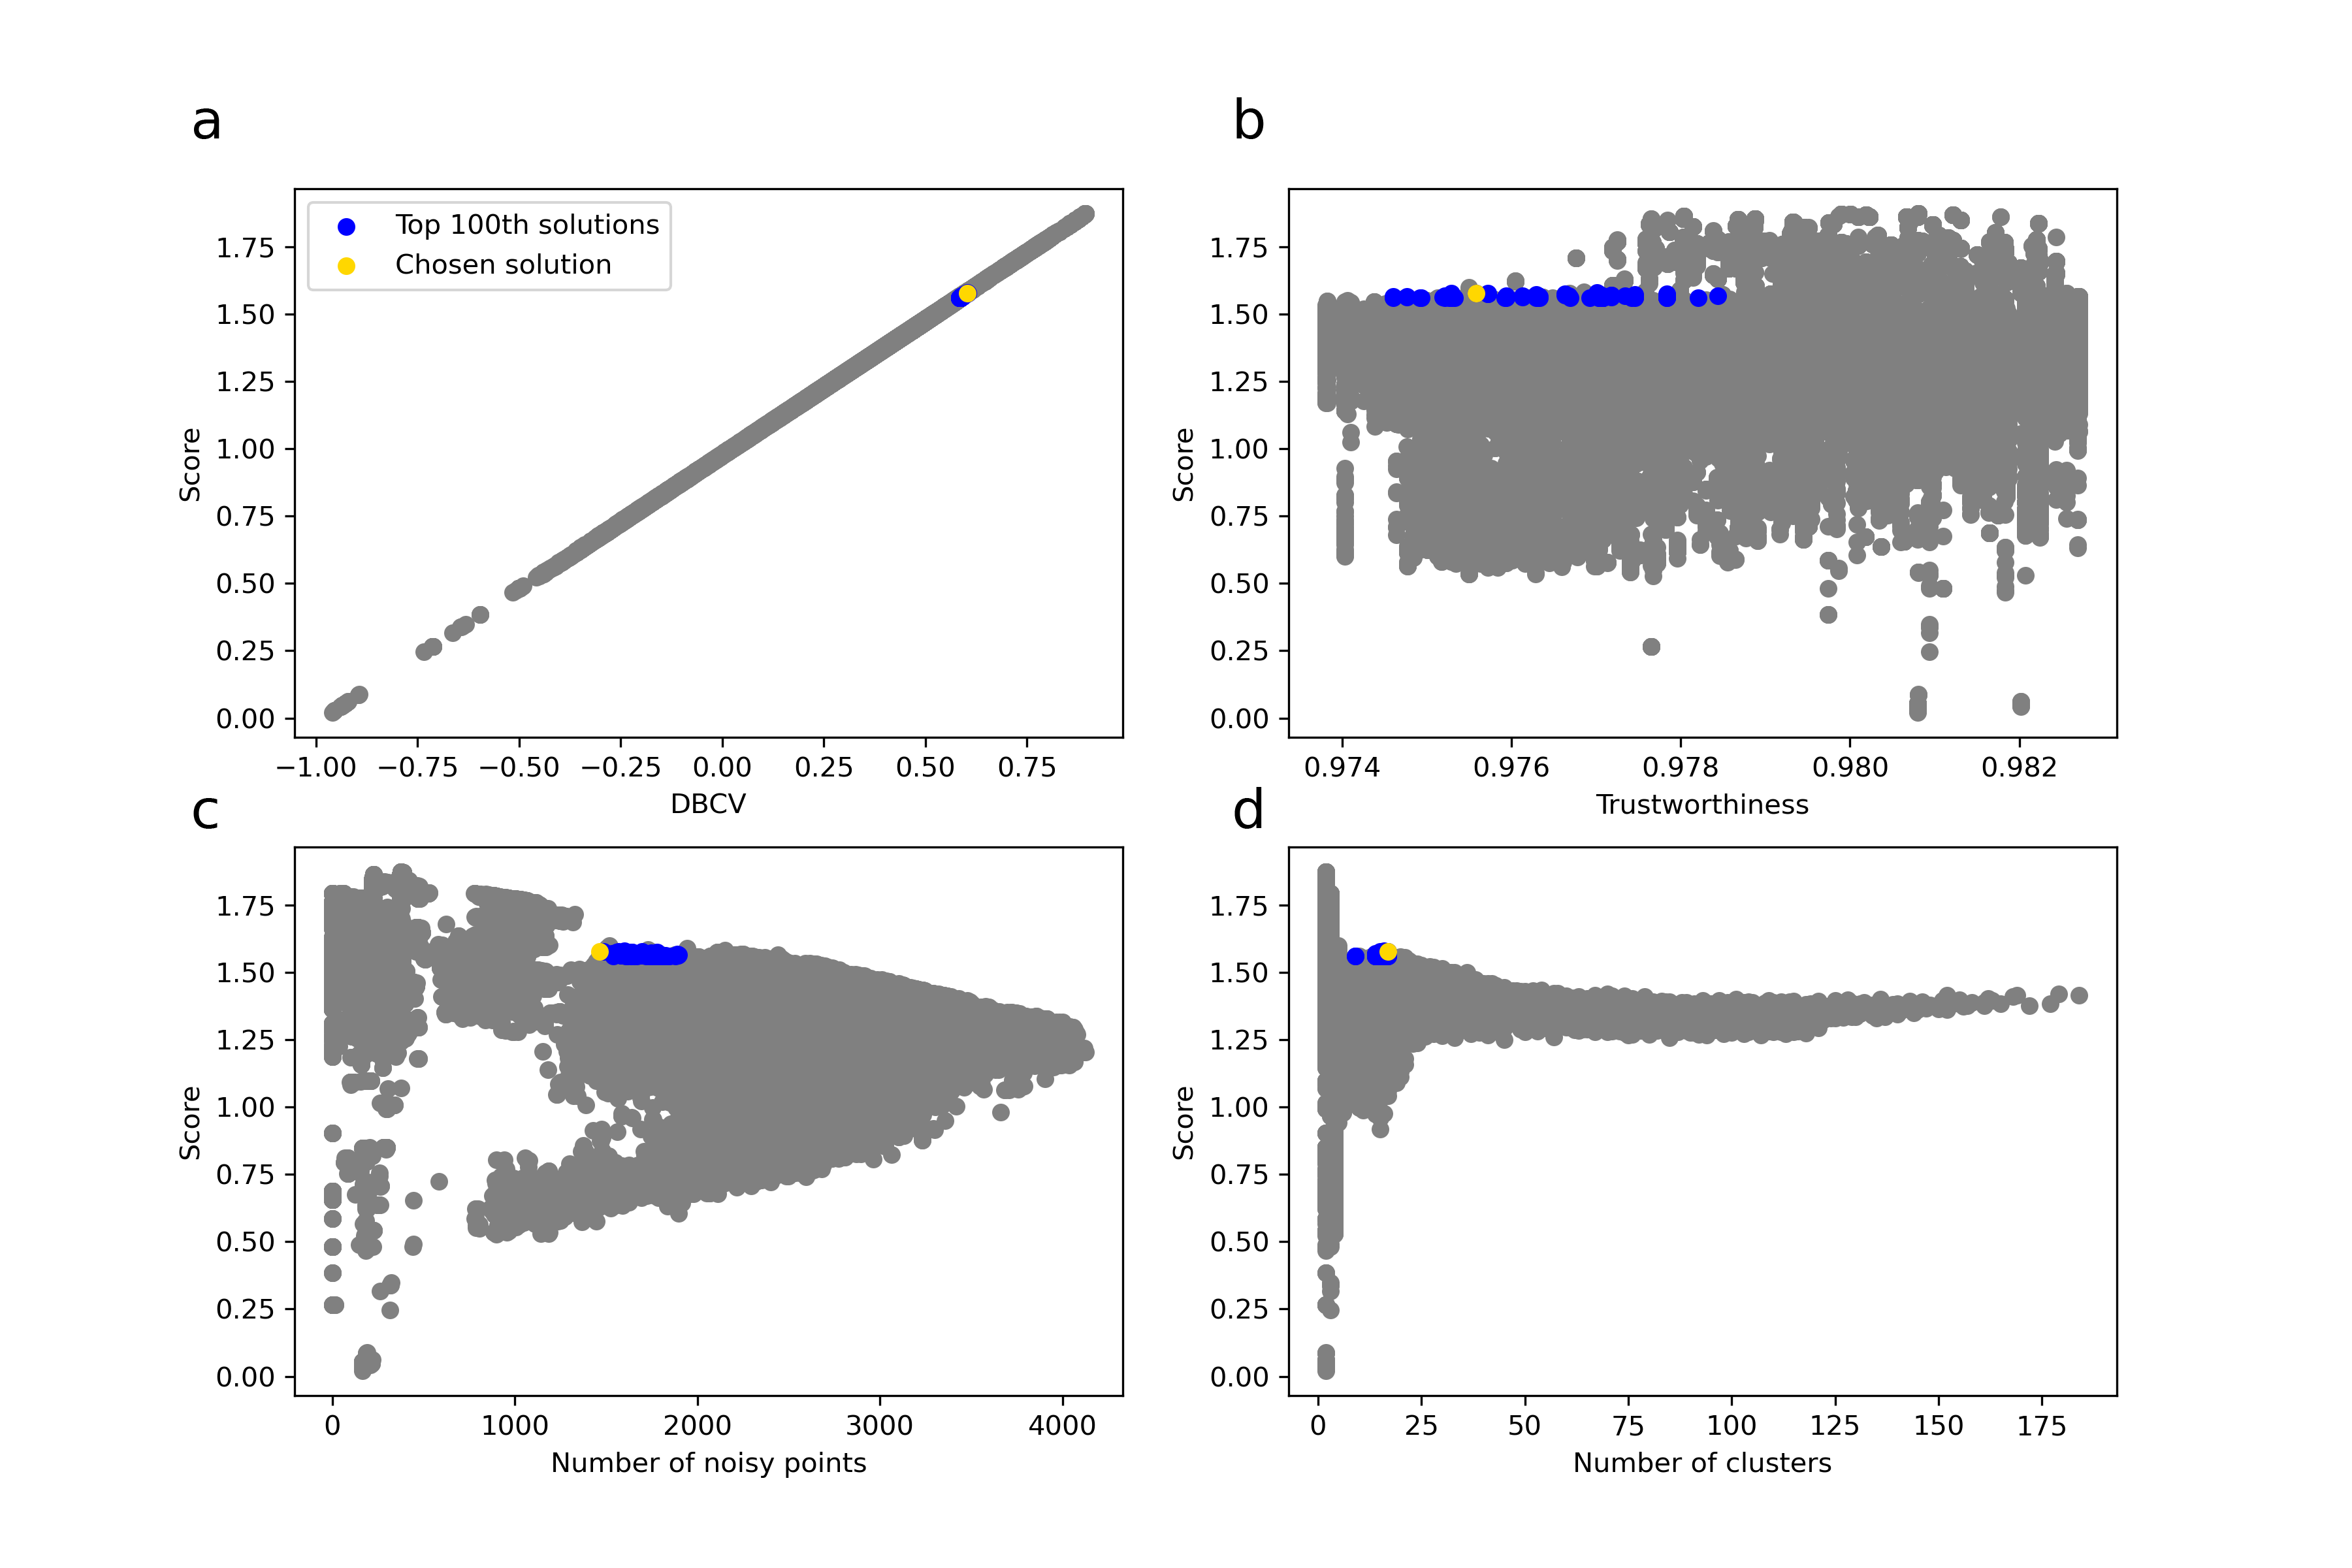
\includegraphics{03-Chapitre2/figures/supplementary/03-solutions-distributions.png}
\caption{Plot of the evolution of the score (i.e.~sum of the \emph{DBCV}
value and the Trustworthiness) according to the different parameters
measured (a. \emph{DBCV}; b. \emph{Trustworthiness}; c.~Number of noisy
points; d.~Number of clusters (the dotted line represents the number of
clusters uncovered by \textcite{Cresswell_2017})). Each of the 241,100
dots represent the evaluation of a unique combination of hyperparameter
values for \emph{UMAP} (\emph{n\_neighbors}) and \emph{HDBSCAN}
(\emph{min\_cluster\_size}). Blue dots represent the best solutions
with the higher \emph{DBCV} and \emph{Trustworthiness} having at least 9
groups, while the yellow dot represents the best solution found
according to our criteria. All other grey dots represent the other
evaluated solutions}\label{fig:chap2figS1}
}
\end{figure}

\begin{figure}
\hypertarget{fig:chap2figS2}{%
\centering
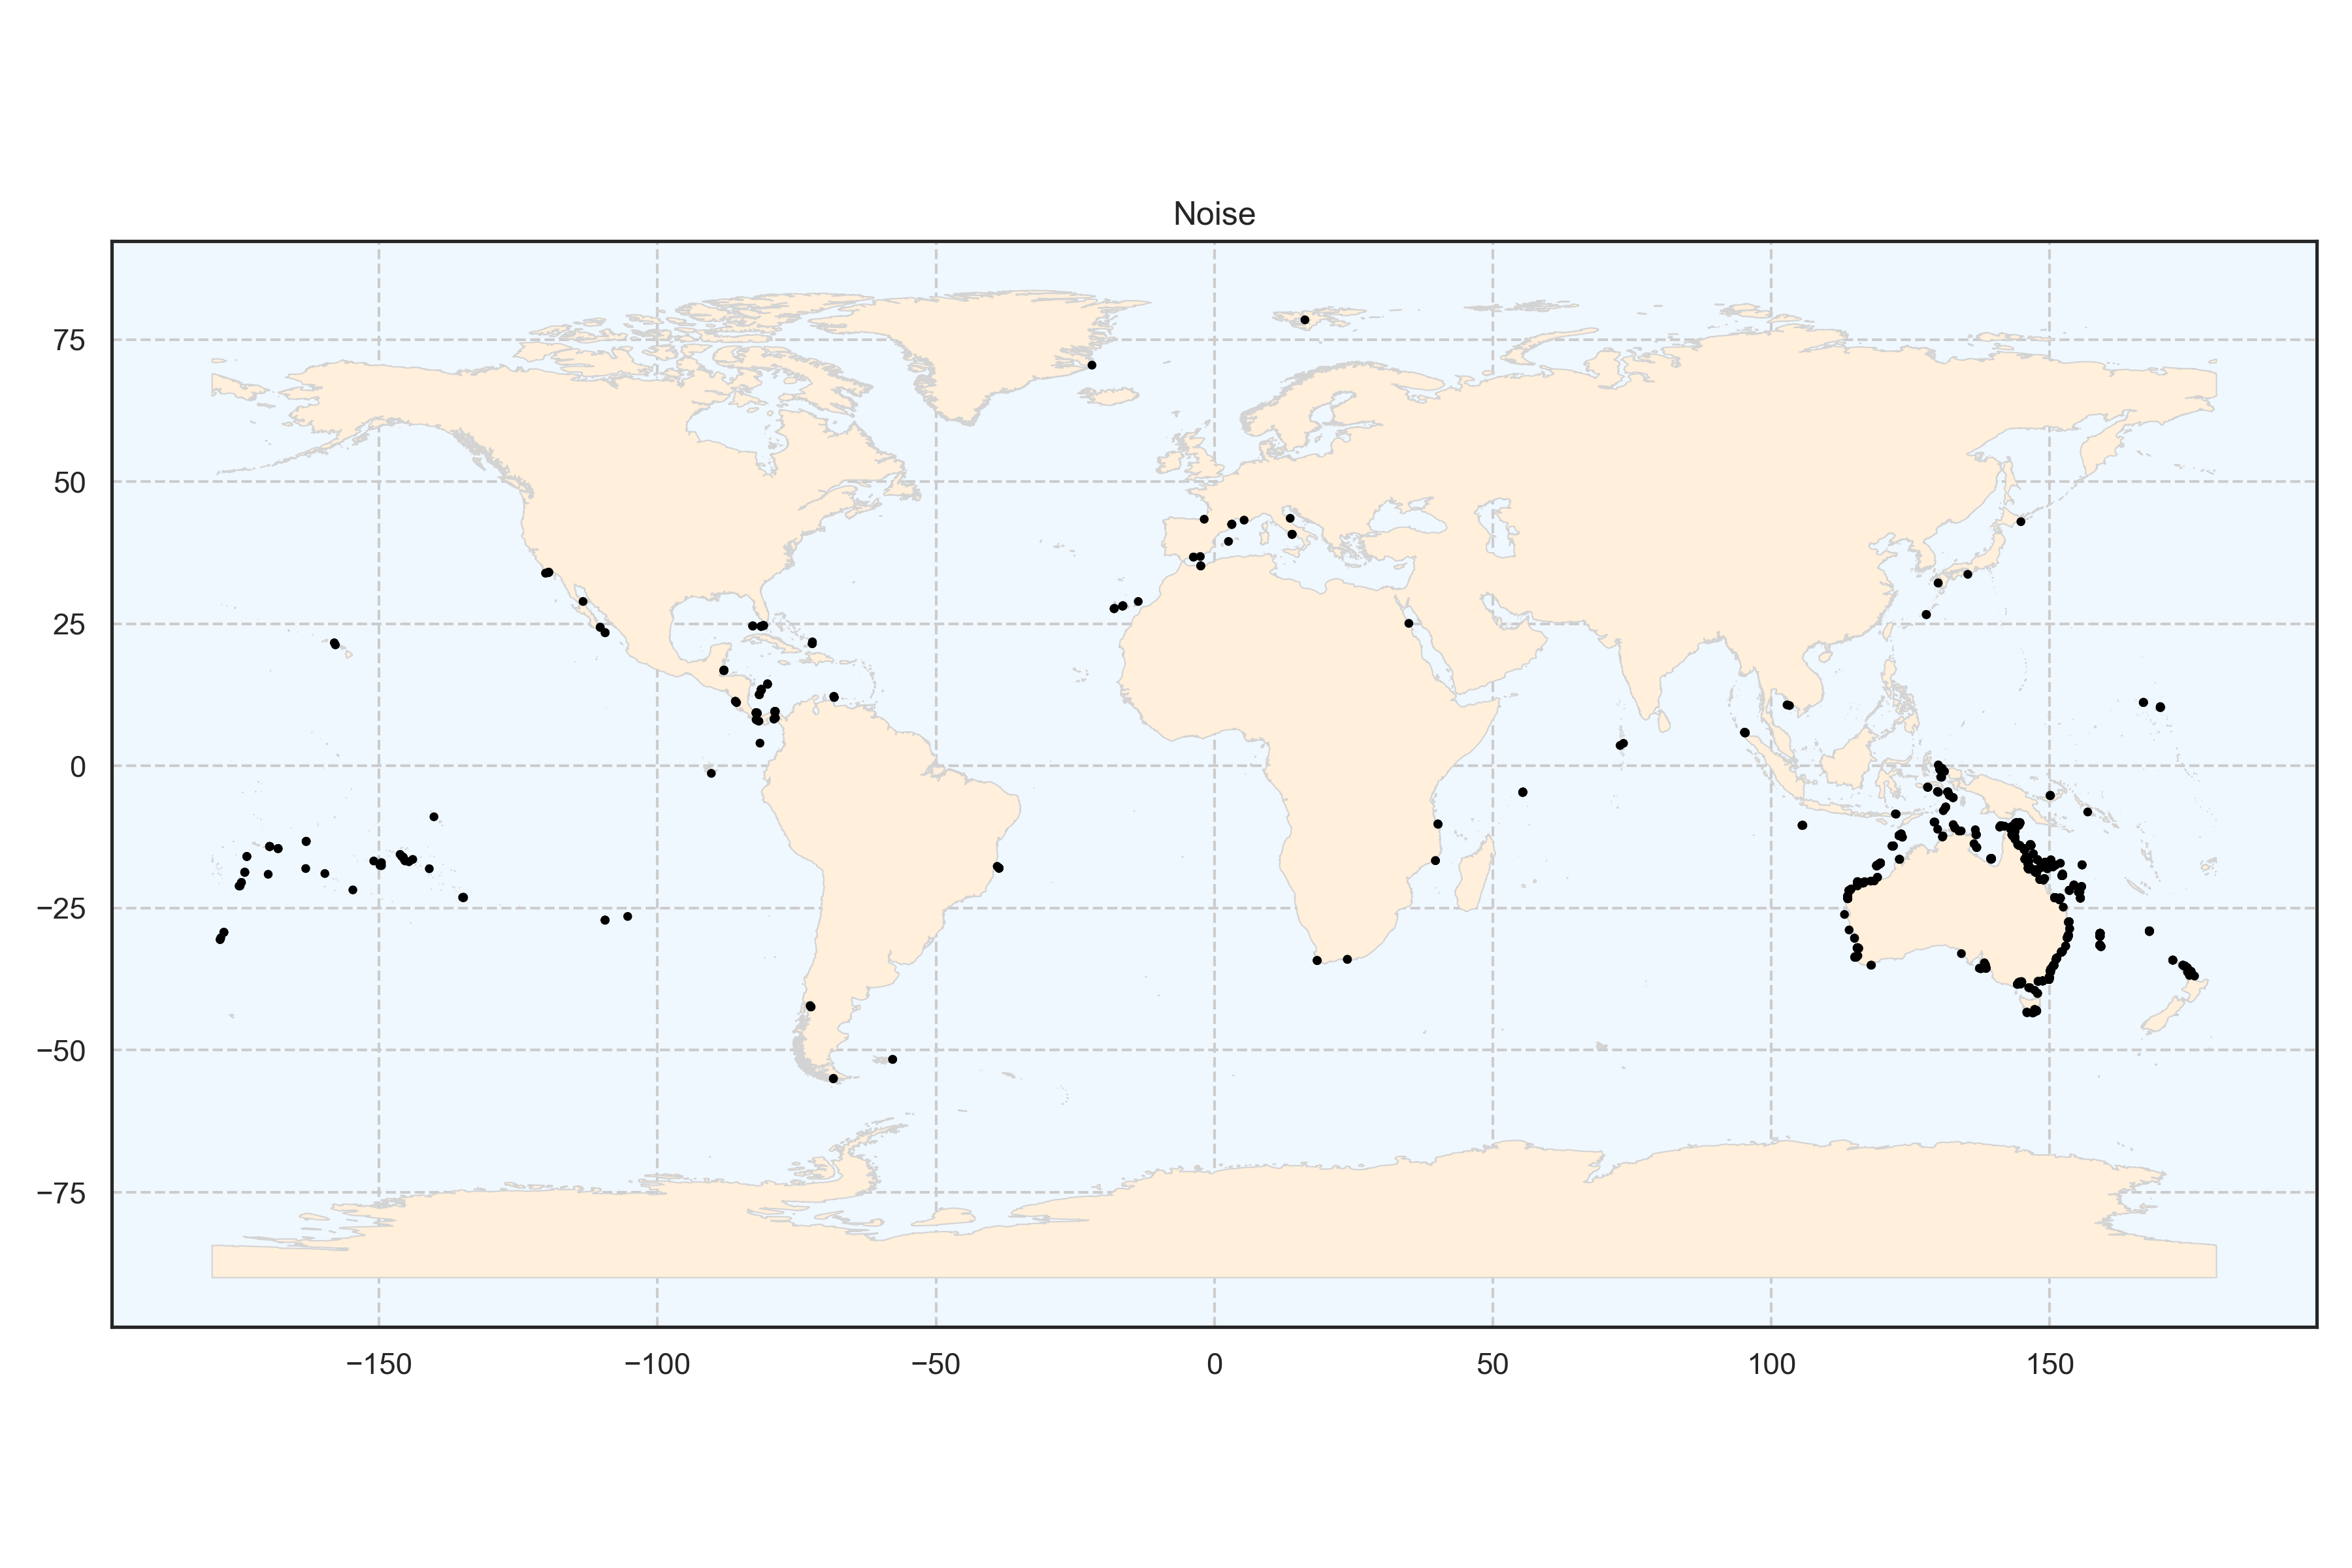
\includegraphics{03-Chapitre2/figures/supplementary/06-spatial-cluster_distribution_cluster_-1.png}
\caption{Spatial distribution of the cluster \emph{noise} at the global
scale. Each point represents a transect.}\label{fig:chap2figS2}
}
\end{figure}

\begin{figure}
\hypertarget{fig:chap2figS3}{%
\centering
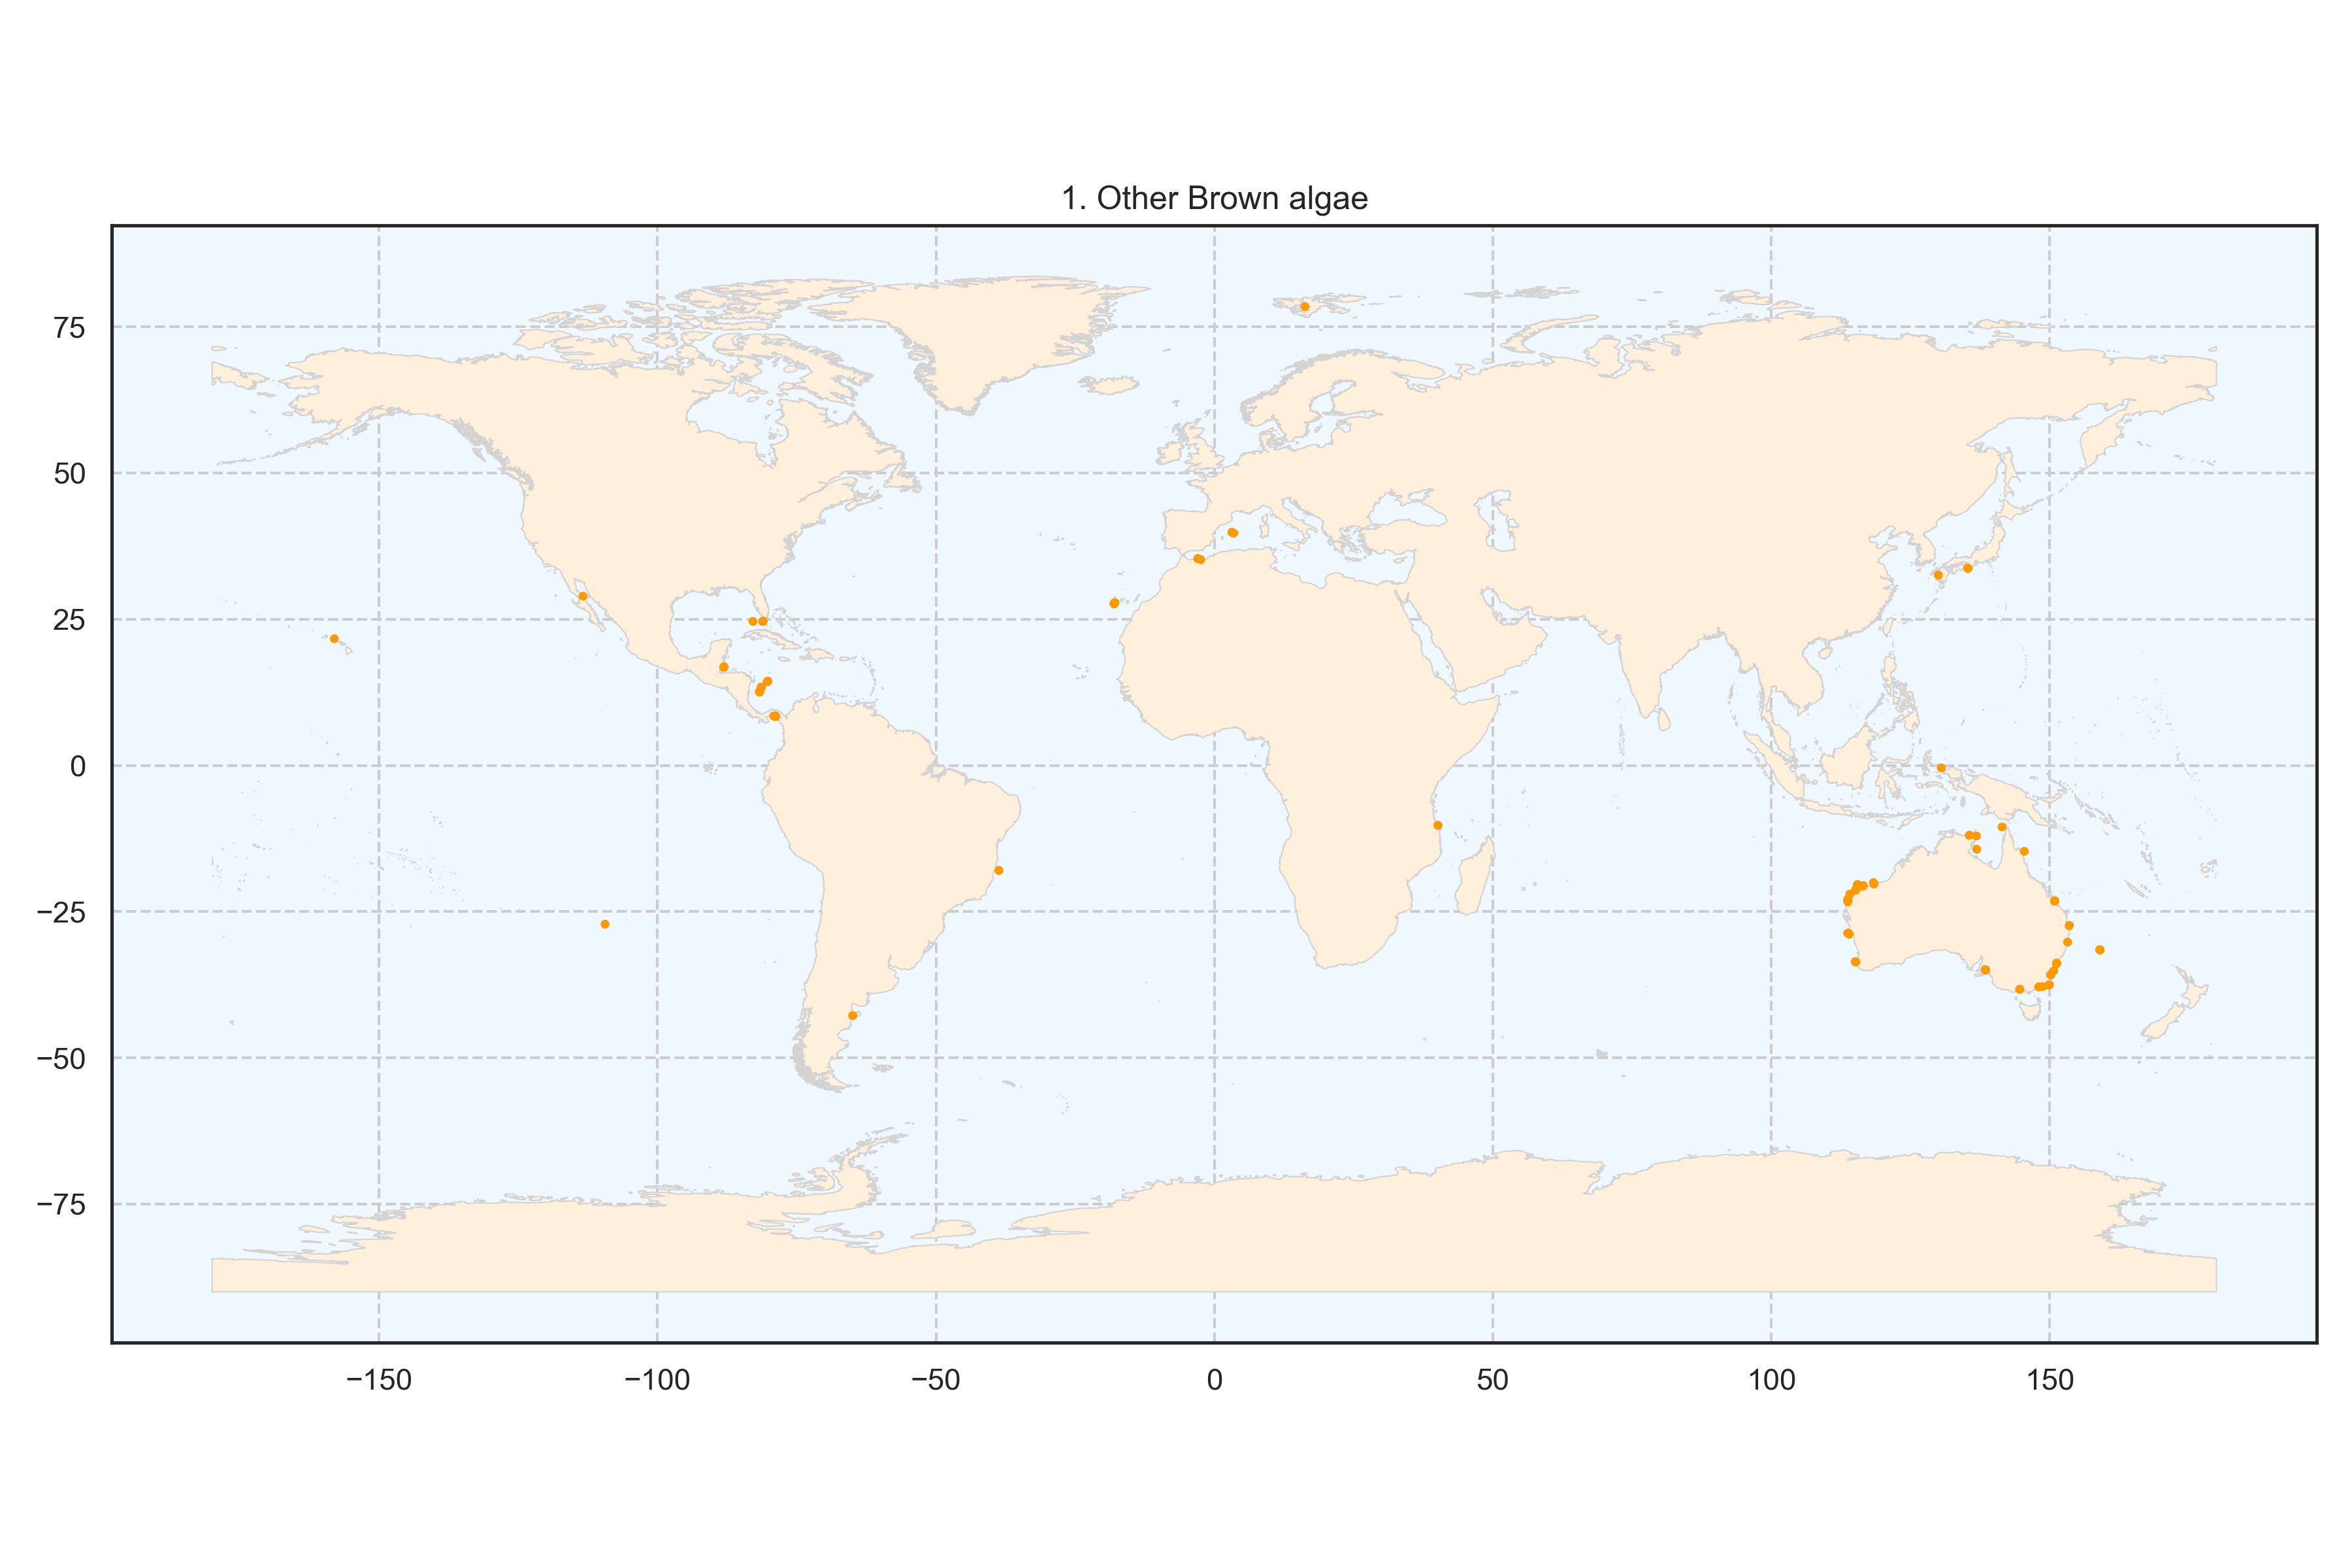
\includegraphics{03-Chapitre2/figures/supplementary/06-spatial-cluster_distribution_cluster_0.png}
\caption{Spatial distribution of the cluster \emph{foliose brown algae}
at the global scale. Each point represents a
transect.}\label{fig:chap2figS3}
}
\end{figure}

\begin{figure}
\hypertarget{fig:chap2figS4}{%
\centering
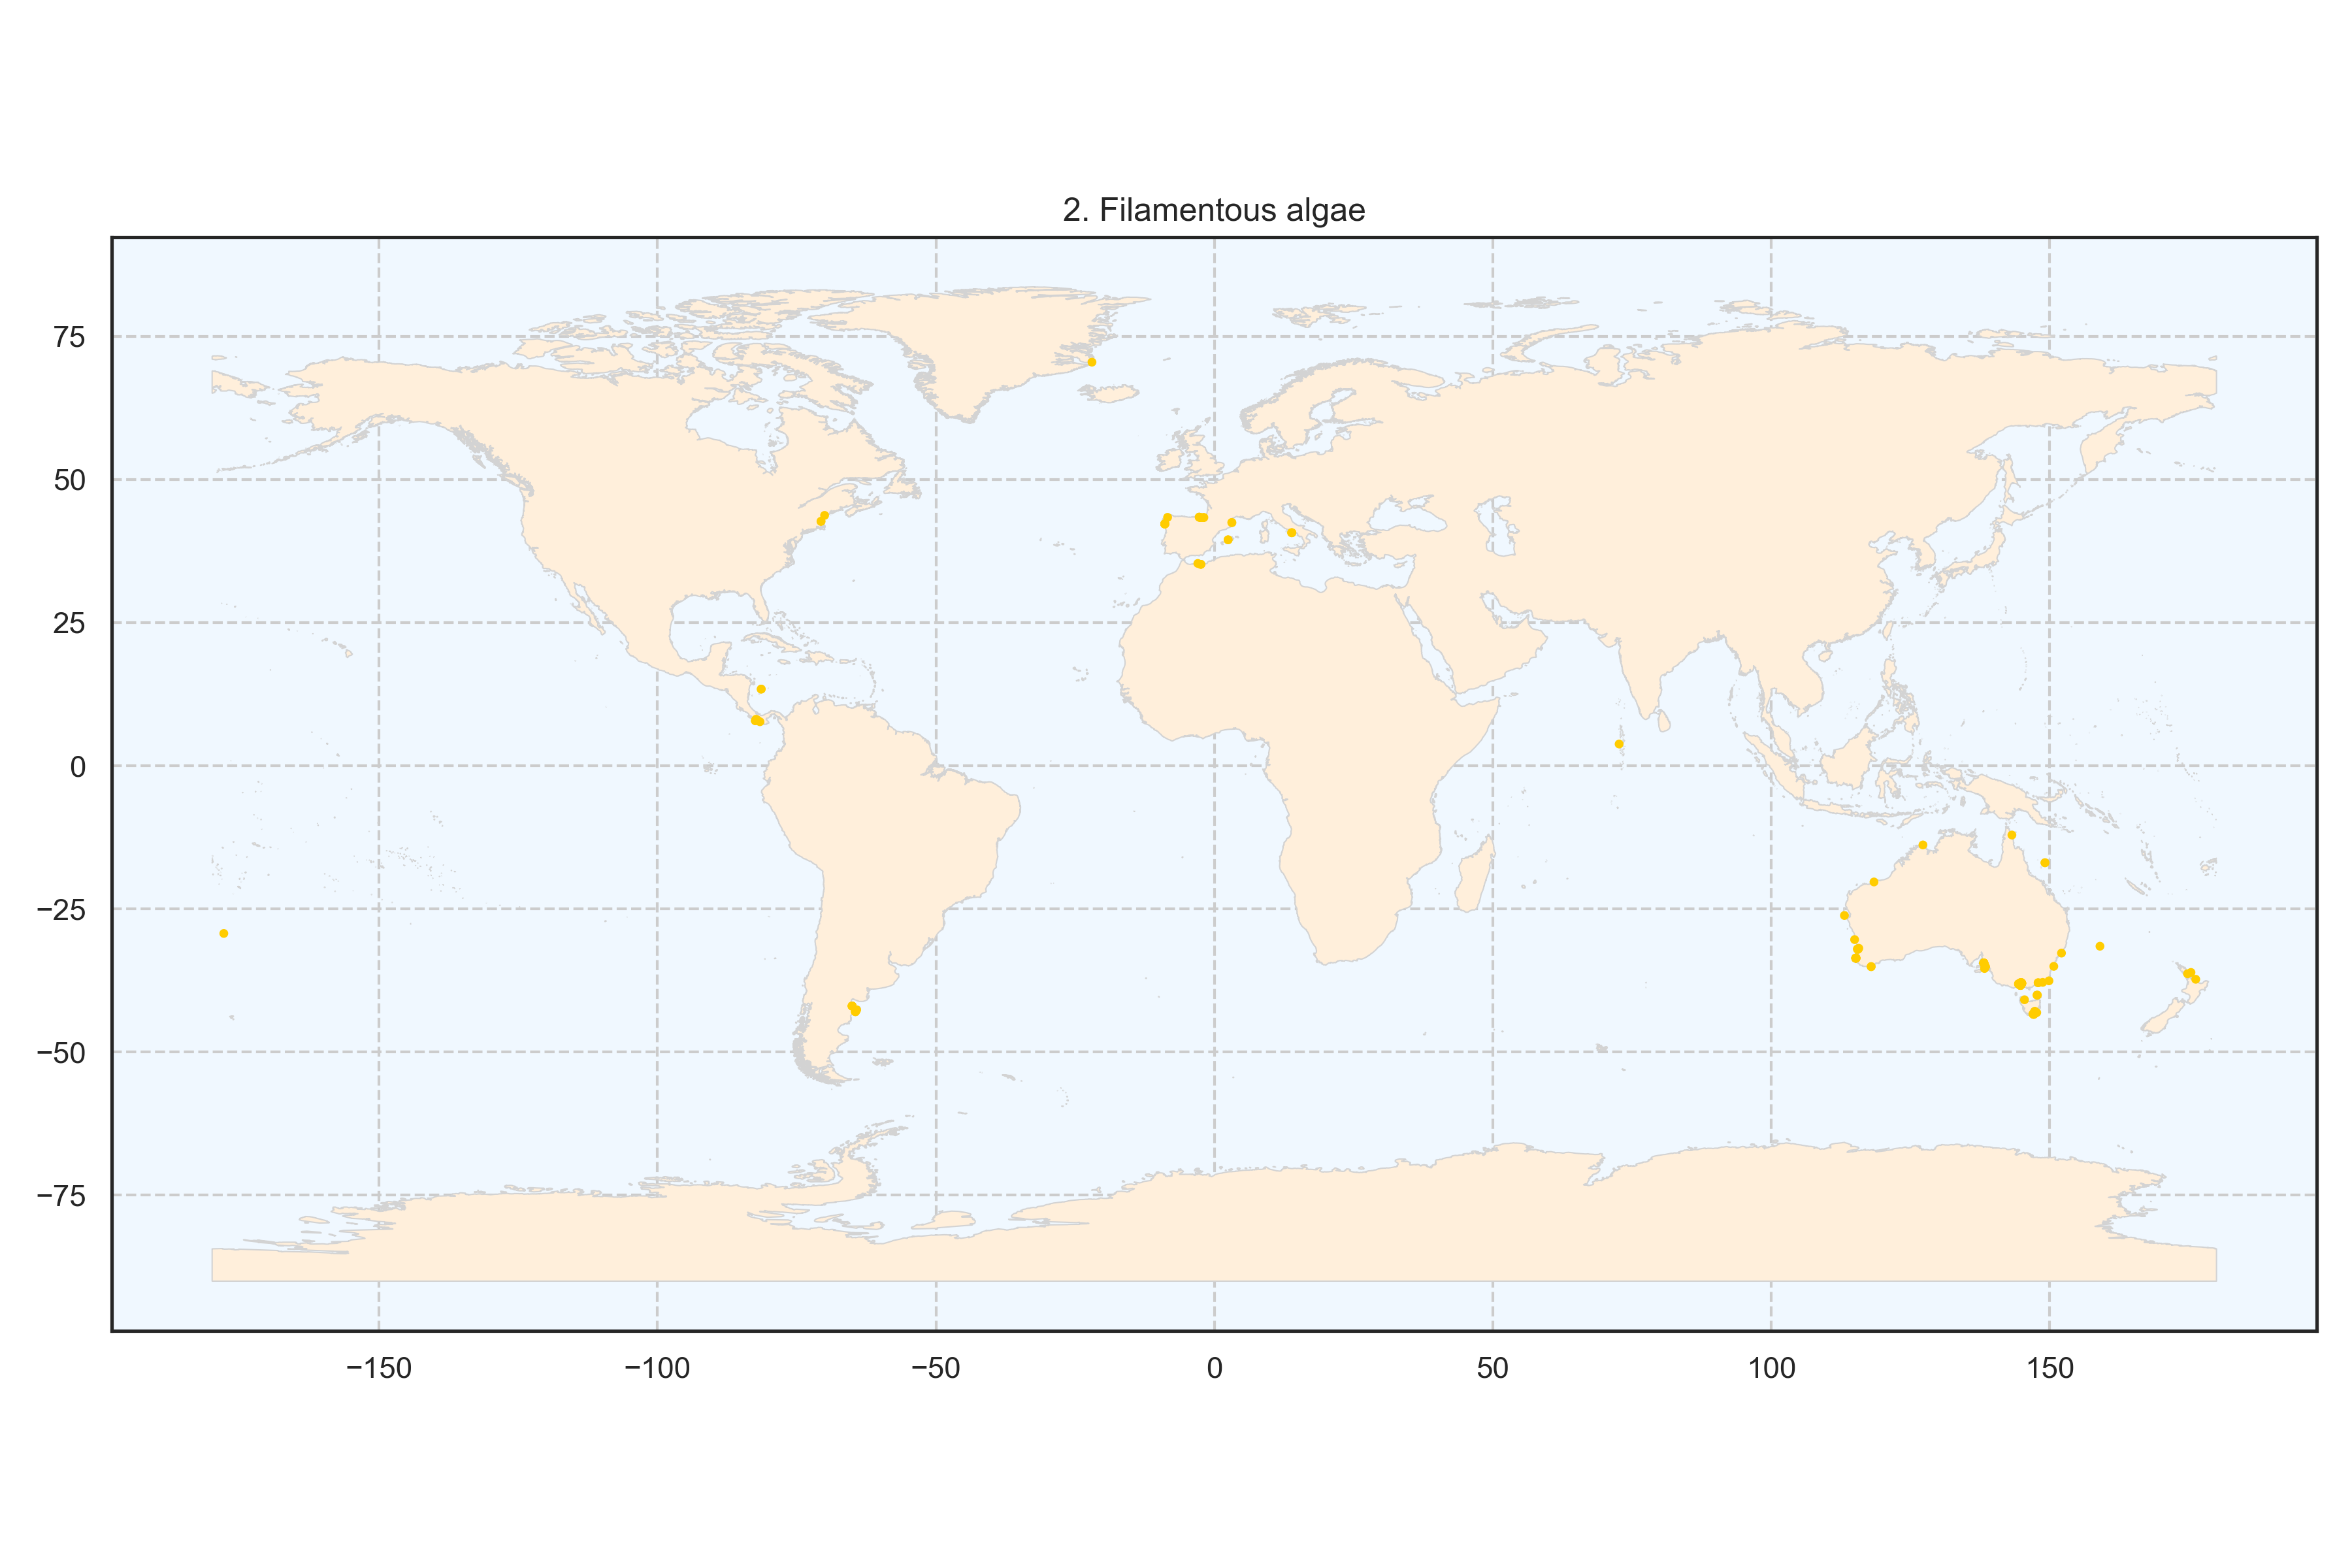
\includegraphics{03-Chapitre2/figures/supplementary/06-spatial-cluster_distribution_cluster_1.png}
\caption{Spatial distribution of the cluster \emph{filamentous algae} at
the global scale. Each point represents a
transect.}\label{fig:chap2figS4}
}
\end{figure}

\begin{figure}
\hypertarget{fig:chap2figS5}{%
\centering
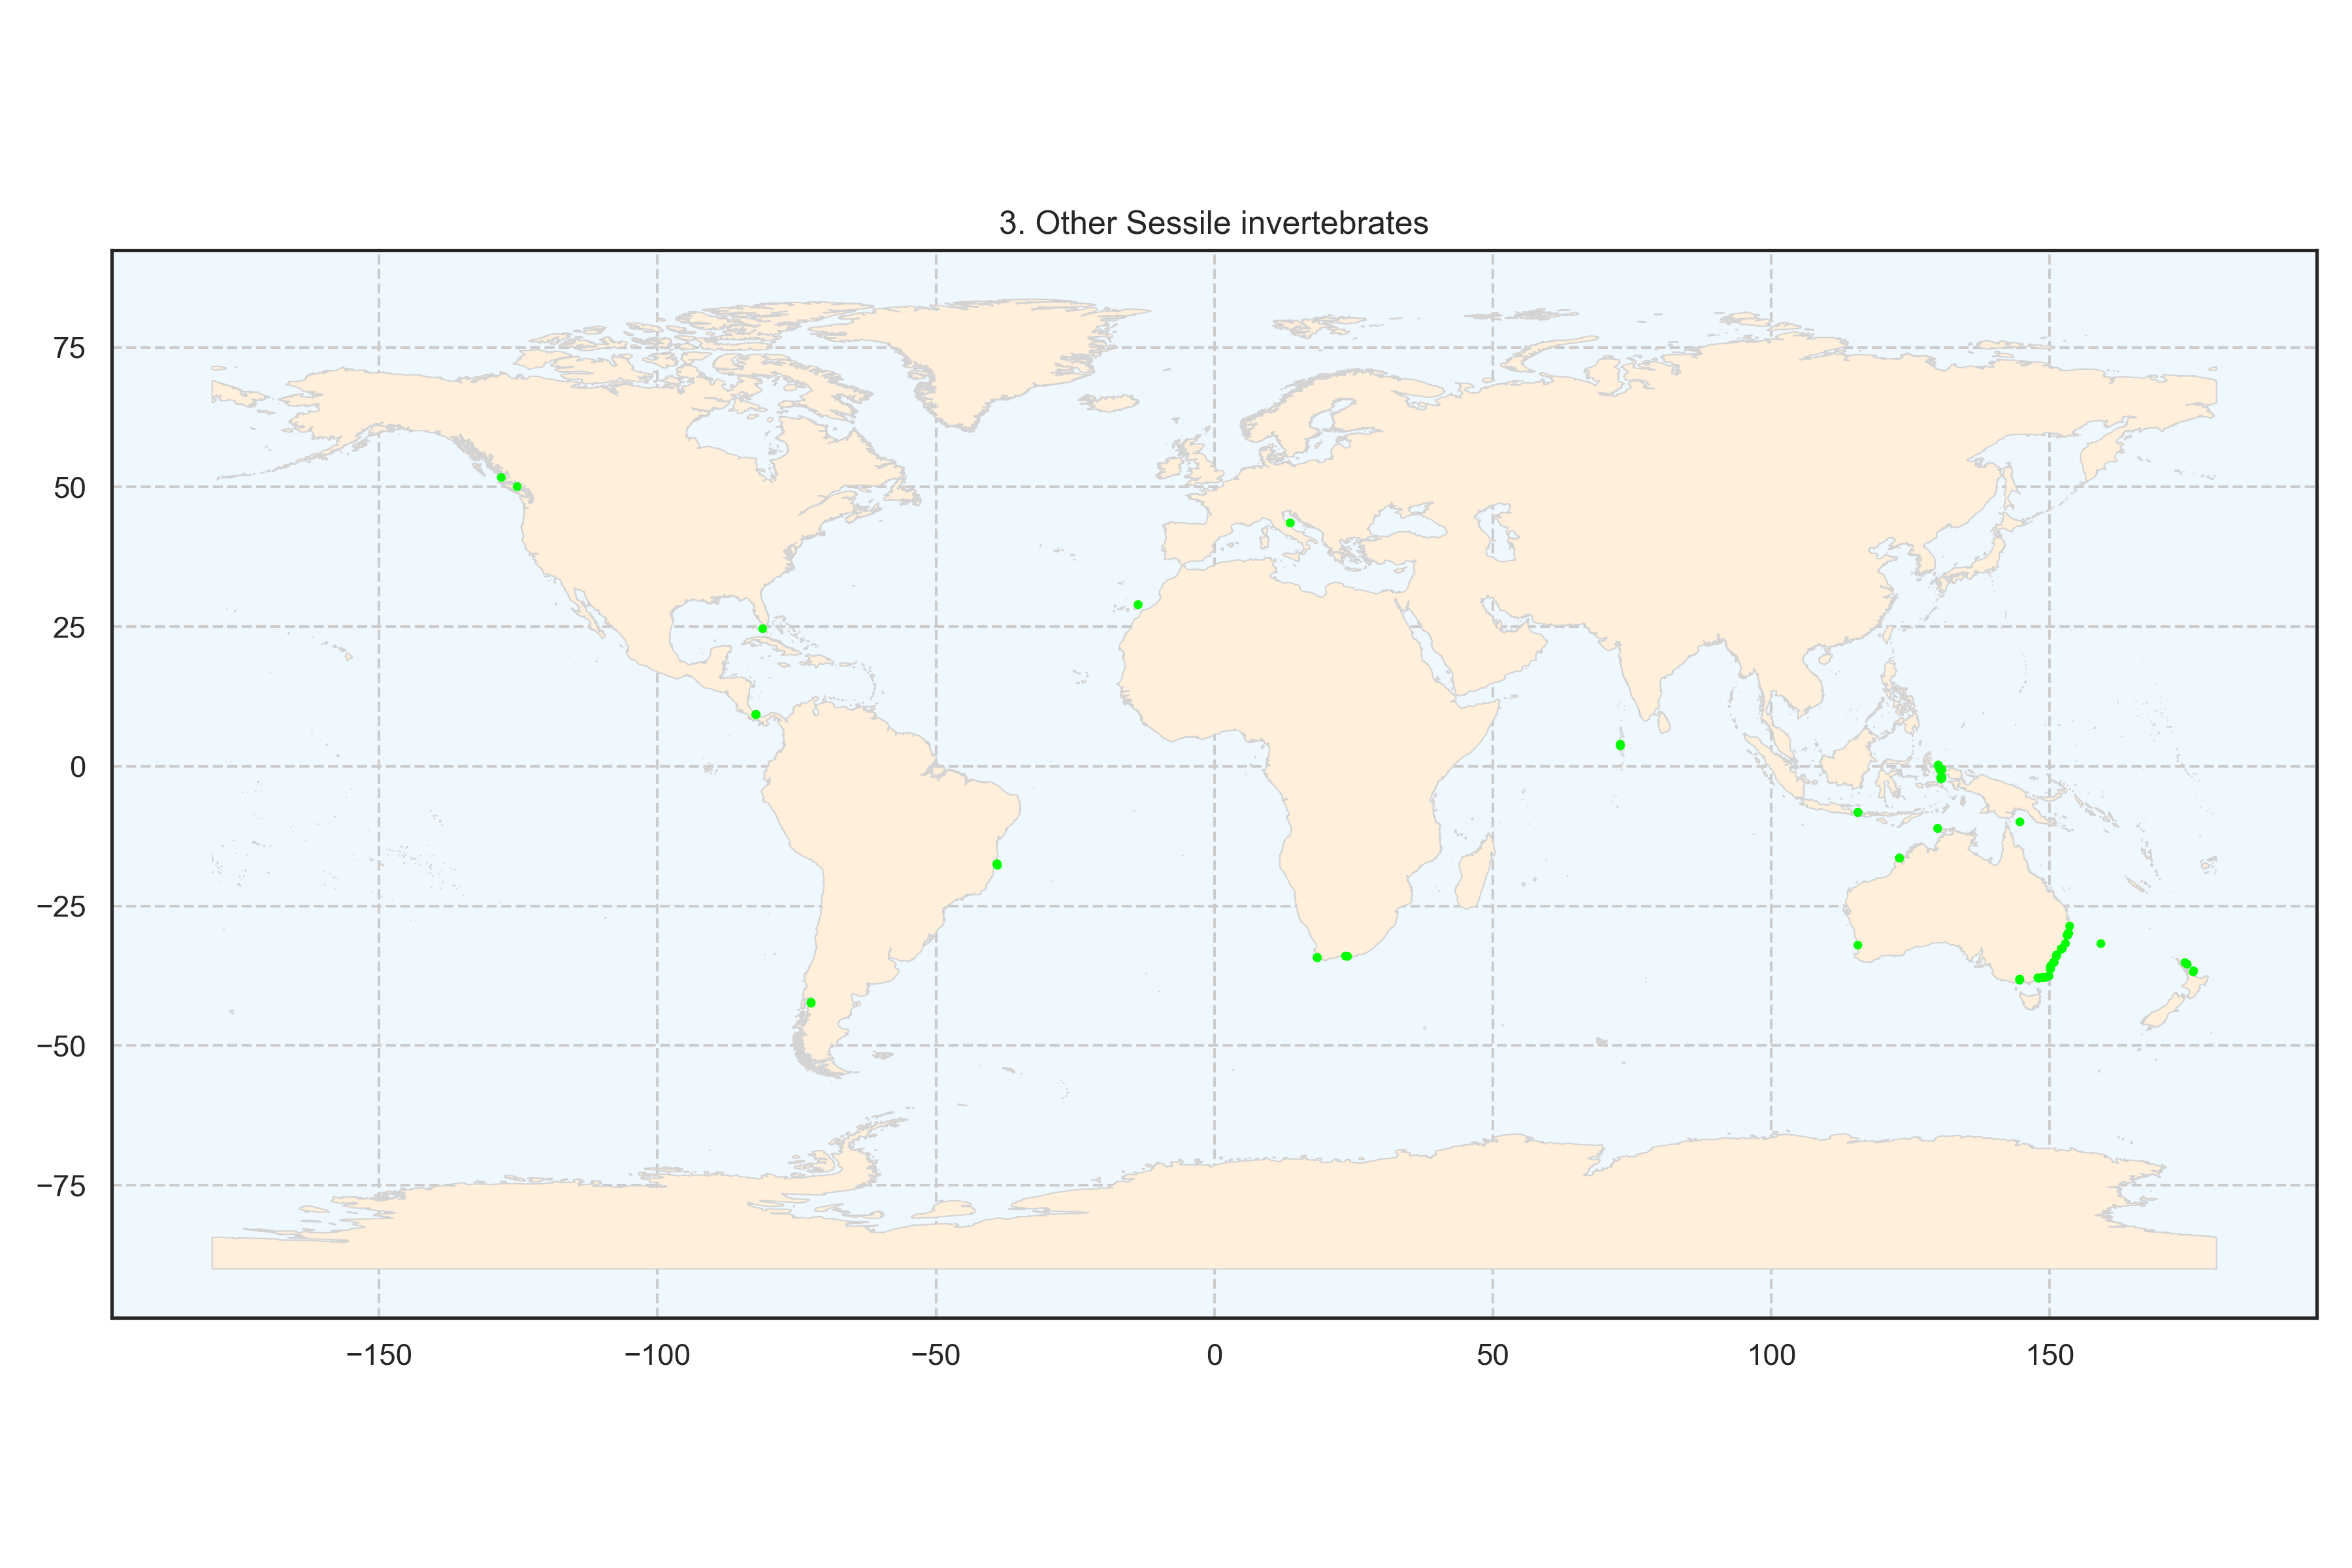
\includegraphics{03-Chapitre2/figures/supplementary/06-spatial-cluster_distribution_cluster_2.png}
\caption{Spatial distribution of the cluster \emph{other Sessile
invertebrates} at the global scale. Each point represents a
transect.}\label{fig:chap2figS5}
}
\end{figure}

\begin{figure}
\hypertarget{fig:chap2figS6}{%
\centering
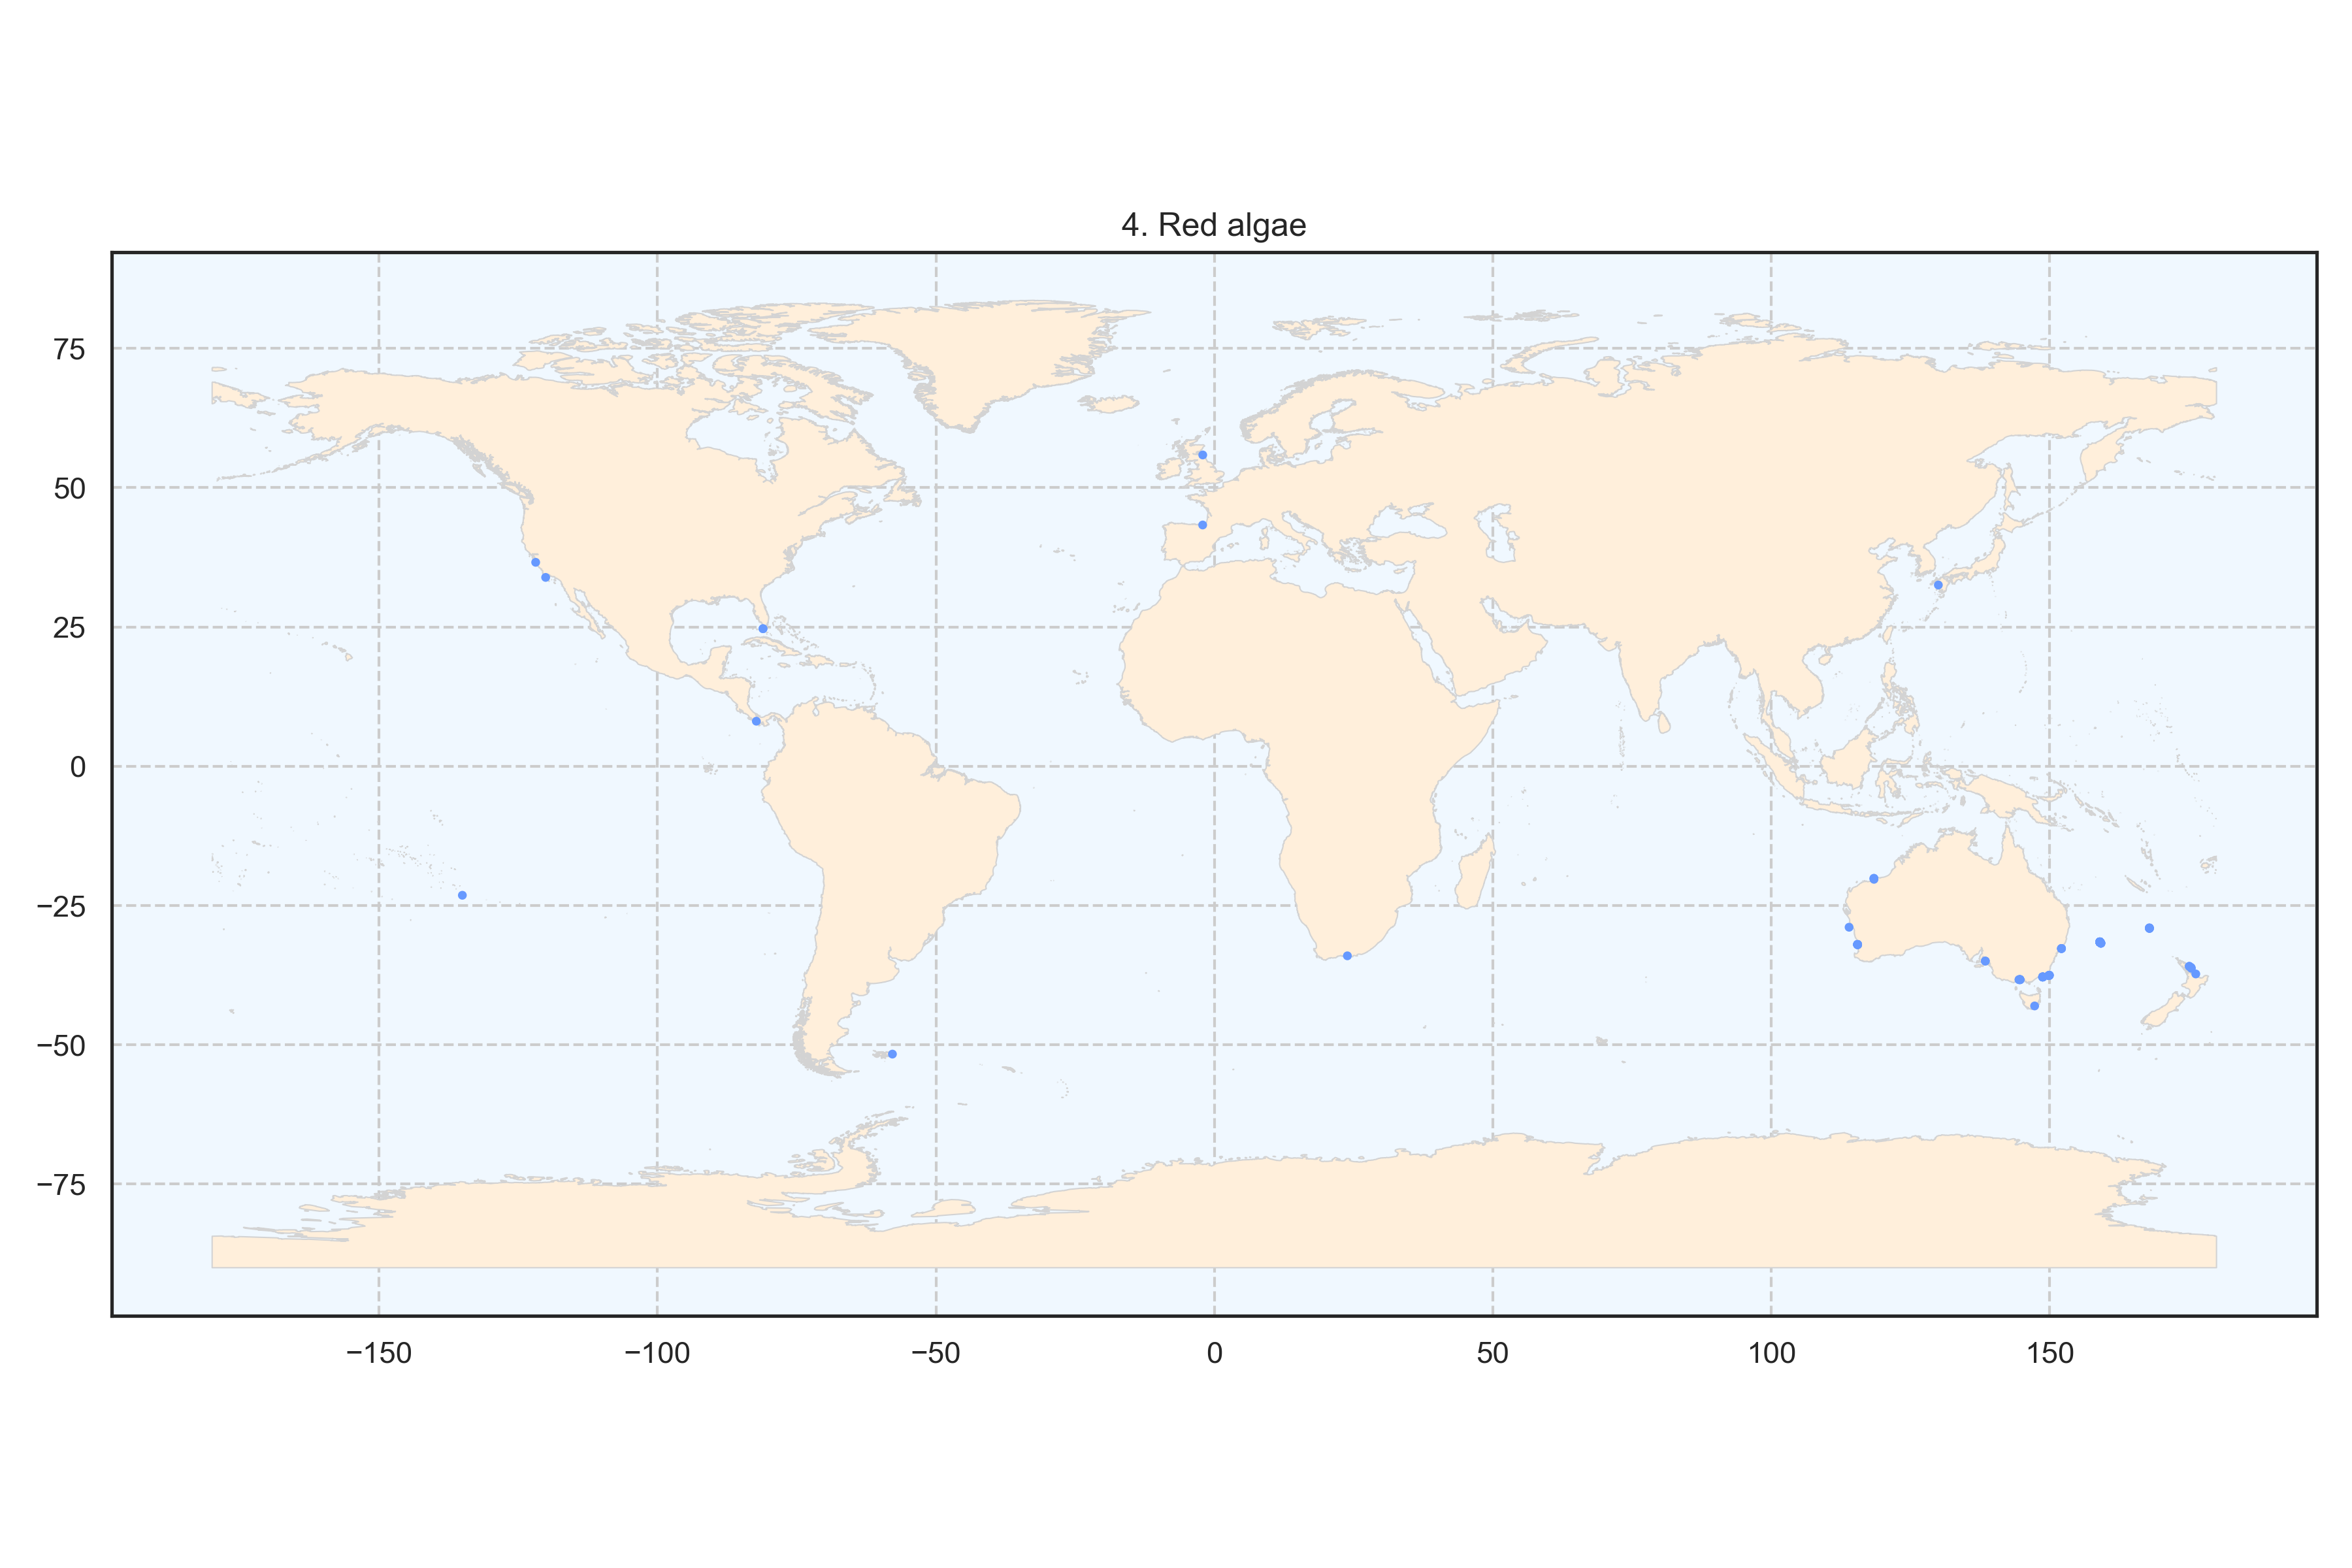
\includegraphics{03-Chapitre2/figures/supplementary/06-spatial-cluster_distribution_cluster_3.png}
\caption{Spatial distribution of the cluster \emph{red algae} at the
global scale. Each point represents a transect.}\label{fig:chap2figS6}
}
\end{figure}

\begin{figure}
\hypertarget{fig:chap2figS7}{%
\centering
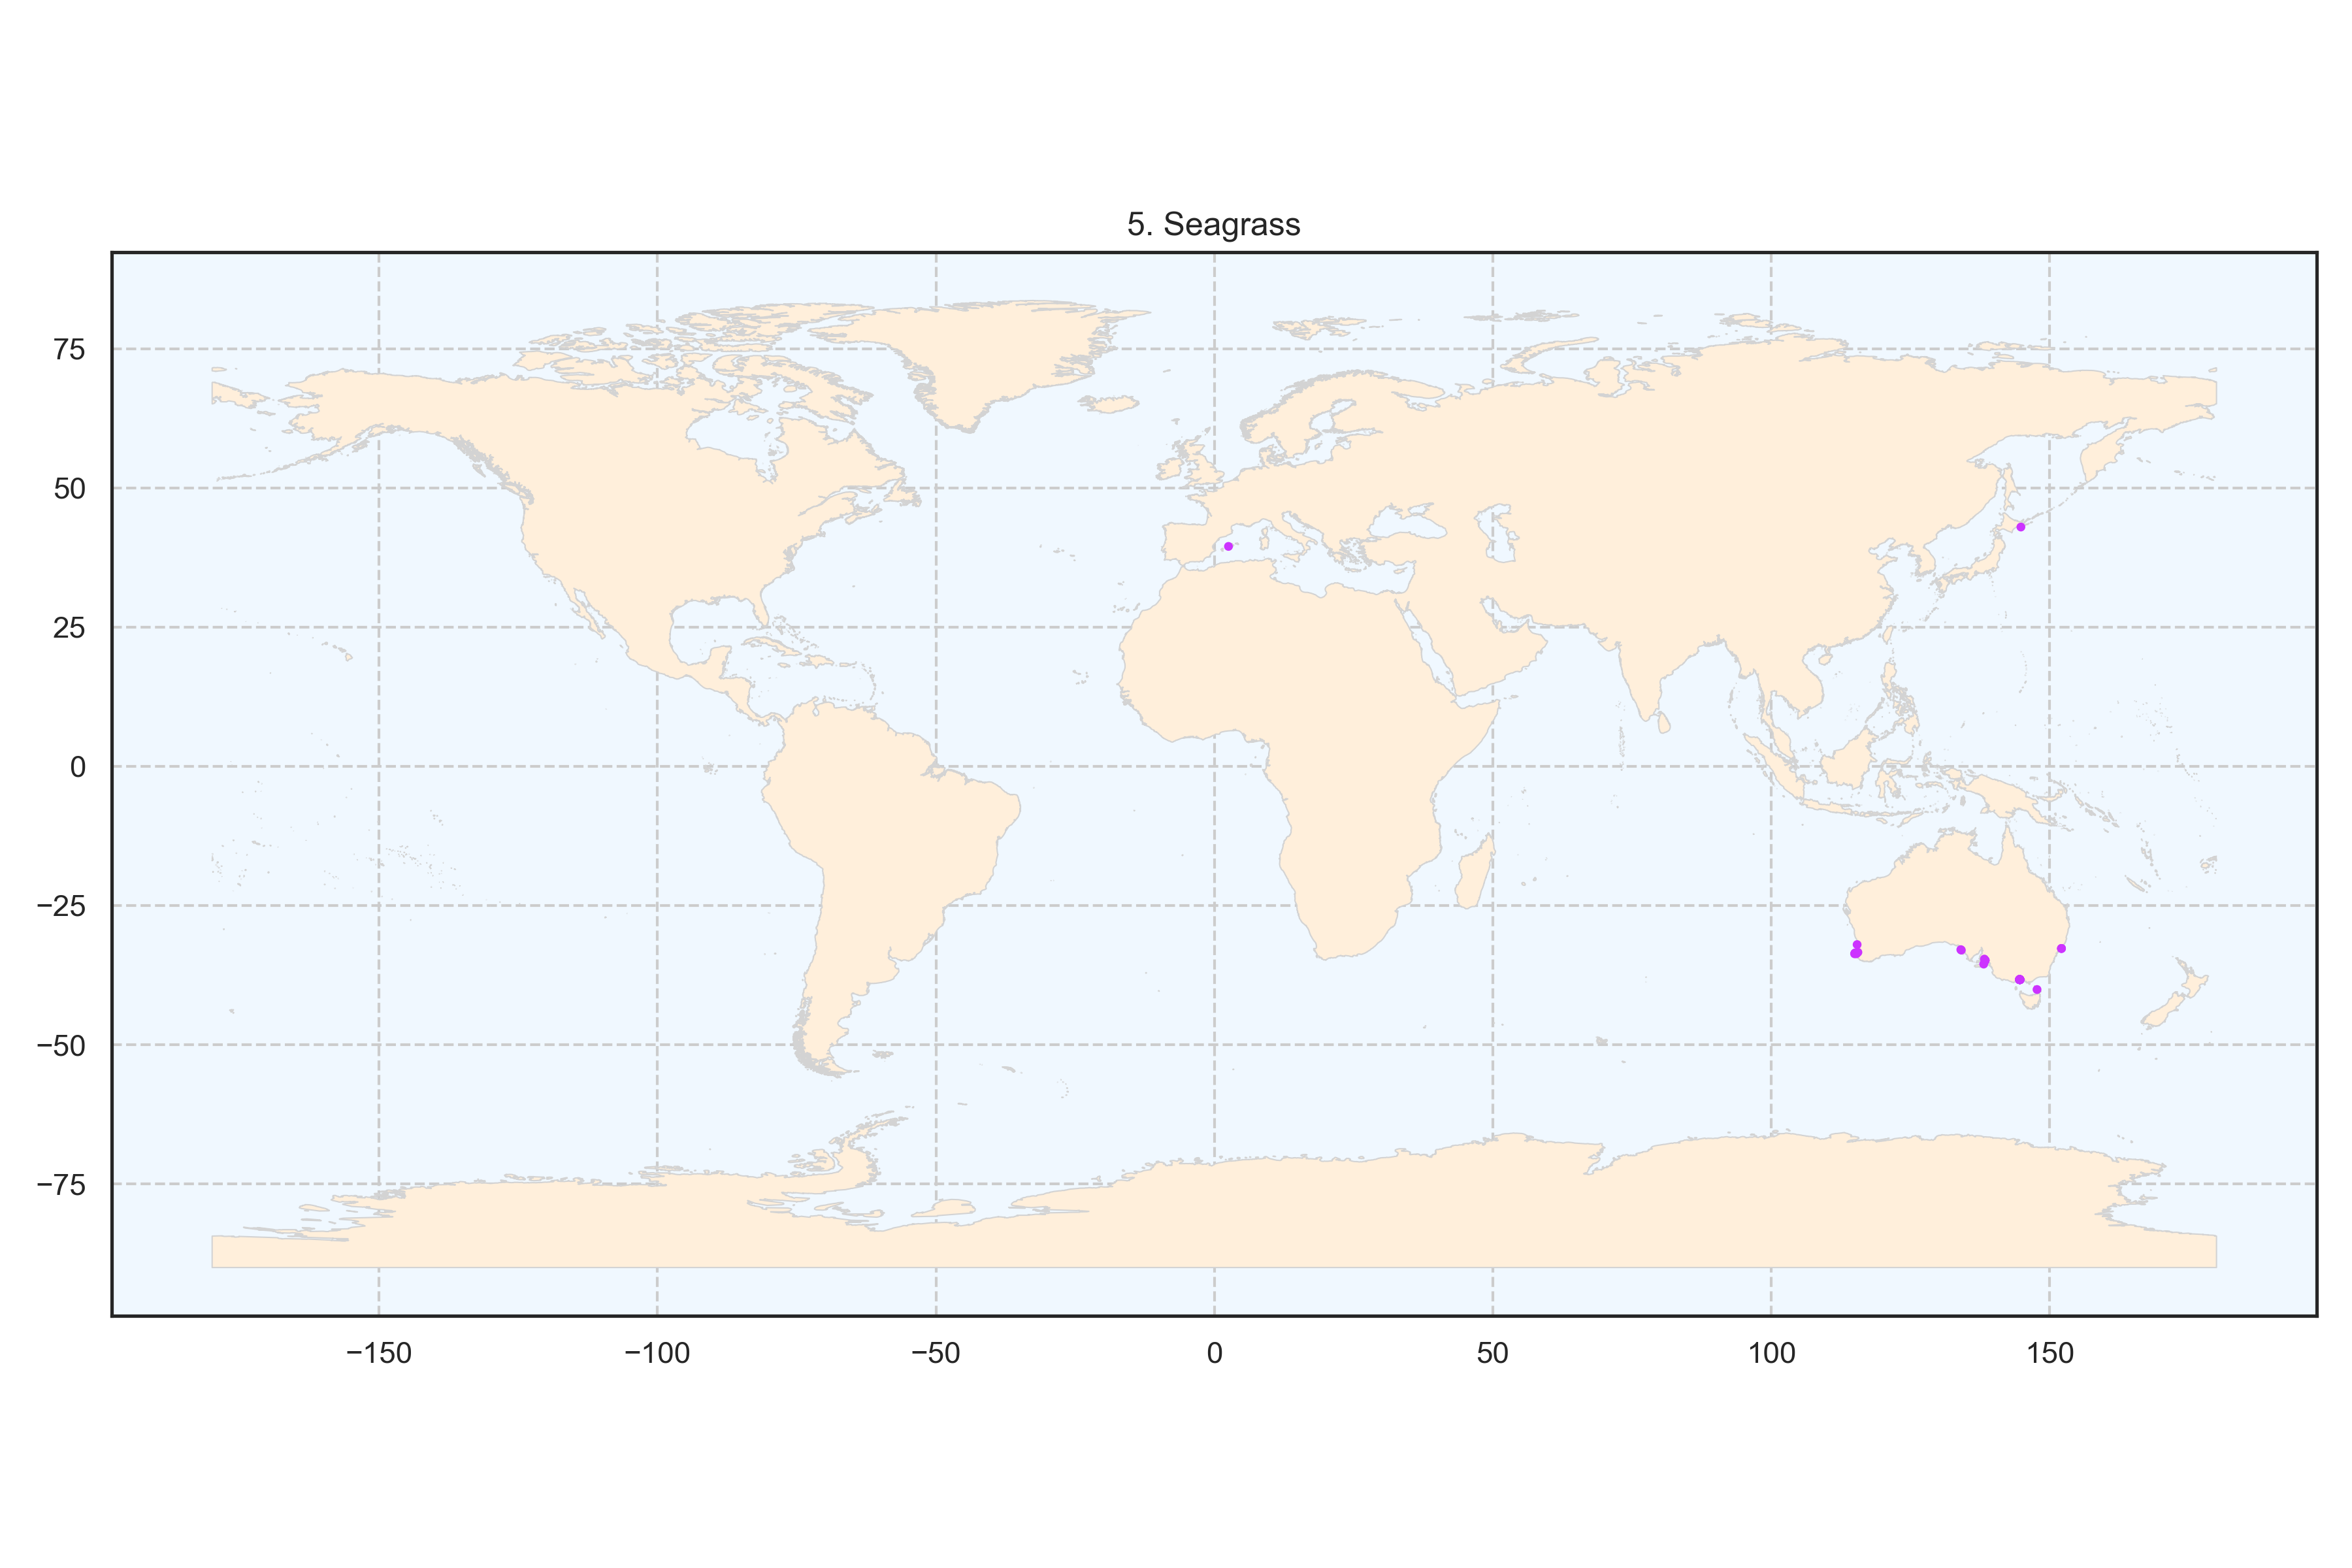
\includegraphics{03-Chapitre2/figures/supplementary/06-spatial-cluster_distribution_cluster_4.png}
\caption{Spatial distribution of the cluster \emph{seagrass} at the
global scale. Each point represents a transect.}\label{fig:chap2figS7}
}
\end{figure}

\begin{figure}
\hypertarget{fig:chap2figS8}{%
\centering
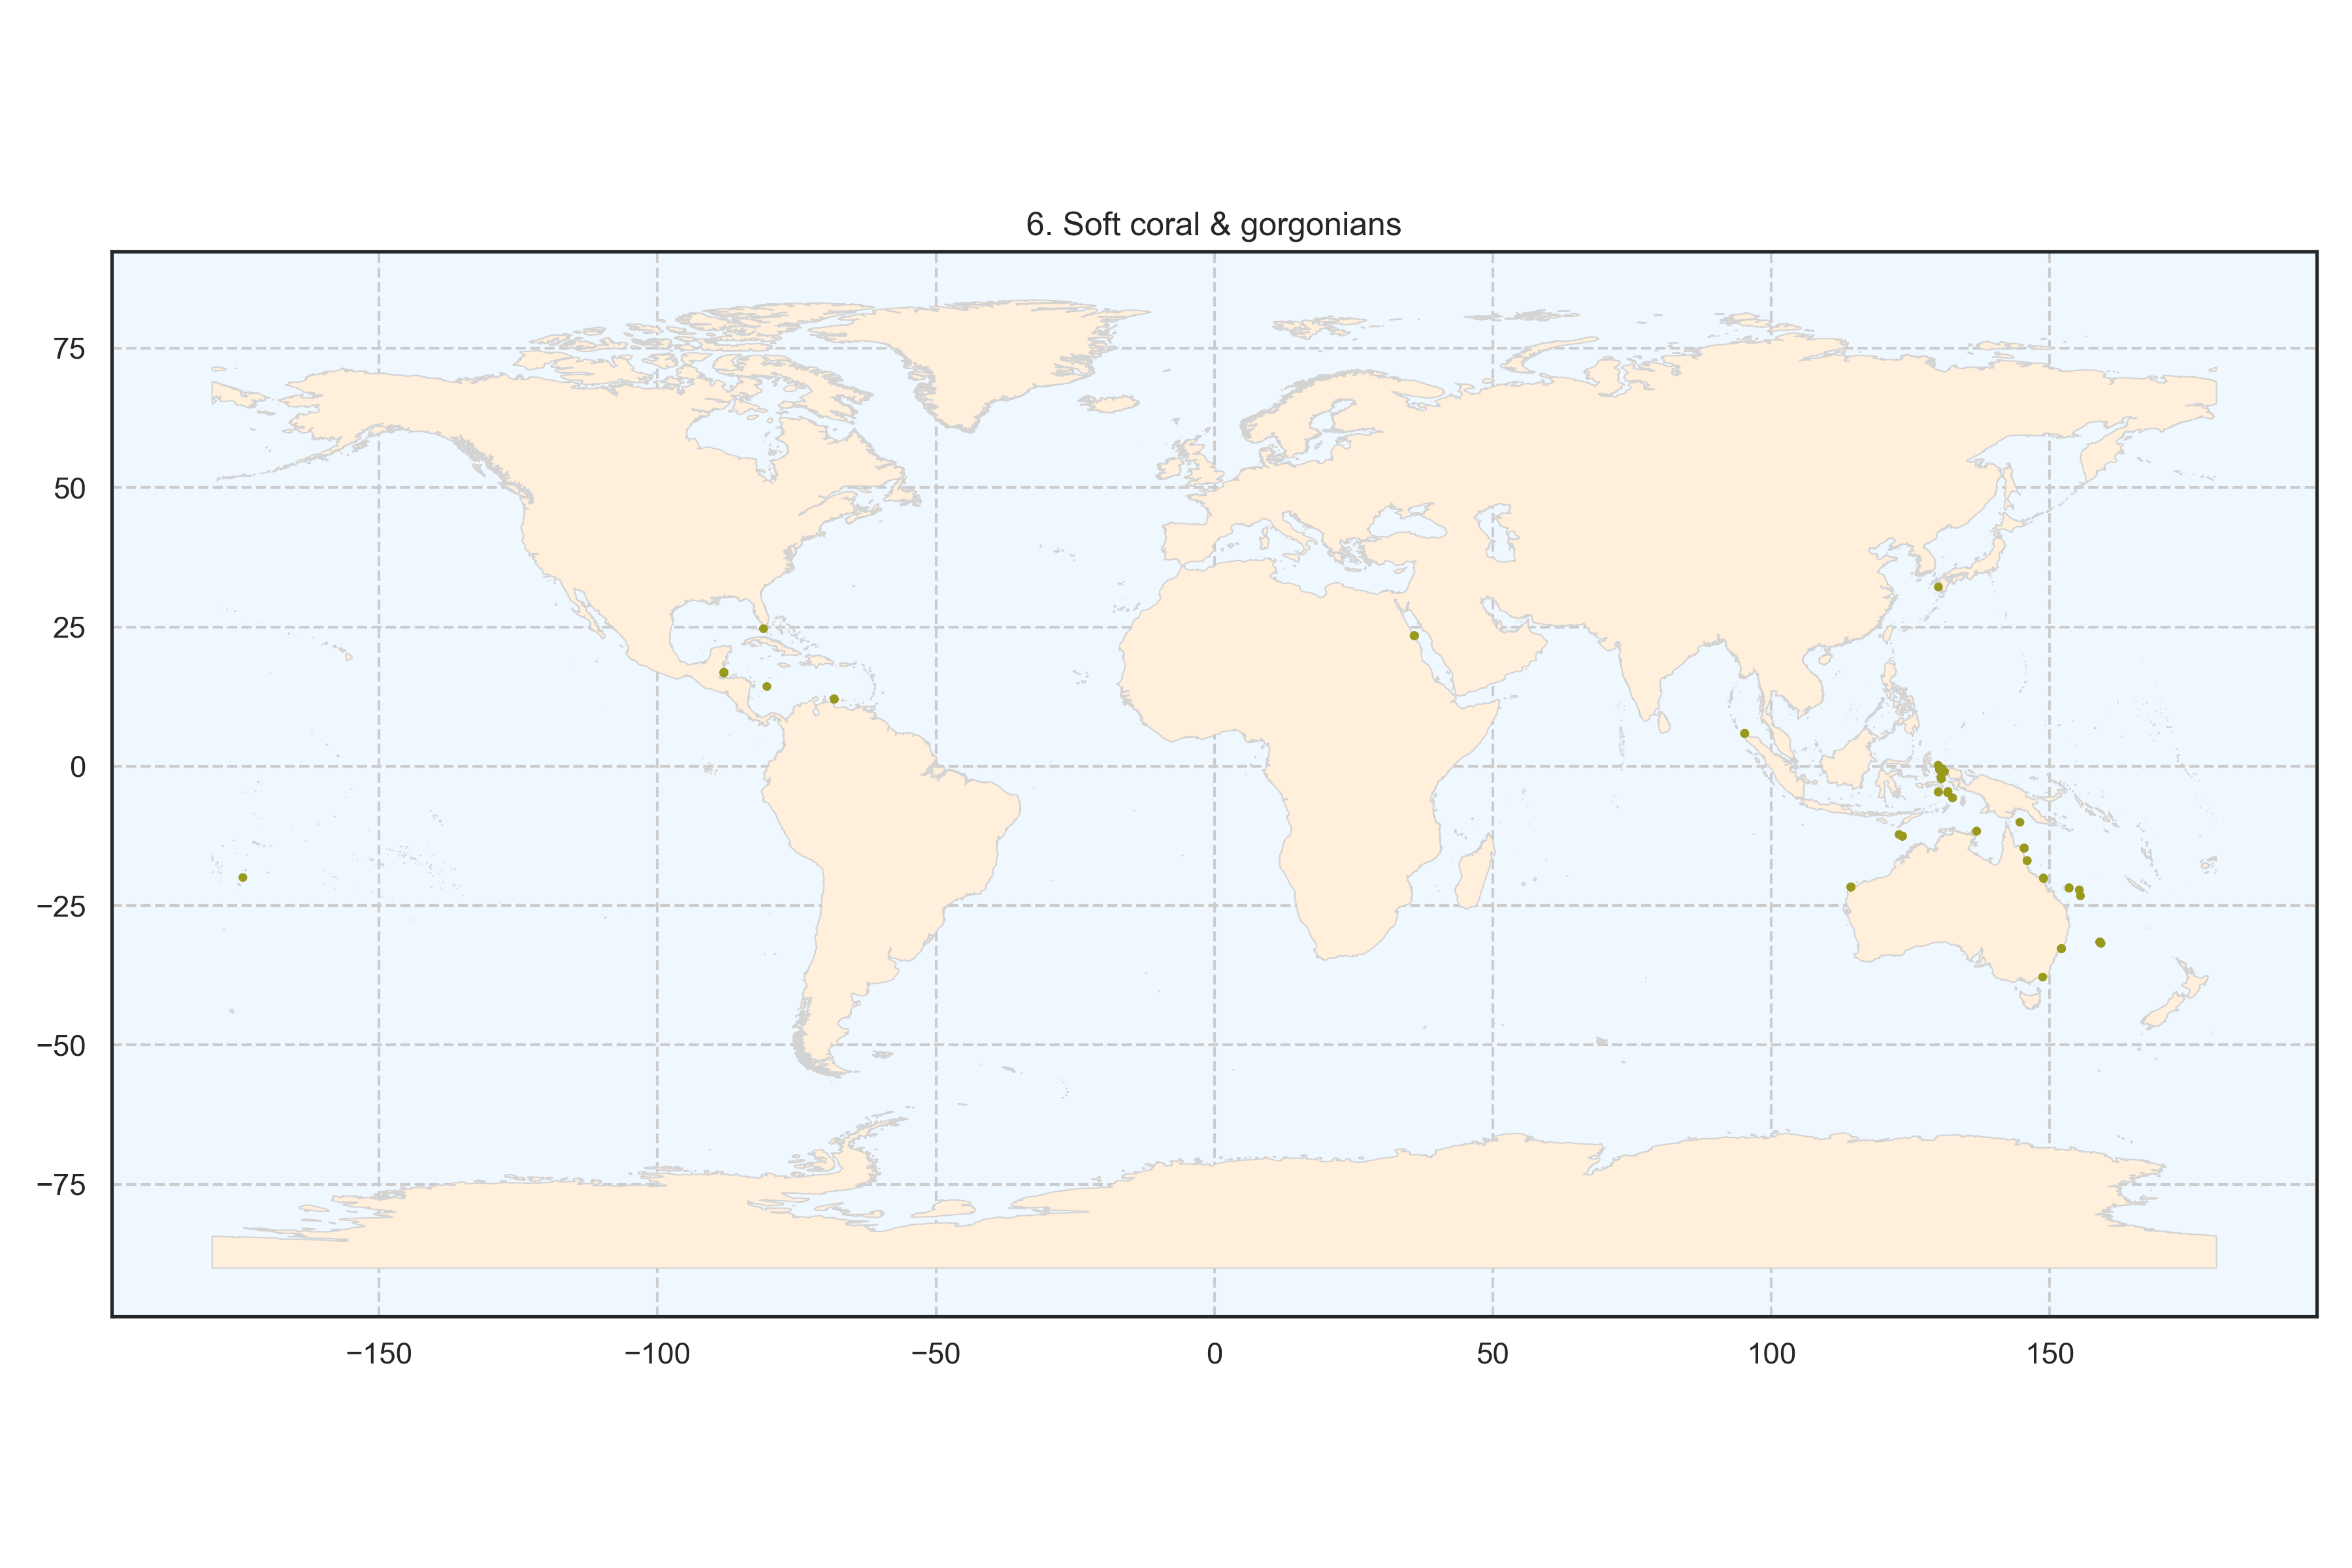
\includegraphics{03-Chapitre2/figures/supplementary/06-spatial-cluster_distribution_cluster_5.png}
\caption{Spatial distribution of the cluster \emph{soft coral and
gorgonians} at the global scale. Each point represents a
transect.}\label{fig:chap2figS8}
}
\end{figure}

\begin{figure}
\hypertarget{fig:chap2figS9}{%
\centering
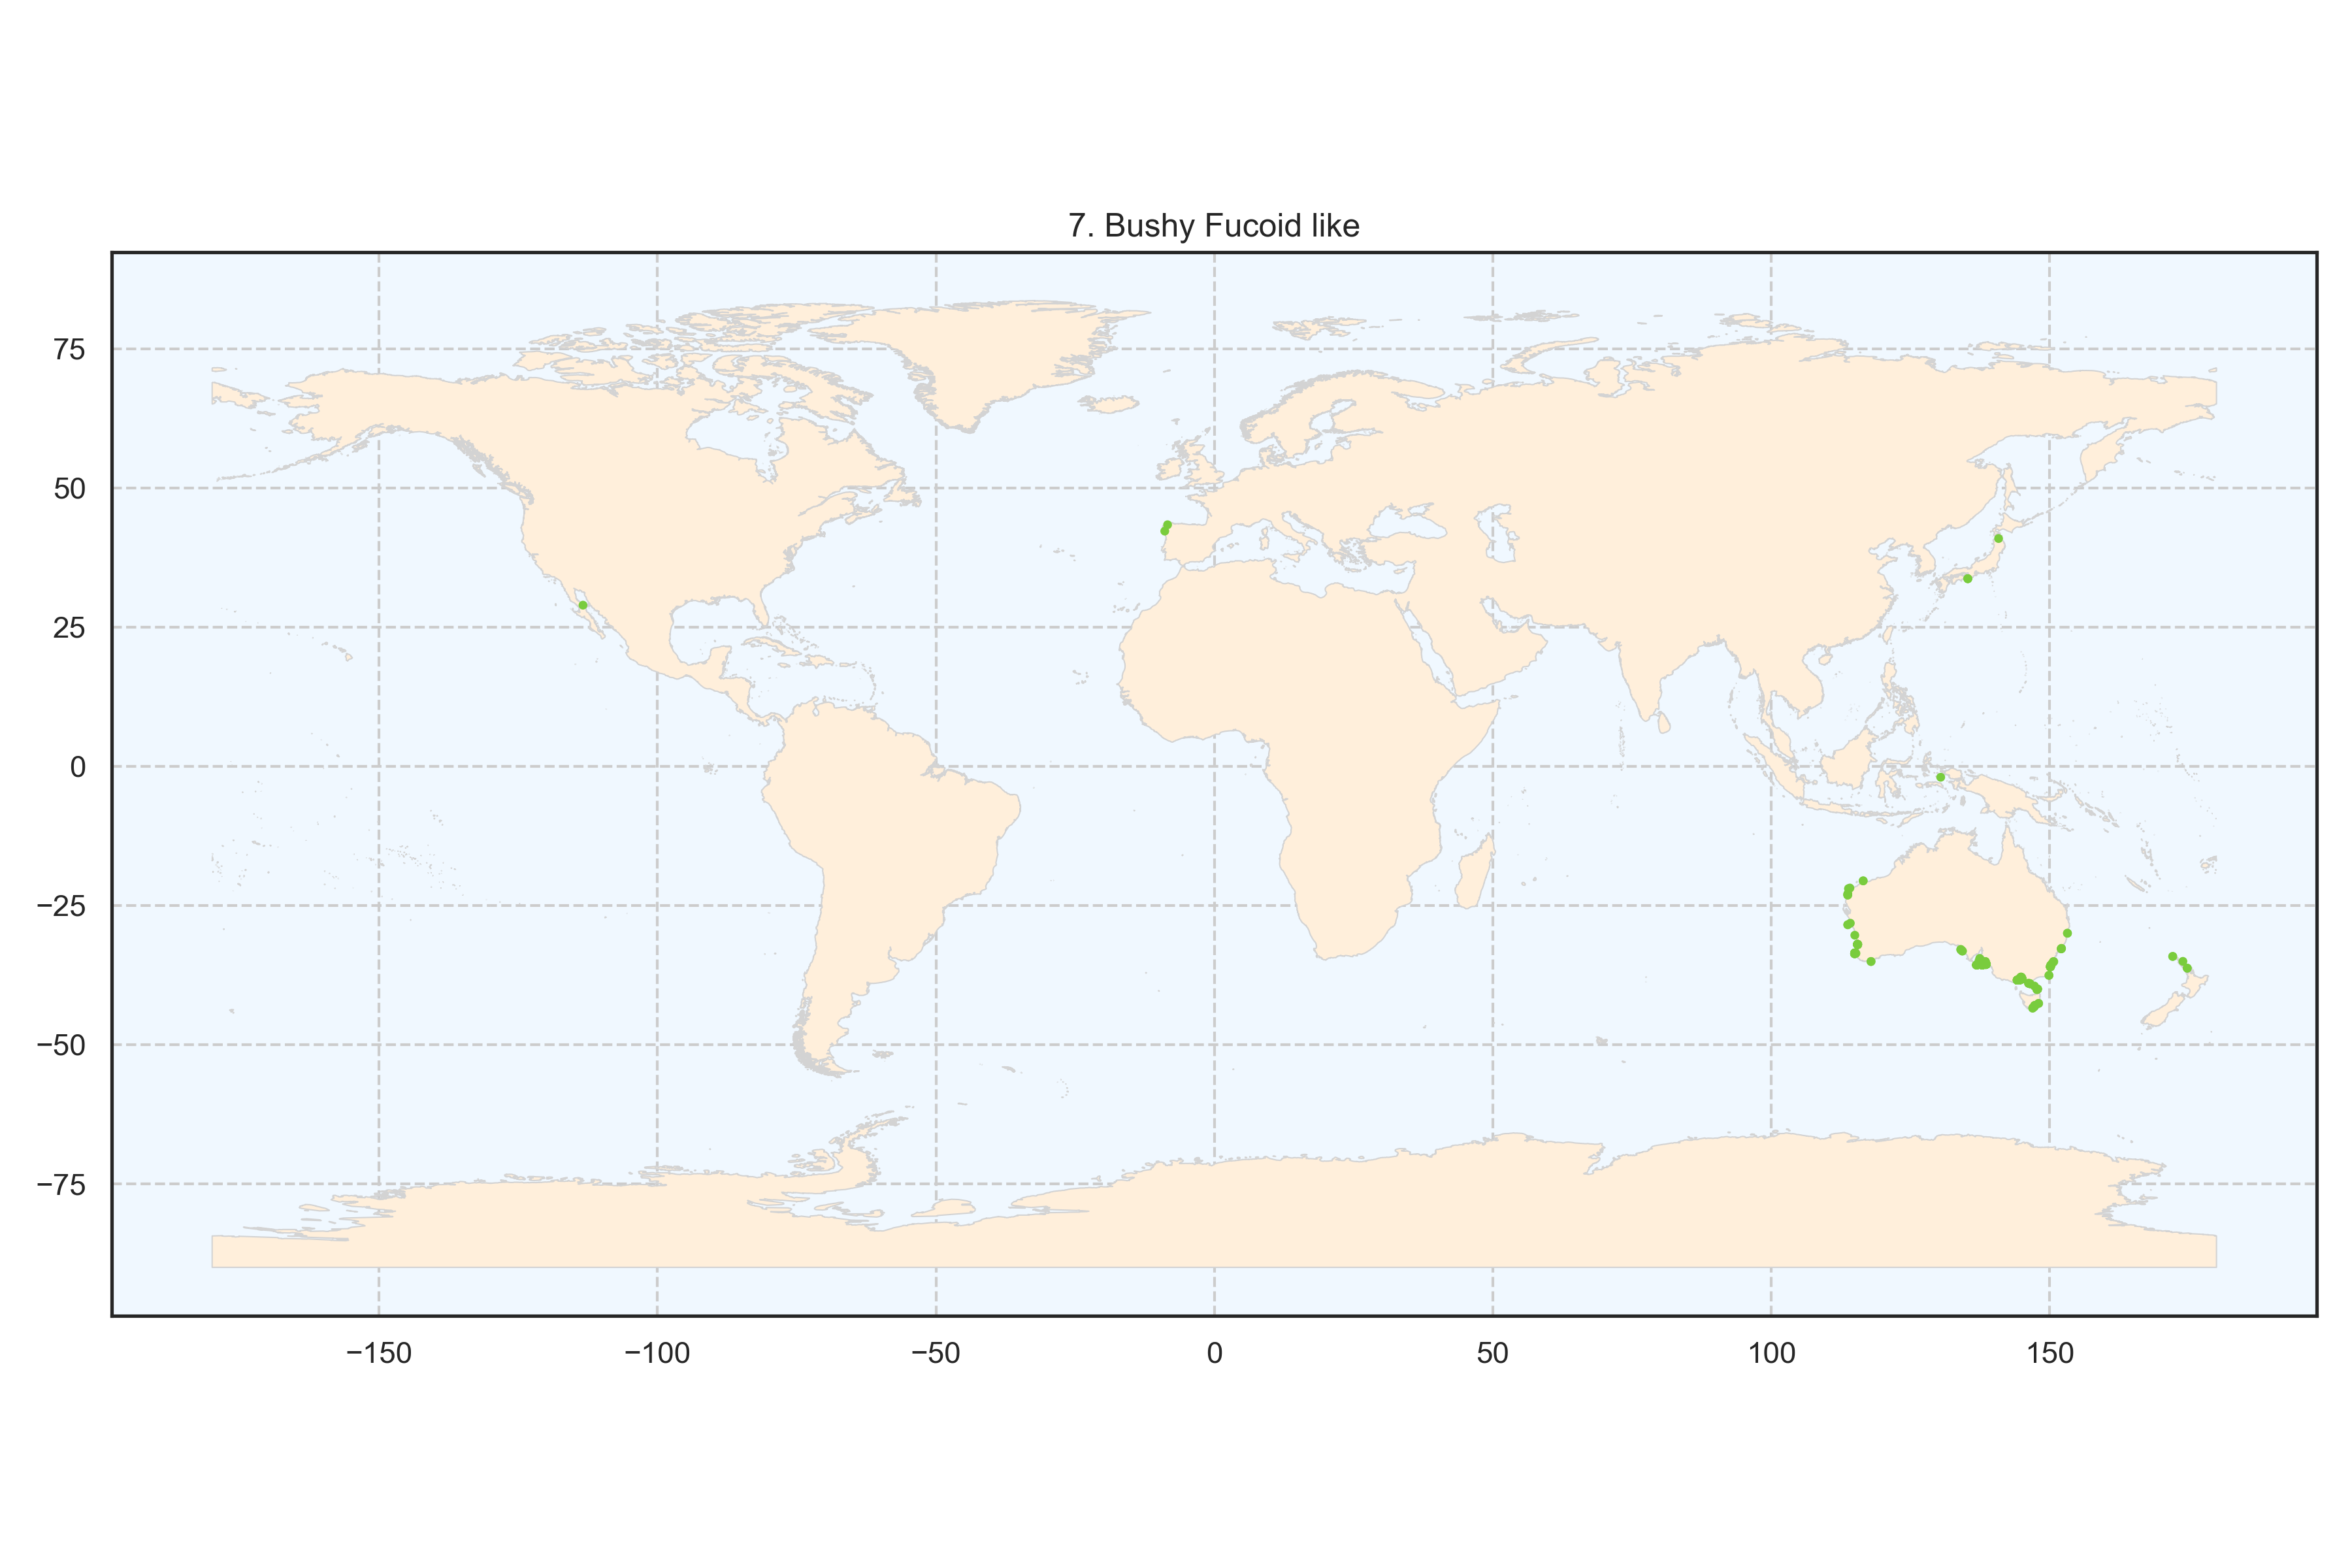
\includegraphics{03-Chapitre2/figures/supplementary/06-spatial-cluster_distribution_cluster_6.png}
\caption{Spatial distribution of the cluster \emph{bushy fucoid-like
algae} at the global scale. Each point represents a
transect.}\label{fig:chap2figS9}
}
\end{figure}

\begin{figure}
\hypertarget{fig:chap2figS10}{%
\centering
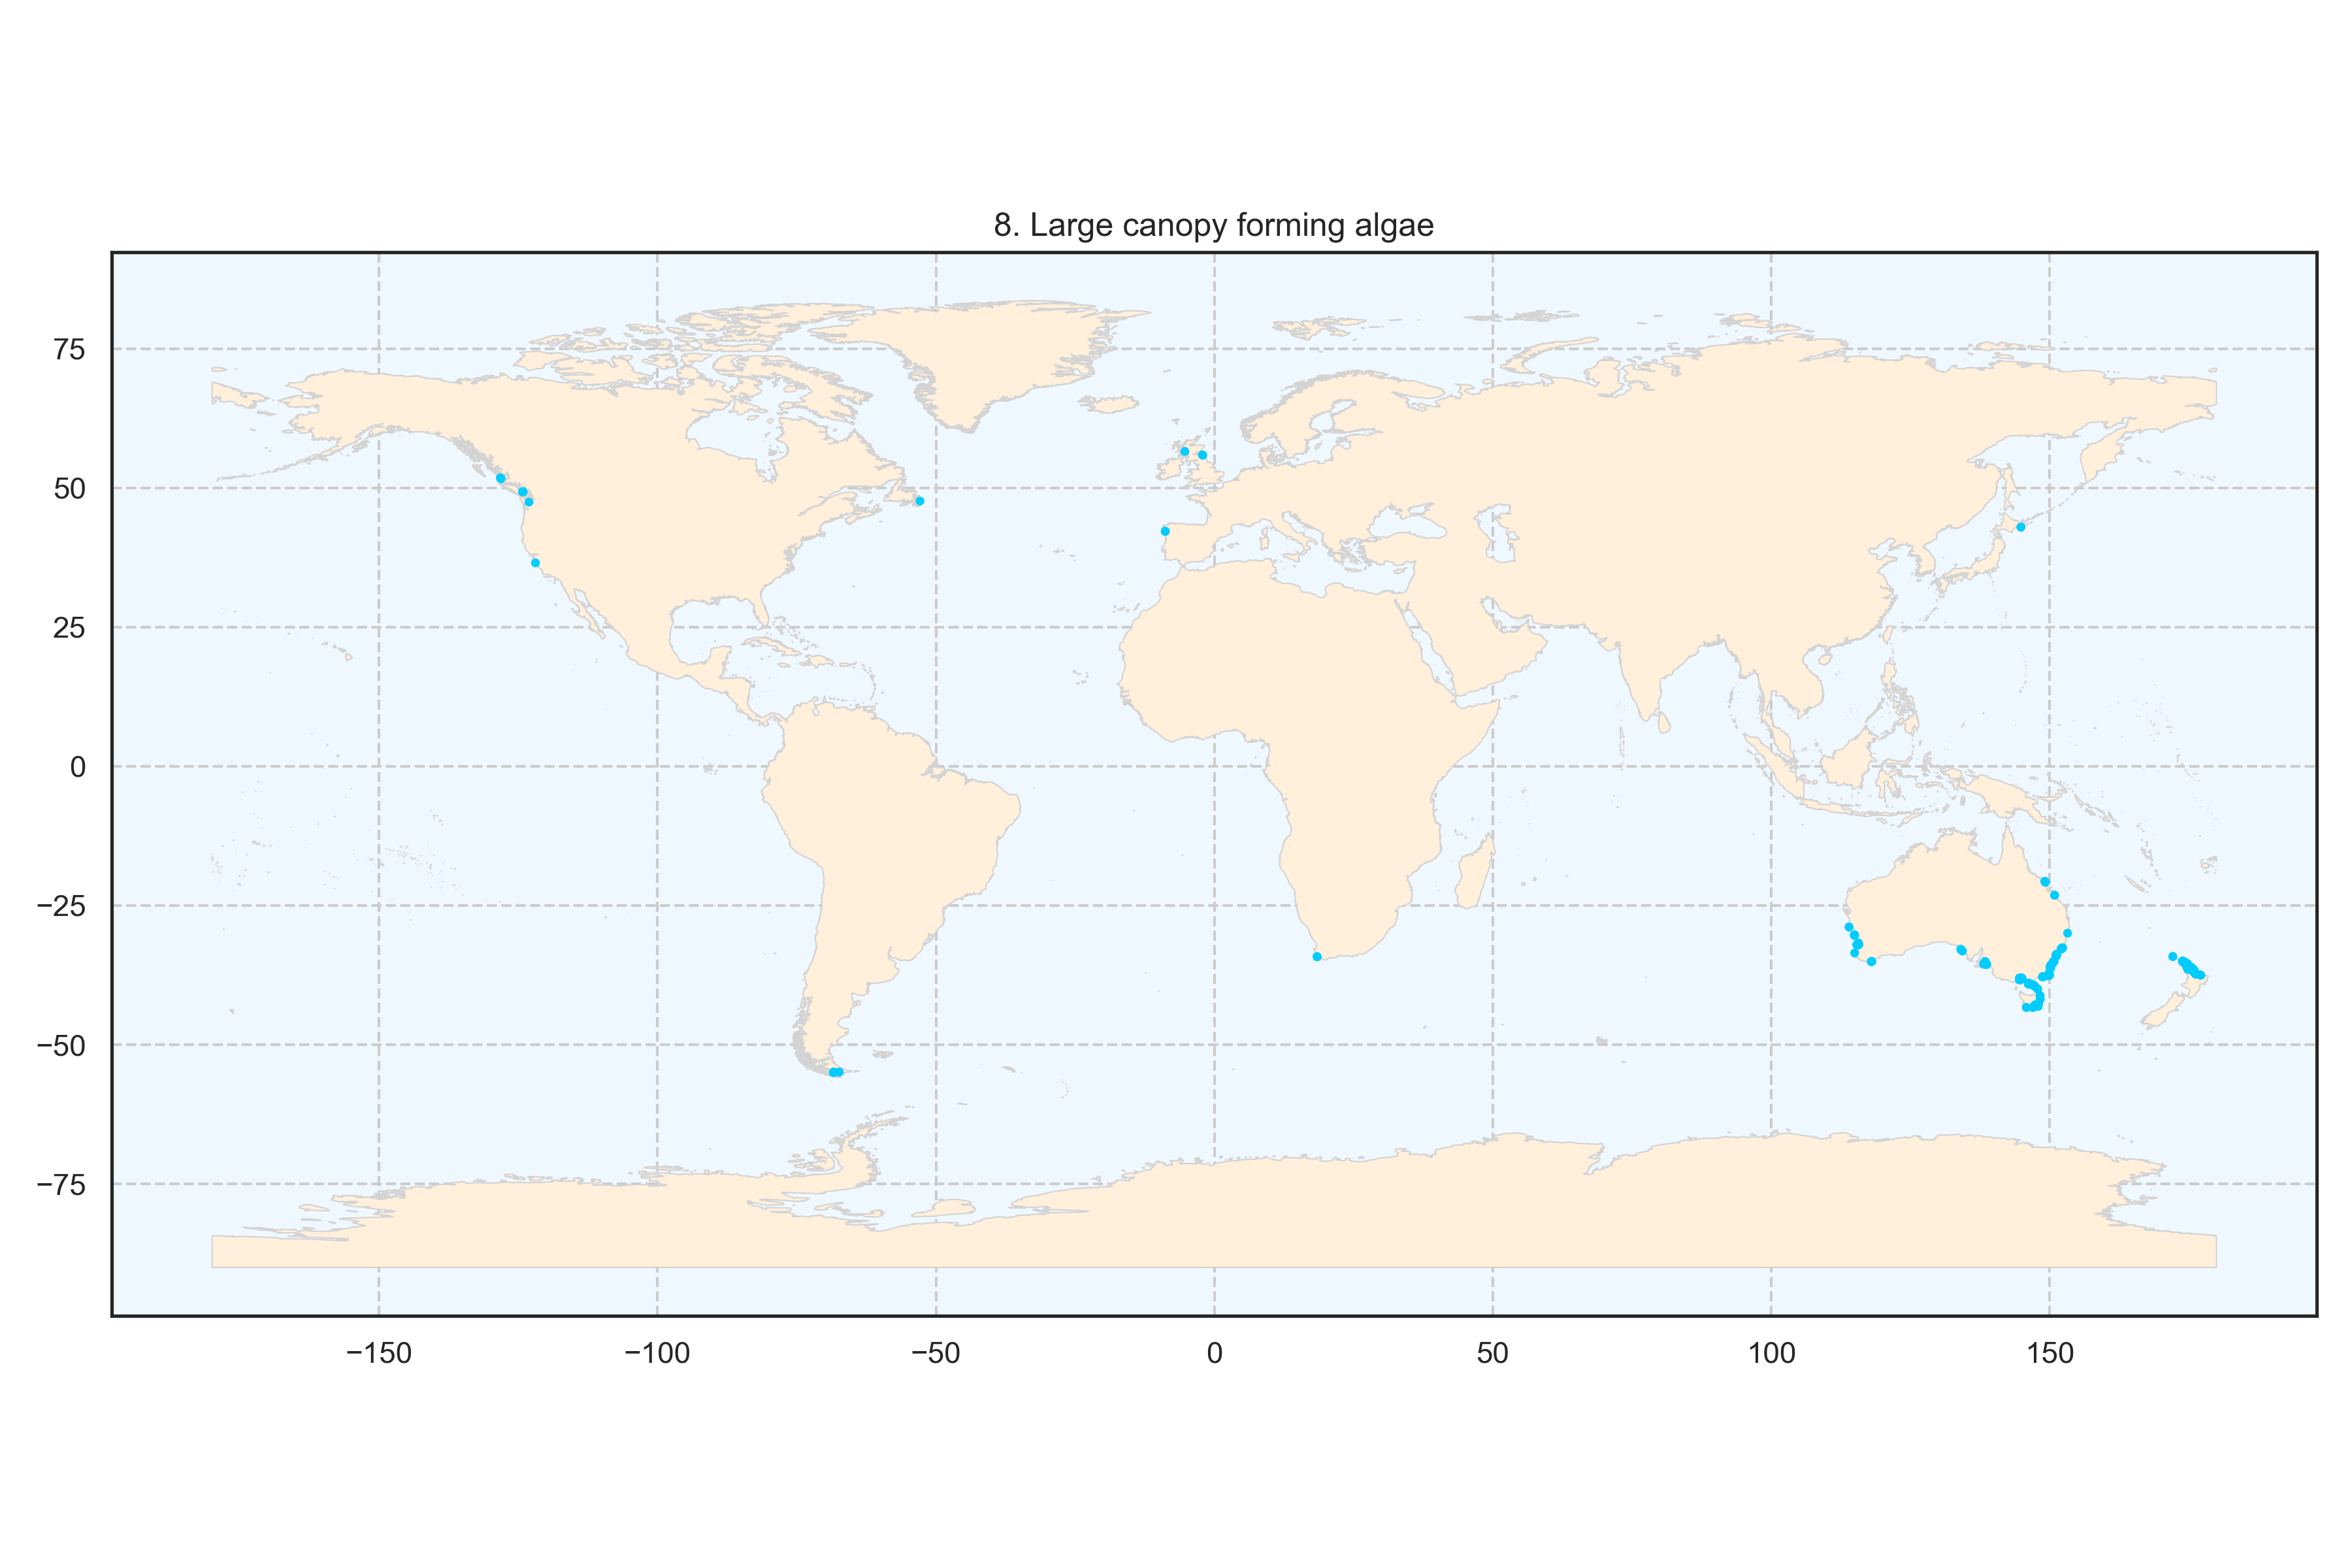
\includegraphics{03-Chapitre2/figures/supplementary/06-spatial-cluster_distribution_cluster_7.png}
\caption{Spatial distribution of the cluster \emph{large canopy forming
algae} at the global scale. Each point represents a
transect.}\label{fig:chap2figS10}
}
\end{figure}

\begin{figure}
\hypertarget{fig:chap2figS11}{%
\centering
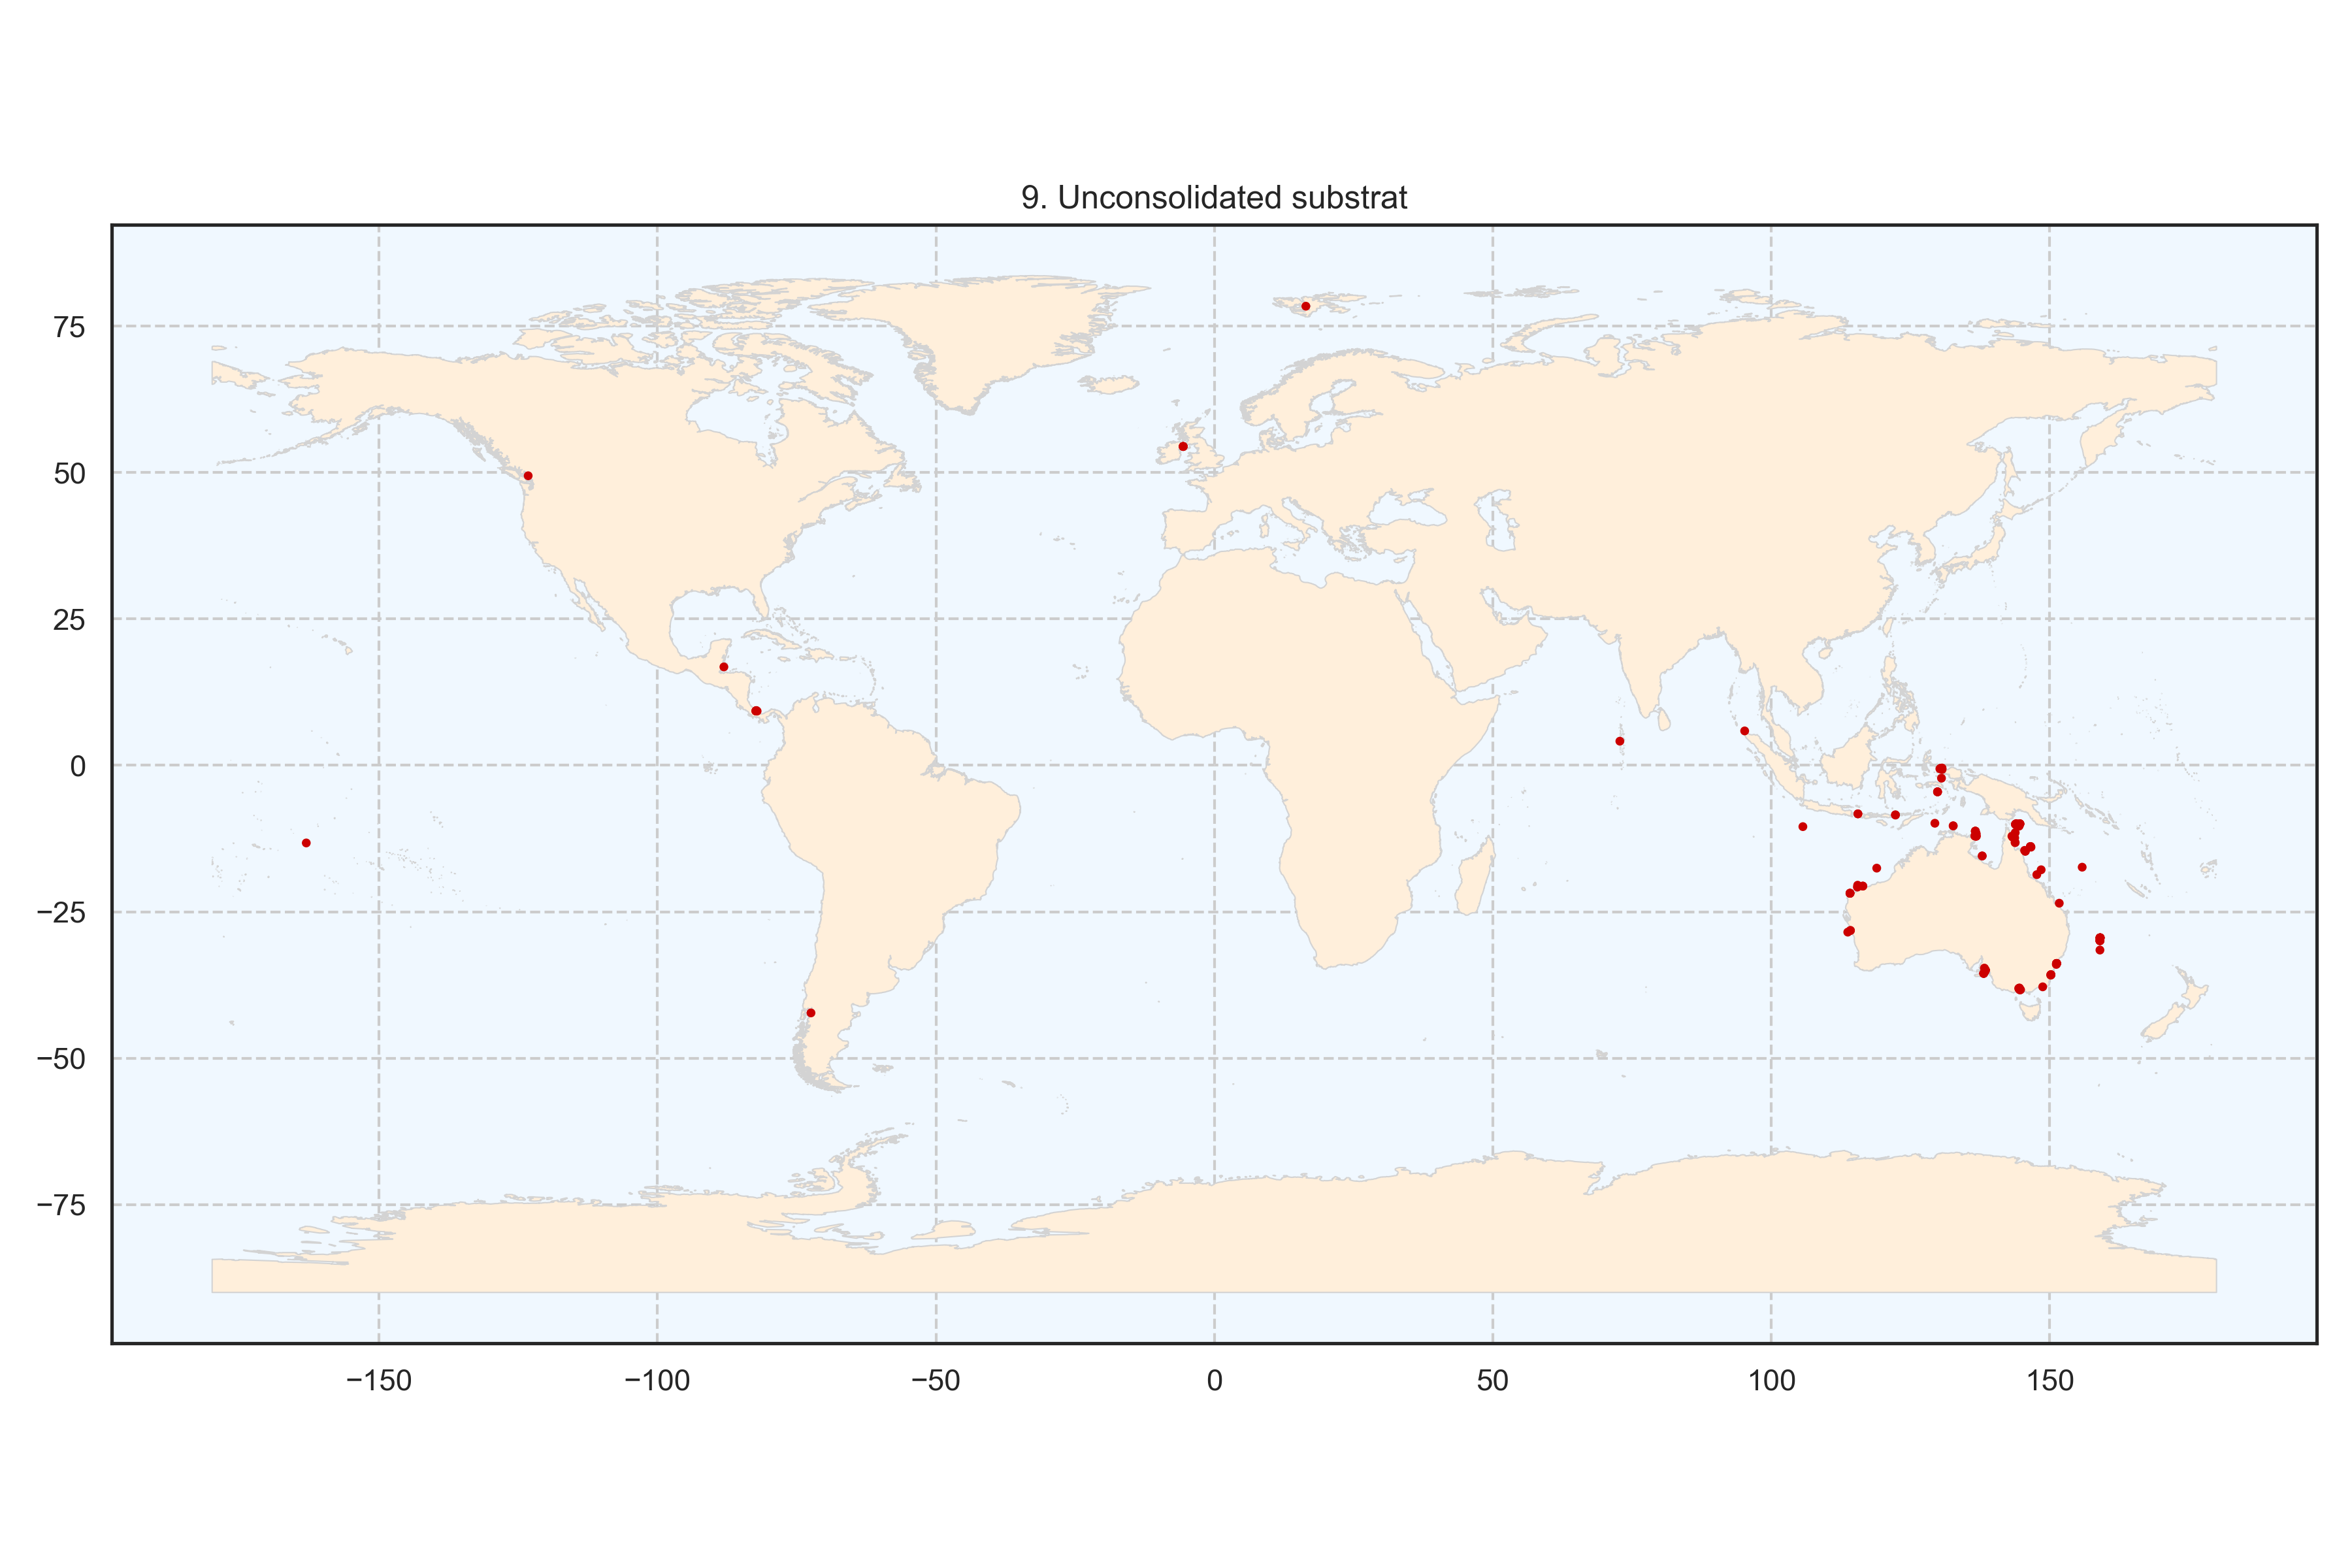
\includegraphics{03-Chapitre2/figures/supplementary/06-spatial-cluster_distribution_cluster_8.png}
\caption{Spatial distribution of the cluster \emph{unconsolidated
substrate} at the global scale. Each point represents a
transect.}\label{fig:chap2figS11}
}
\end{figure}

\begin{figure}
\hypertarget{fig:chap2figS12}{%
\centering
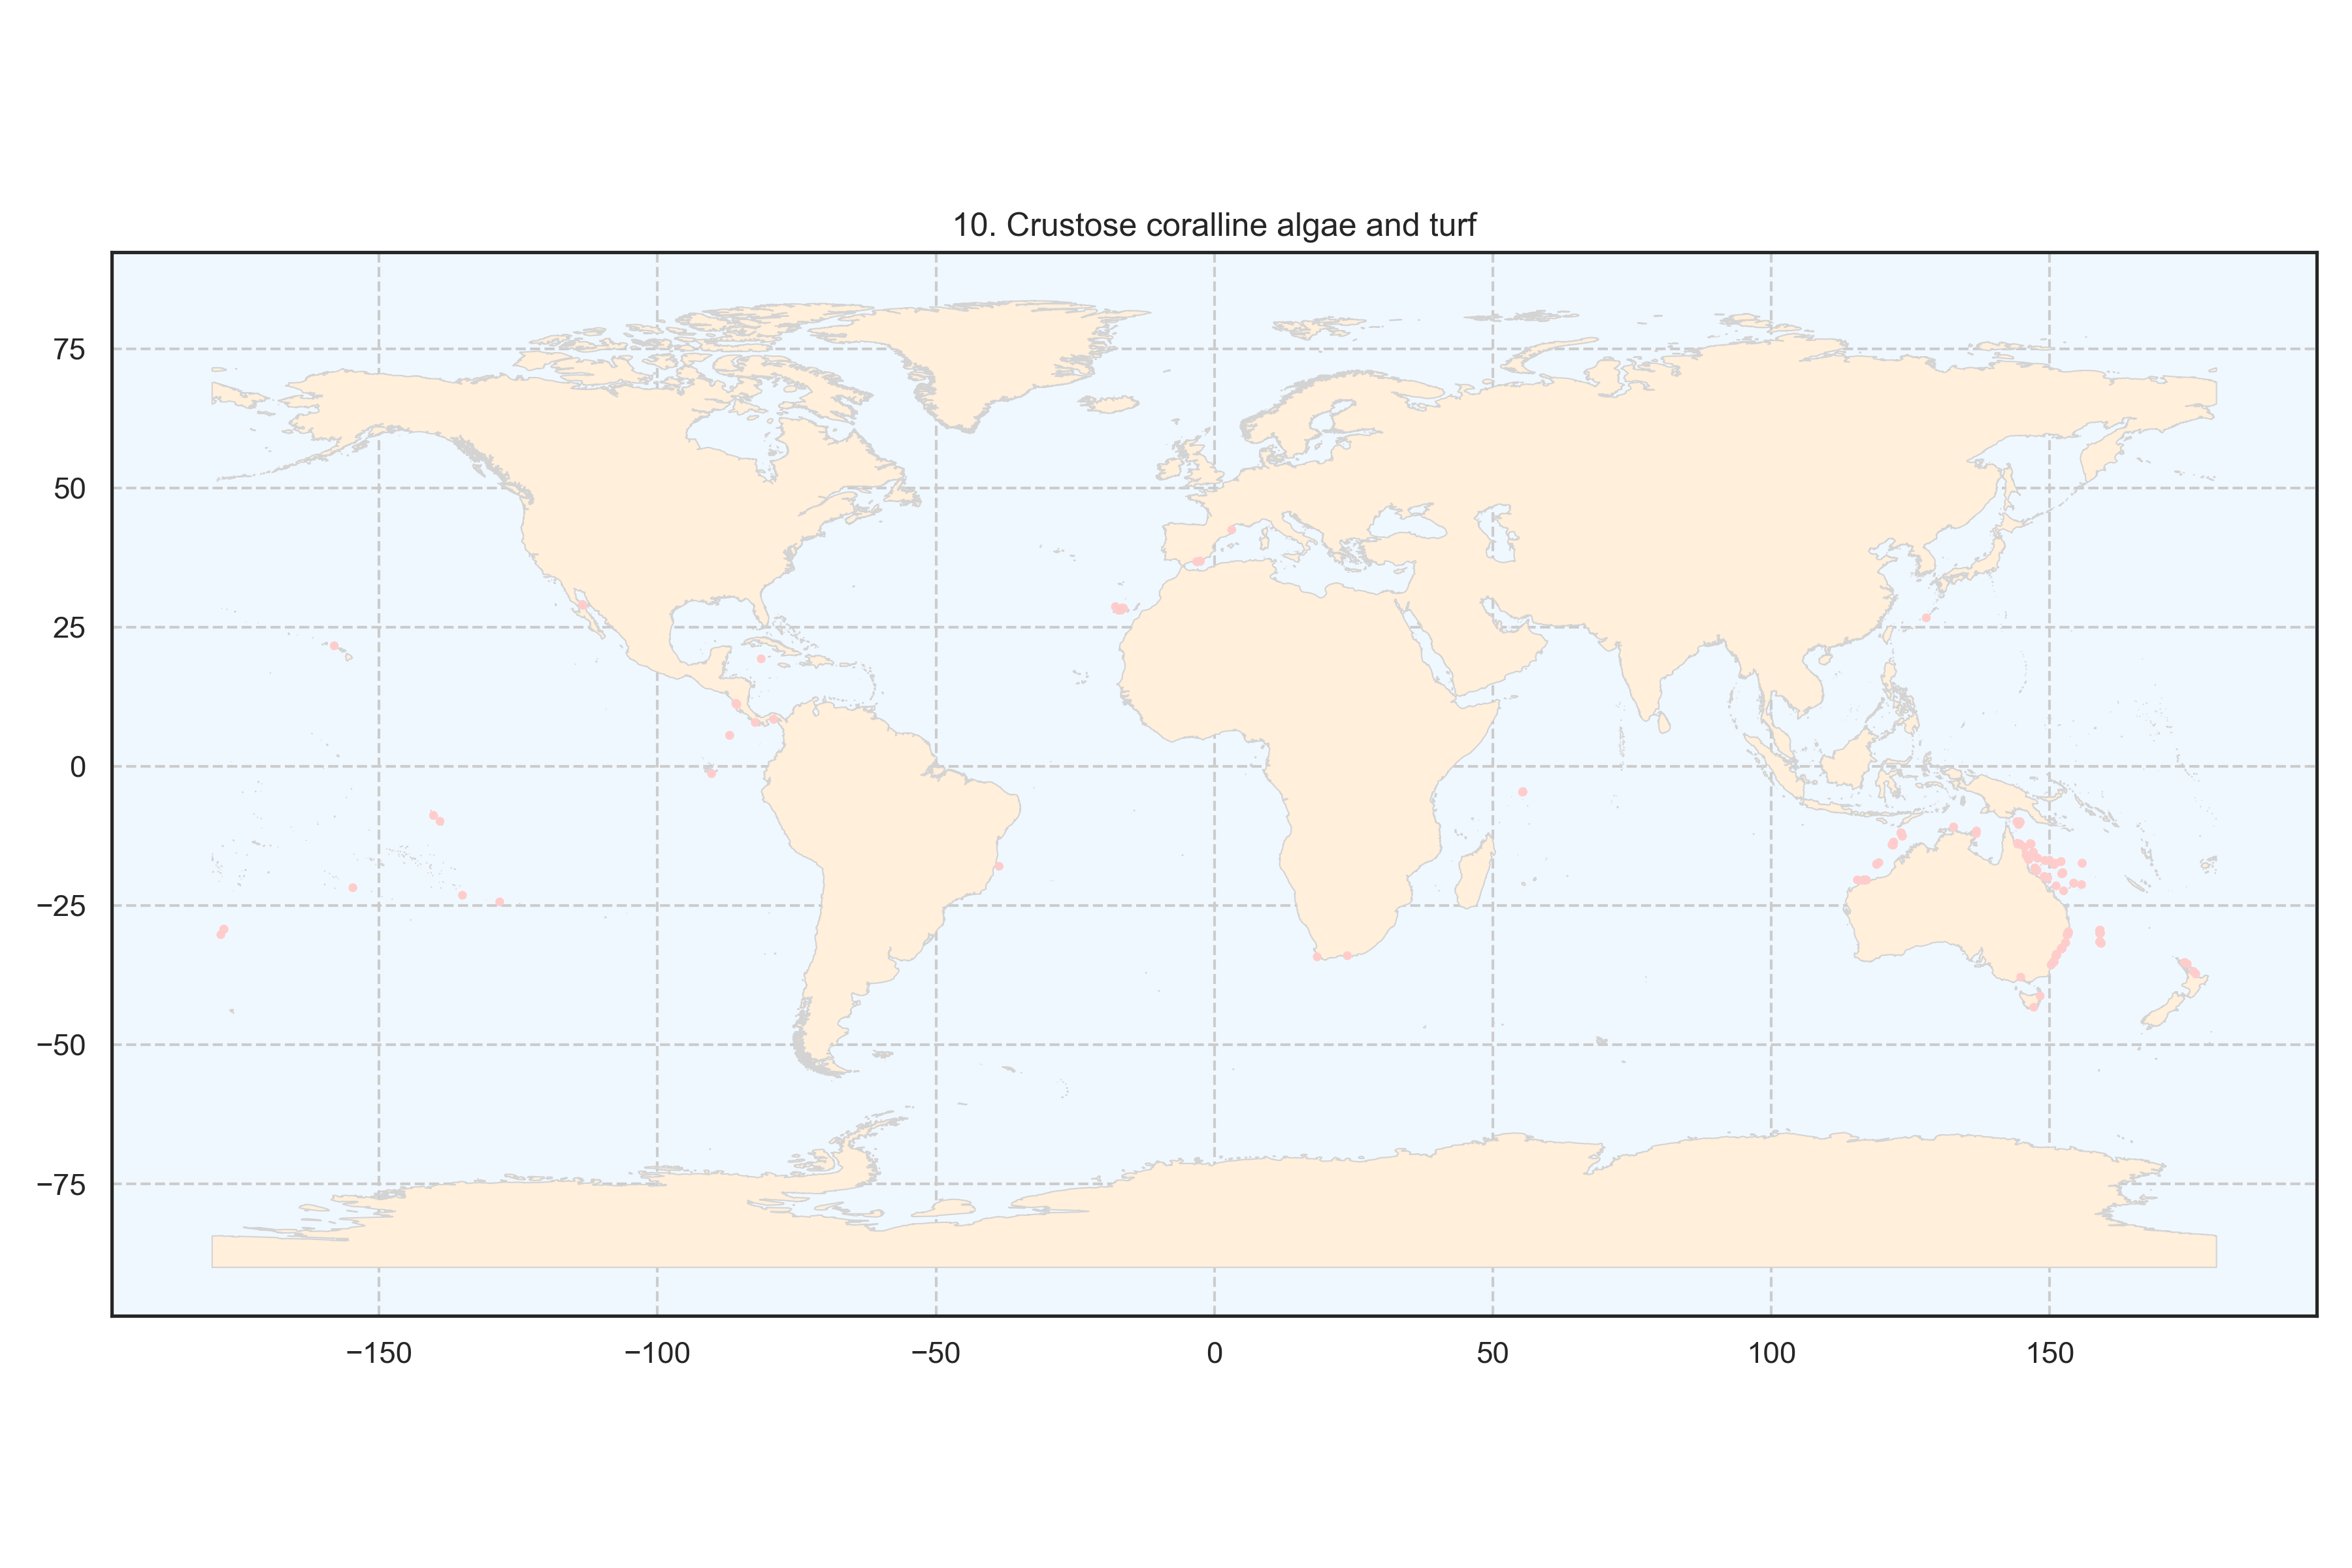
\includegraphics{03-Chapitre2/figures/supplementary/06-spatial-cluster_distribution_cluster_9.png}
\caption{Spatial distribution of the cluster \emph{crustose coralline
algae and turf} at the global scale. Each point represents a
transect.}\label{fig:chap2figS12}
}
\end{figure}

\begin{figure}
\hypertarget{fig:chap2figS13}{%
\centering
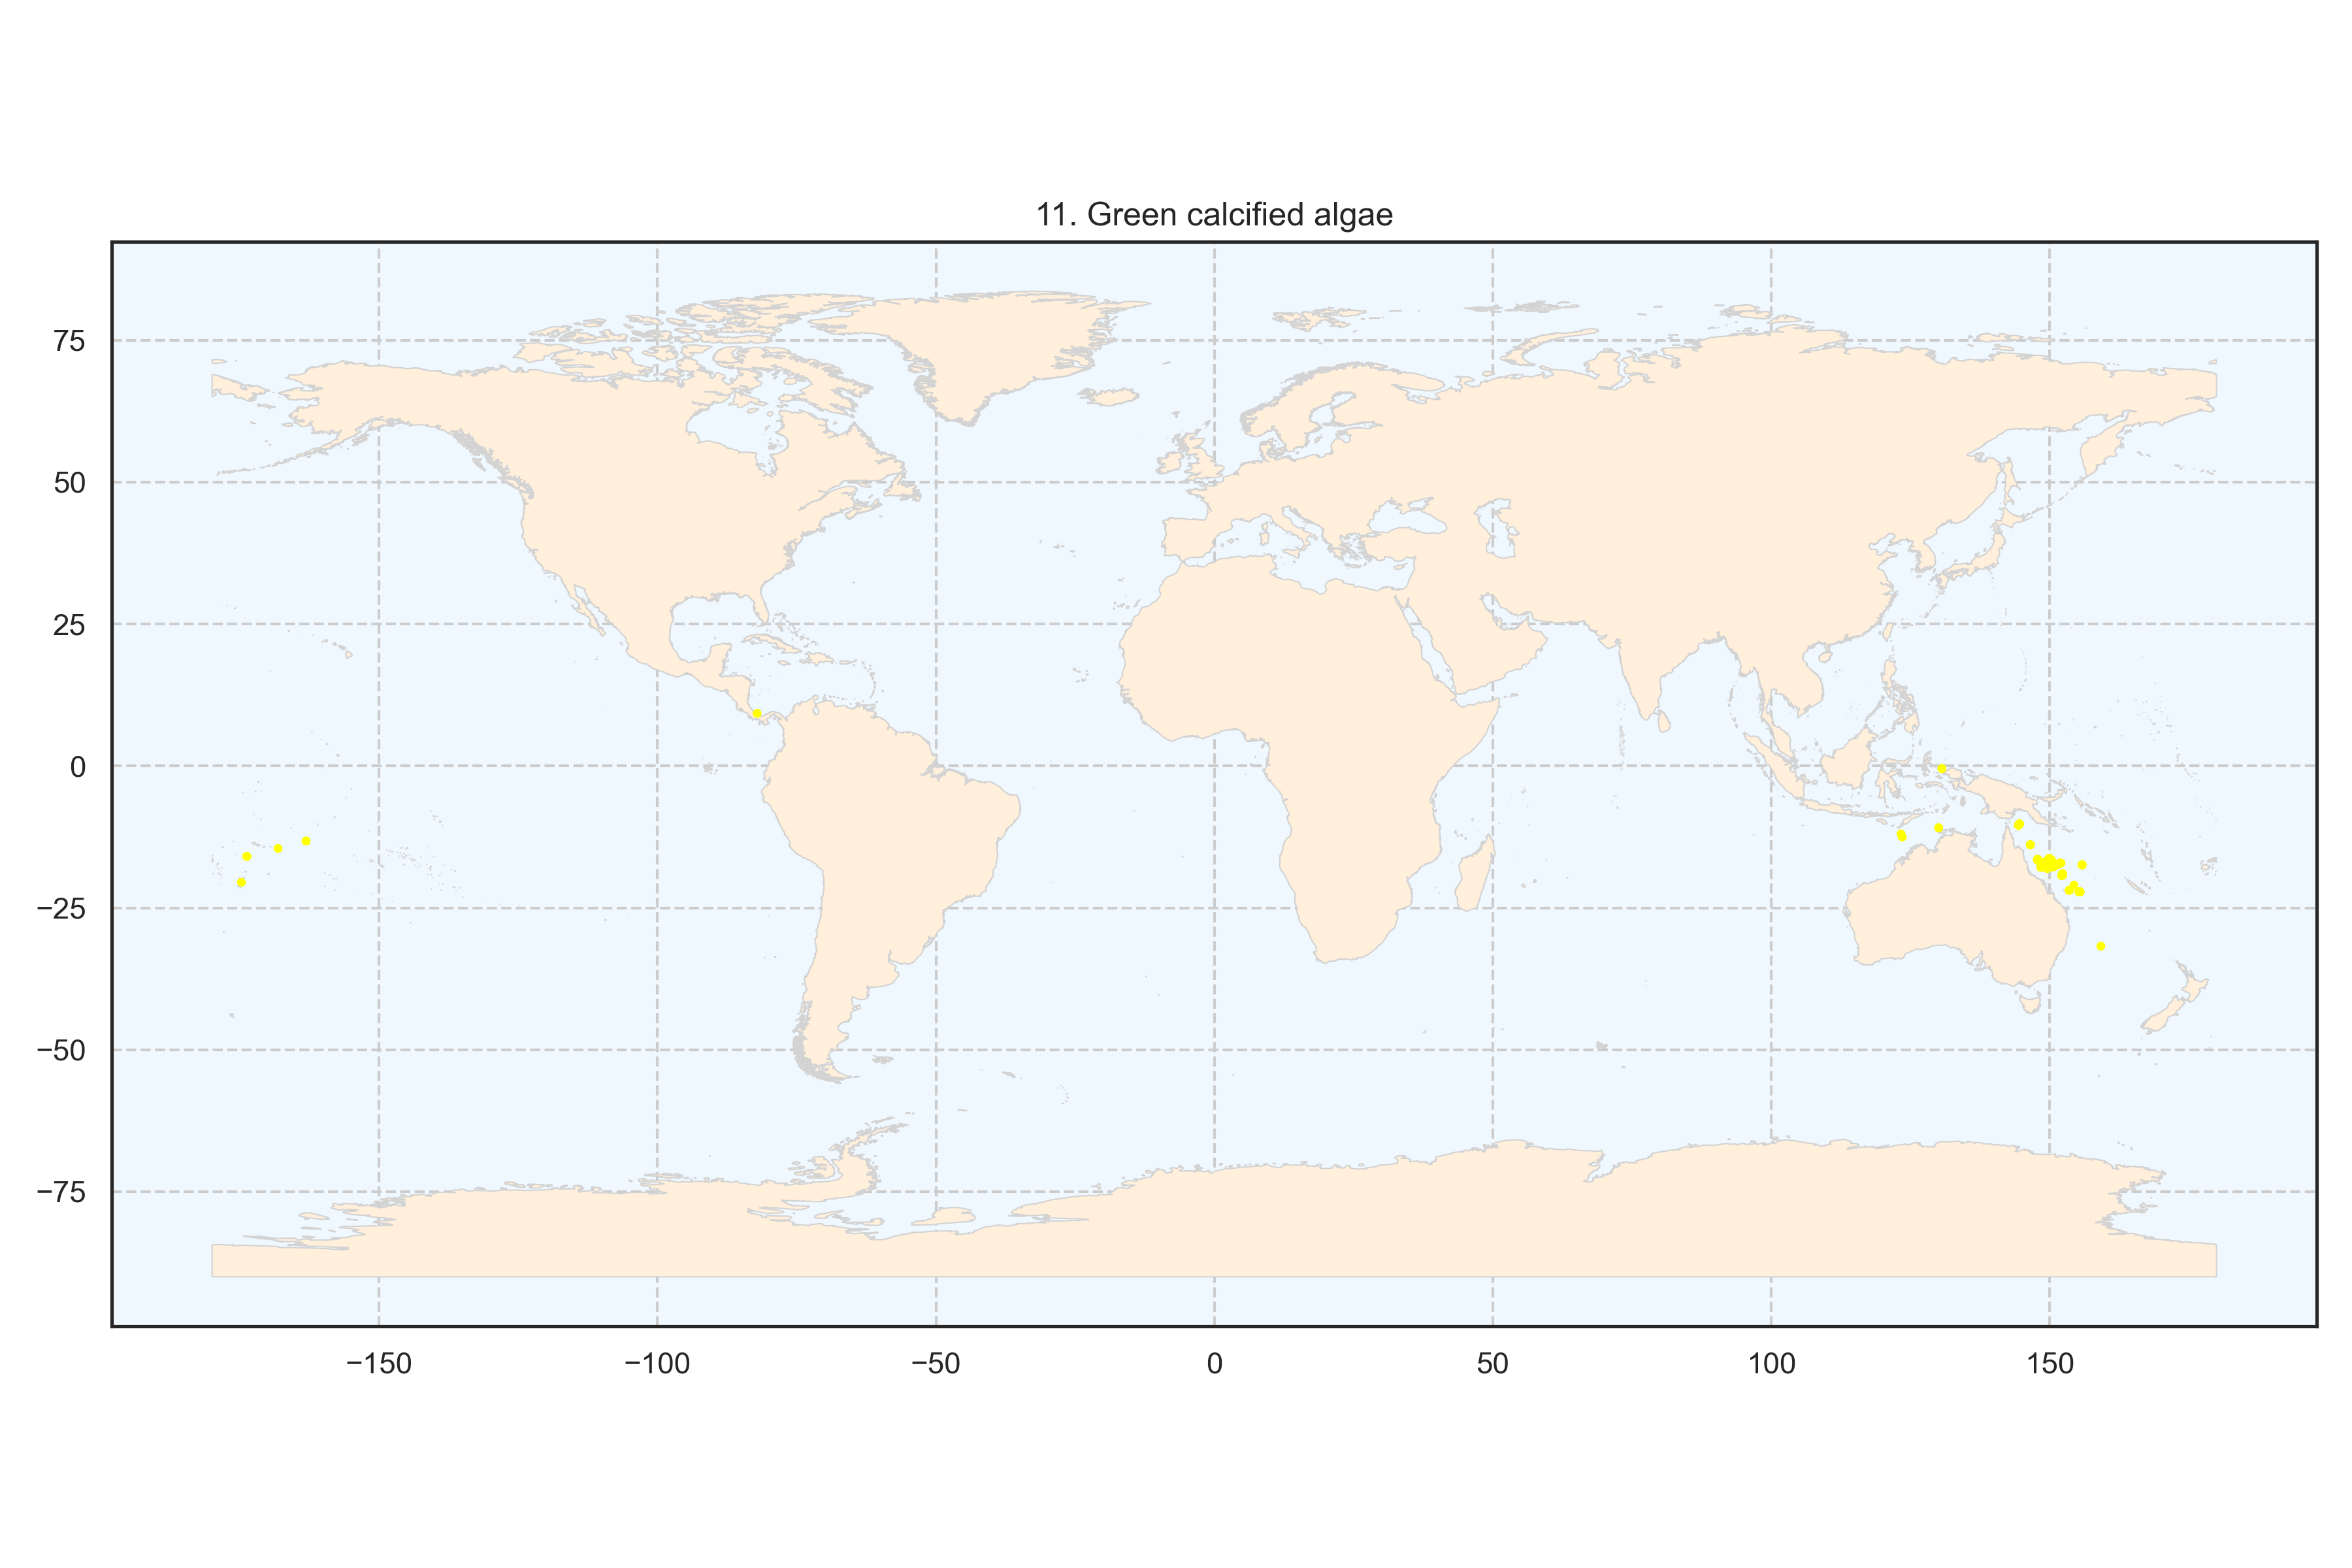
\includegraphics{03-Chapitre2/figures/supplementary/06-spatial-cluster_distribution_cluster_10.png}
\caption{Spatial distribution of the cluster \emph{green calcified
algae} at the global scale. Each point represents a
transect.}\label{fig:chap2figS13}
}
\end{figure}

\begin{figure}
\hypertarget{fig:chap2figS14}{%
\centering
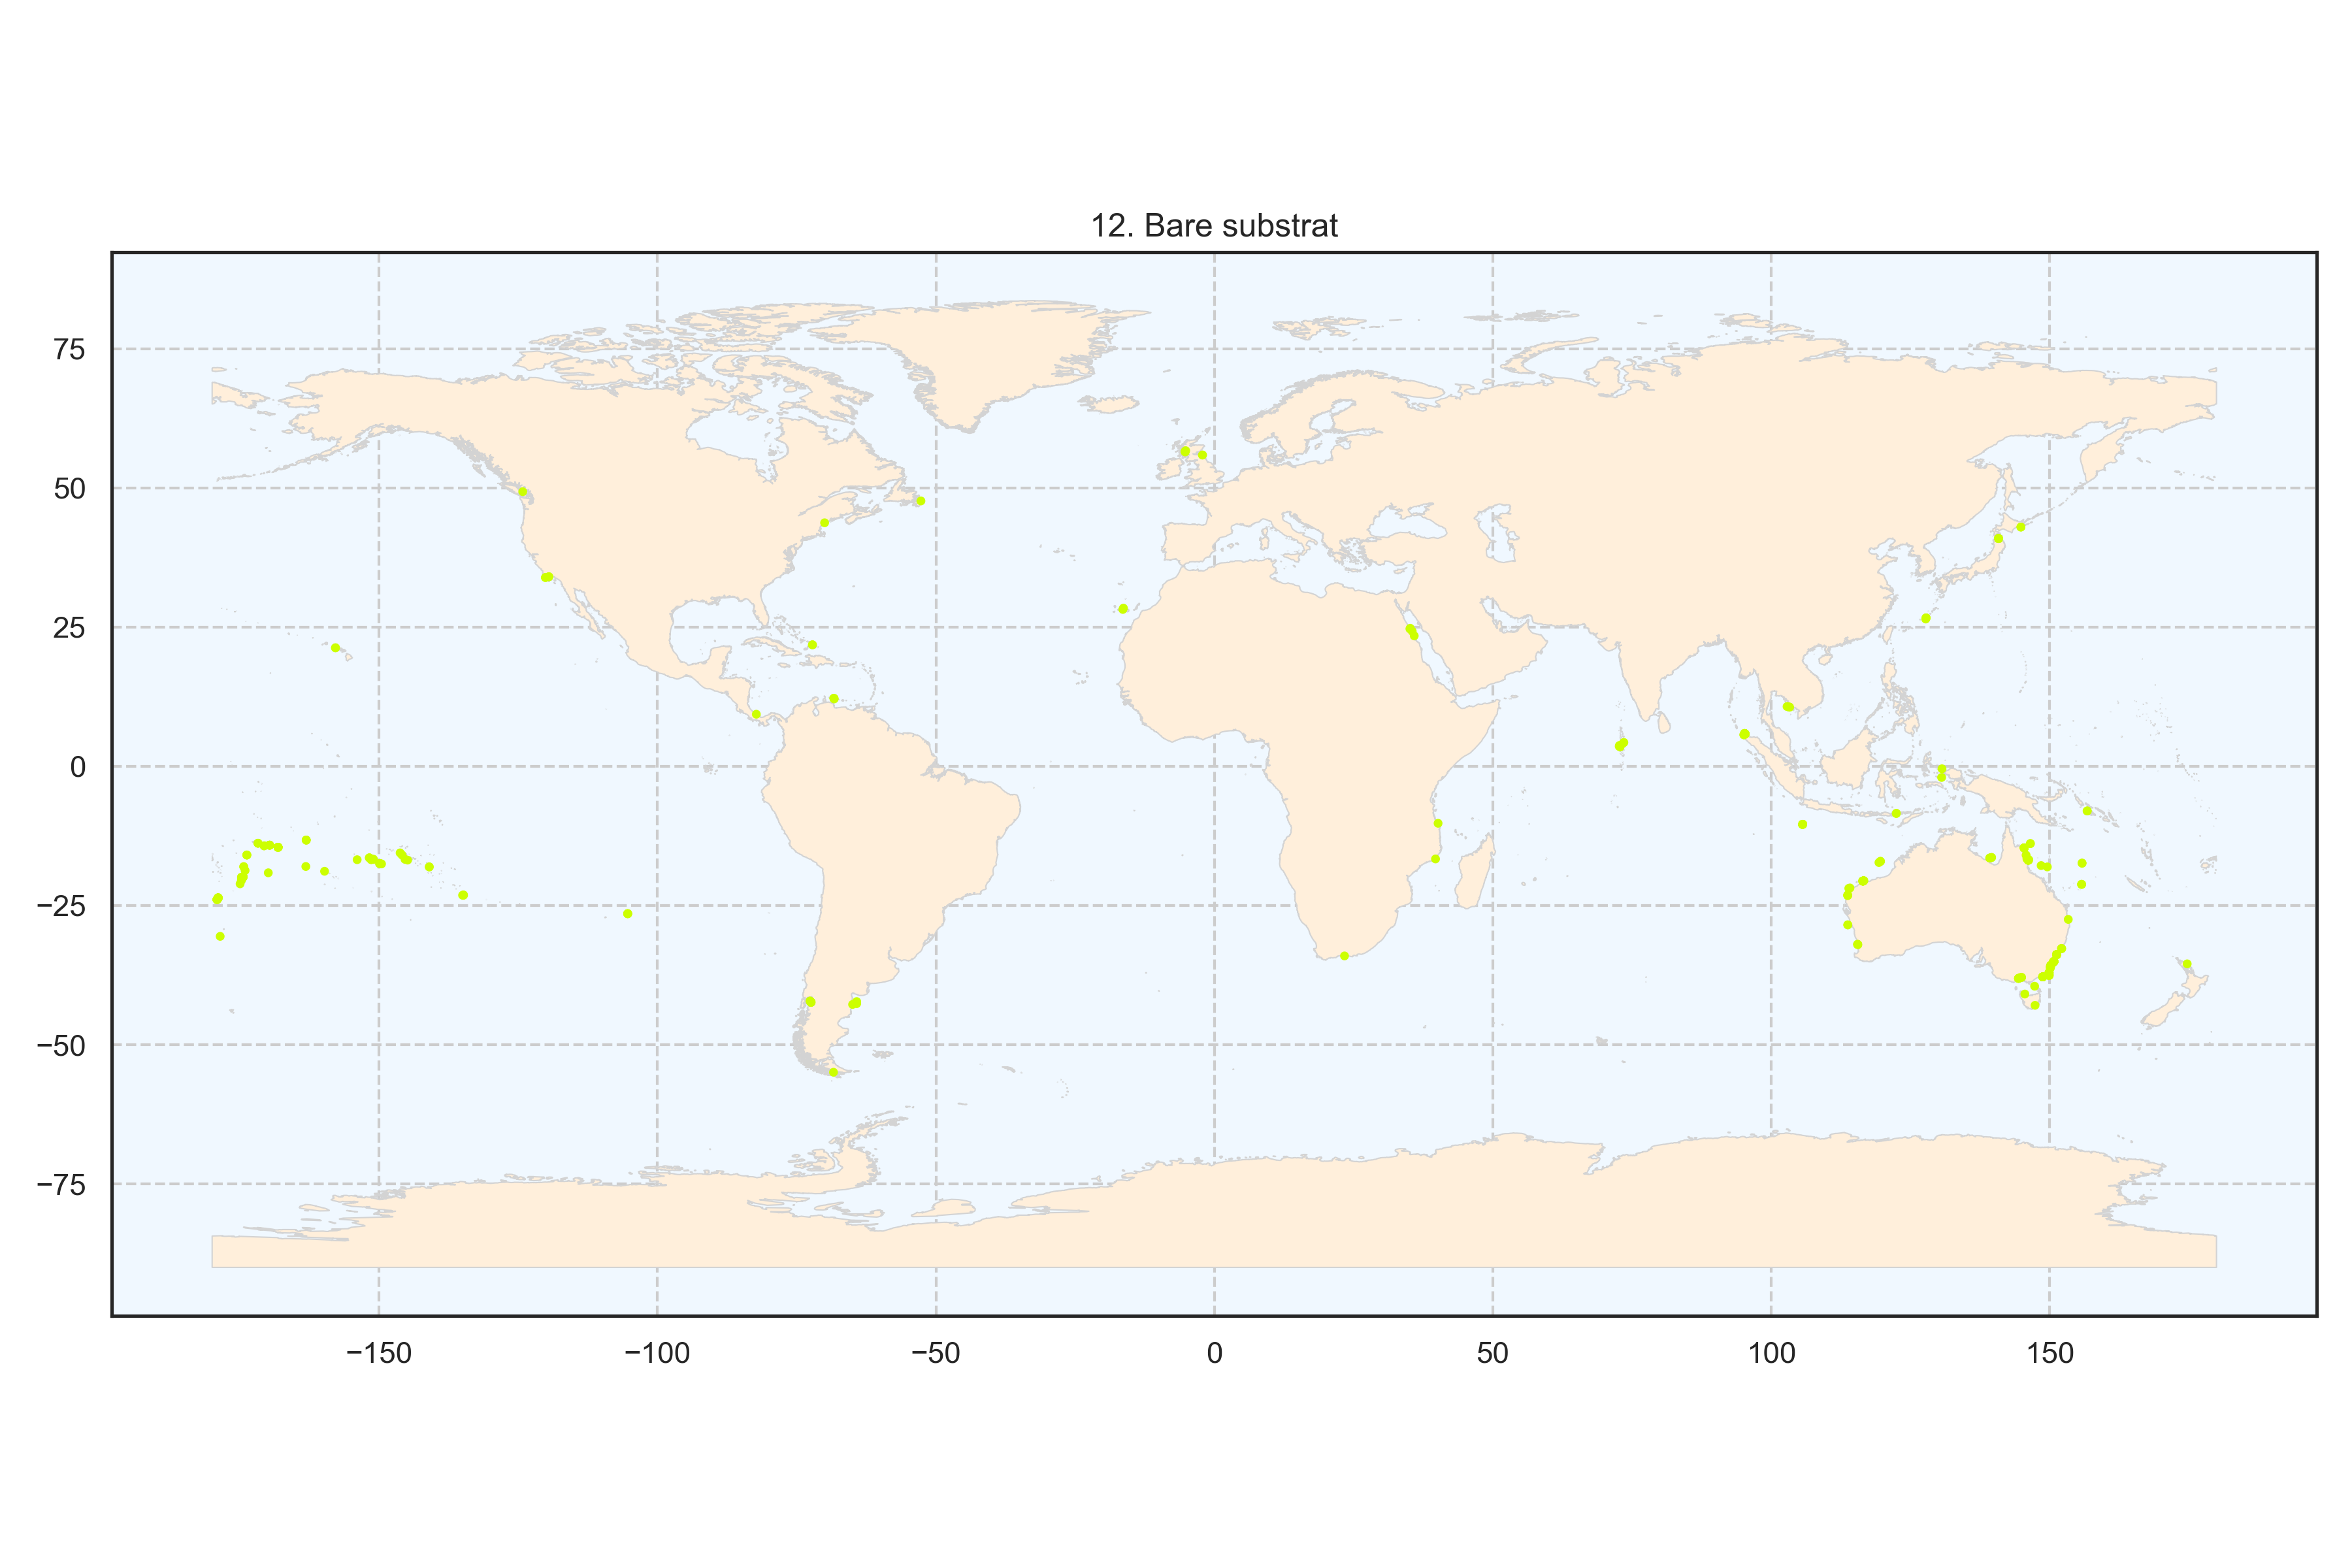
\includegraphics{03-Chapitre2/figures/supplementary/06-spatial-cluster_distribution_cluster_11.png}
\caption{Spatial distribution of the cluster \emph{bare substrate} at
the global scale. Each point represents a
transect.}\label{fig:chap2figS14}
}
\end{figure}

\begin{figure}
\hypertarget{fig:chap2figS15}{%
\centering
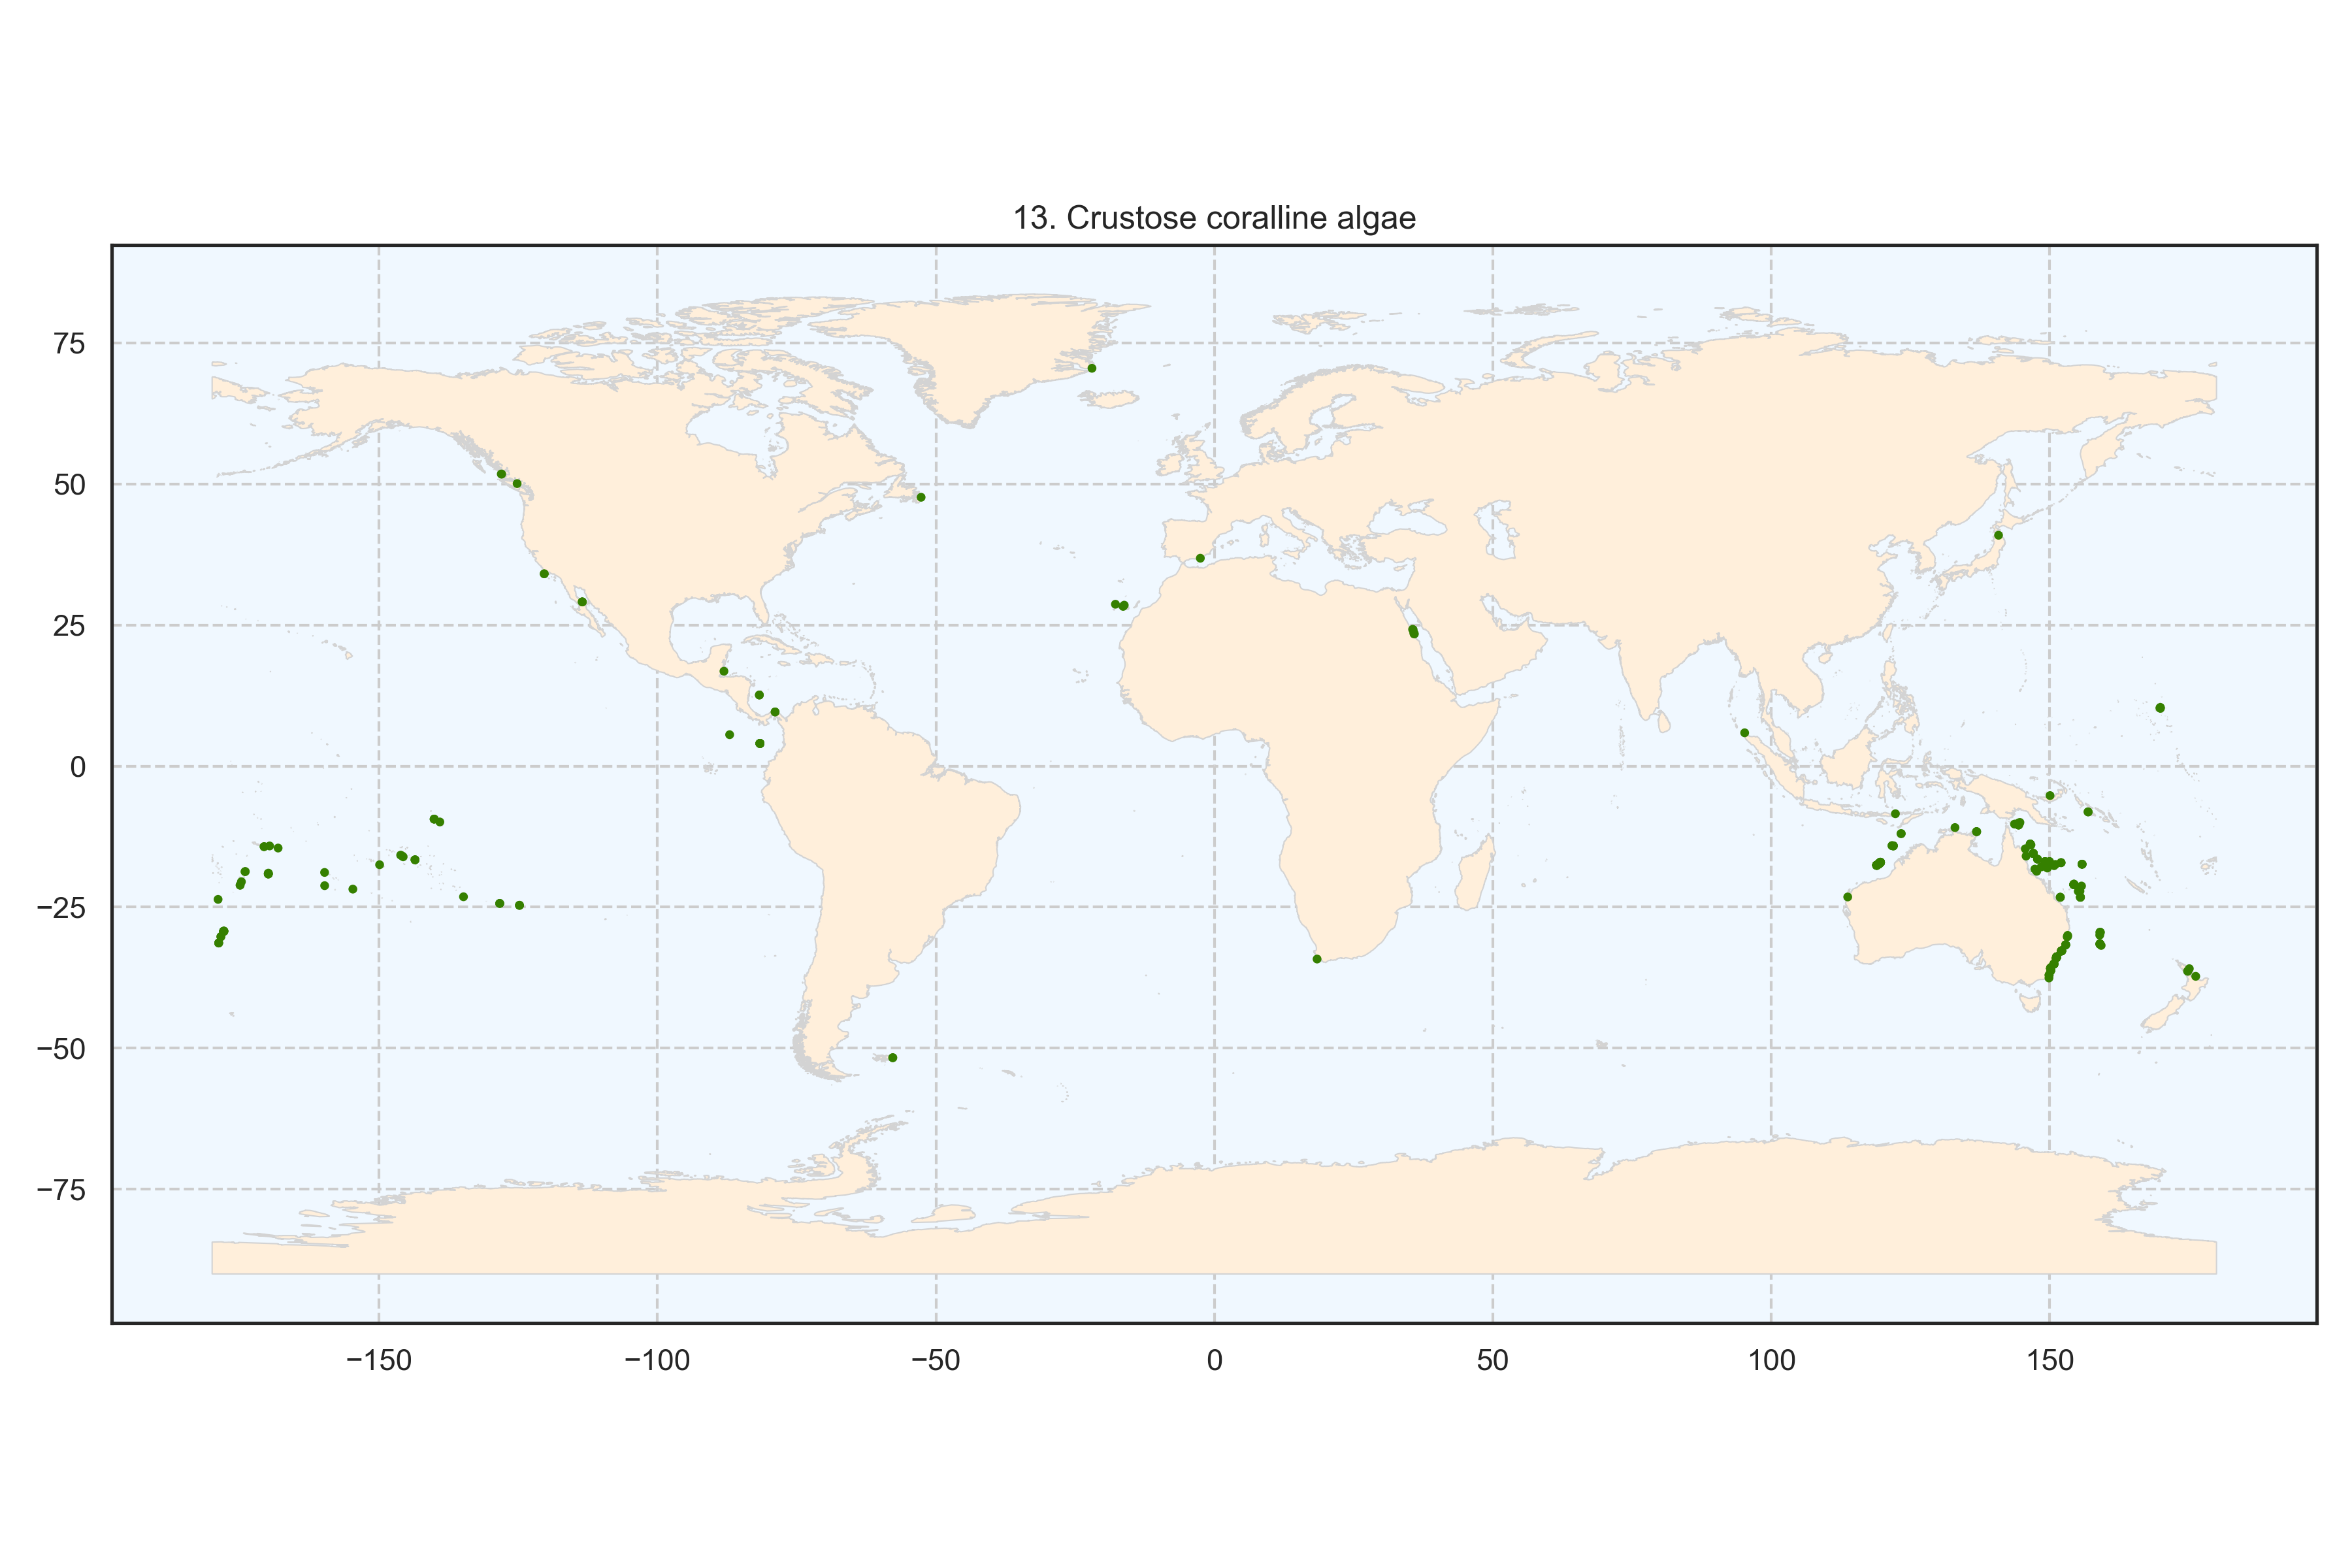
\includegraphics{03-Chapitre2/figures/supplementary/06-spatial-cluster_distribution_cluster_12.png}
\caption{Spatial distribution of the cluster \emph{crustose coralline
algae} at the global scale. Each point represents a
transect.}\label{fig:chap2figS15}
}
\end{figure}

\begin{figure}
\hypertarget{fig:chap2figS16}{%
\centering
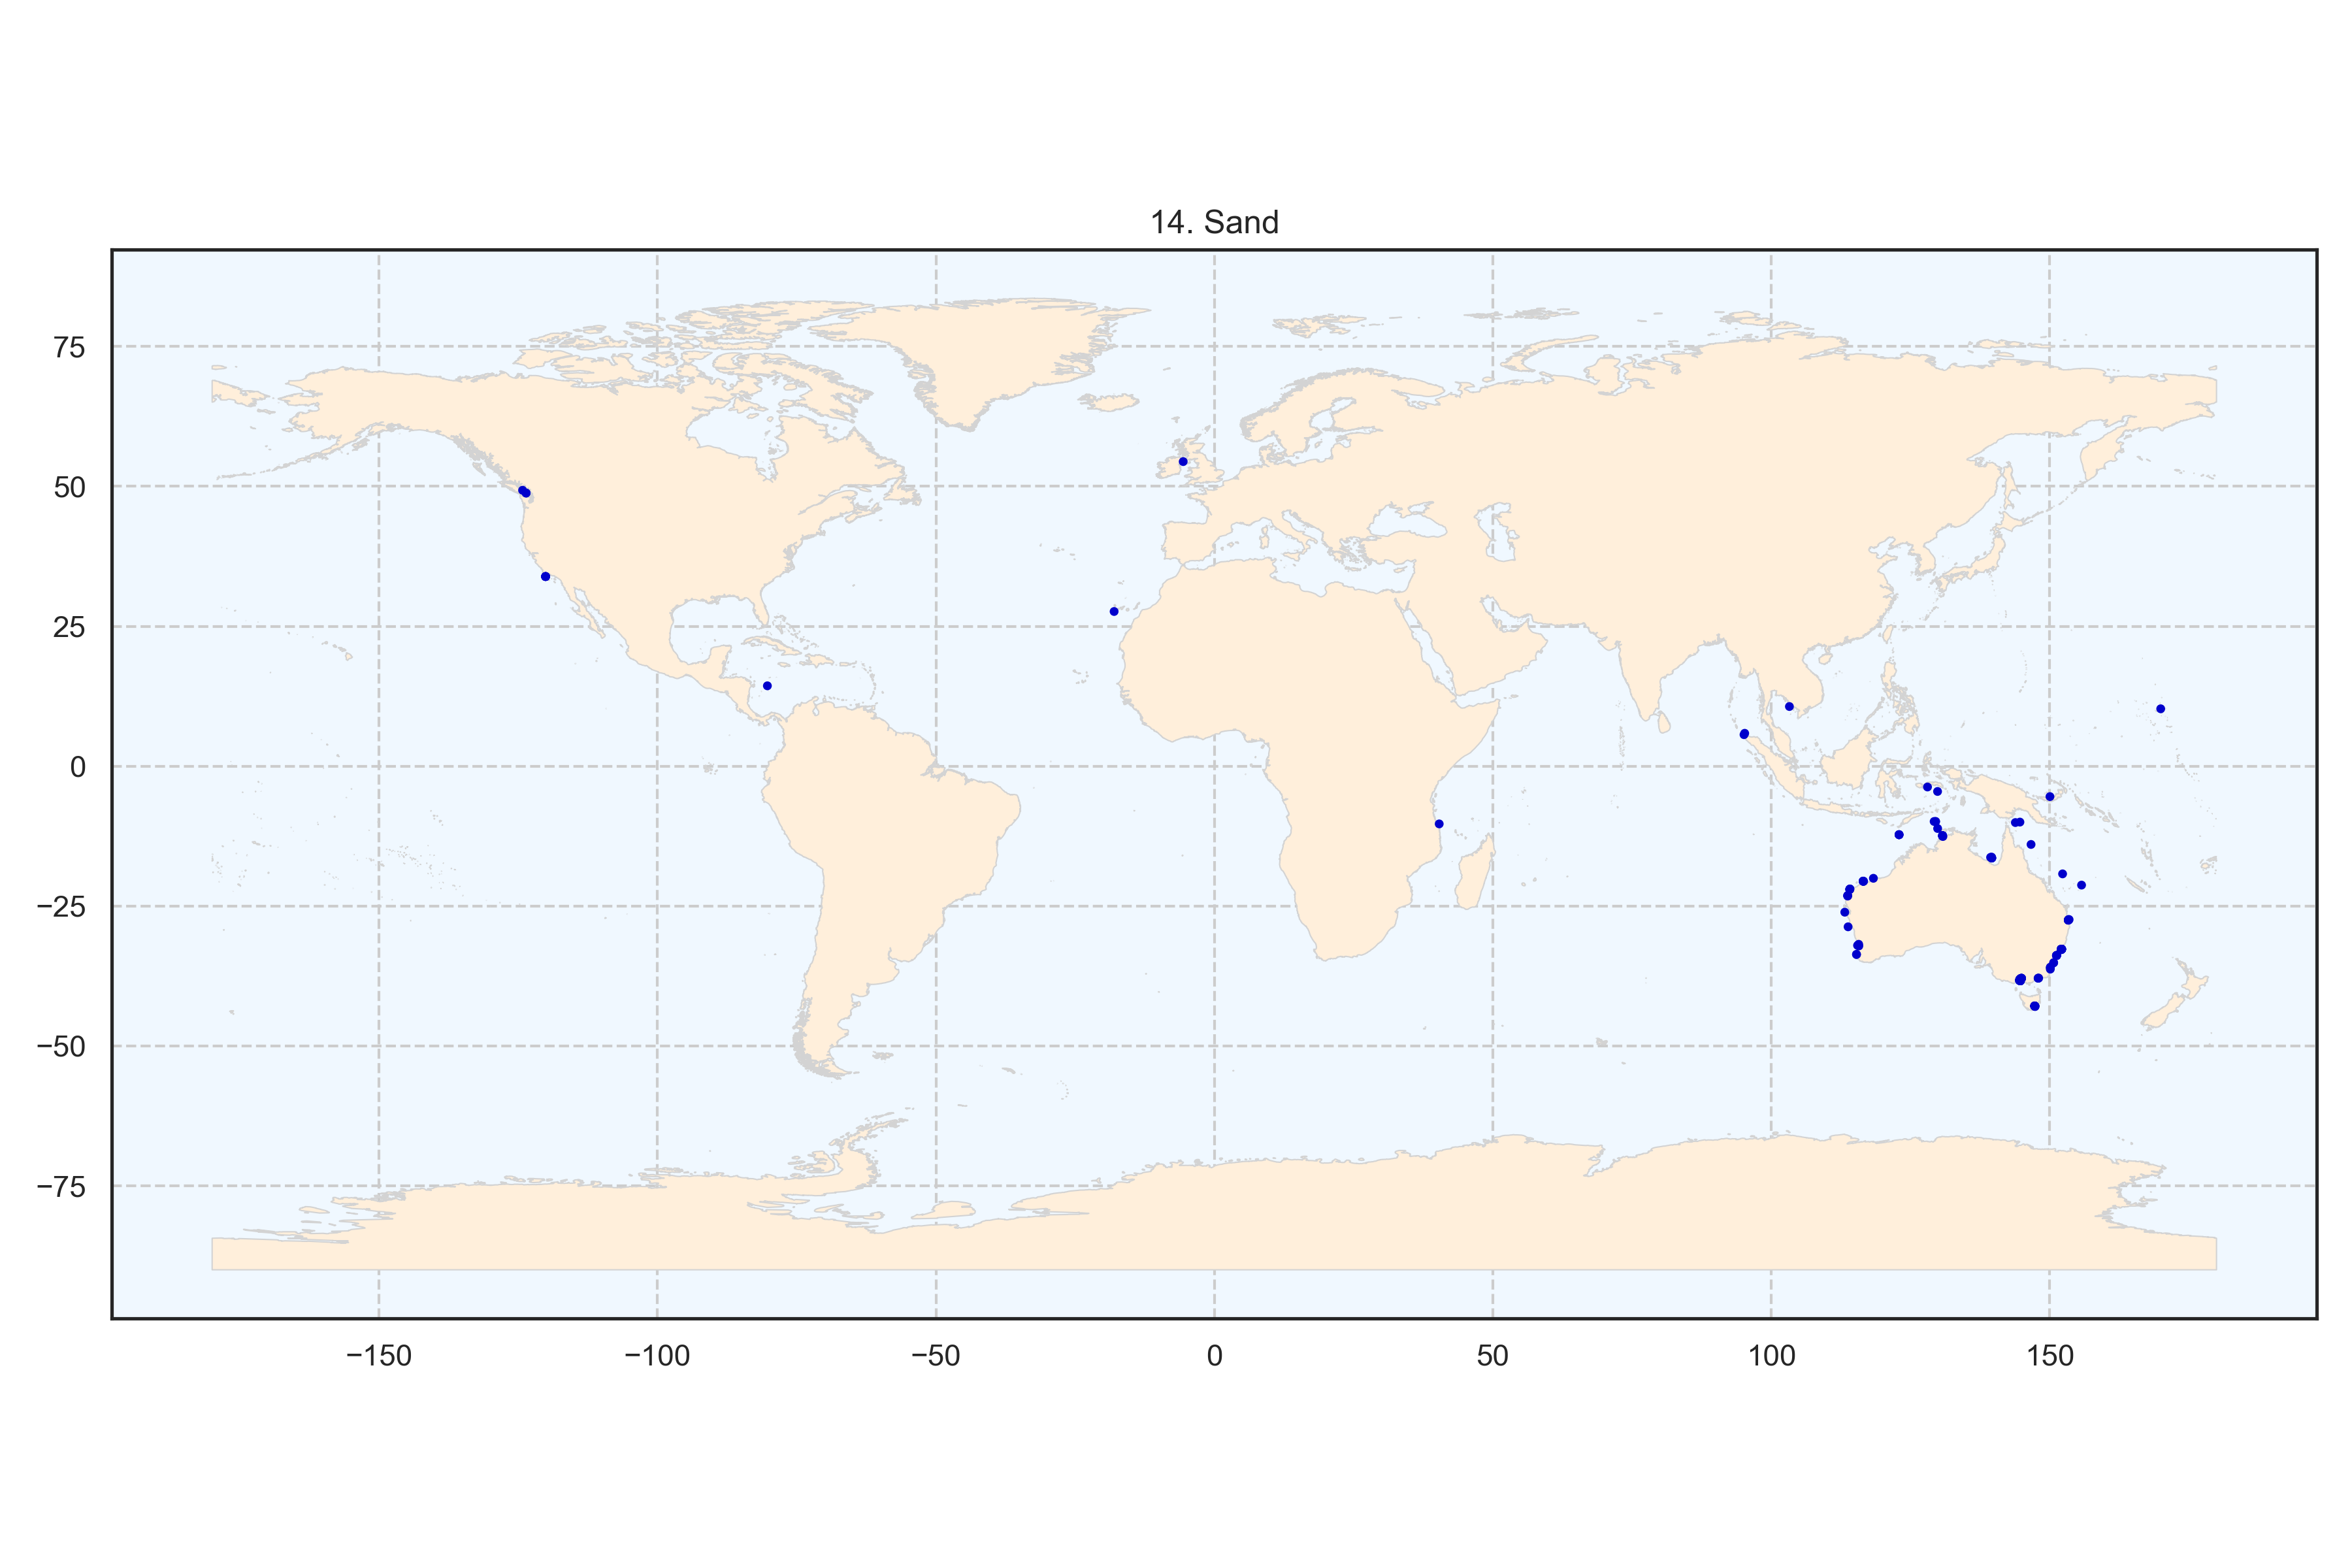
\includegraphics{03-Chapitre2/figures/supplementary/06-spatial-cluster_distribution_cluster_13.png}
\caption{Spatial distribution of the cluster \emph{sand} at the global
scale. Each point represents a transect.}\label{fig:chap2figS16}
}
\end{figure}

\begin{figure}
\hypertarget{fig:chap2figS17}{%
\centering
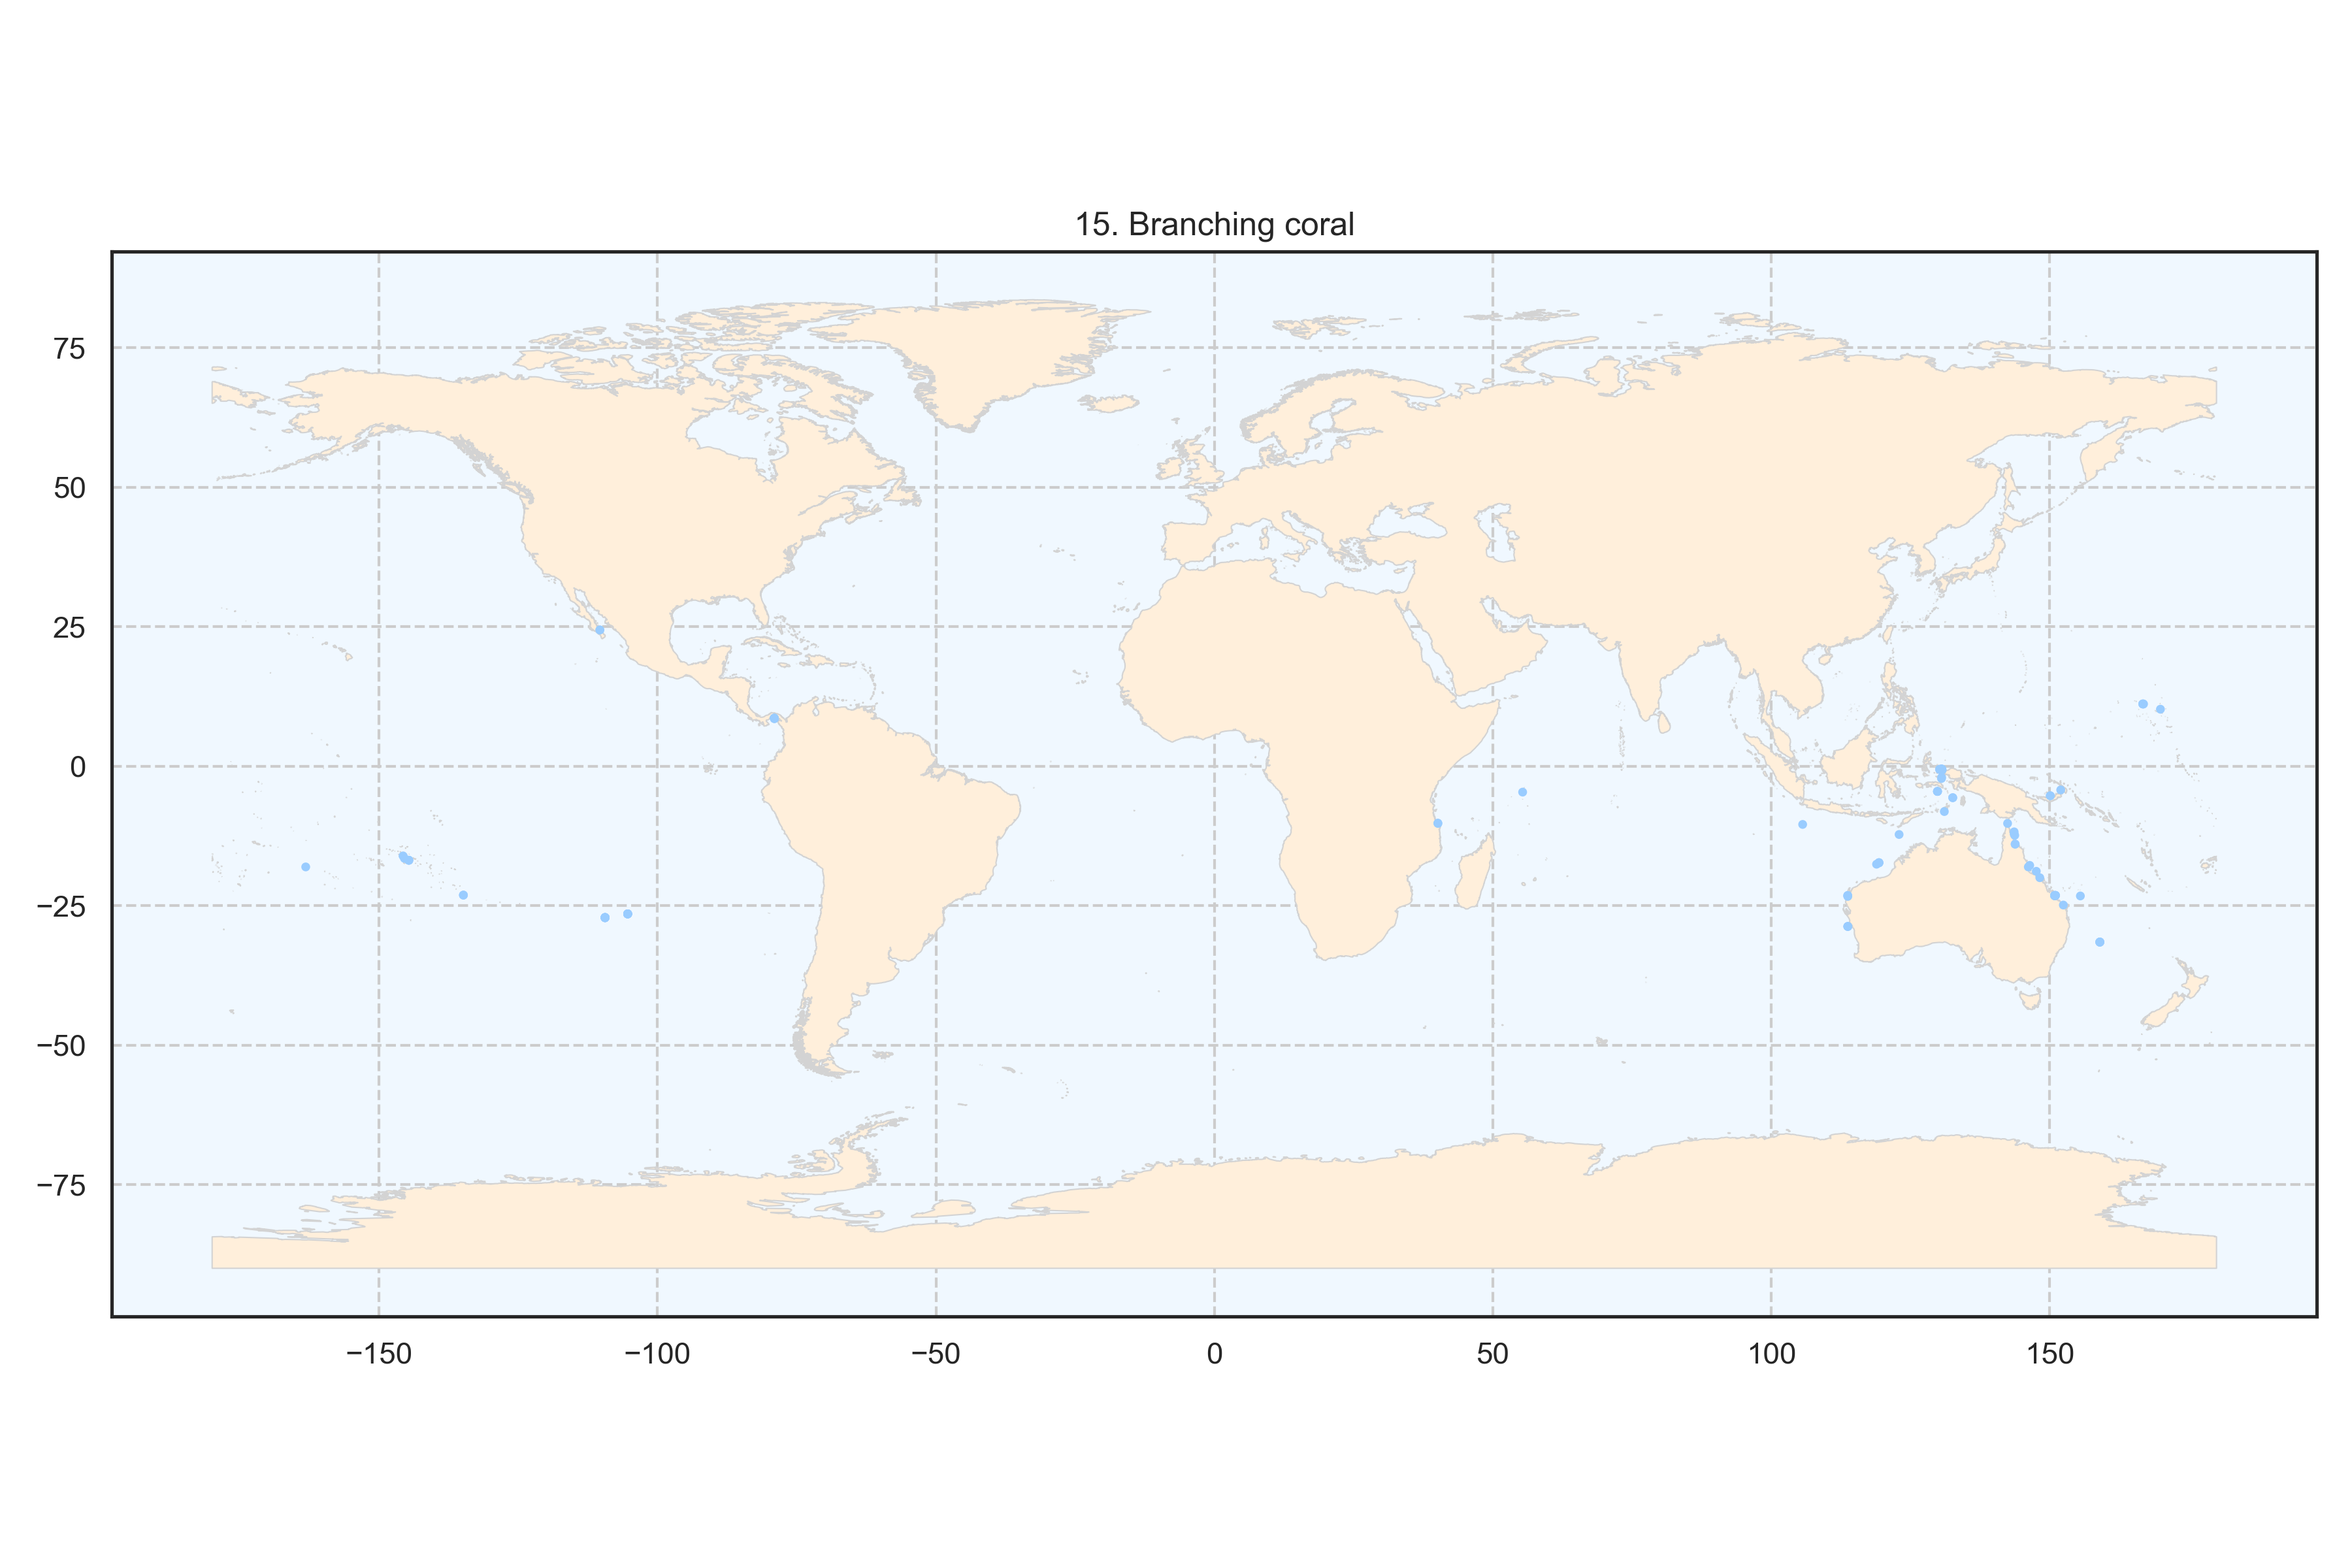
\includegraphics{03-Chapitre2/figures/supplementary/06-spatial-cluster_distribution_cluster_14.png}
\caption{Spatial distribution of the cluster \emph{branching coral} at
the global scale. Each point represents a
transect.}\label{fig:chap2figS17}
}
\end{figure}

\begin{figure}
\hypertarget{fig:chap2figS18}{%
\centering
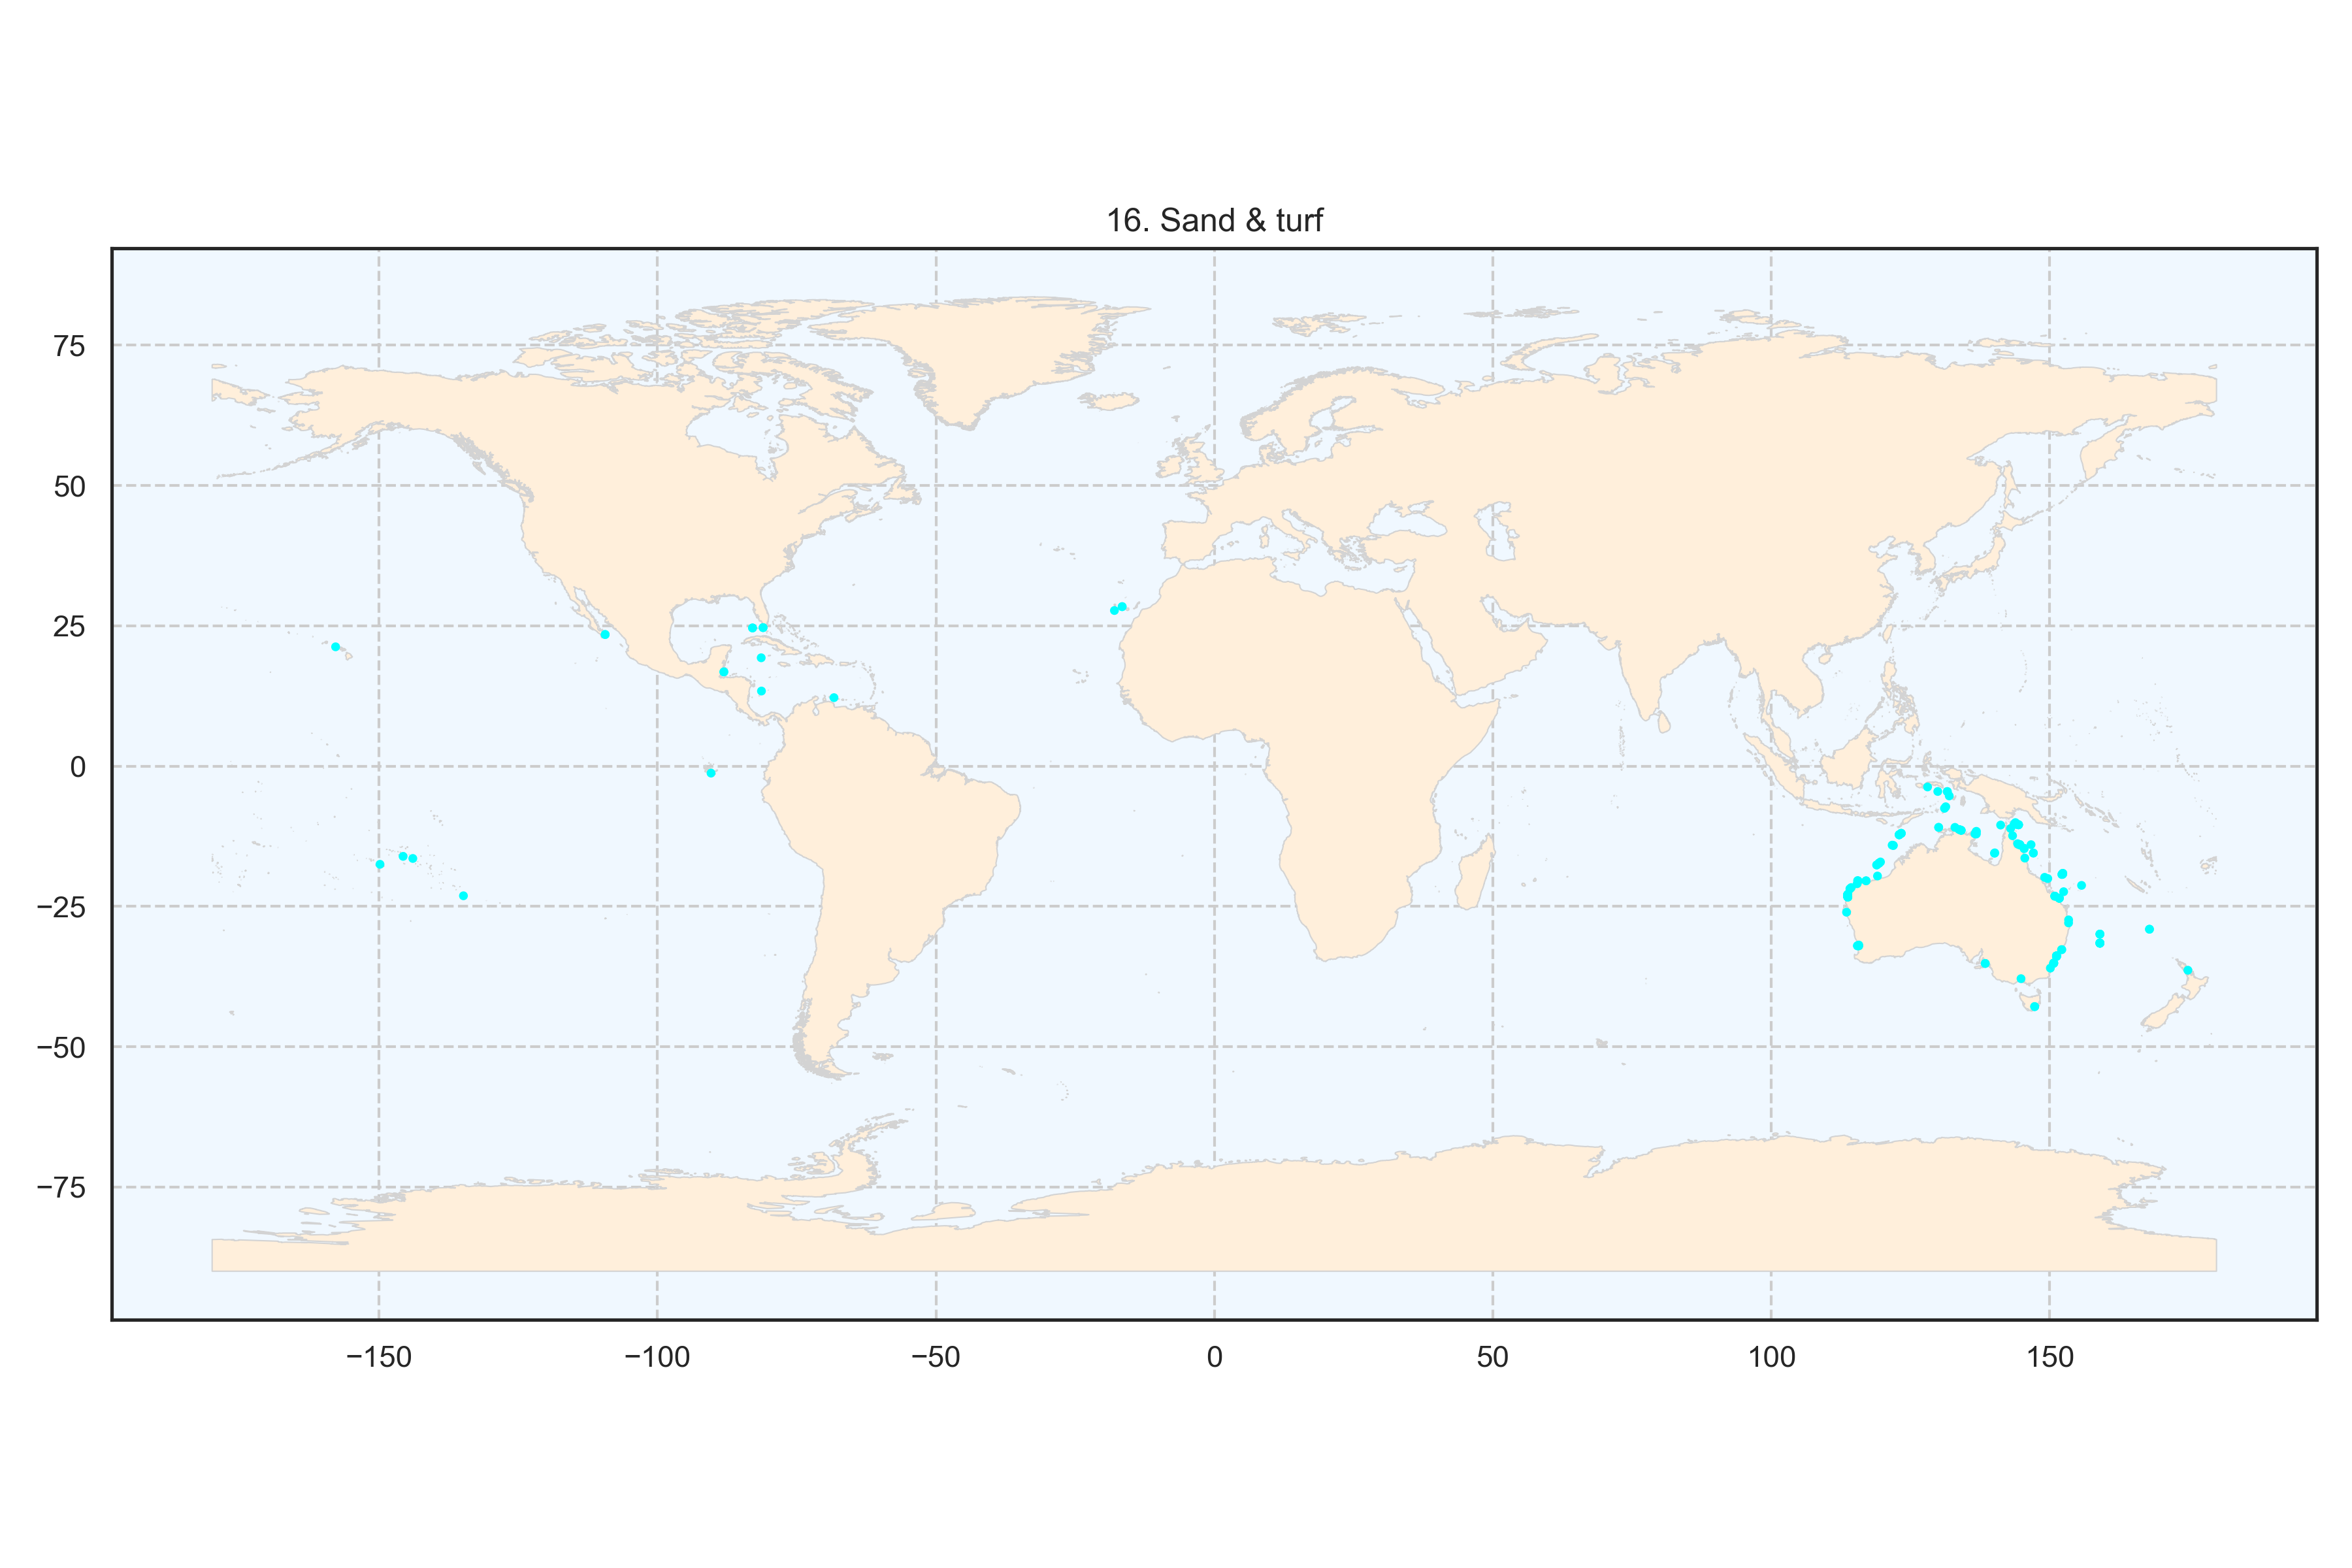
\includegraphics{03-Chapitre2/figures/supplementary/06-spatial-cluster_distribution_cluster_15.png}
\caption{Spatial distribution of the cluster \emph{sand and turf algae}
at the global scale. Each point represents a
transect.}\label{fig:chap2figS18}
}
\end{figure}

\begin{figure}
\hypertarget{fig:chap2figS19}{%
\centering
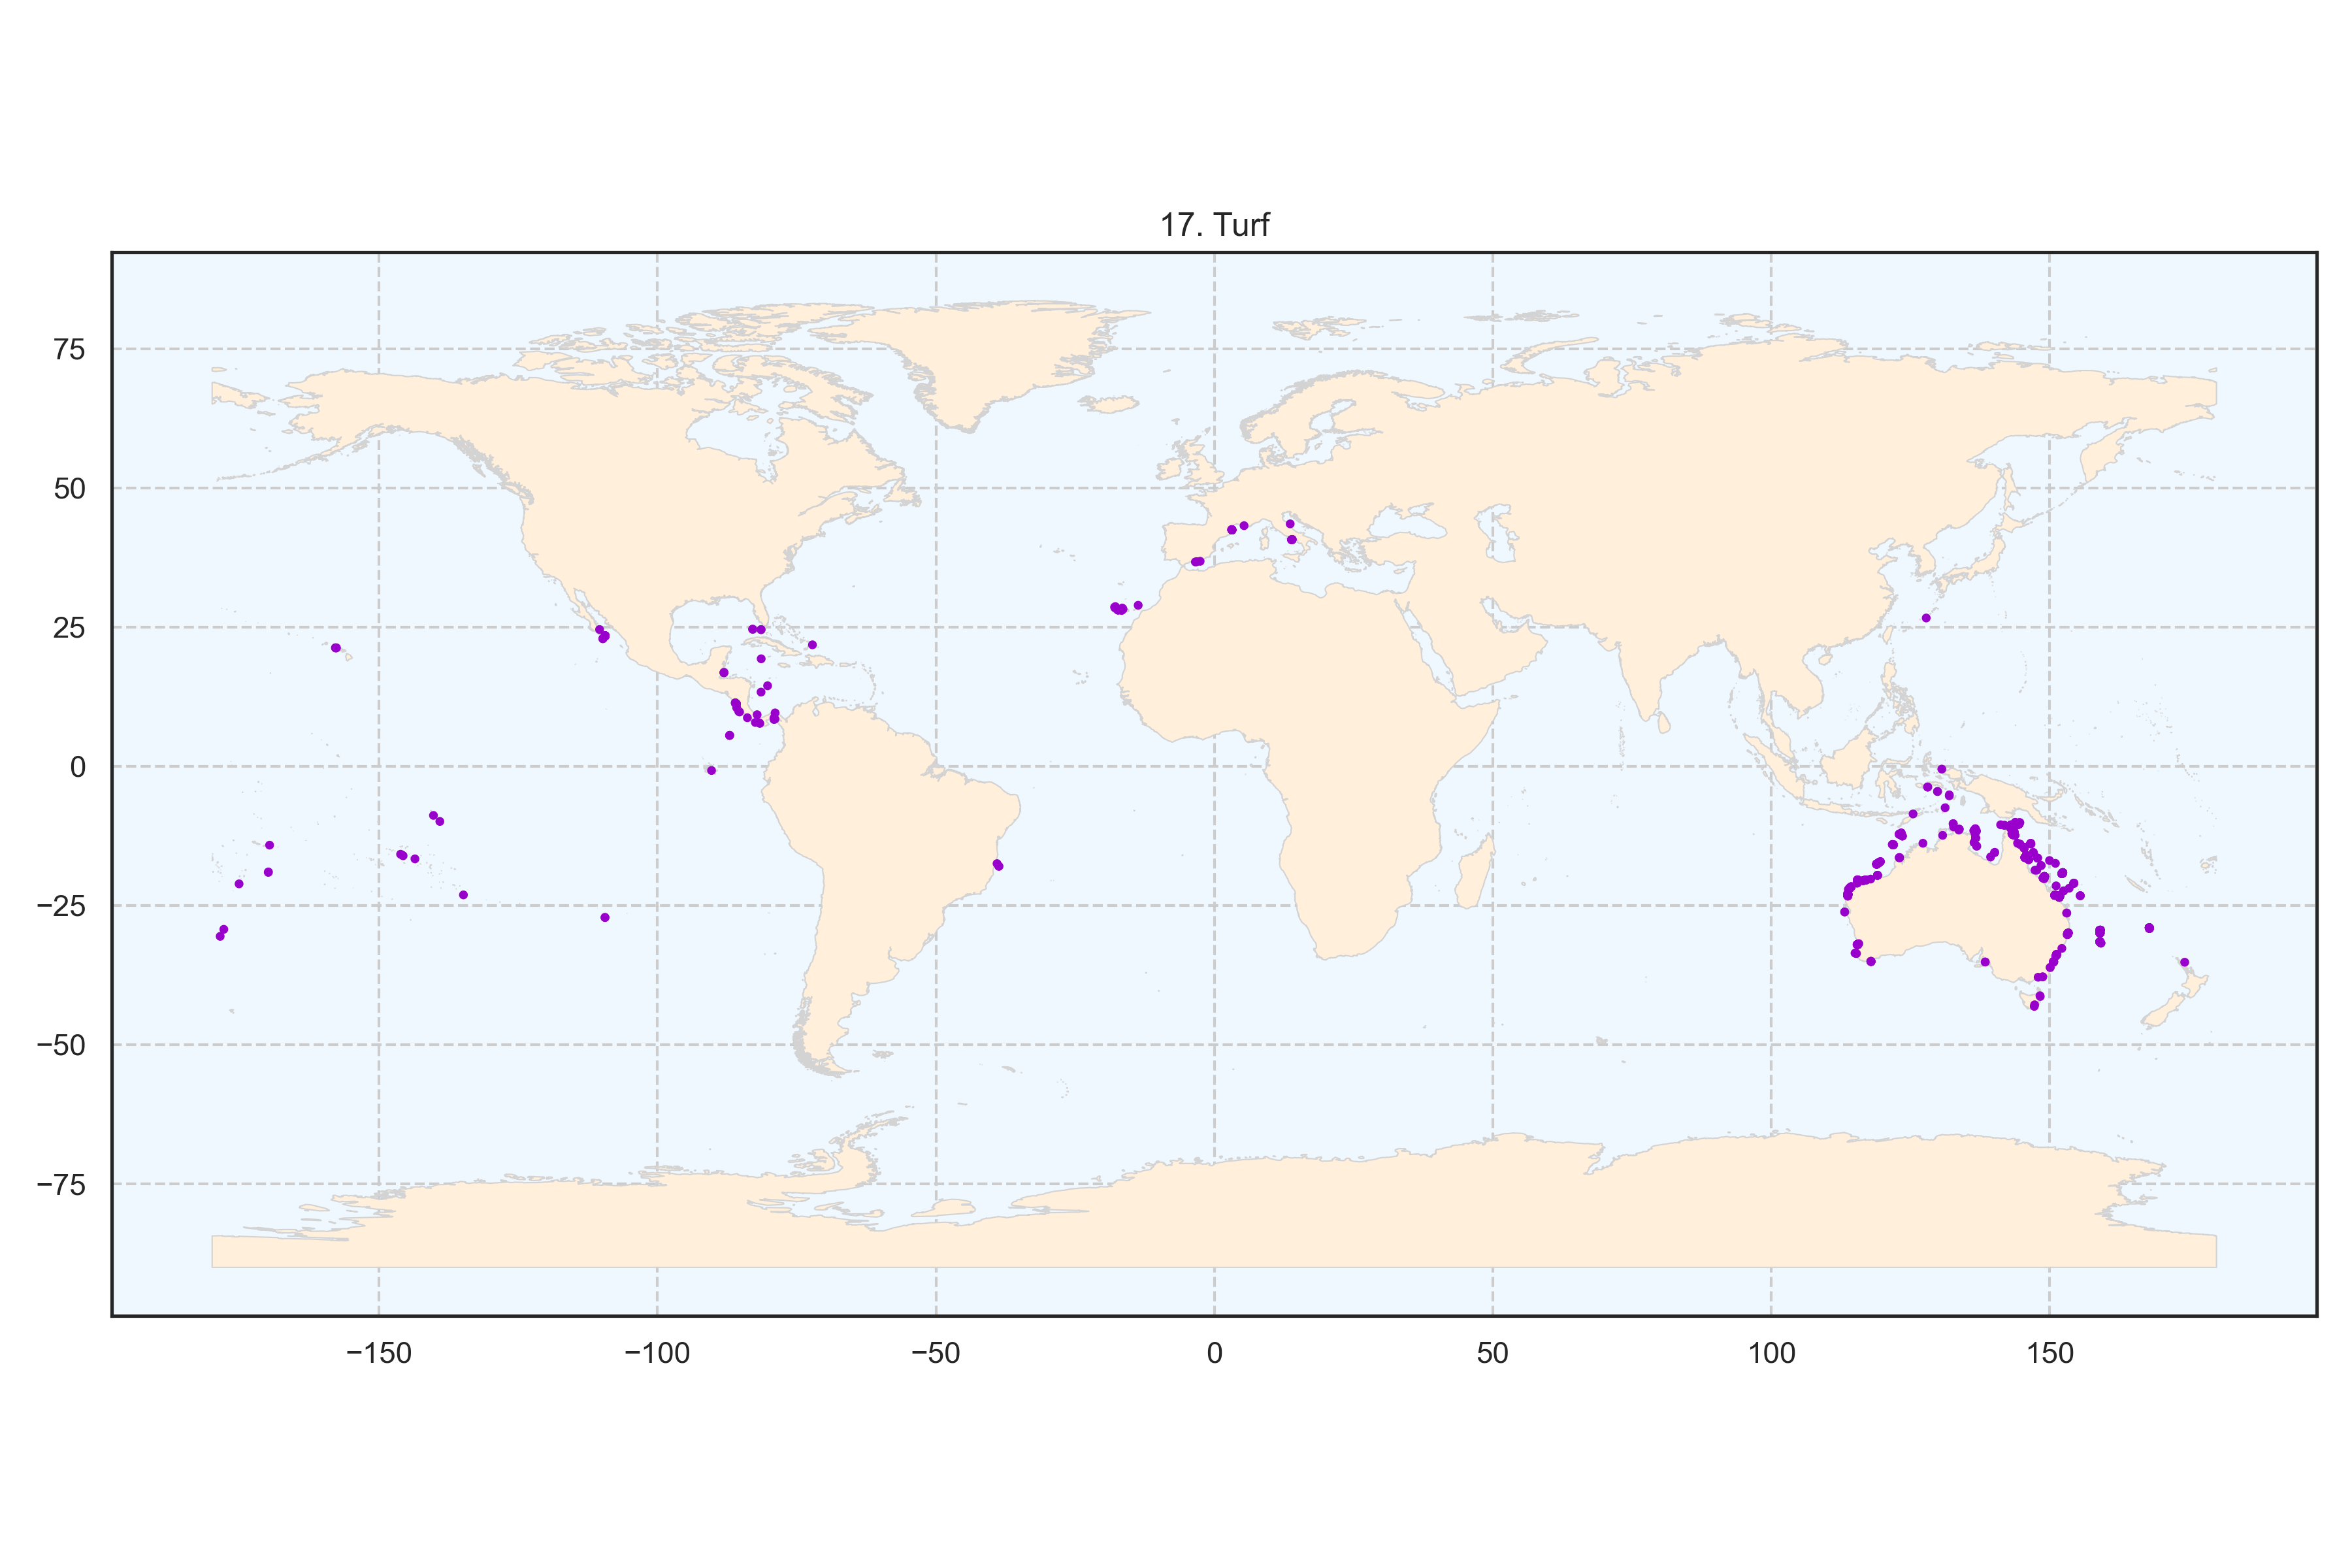
\includegraphics{03-Chapitre2/figures/supplementary/06-spatial-cluster_distribution_cluster_16.png}
\caption{Spatial distribution of the cluster \emph{turf algae} at the
global scale. Each point represents a transect.}\label{fig:chap2figS19}
}
\end{figure}

\clearpage

\hypertarget{appendixC-chapter2}{%
\section*{Appendix C - Interpretation of the uncovered
clusters}\label{appendixC-chapter2}}
\addcontentsline{toc}{section}{Appendix C - Interpretation of the
uncovered clusters}

\begin{figure}
\hypertarget{fig:chap2figS20}{%
\centering
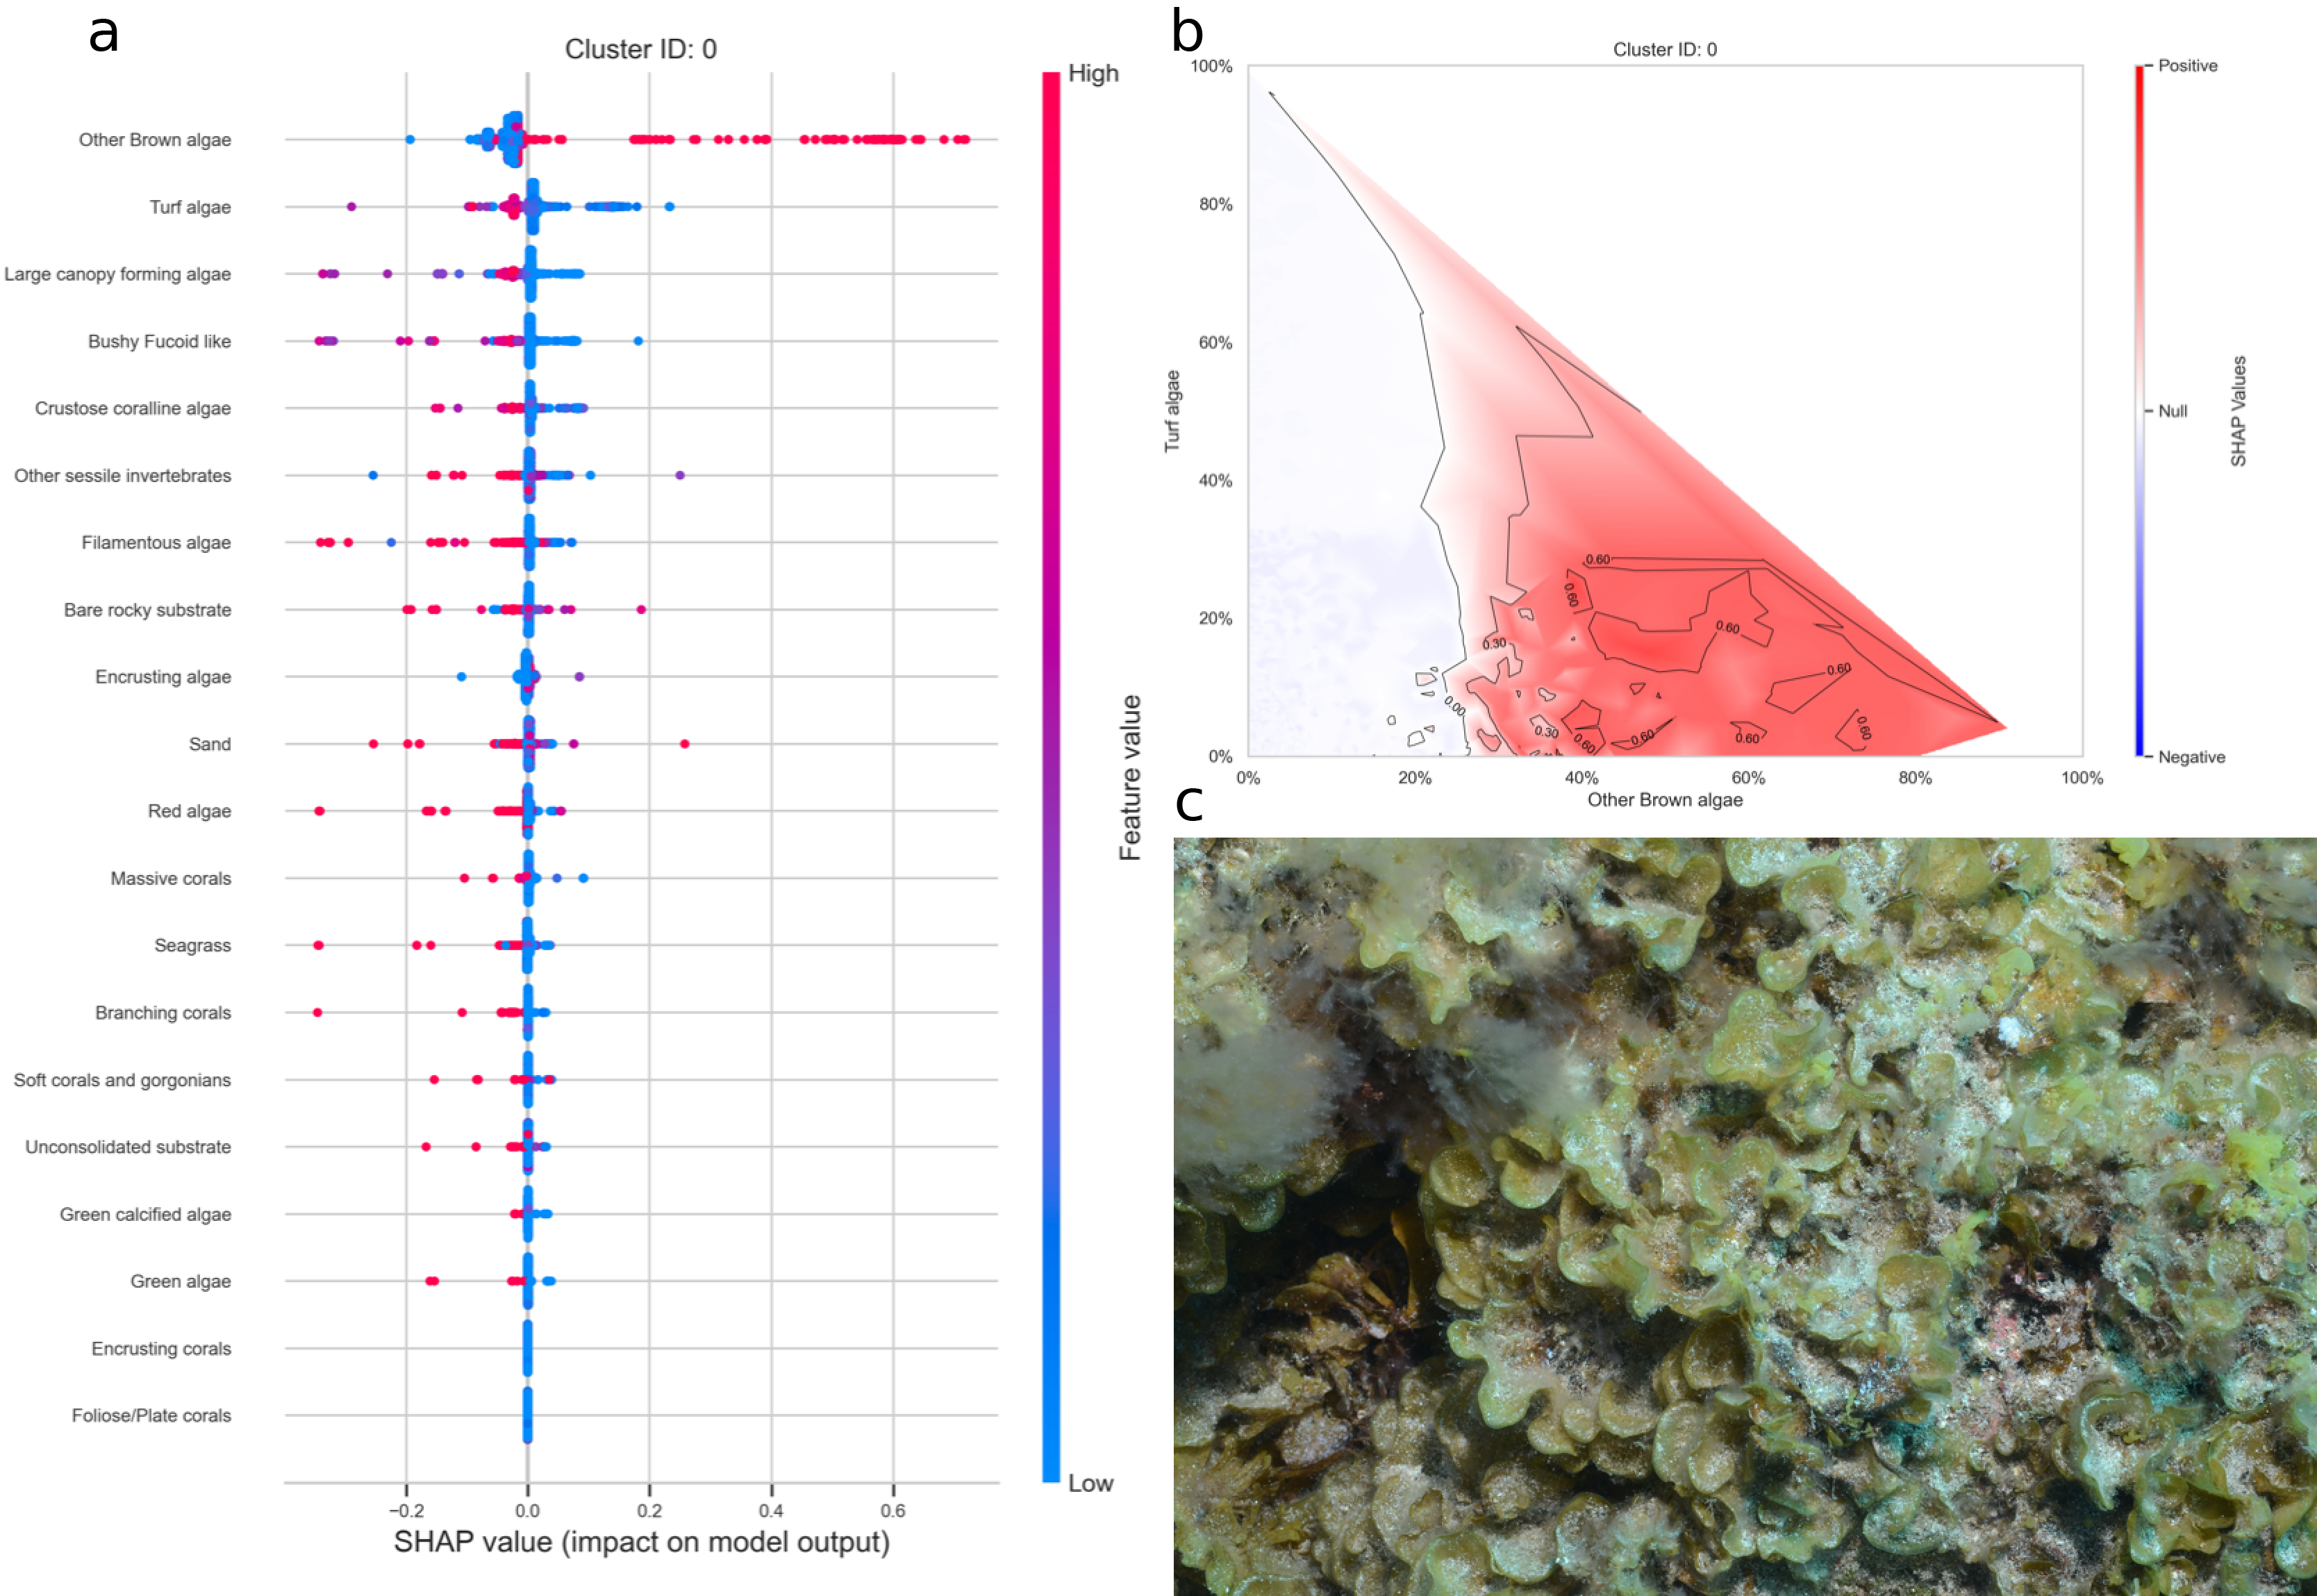
\includegraphics{03-Chapitre2/figures/supplementary/05-explanation_shap_pq_cluster_0.png}
\caption{a. \emph{SHAP} summary plot showing the impact of each habitat
substrate on the classification. The position of each habitat group on
the y-axis indicates its relative importance for the considered cluster.
The position of each point along the x-axis indicates if the observation
is associated with a lower or higher affinity with the cluster and the
colour of the point indicates if the value of the cover of this habitat
is rather high or low. b. Linear interpolation of the \emph{SHAP} values
for the two most influential variables for the cluster \emph{brown
algae}. c.~Example of photoquadrat for one transect of the cluster
\emph{brown algae} categorised by \emph{HDBSCAN} as
exemplary.}\label{fig:chap2figS20}
}
\end{figure}

\begin{figure}
\hypertarget{fig:chap2figS21}{%
\centering
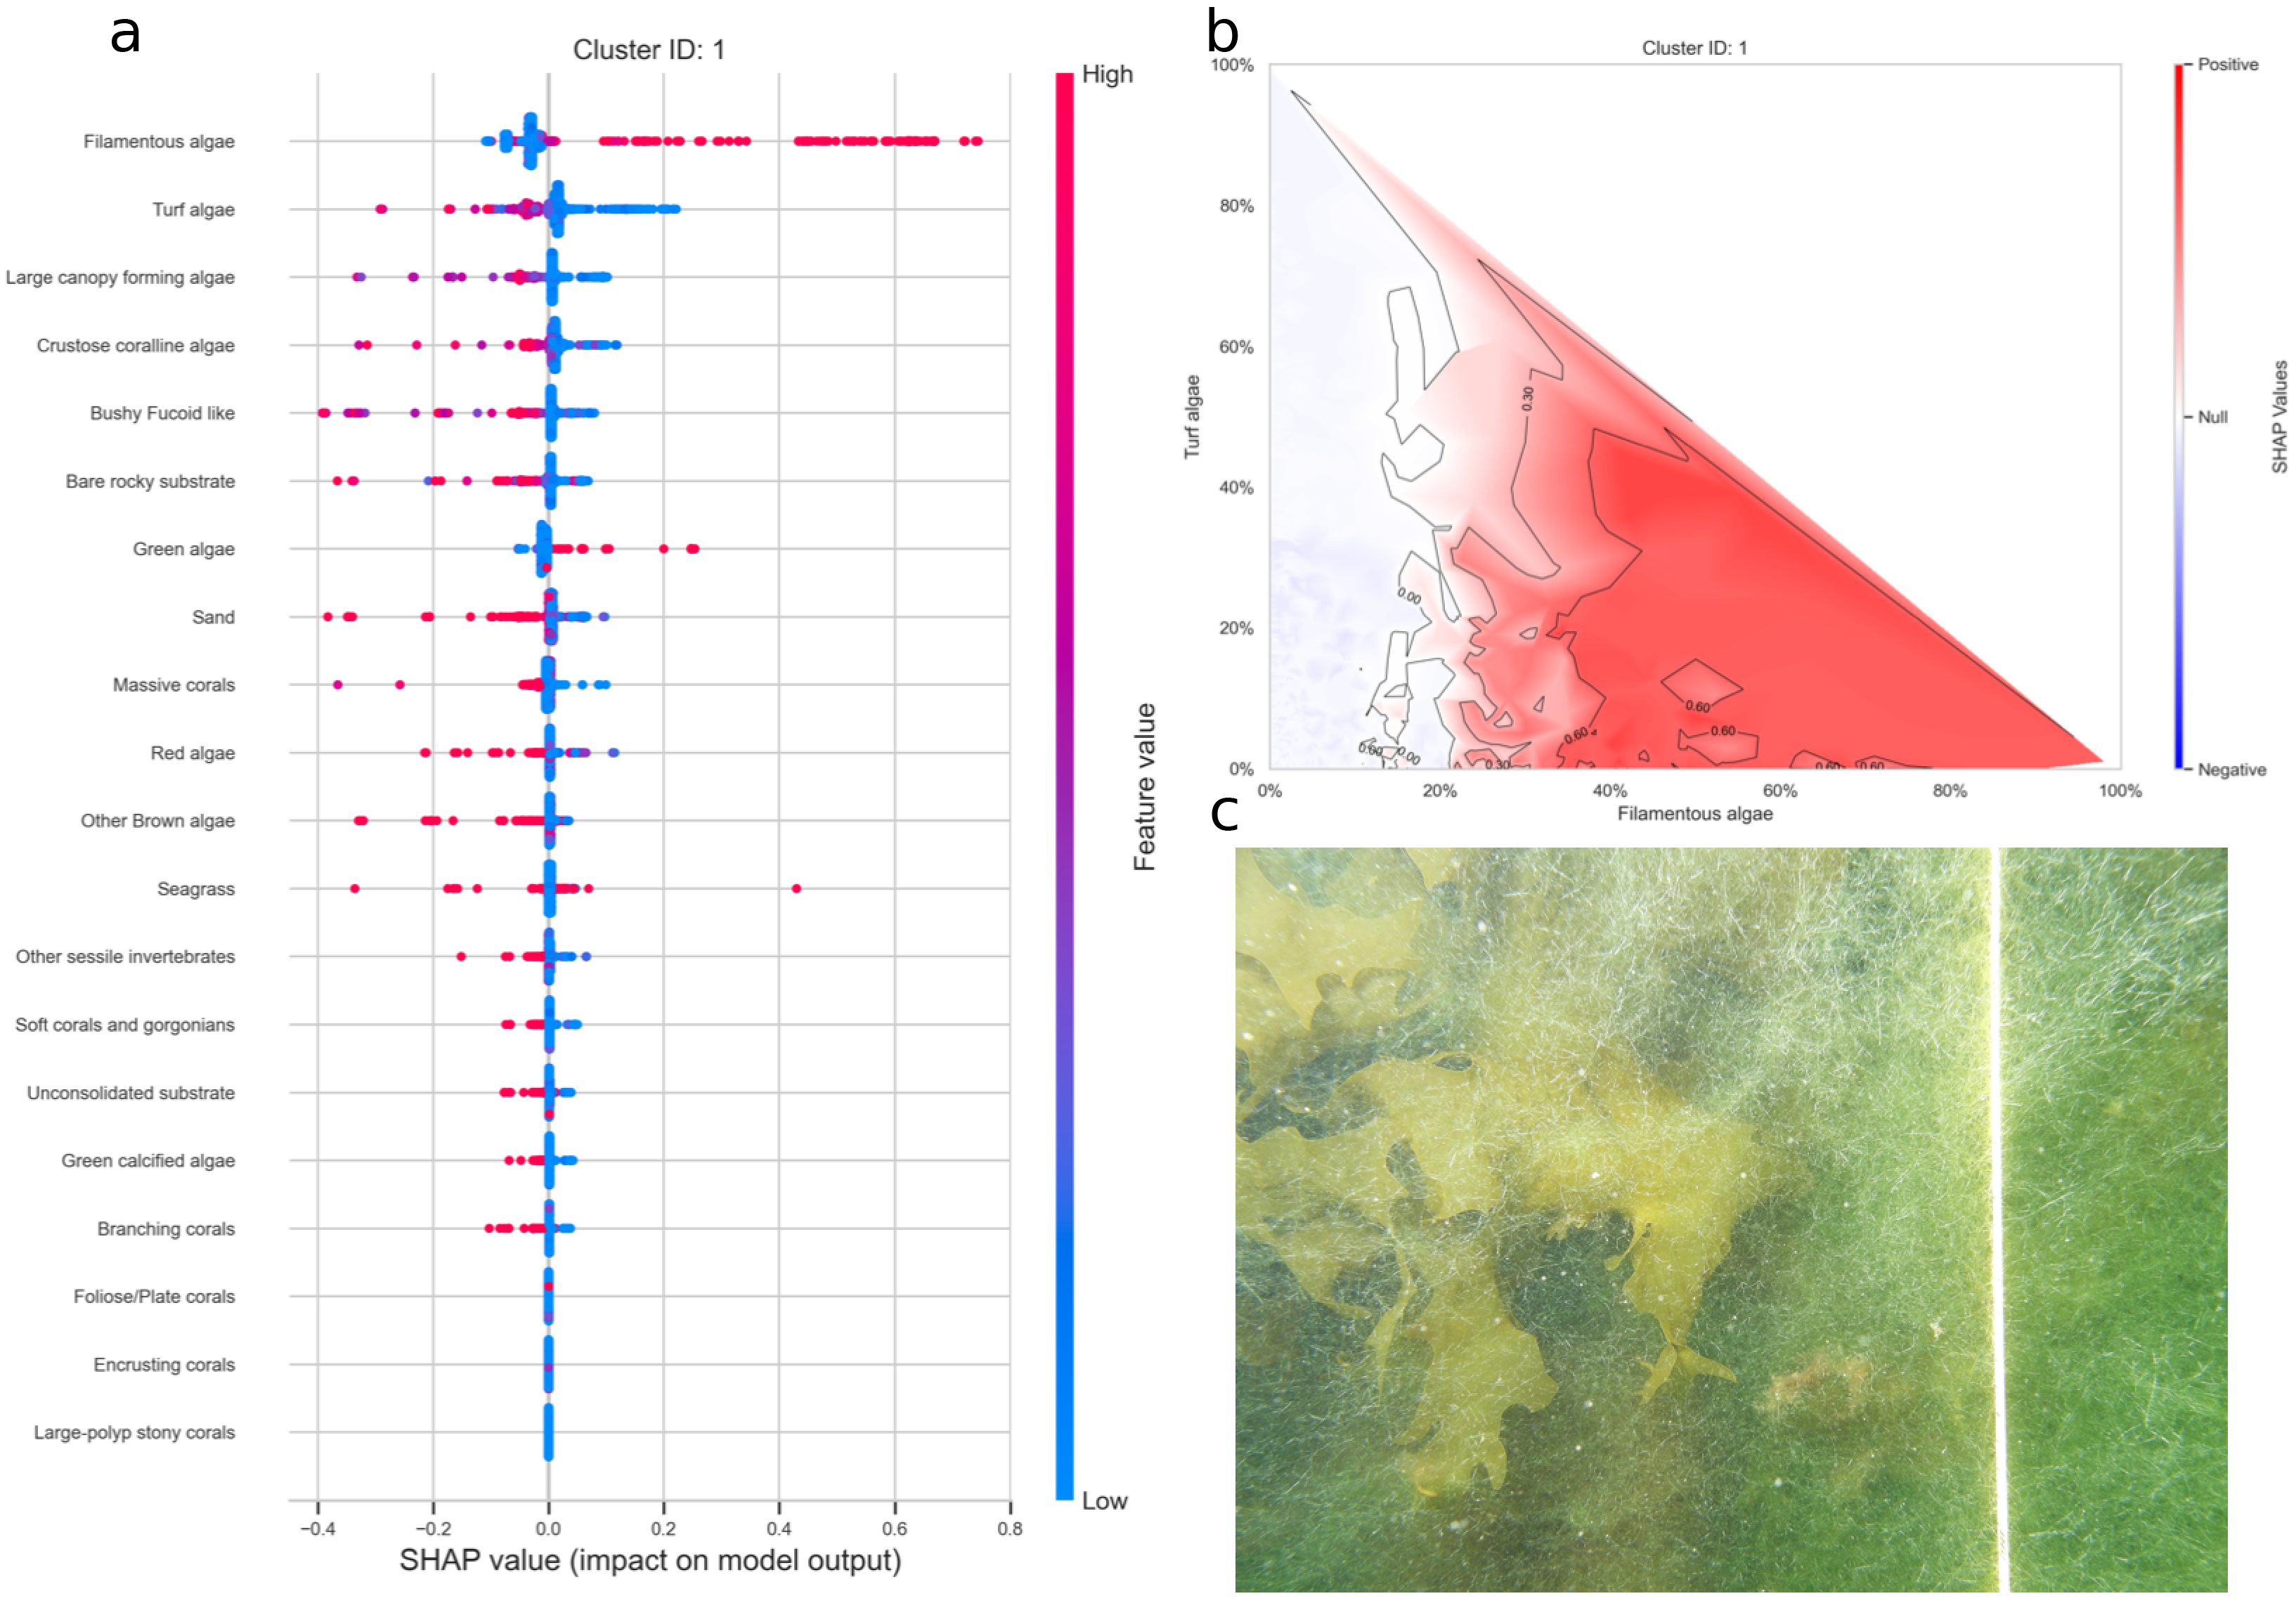
\includegraphics{03-Chapitre2/figures/supplementary/05-explanation_shap_pq_cluster_1.png}
\caption{a. \emph{SHAP} summary plot showing the impact of each habitat
substrate on the classification. The position of each habitat group on
the y-axis indicates its relative importance for the considered cluster.
The position of each point along the x-axis indicates if the observation
is associated with a lower or higher affinity with the cluster and the
colour of the point indicates if the value of the cover of this habitat
is rather high or low. b. Linear interpolation of the \emph{SHAP} values
for the two most influential variables for the cluster \emph{filamentous
algae}. c.~Example of photoquadrat for one transect of the cluster
\emph{filamentous algae} categorised by \emph{HDBSCAN} as
exemplary.}\label{fig:chap2figS21}
}
\end{figure}

\begin{figure}
\hypertarget{fig:chap2figS22}{%
\centering
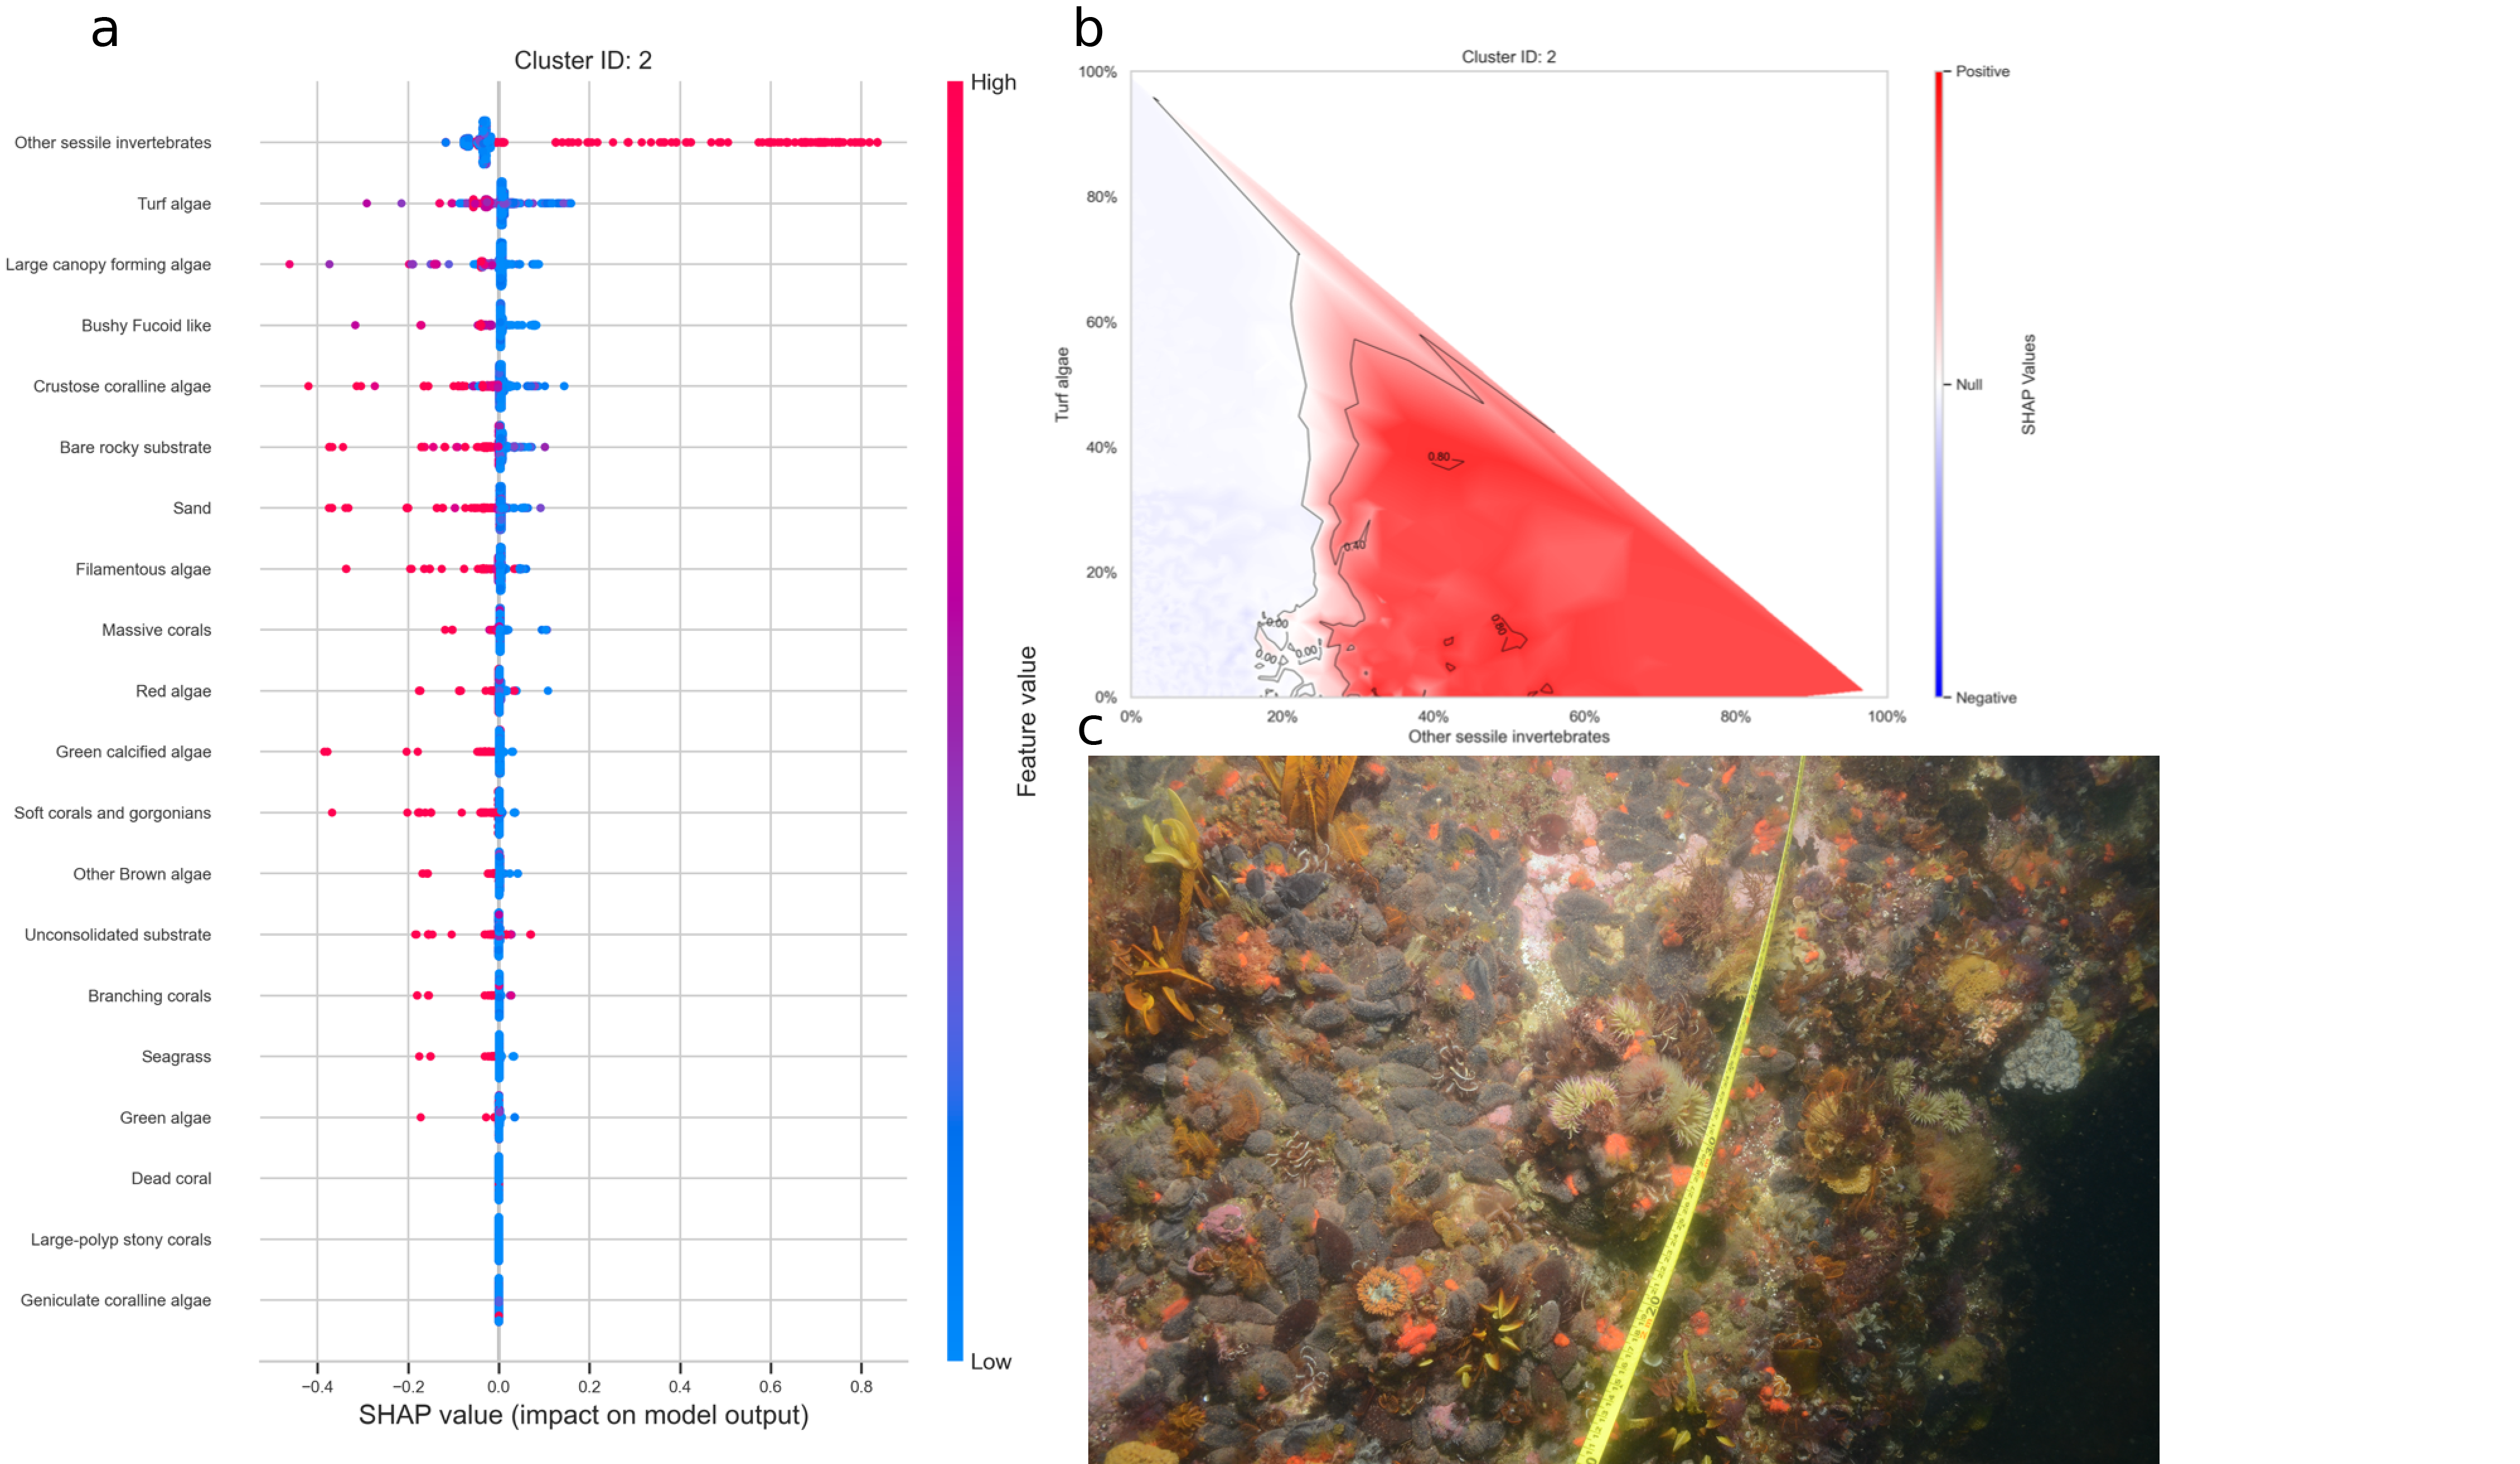
\includegraphics{03-Chapitre2/figures/supplementary/05-explanation_shap_pq_cluster_2.png}
\caption{a. \emph{SHAP} summary plot showing the impact of each habitat
substrate on the classification. The position of each habitat group on
the y-axis indicates its relative importance for the considered cluster.
The position of each point along the x-axis indicates if the observation
is associated with a lower or higher affinity with the cluster and the
colour of the point indicates if the value of the cover of this habitat
is rather high or low. b. Linear interpolation of the \emph{SHAP} values
for the two most influential variables for the cluster \emph{sessile
invertebrates}. c.~Example of photoquadrat for one transect of the
cluster \emph{sessile invertebrates} categorised by \emph{HDBSCAN} as
exemplary.}\label{fig:chap2figS22}
}
\end{figure}

\begin{figure}
\hypertarget{fig:chap2figS23}{%
\centering
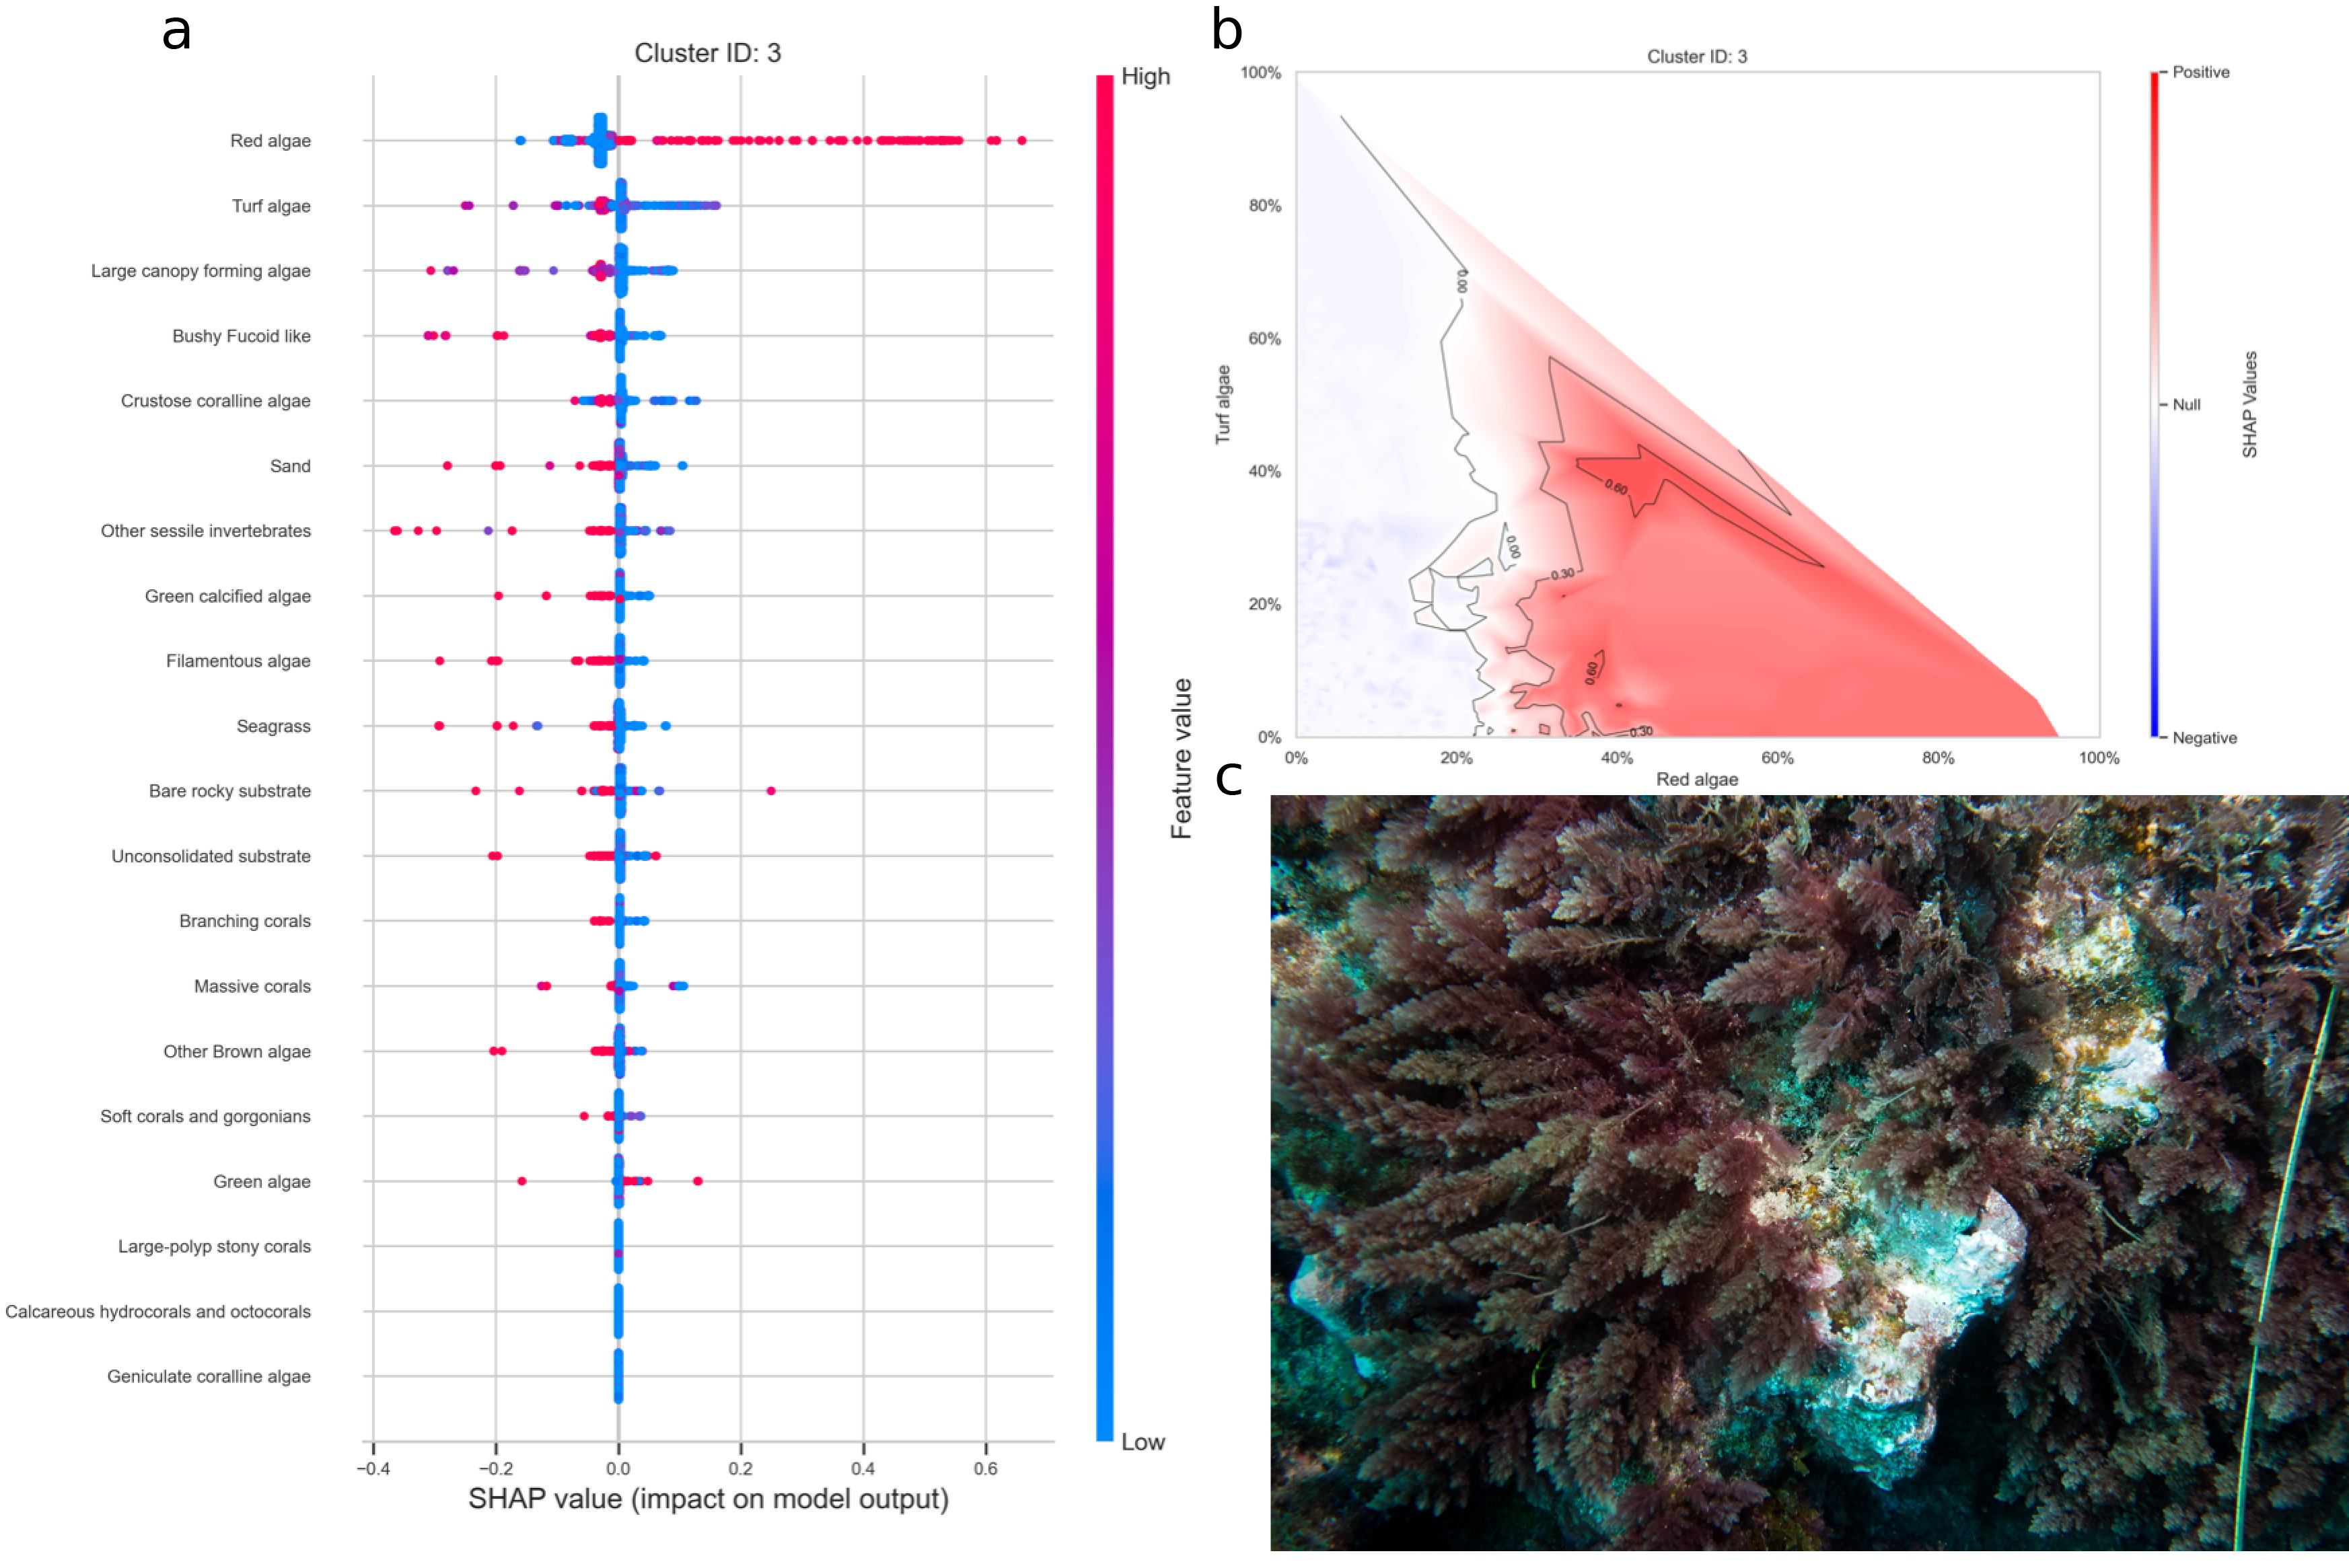
\includegraphics{03-Chapitre2/figures/supplementary/05-explanation_shap_pq_cluster_3.png}
\caption{a. \emph{SHAP} summary plot showing the impact of each habitat
substrate on the classification. The position of each habitat group on
the y-axis indicates its relative importance for the considered cluster.
The position of each point along the x-axis indicates if the observation
is associated with a lower or higher affinity with the cluster and the
colour of the point indicates if the value of the cover of this habitat
is rather high or low. b. Linear interpolation of the \emph{SHAP} values
for the two most influential variables for the cluster \emph{red algae}.
c.~Example of photoquadrat for one transect of the cluster \emph{red
algae} categorised by \emph{HDBSCAN} as
exemplary.}\label{fig:chap2figS23}
}
\end{figure}

\begin{figure}
\hypertarget{fig:chap2figS24}{%
\centering
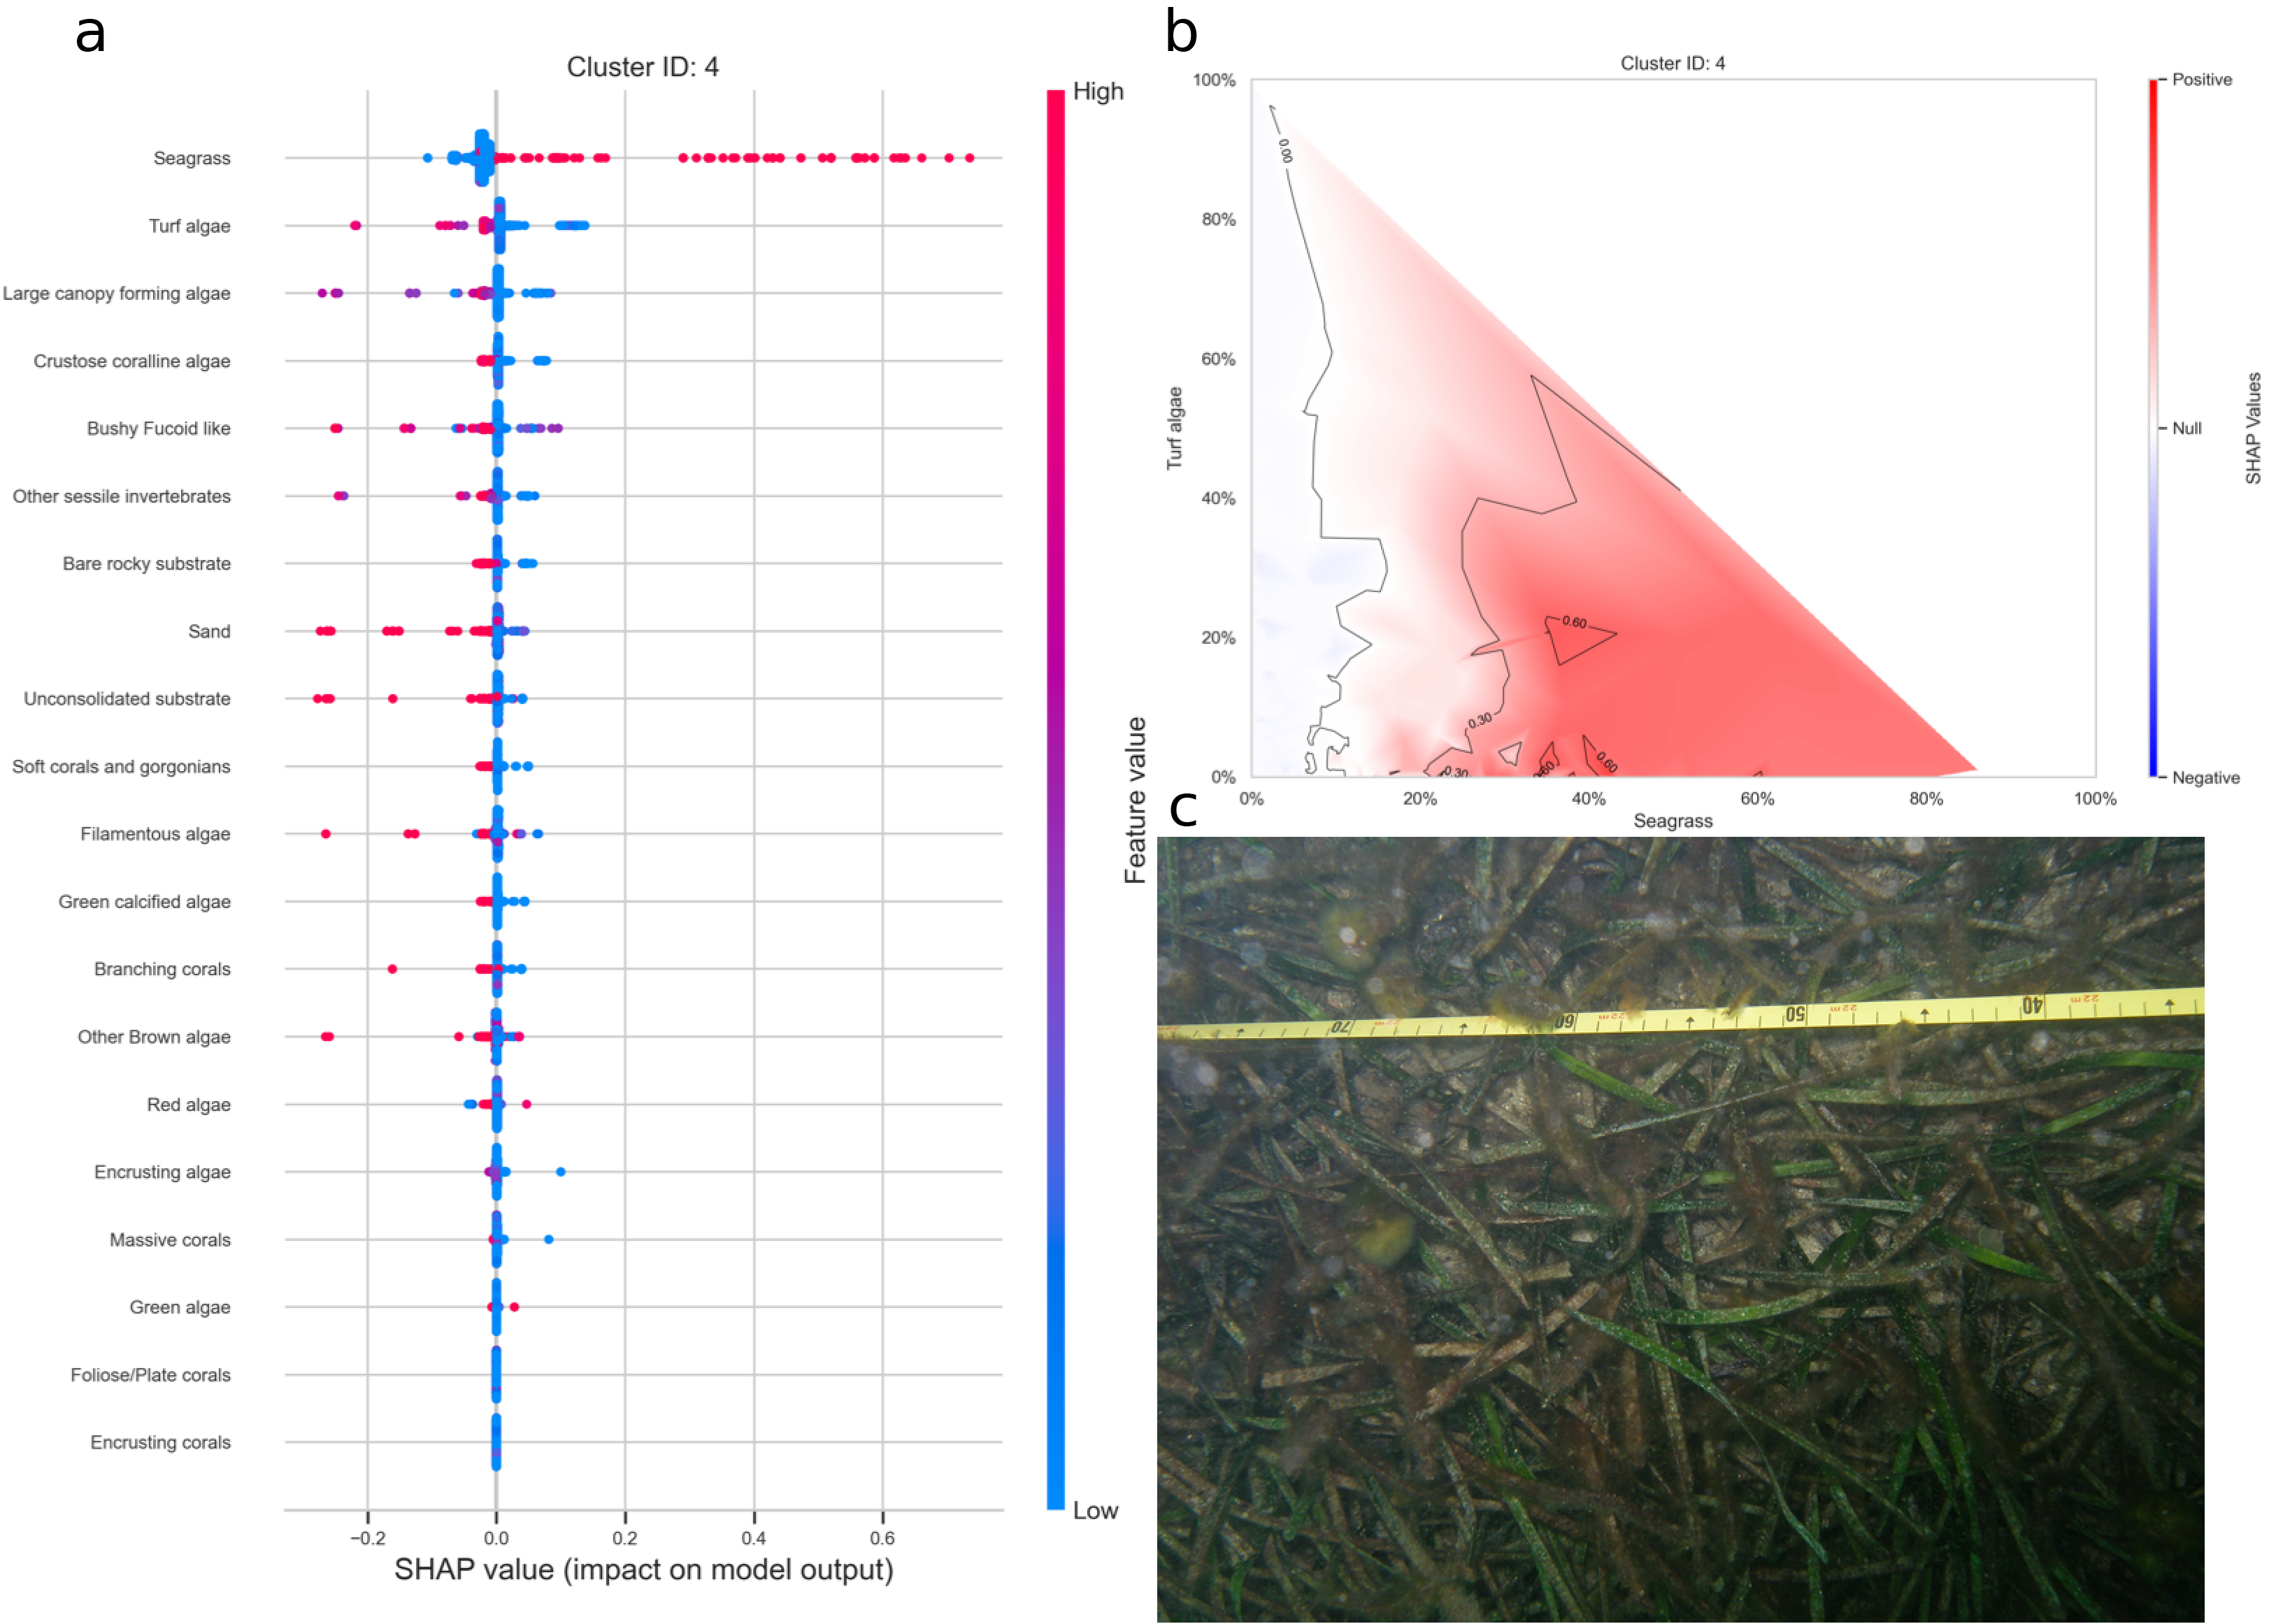
\includegraphics{03-Chapitre2/figures/supplementary/05-explanation_shap_pq_cluster_4.png}
\caption{a. \emph{SHAP} summary plot showing the impact of each habitat
substrate on the classification. The position of each habitat group on
the y-axis indicates its relative importance for the considered cluster.
The position of each point along the x-axis indicates if the observation
is associated with a lower or higher affinity with the cluster and the
colour of the point indicates if the value of the cover of this habitat
is rather high or low. b. Linear interpolation of the \emph{SHAP} values
for the two most influential variables for the cluster \emph{seagrass}.
c.~Example of photoquadrat for one transect of the cluster
\emph{seagrass} categorised by \emph{HDBSCAN} as
exemplary.}\label{fig:chap2figS24}
}
\end{figure}

\begin{figure}
\hypertarget{fig:chap2figS25}{%
\centering
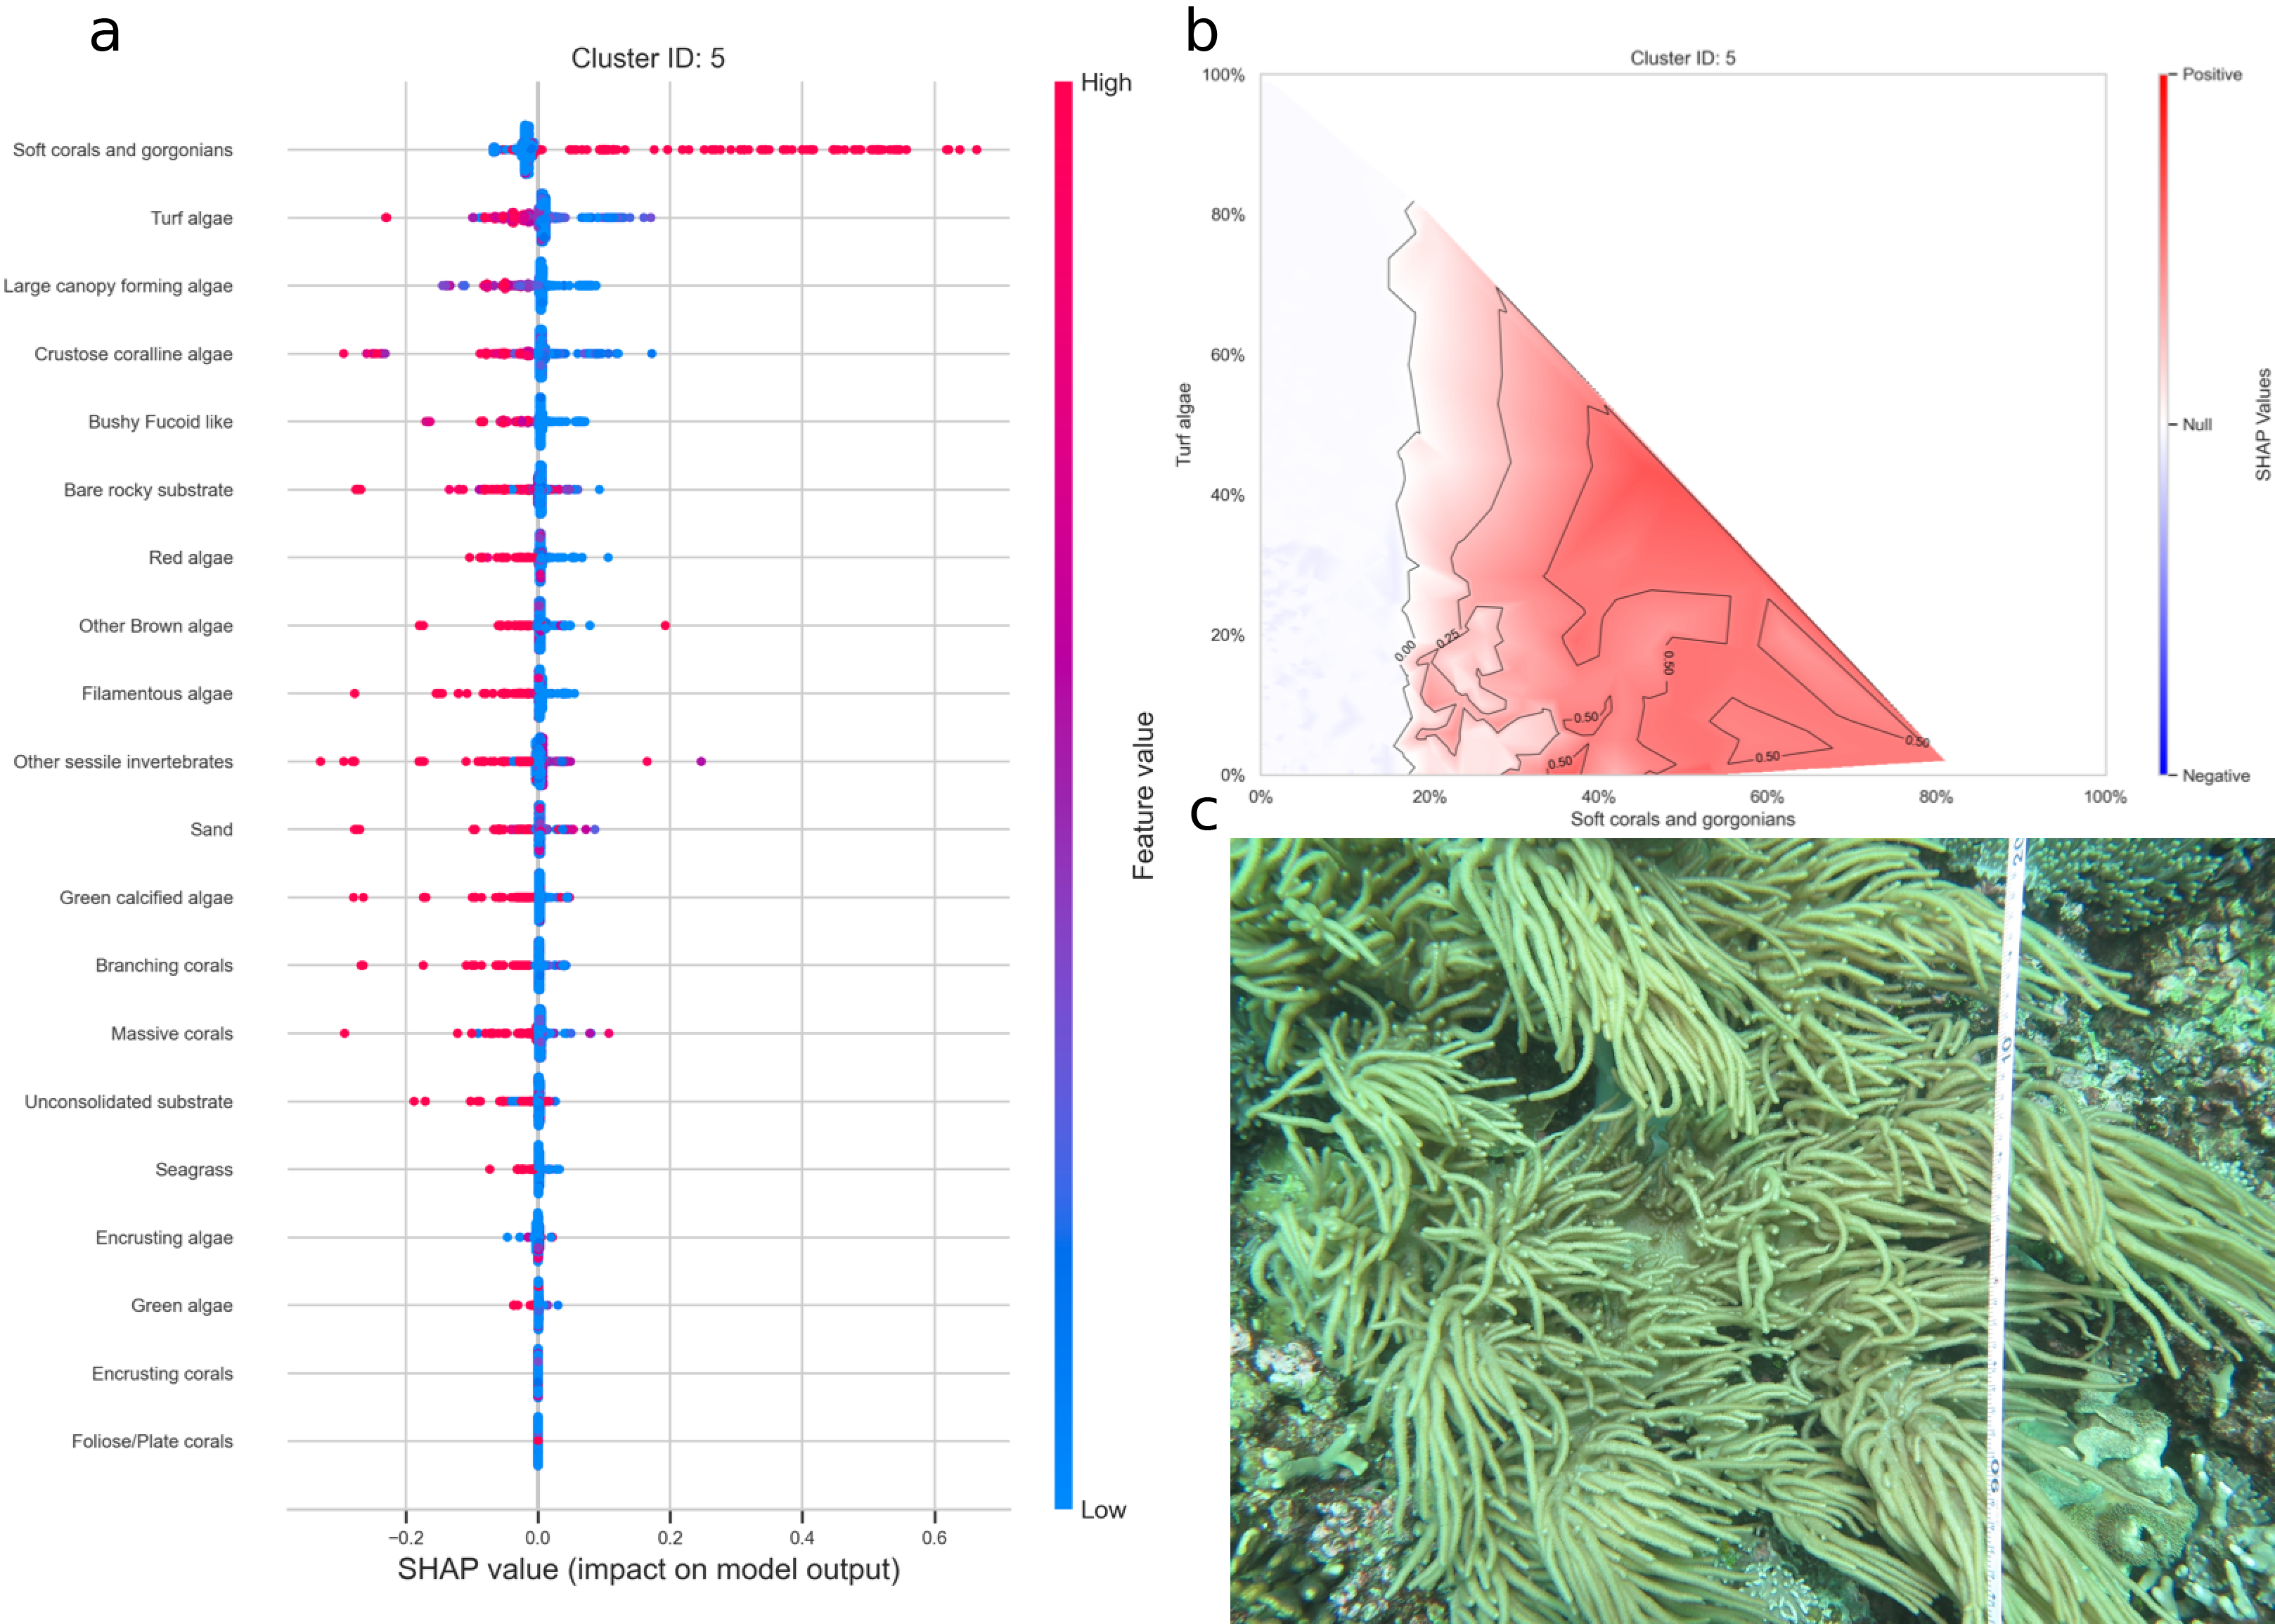
\includegraphics{03-Chapitre2/figures/supplementary/05-explanation_shap_pq_cluster_5.png}
\caption{a. \emph{SHAP} summary plot showing the impact of each habitat
substrate on the classification. The position of each habitat group on
the y-axis indicates its relative importance for the considered cluster.
The position of each point along the x-axis indicates if the observation
is associated with a lower or higher affinity with the cluster and the
colour of the point indicates if the value of the cover of this habitat
is rather high or low. b. Linear interpolation of the \emph{SHAP} values
for the two most influential variables for the cluster \emph{soft coral
and gorgonians}. c.~Example of photoquadrat for one transect of the
cluster \emph{soft coral and gorgonians} categorised by \emph{HDBSCAN}
as exemplary.}\label{fig:chap2figS25}
}
\end{figure}

\begin{figure}
\hypertarget{fig:26}{%
\centering
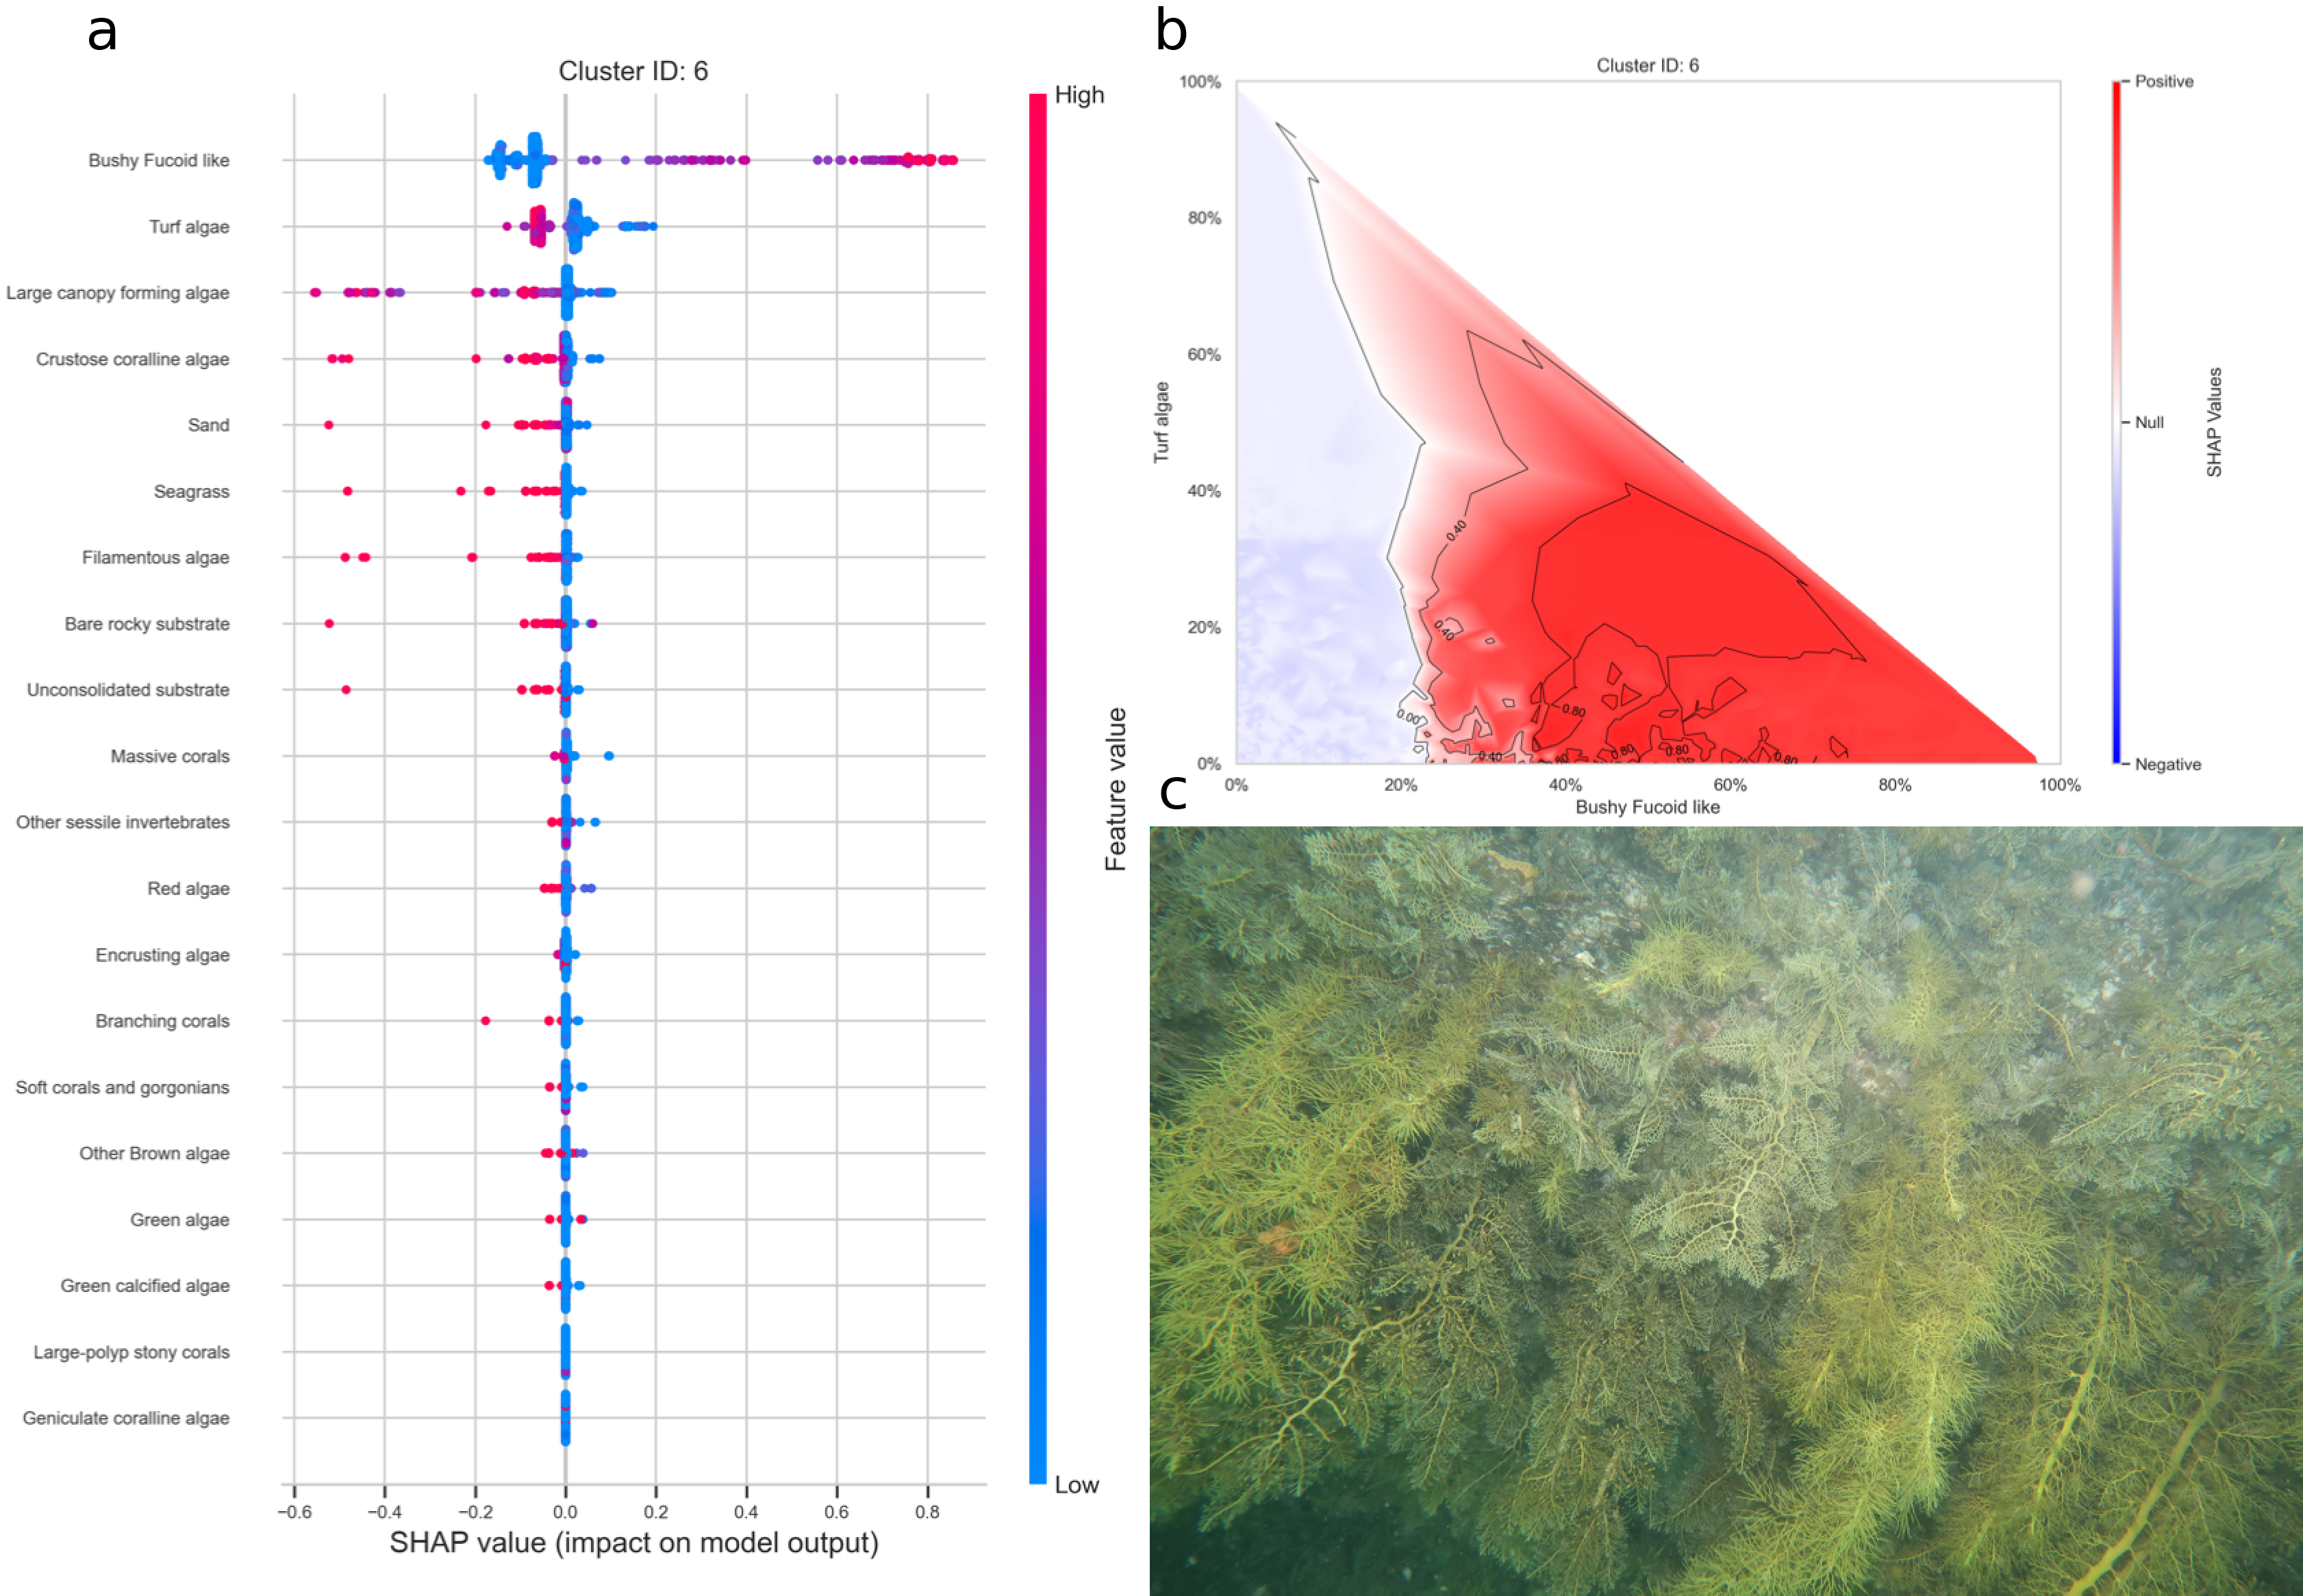
\includegraphics{03-Chapitre2/figures/supplementary/05-explanation_shap_pq_cluster_6.png}
\caption{a. \emph{SHAP} summary plot showing the impact of each habitat
substrate on the classification. The position of each habitat group on
the y-axis indicates its relative importance for the considered cluster.
The position of each point along the x-axis indicates if the observation
is associated with a lower or higher affinity with the cluster and the
colour of the point indicates if the value of the cover of this habitat
is rather high or low. b. Linear interpolation of the \emph{SHAP} values
for the two most influential variables for the cluster \emph{bushy
fucoid-like}. c.~Example of photoquadrat for one transect of the cluster
\emph{bushy fucoid-like} categorised by \emph{HDBSCAN} as
exemplary.}\label{fig:26}
}
\end{figure}

\begin{figure}
\hypertarget{fig:chap2figS27}{%
\centering
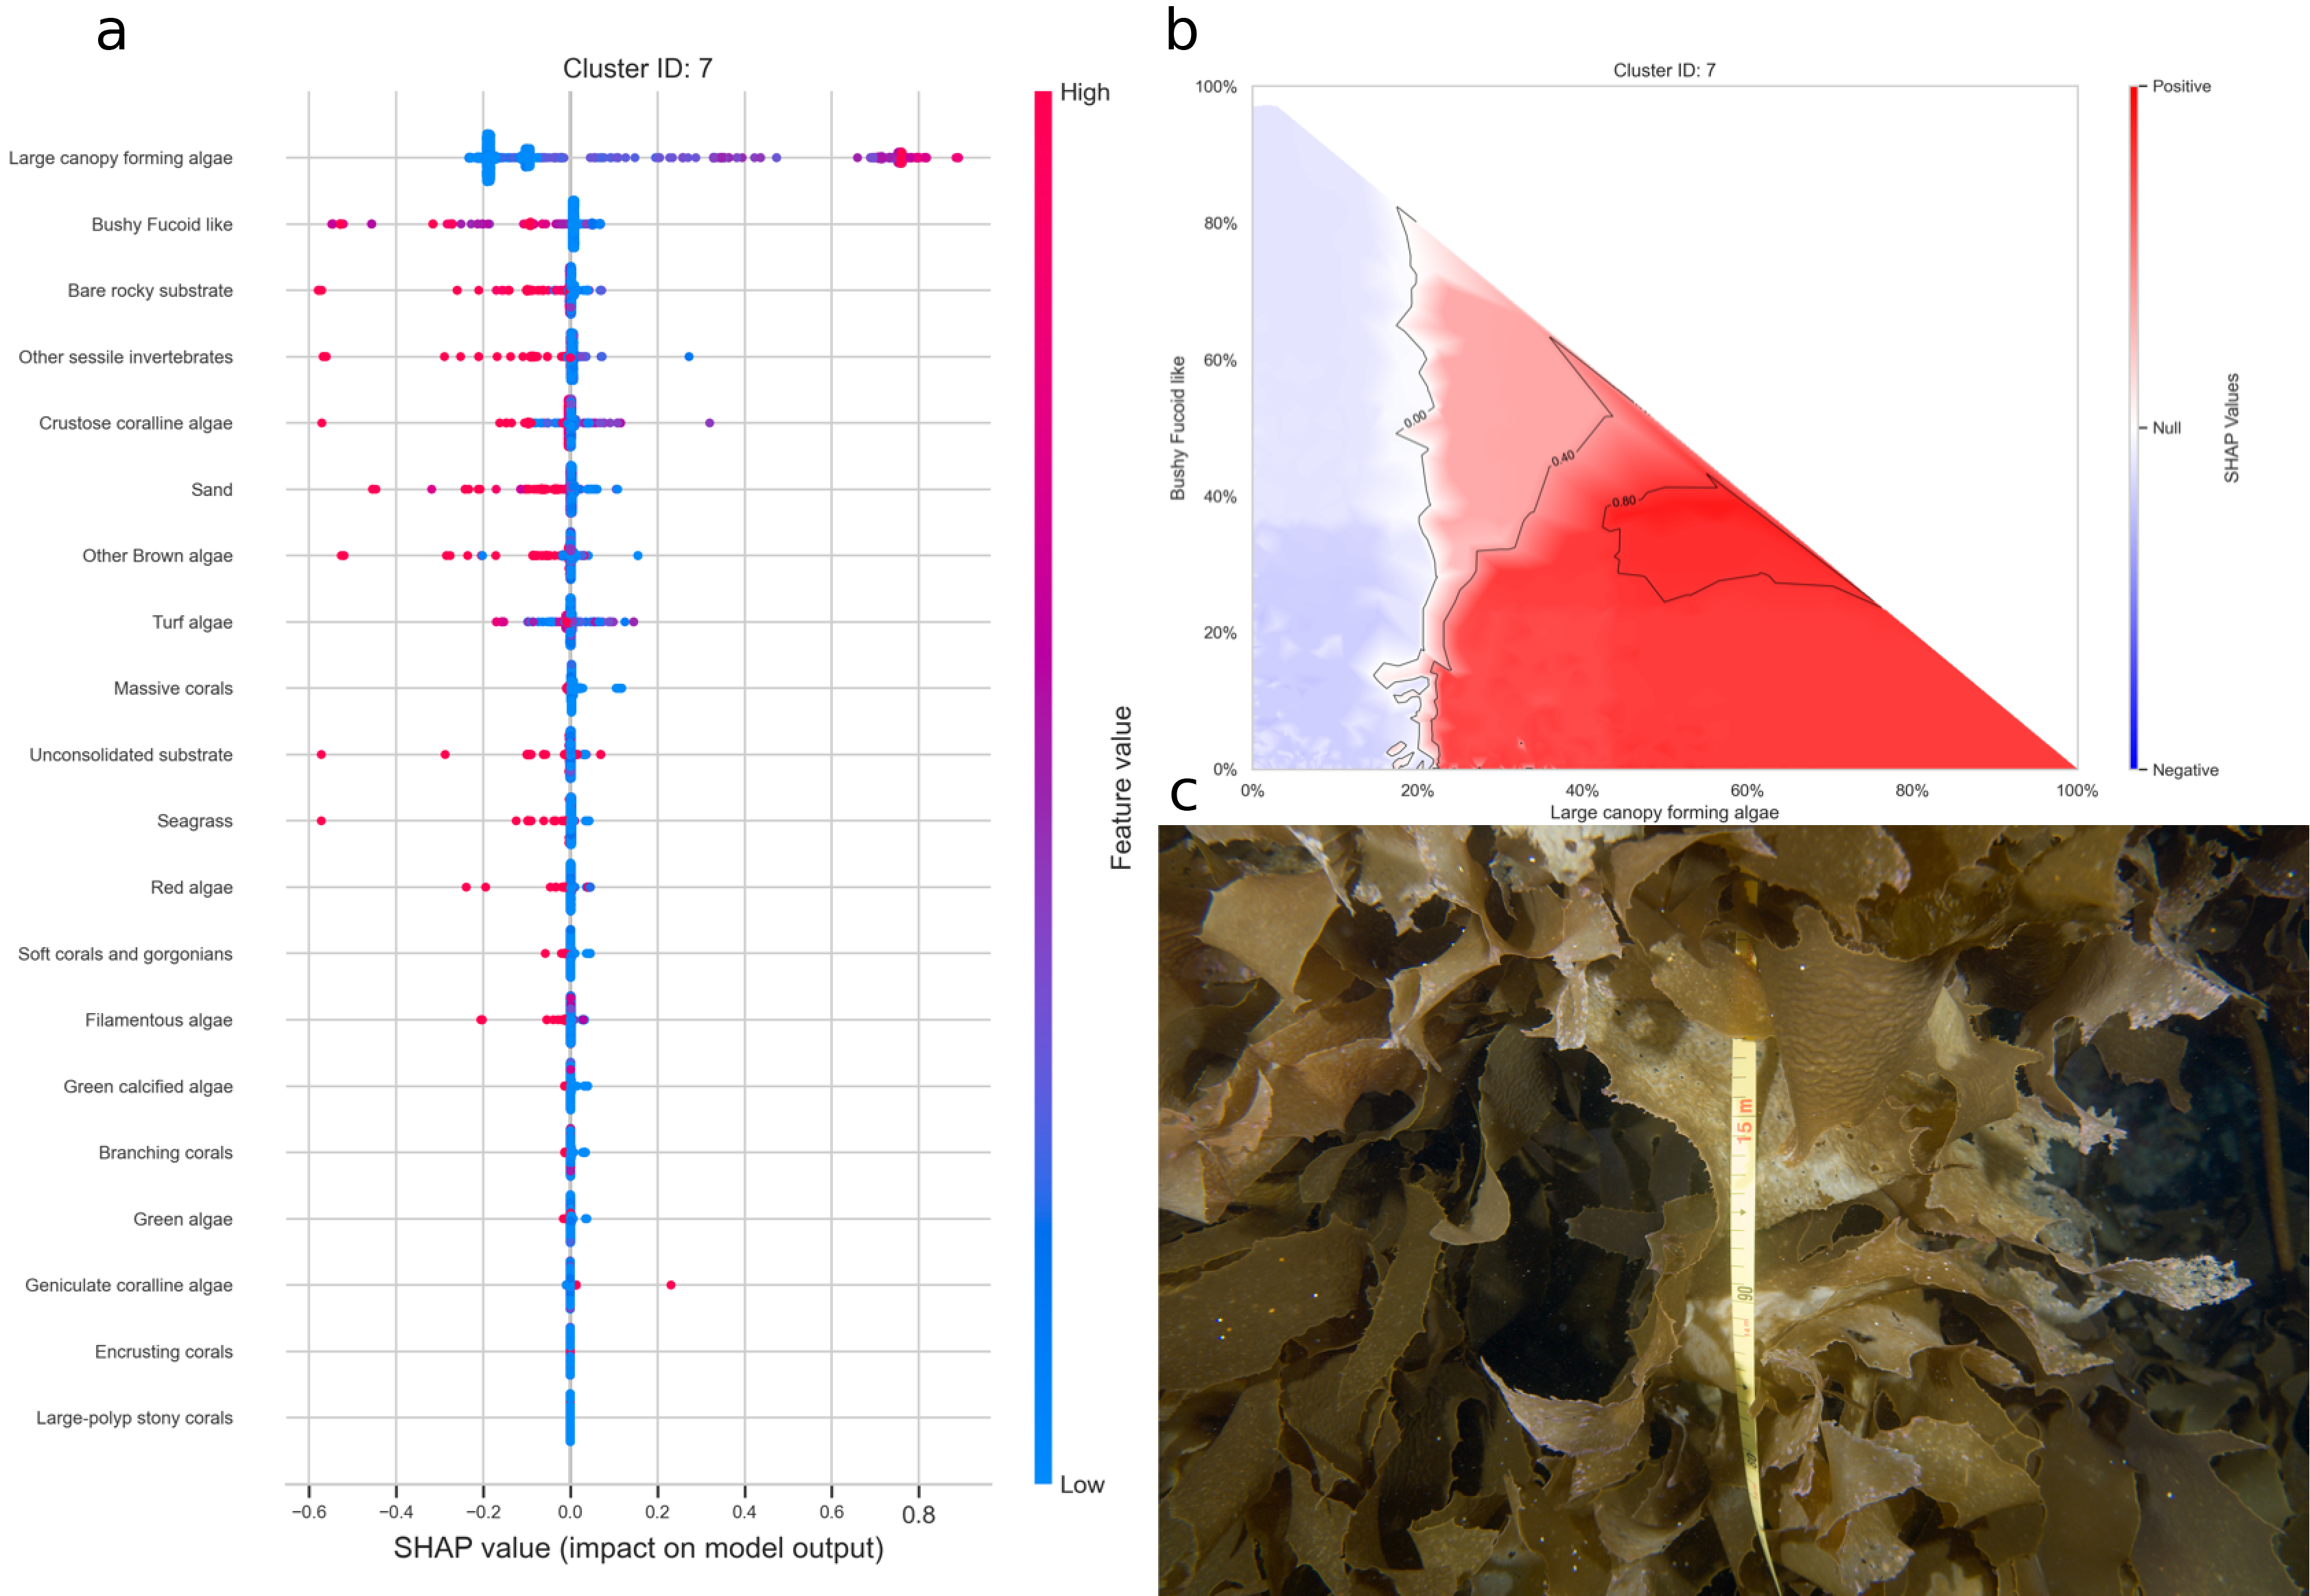
\includegraphics{03-Chapitre2/figures/supplementary/05-explanation_shap_pq_cluster_7.png}
\caption{a. \emph{SHAP} summary plot showing the impact of each habitat
substrate on the classification. The position of each habitat group on
the y-axis indicates its relative importance for the considered cluster.
The position of each point along the x-axis indicates if the observation
is associated with a lower or higher affinity with the cluster and the
colour of the point indicates if the value of the cover of this habitat
is rather high or low. b. Linear interpolation of the \emph{SHAP} values
for the two most influential variables for the cluster \emph{large
canopy forming algae}. c.~Example of photoquadrat for one transect of
the cluster \emph{large canopy forming algae} categorised by
\emph{HDBSCAN} as exemplary.}\label{fig:chap2figS27}
}
\end{figure}

\begin{figure}
\hypertarget{fig:chap2figS28}{%
\centering
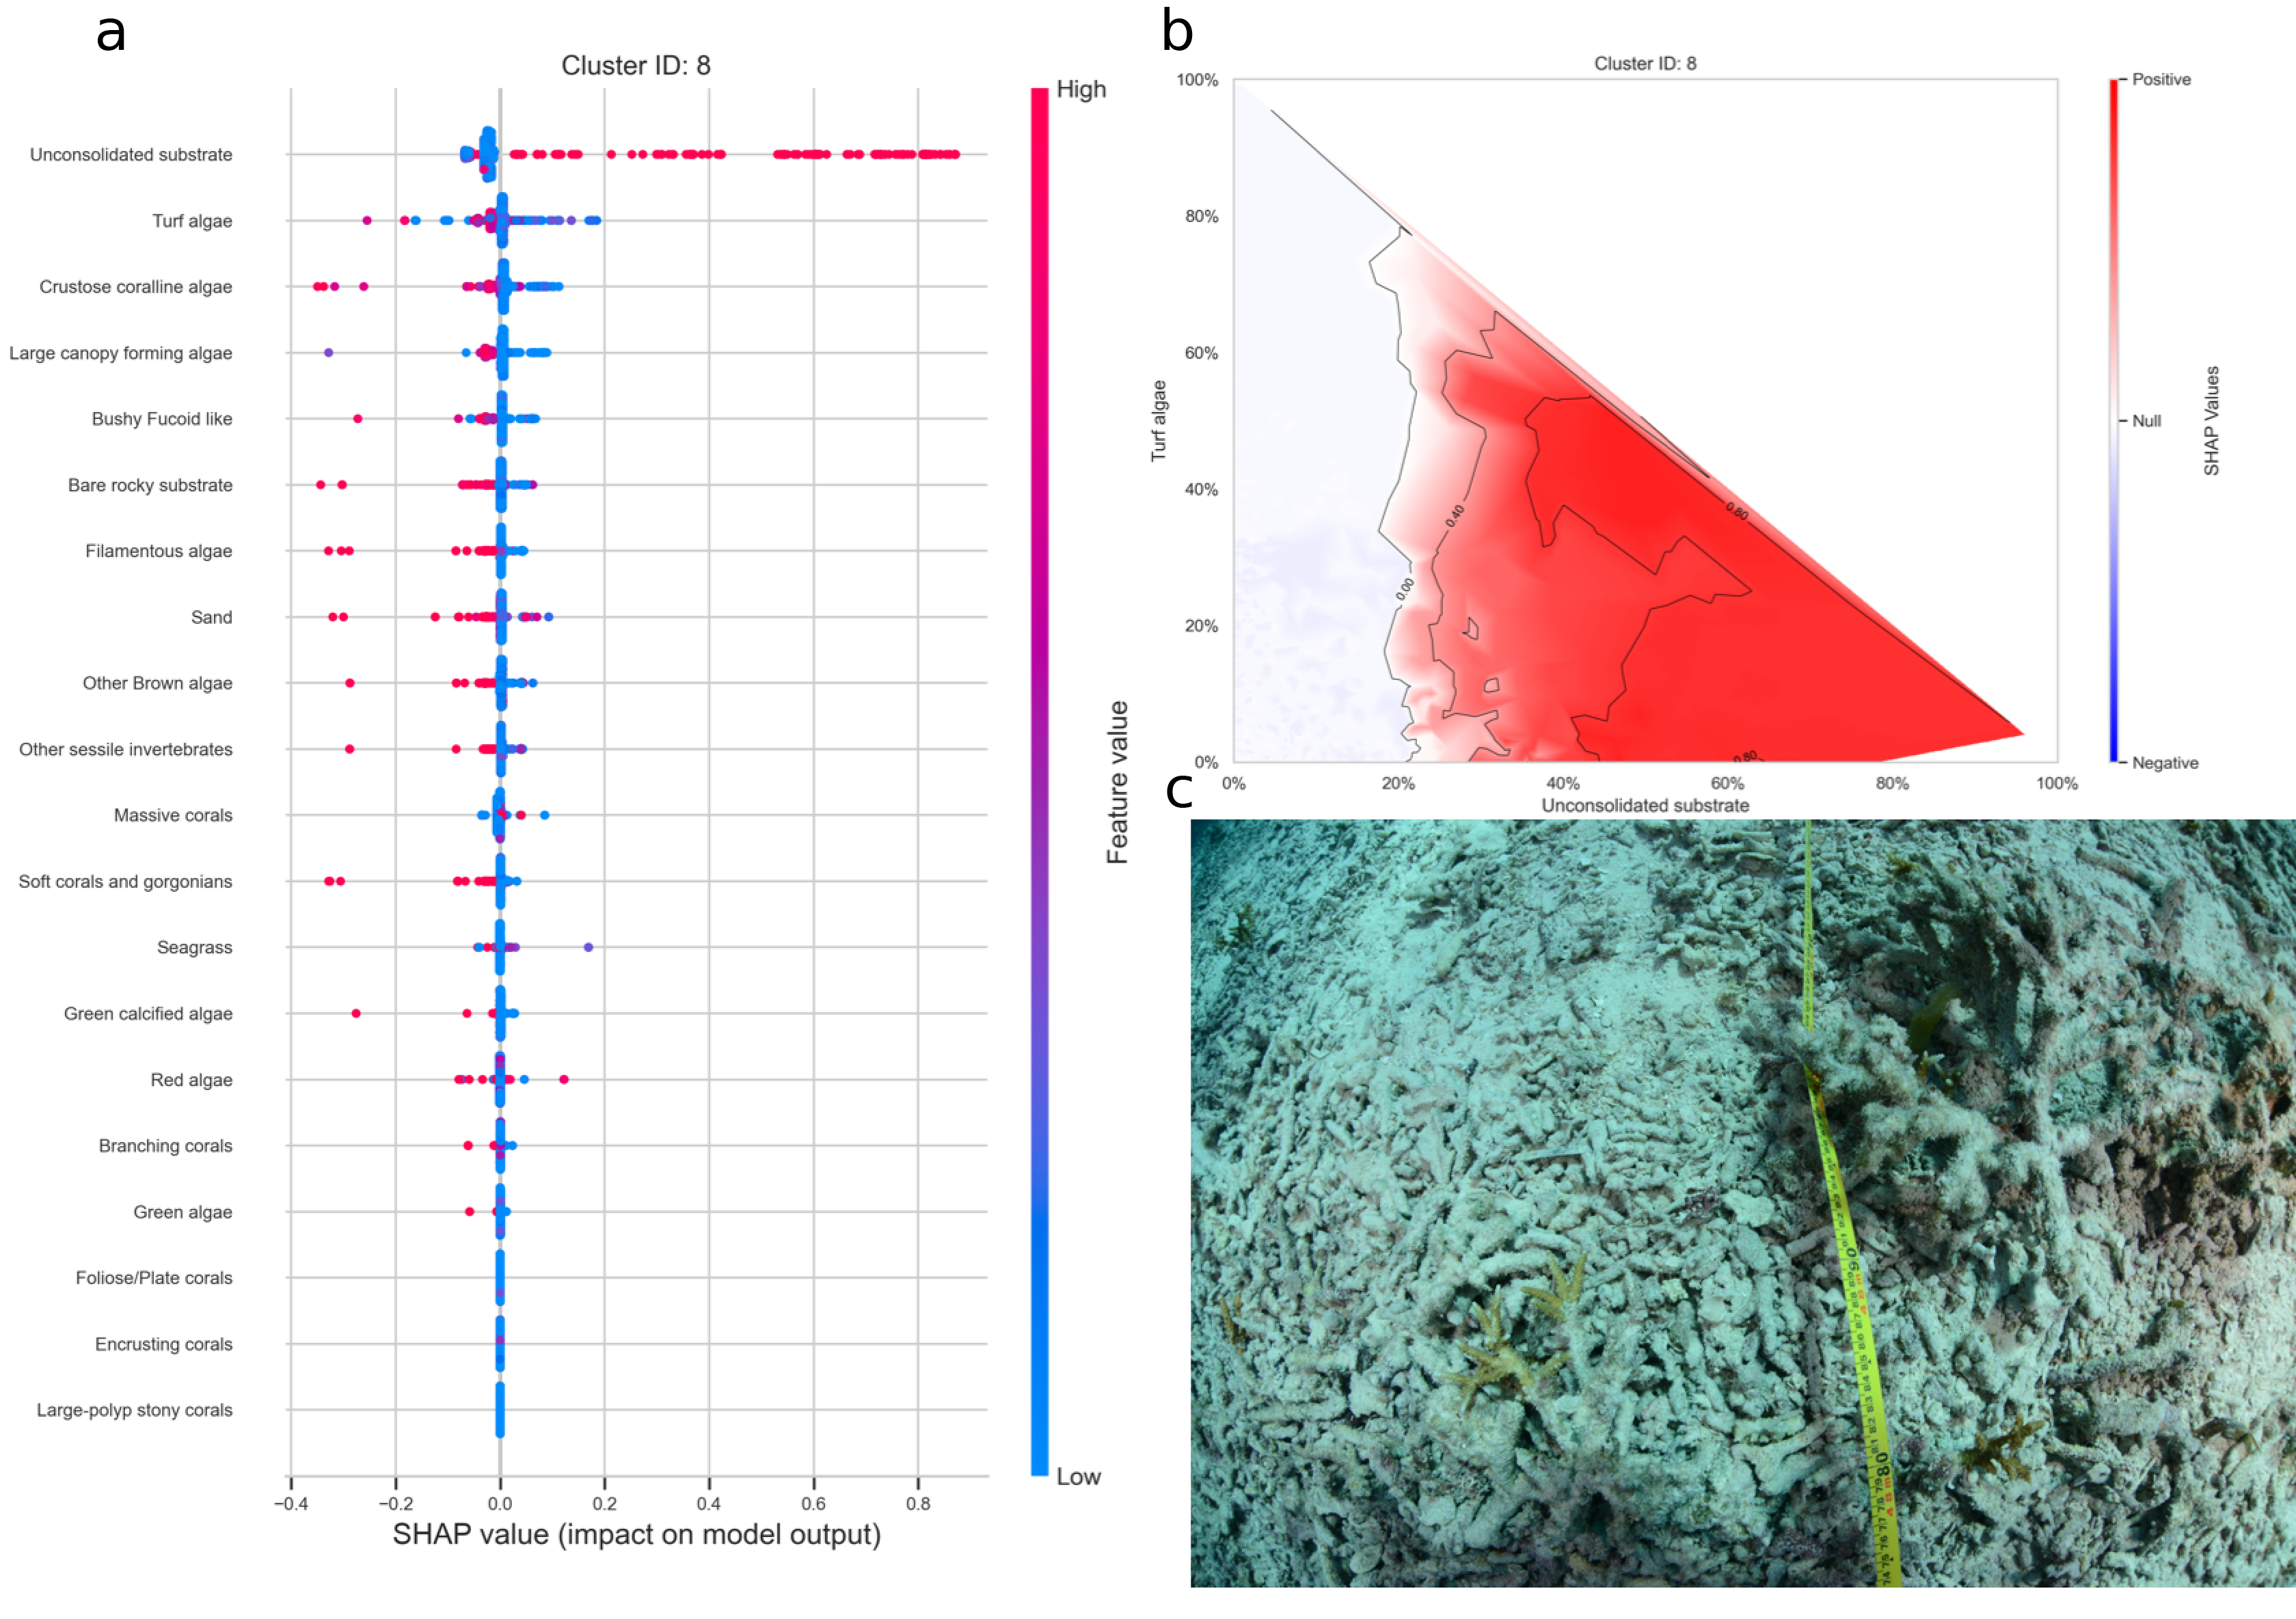
\includegraphics{03-Chapitre2/figures/supplementary/05-explanation_shap_pq_cluster_8.png}
\caption{a. \emph{SHAP} summary plot showing the impact of each habitat
substrate on the classification. The position of each habitat group on
the y-axis indicates its relative importance for the considered cluster.
The position of each point along the x-axis indicates if the observation
is associated with a lower or higher affinity with the cluster and the
colour of the point indicates if the value of the cover of this habitat
is rather high or low. b. Linear interpolation of the \emph{SHAP} values
for the two most influential variables for the cluster
\emph{unconsolidated substrat}. c.~Example of photoquadrat for one
transect of the cluster \emph{unconsolidated substrat} categorised by
\emph{HDBSCAN} as exemplary.}\label{fig:chap2figS28}
}
\end{figure}

\begin{figure}
\hypertarget{fig:chap2figS29}{%
\centering
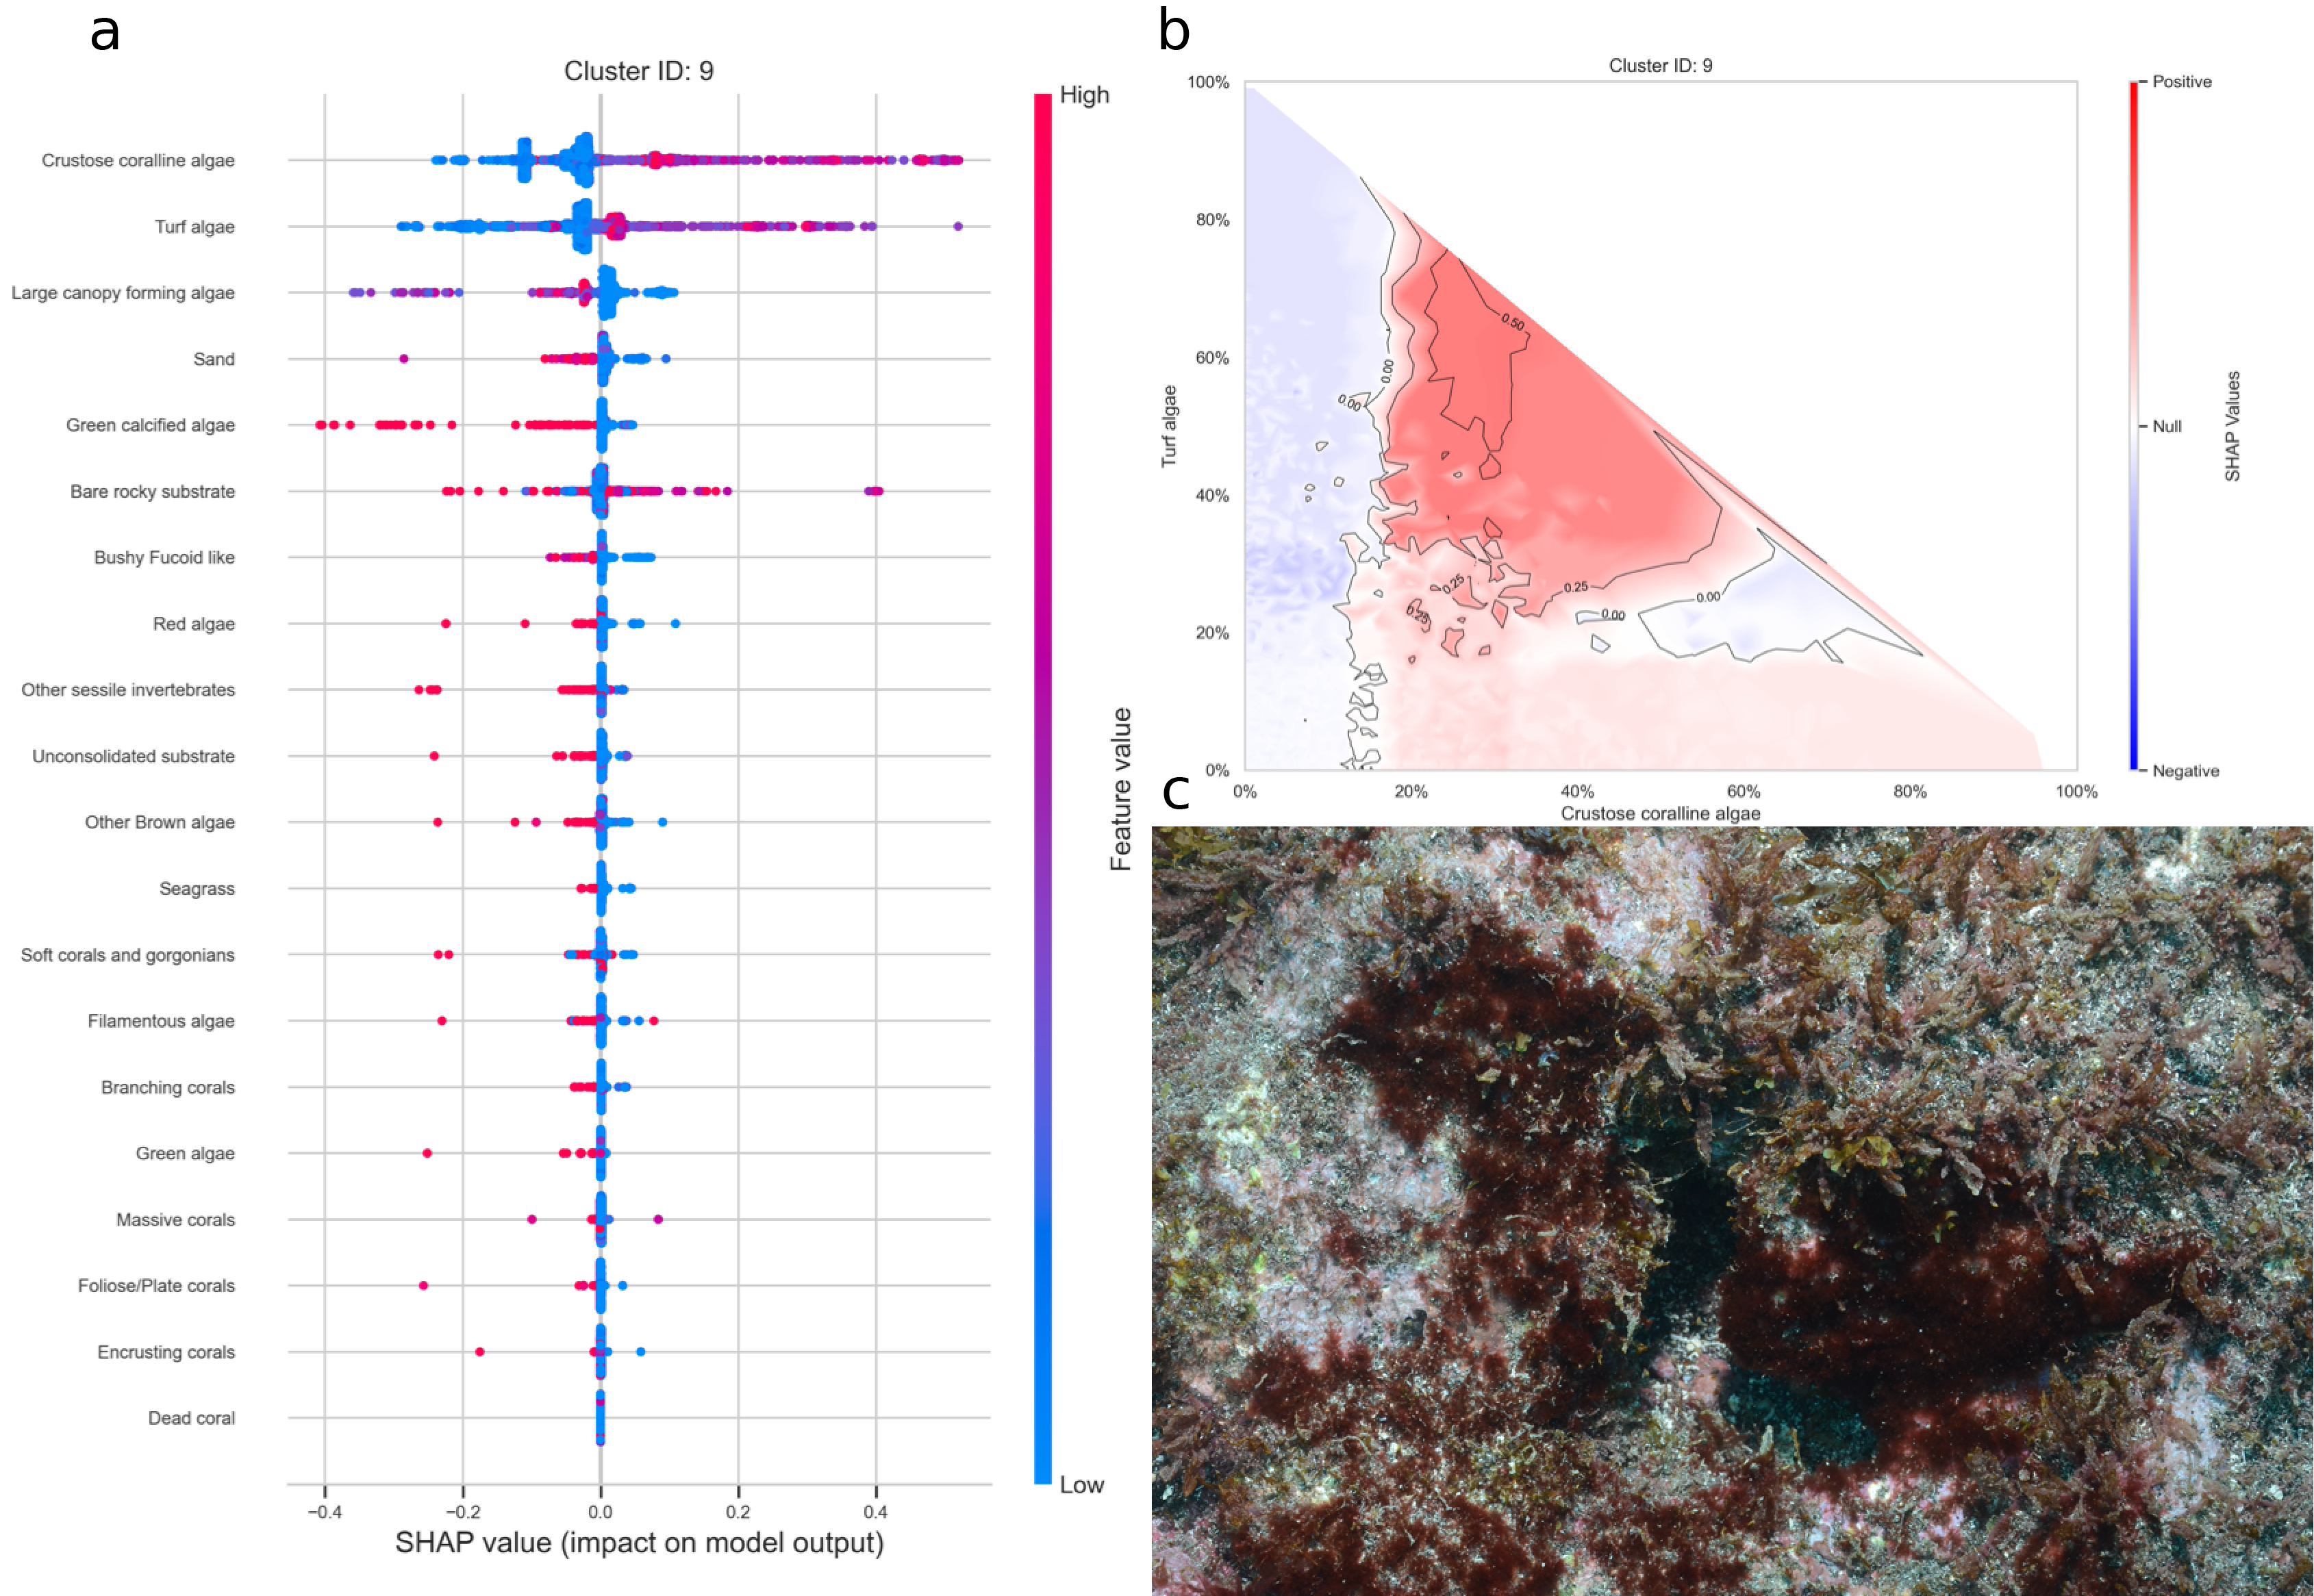
\includegraphics{03-Chapitre2/figures/supplementary/05-explanation_shap_pq_cluster_9.png}
\caption{a. \emph{SHAP} summary plot showing the impact of each habitat
substrate on the classification. The position of each habitat group on
the y-axis indicates its relative importance for the considered cluster.
The position of each point along the x-axis indicates if the observation
is associated with a lower or higher affinity with the cluster and the
colour of the point indicates if the value of the cover of this habitat
is rather high or low. b. Linear interpolation of the \emph{SHAP} values
for the two most influential variables for the cluster \emph{crustose
coralline algae and turf}. c.~Example of photoquadrat for one transect
of the cluster \emph{crustose coralline algae and turf} categorised by
\emph{HDBSCAN} as exemplary.}\label{fig:chap2figS29}
}
\end{figure}

\begin{figure}
\hypertarget{fig:chap2figS30}{%
\centering
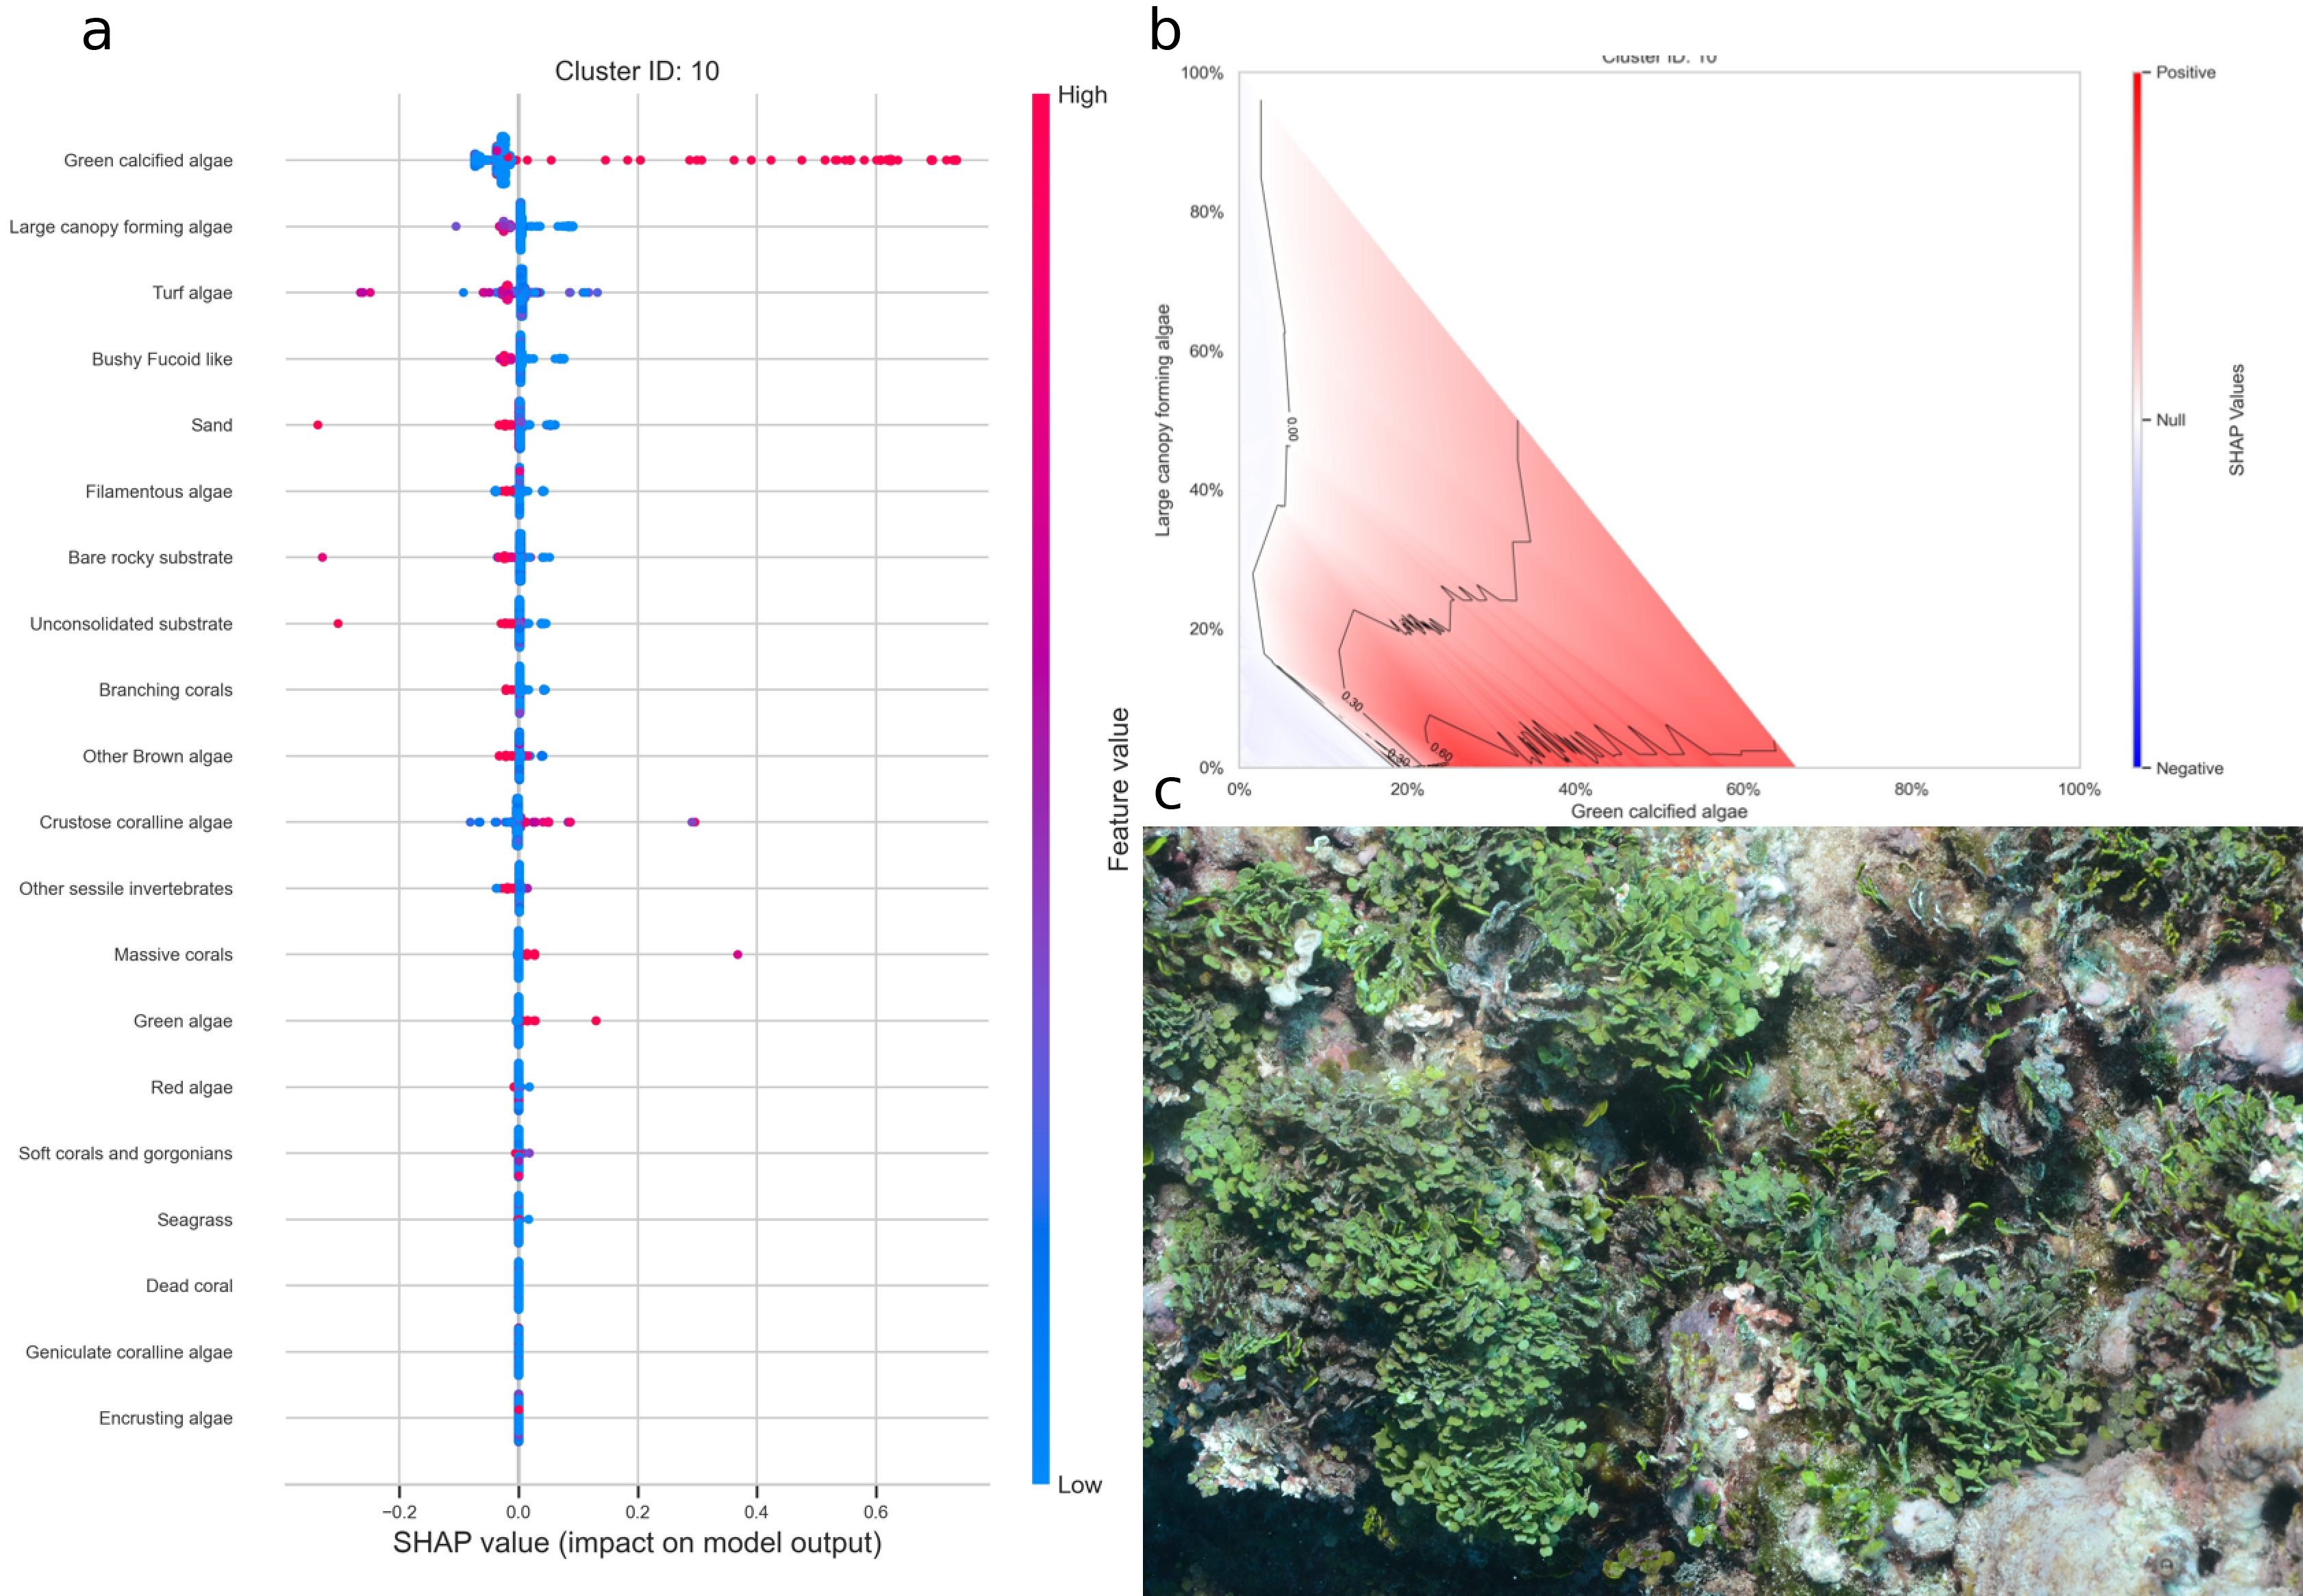
\includegraphics{03-Chapitre2/figures/supplementary/05-explanation_shap_pq_cluster_10.png}
\caption{a. \emph{SHAP} summary plot showing the impact of each habitat
substrate on the classification. The position of each habitat group on
the y-axis indicates its relative importance for the considered cluster.
The position of each point along the x-axis indicates if the observation
is associated with a lower or higher affinity with the cluster and the
colour of the point indicates if the value of the cover of this habitat
is rather high or low. b. Linear interpolation of the \emph{SHAP} values
for the two most influential variables for the cluster \emph{green
calcified algae}. c.~Example of photoquadrat for one transect of the
cluster \emph{green calcified algae} categorised by \emph{HDBSCAN} as
exemplary.}\label{fig:chap2figS30}
}
\end{figure}

\begin{figure}
\hypertarget{fig:chap2figS31}{%
\centering
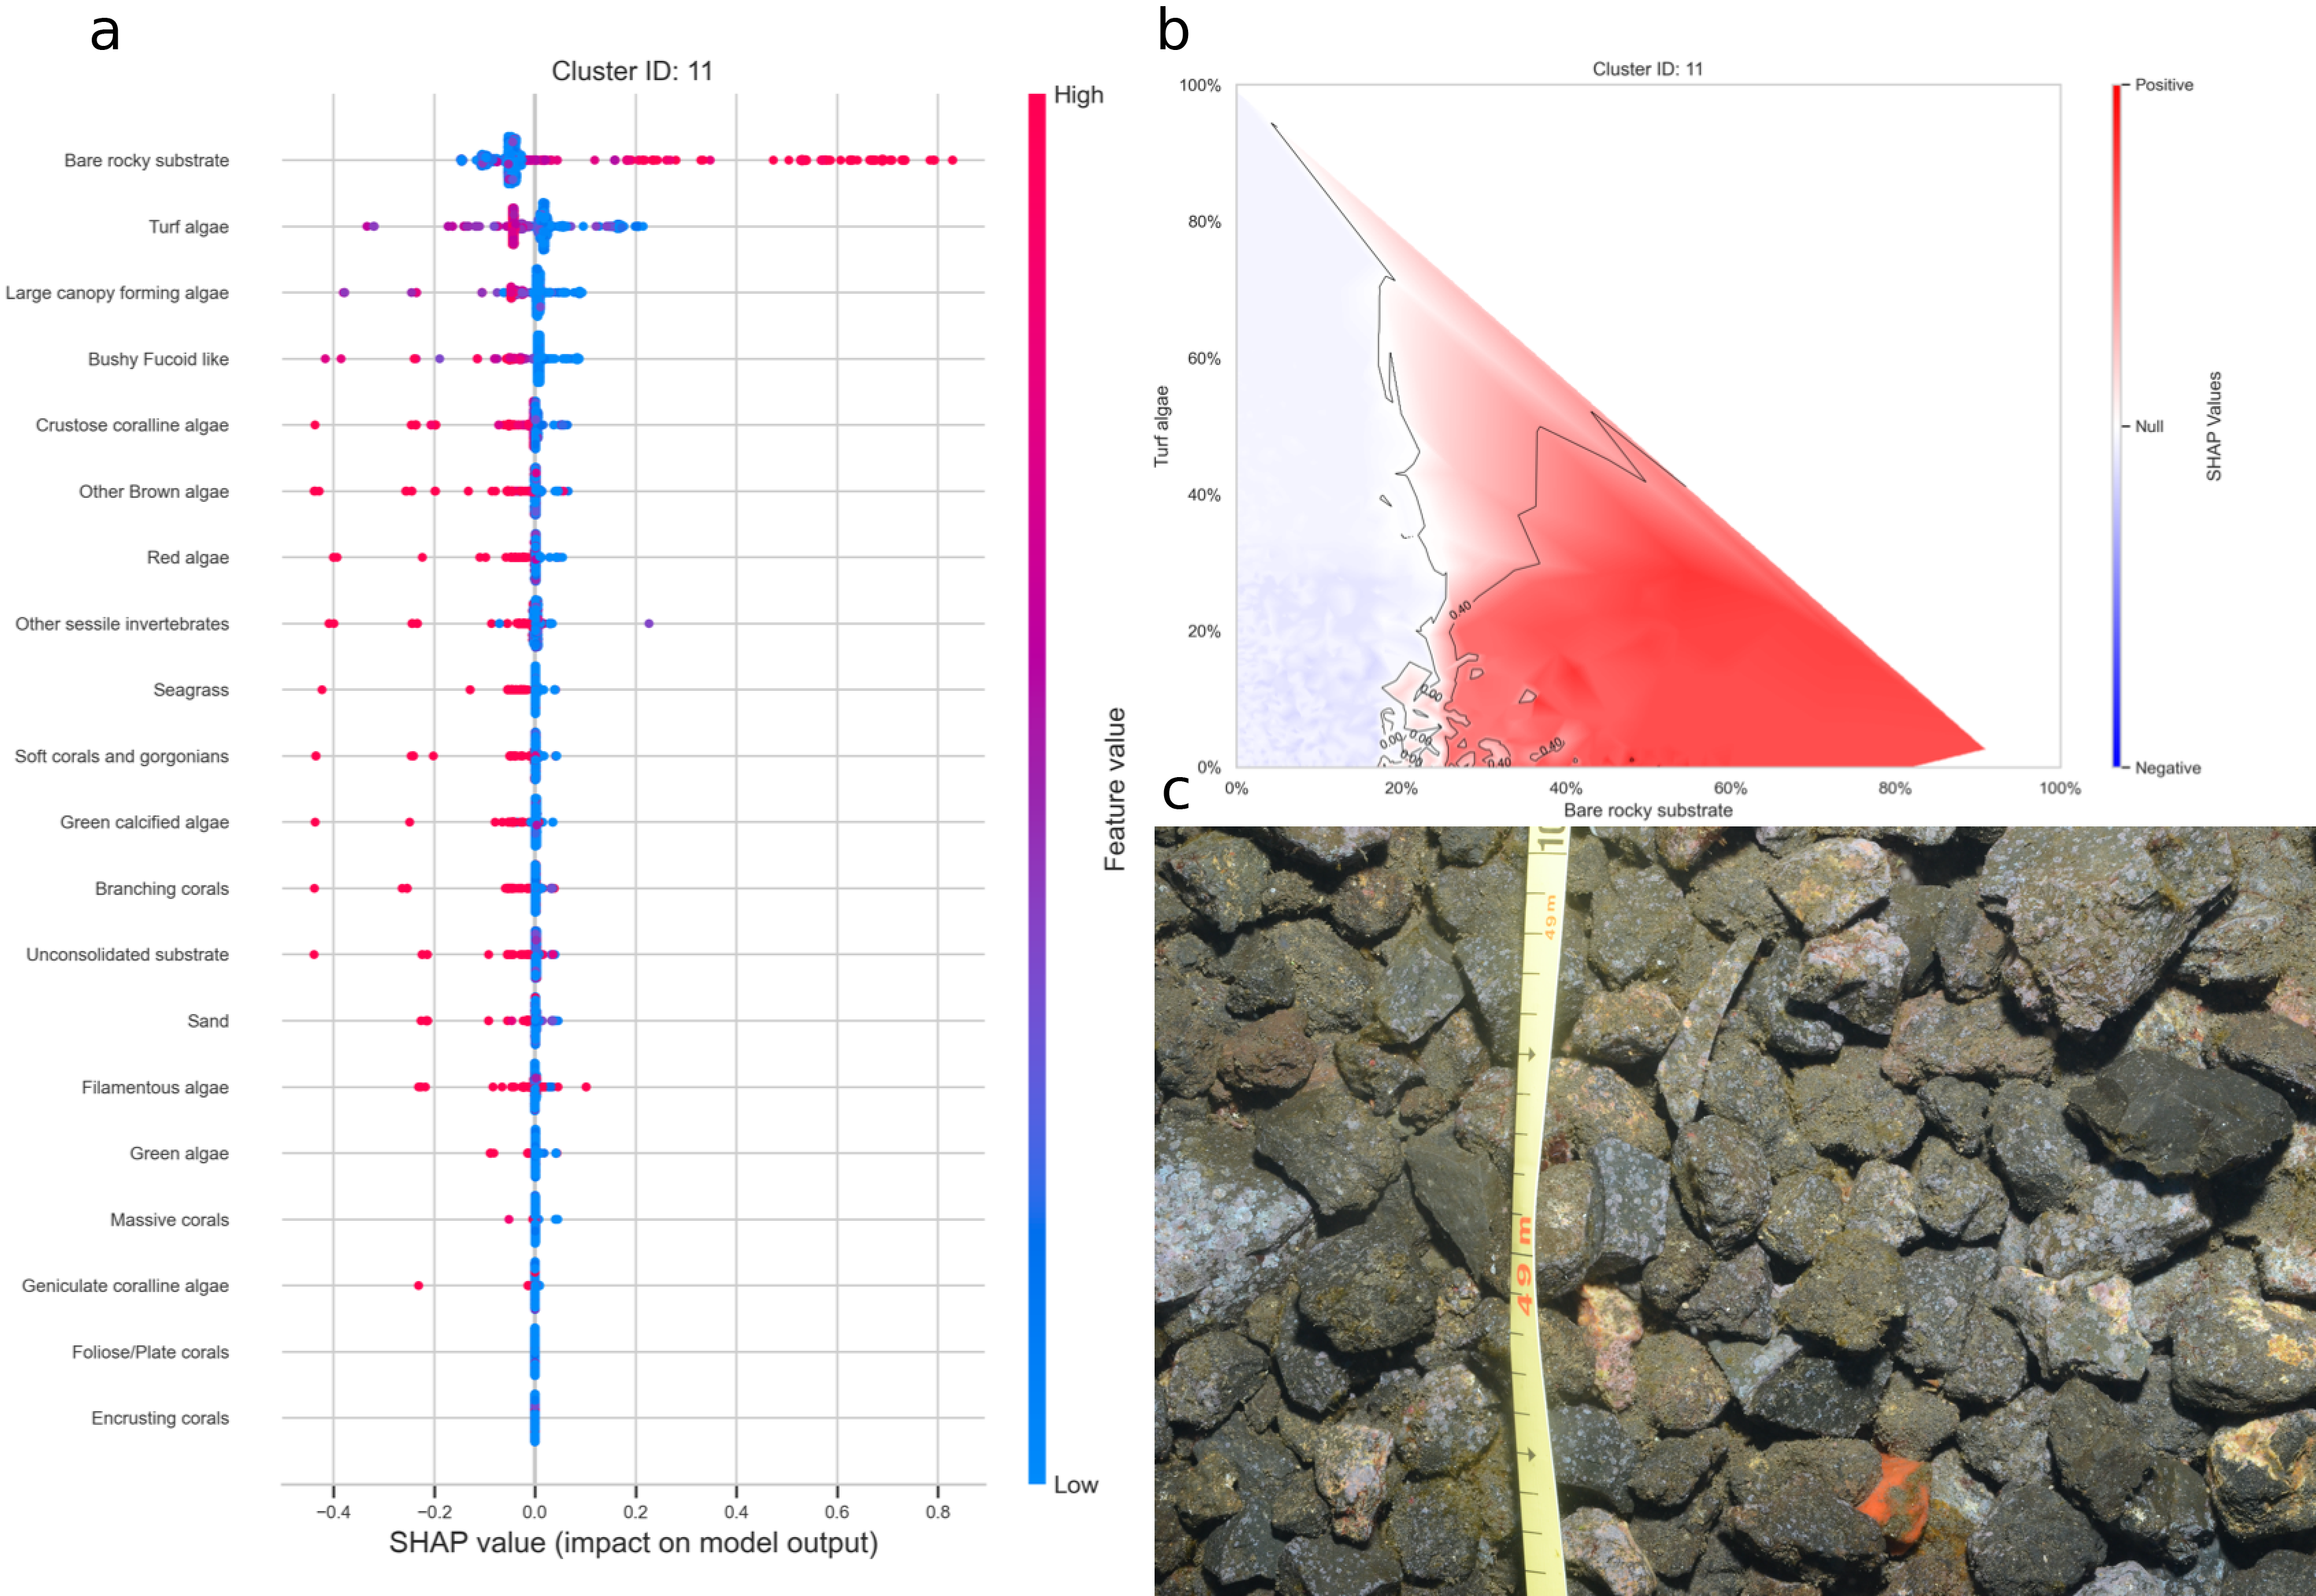
\includegraphics{03-Chapitre2/figures/supplementary/05-explanation_shap_pq_cluster_11.png}
\caption{a. \emph{SHAP} summary plot showing the impact of each habitat
substrate on the classification. The position of each habitat group on
the y-axis indicates its relative importance for the considered cluster.
The position of each point along the x-axis indicates if the observation
is associated with a lower or higher affinity with the cluster and the
colour of the point indicates if the value of the cover of this habitat
is rather high or low. b. Linear interpolation of the \emph{SHAP} values
for the two most influential variables for the cluster \emph{bare
substrate}. c.~Example of photoquadrat for one transect of the cluster
\emph{bare substrate} categorised by \emph{HDBSCAN} as
exemplary.}\label{fig:chap2figS31}
}
\end{figure}

\begin{figure}
\hypertarget{fig:chap2figS32}{%
\centering
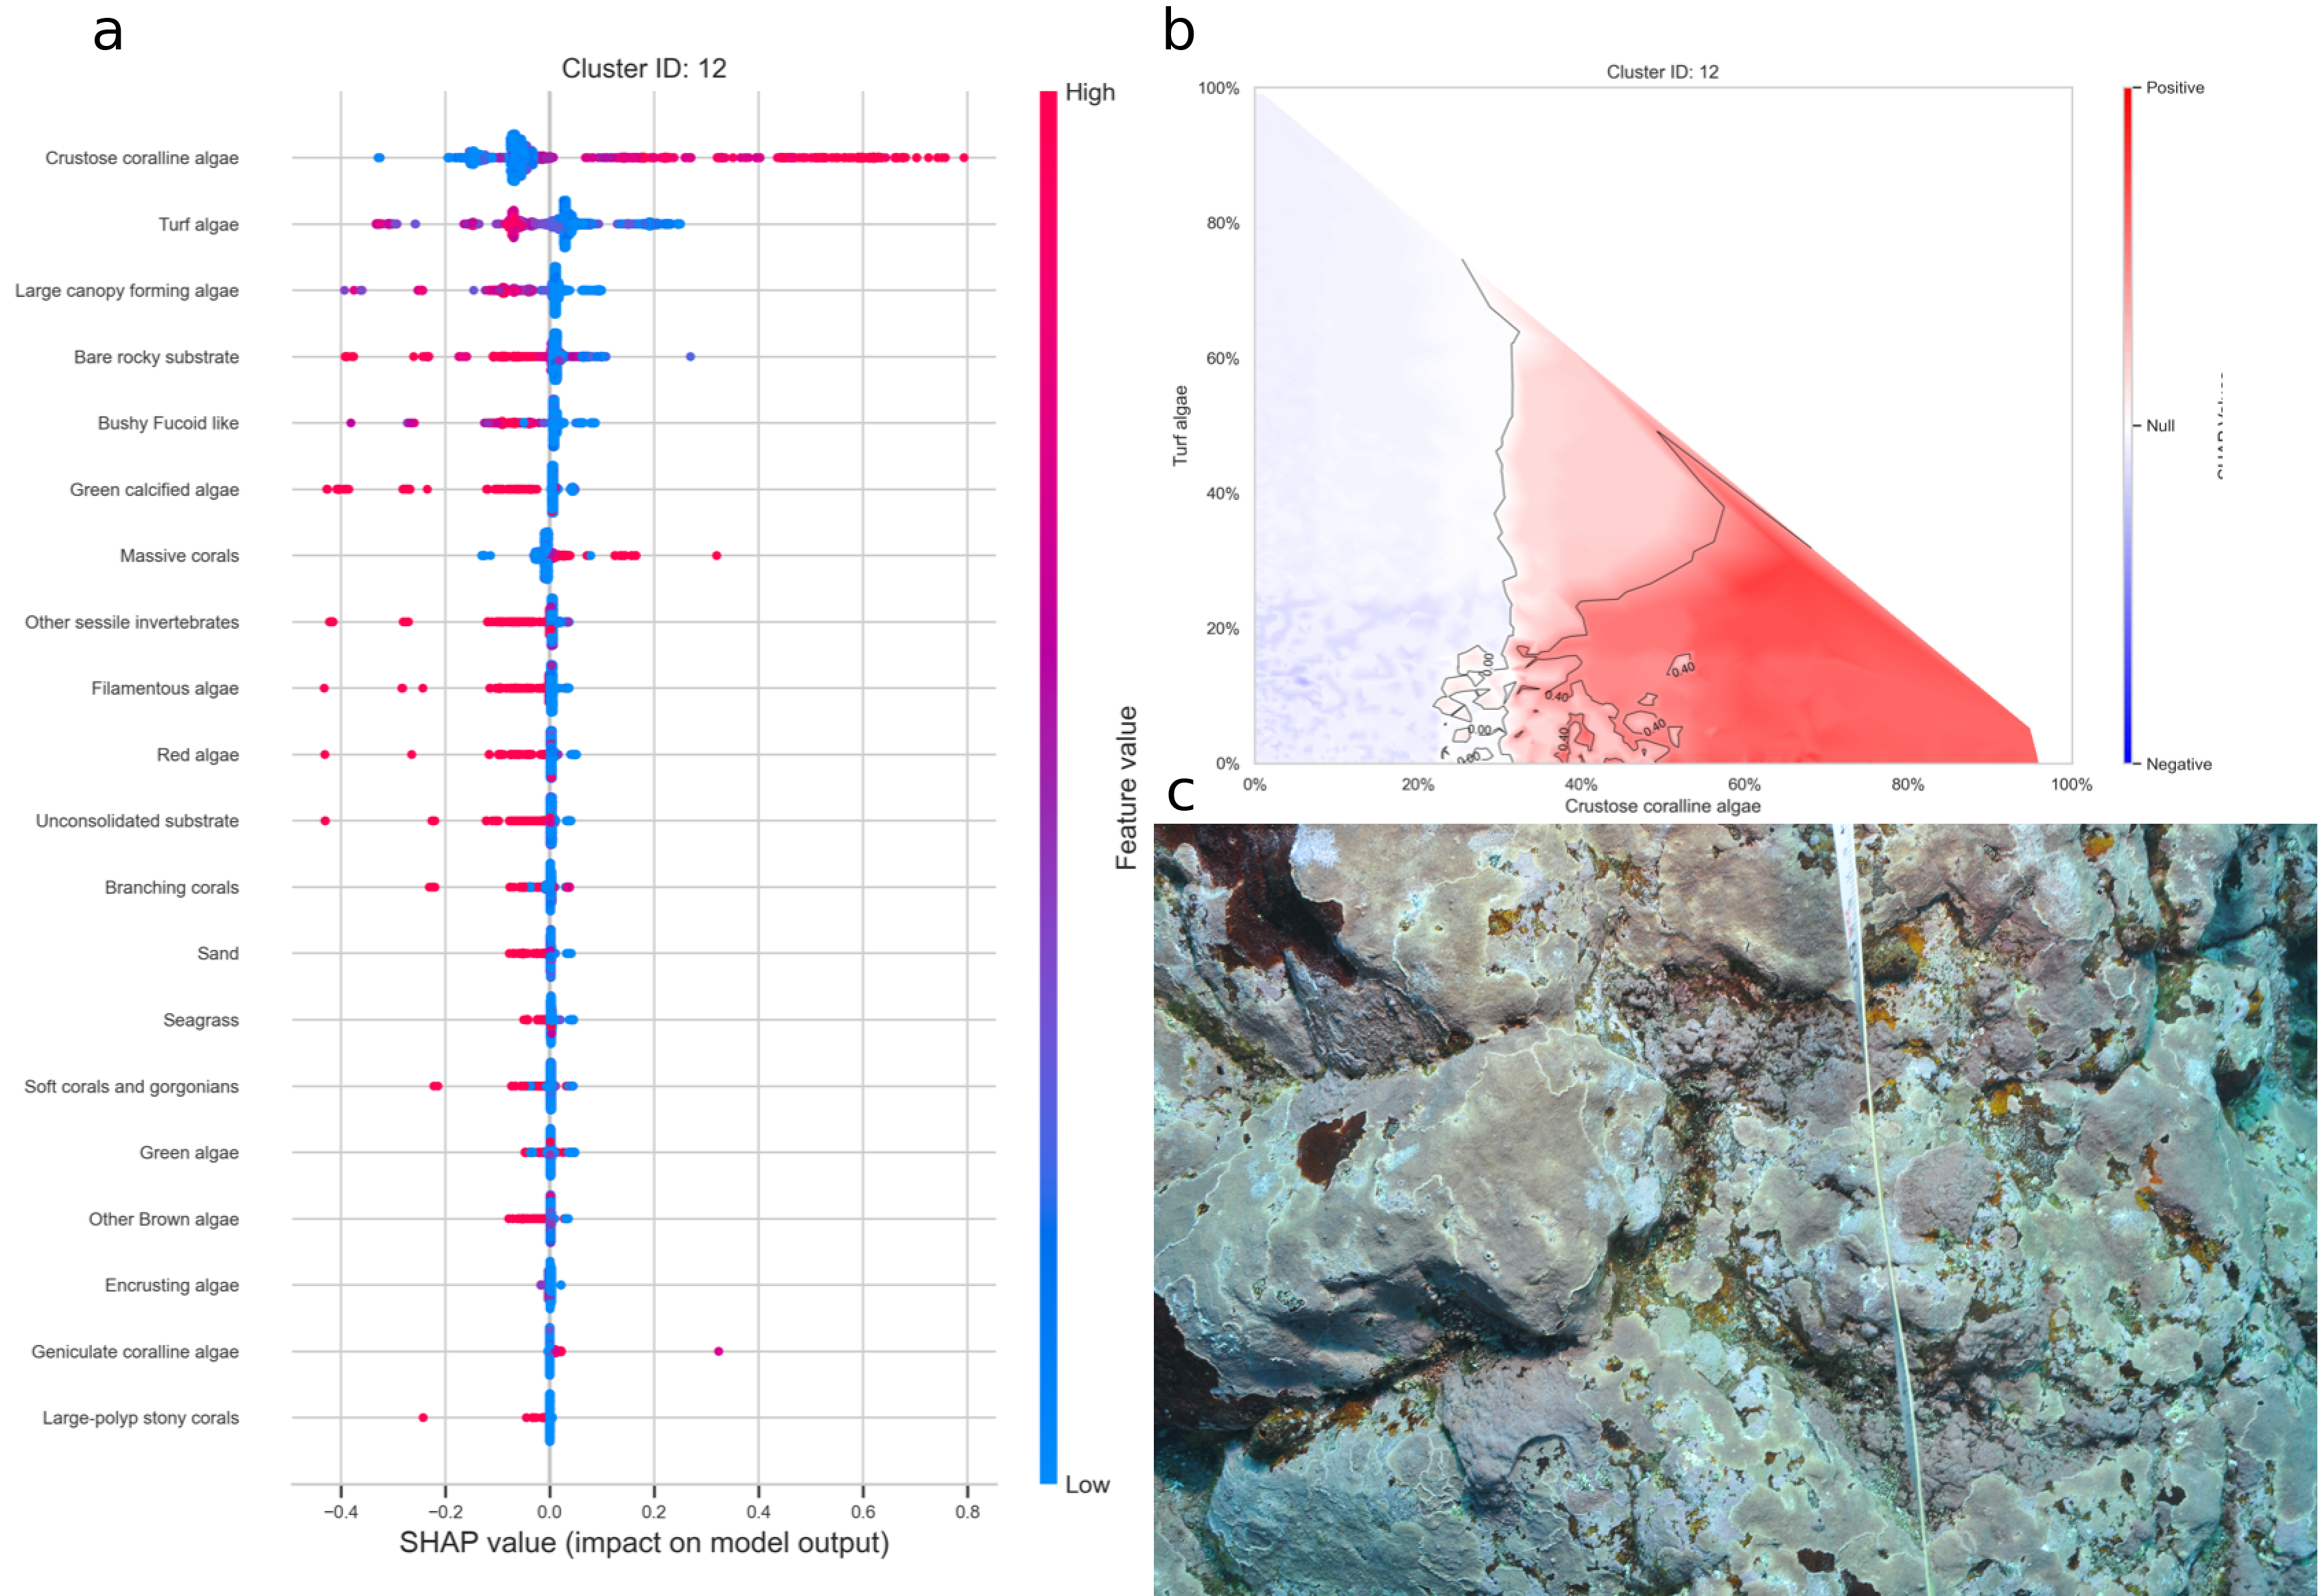
\includegraphics{03-Chapitre2/figures/supplementary/05-explanation_shap_pq_cluster_12.png}
\caption{a. \emph{SHAP} summary plot showing the impact of each habitat
substrate on the classification. The position of each habitat group on
the y-axis indicates its relative importance for the considered cluster.
The position of each point along the x-axis indicates if the observation
is associated with a lower or higher affinity with the cluster and the
colour of the point indicates if the value of the cover of this habitat
is rather high or low. b. Linear interpolation of the \emph{SHAP} values
for the two most influential variables for the cluster \emph{crustose
coralline algae}. c.~Example of photoquadrat for one transect of the
cluster \emph{crustose coralline algae} categorised by \emph{HDBSCAN} as
exemplary.}\label{fig:chap2figS32}
}
\end{figure}

\begin{figure}
\hypertarget{fig:chap2figS33}{%
\centering
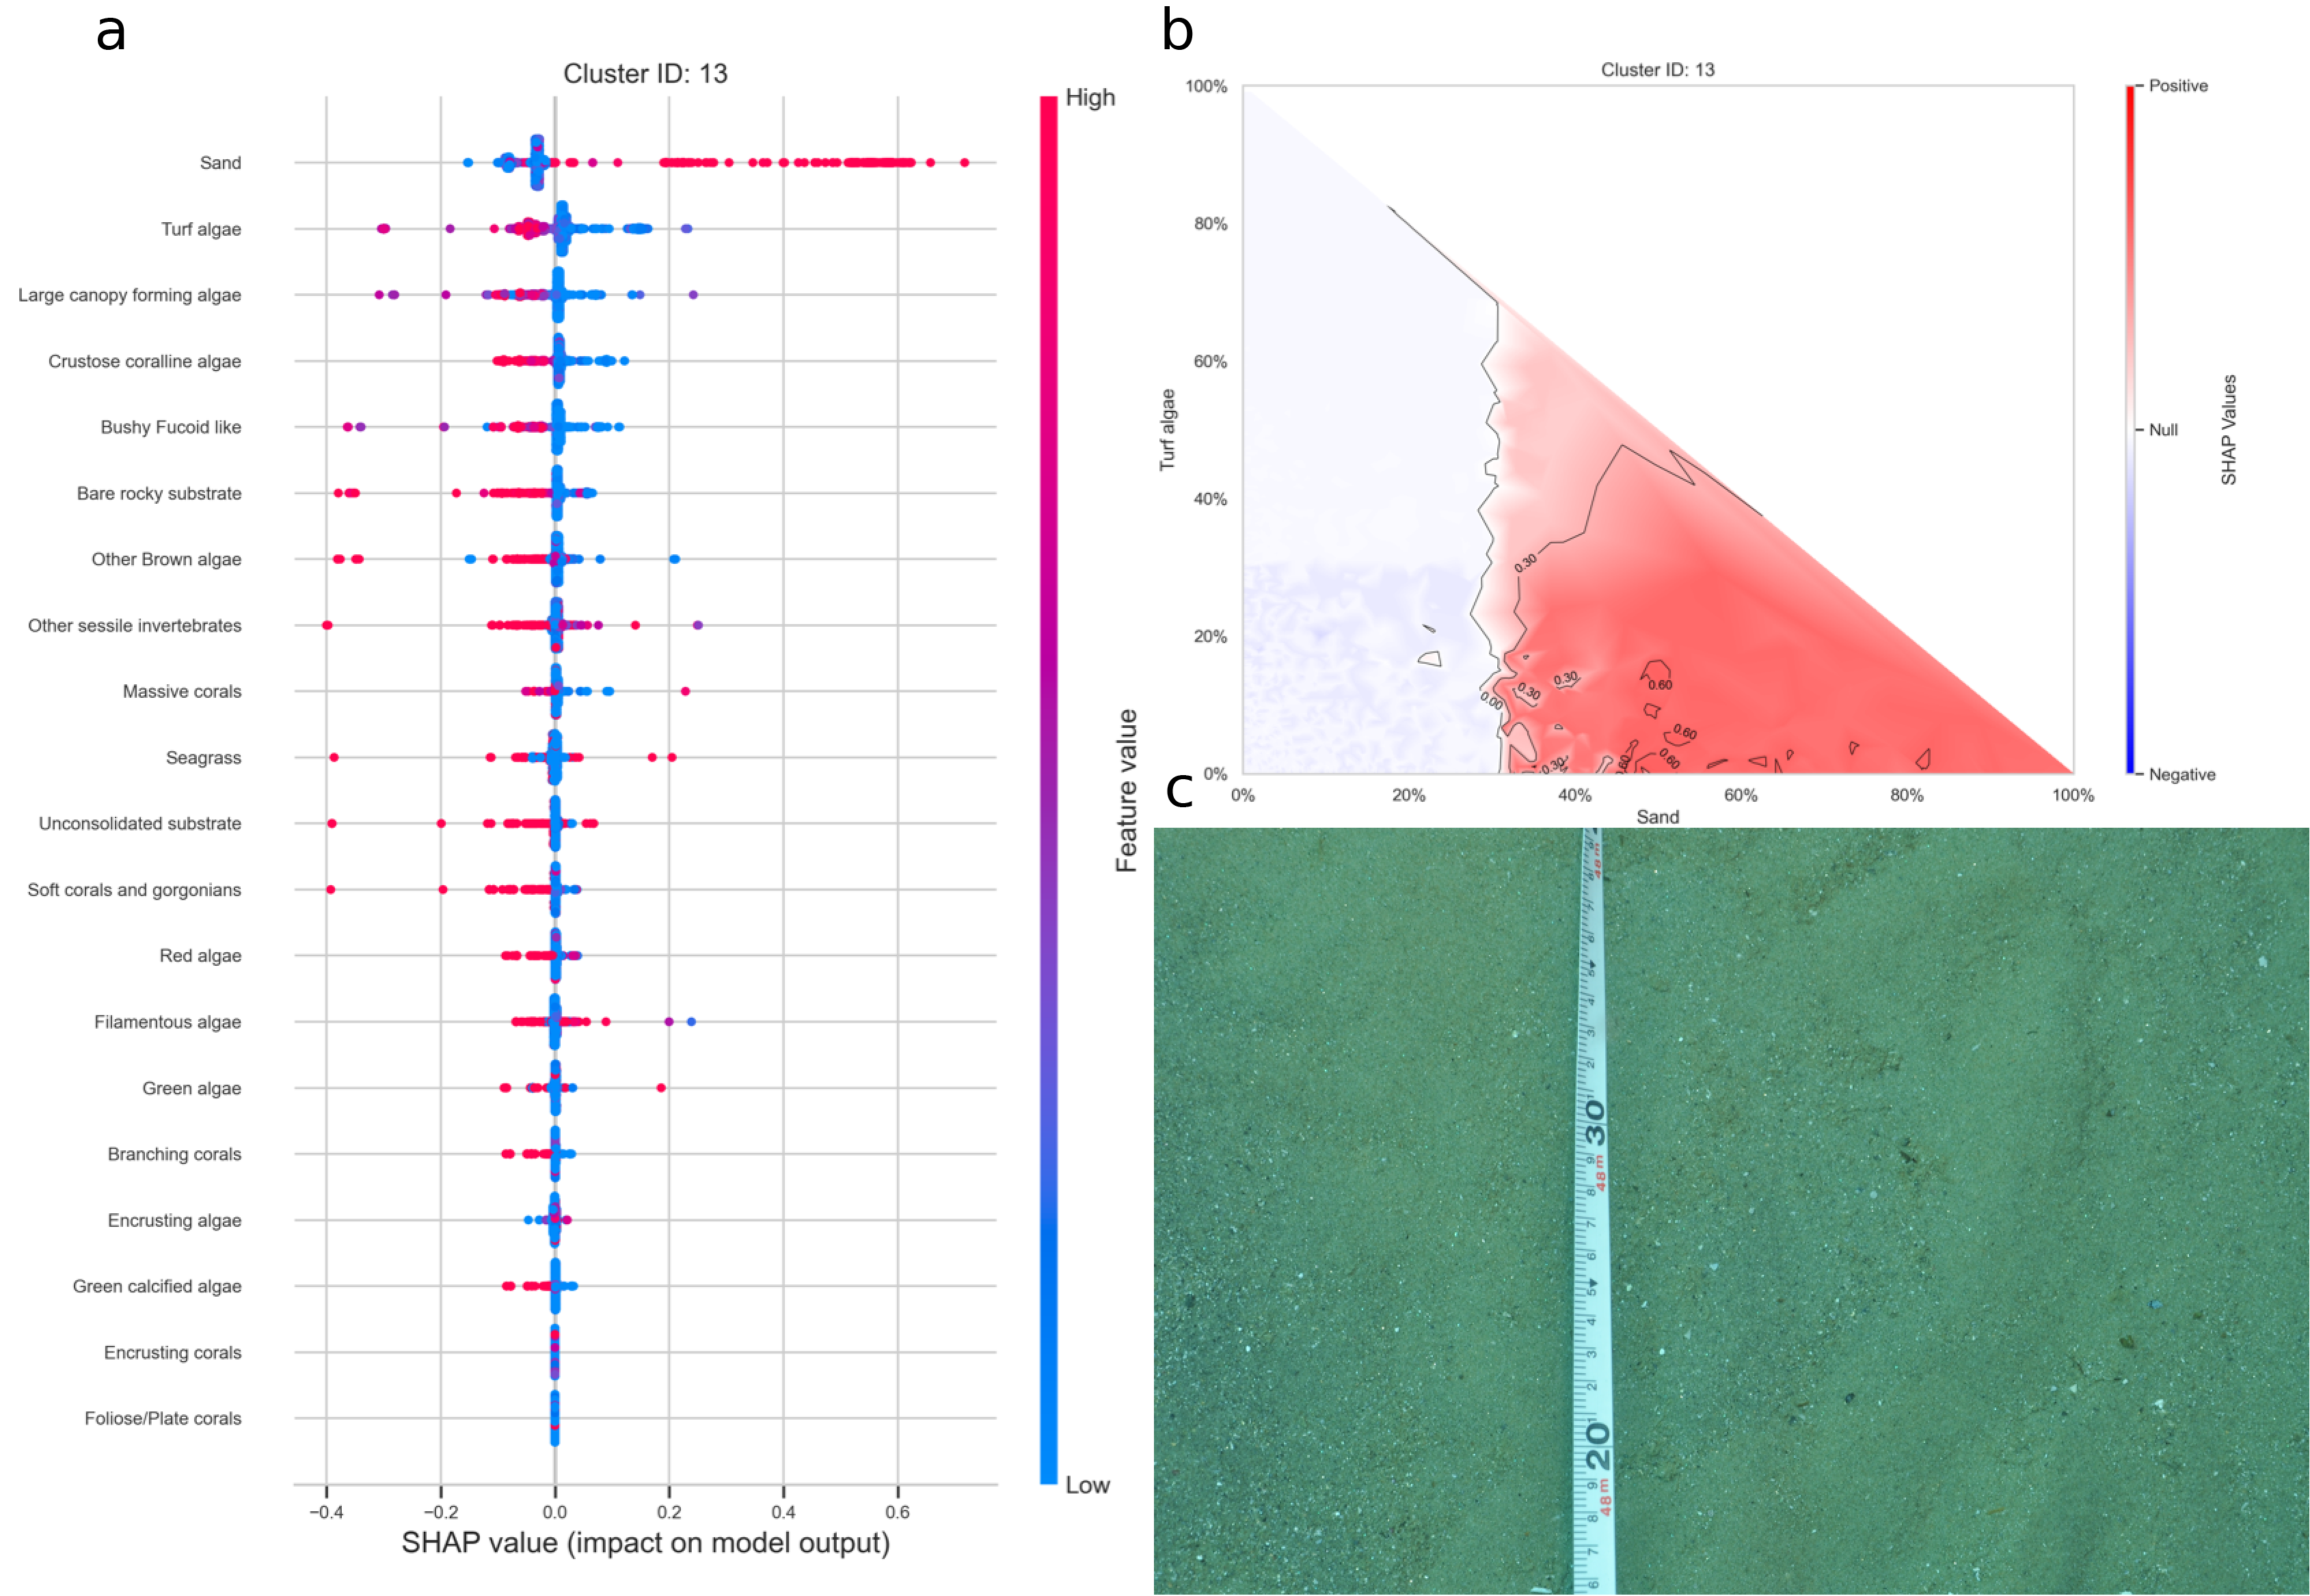
\includegraphics{03-Chapitre2/figures/supplementary/05-explanation_shap_pq_cluster_13.png}
\caption{a. \emph{SHAP} summary plot showing the impact of each habitat
substrate on the classification. The position of each habitat group on
the y-axis indicates its relative importance for the considered cluster.
The position of each point along the x-axis indicates if the observation
is associated with a lower or higher affinity with the cluster and the
colour of the point indicates if the value of the cover of this habitat
is rather high or low. b. Linear interpolation of the \emph{SHAP} values
for the two most influential variables for the cluster \emph{sand}.
c.~Example of photoquadrat for one transect of the cluster \emph{sand}
categorised by \emph{HDBSCAN} as exemplary.}\label{fig:chap2figS33}
}
\end{figure}

\begin{figure}
\hypertarget{fig:chap2figS34}{%
\centering
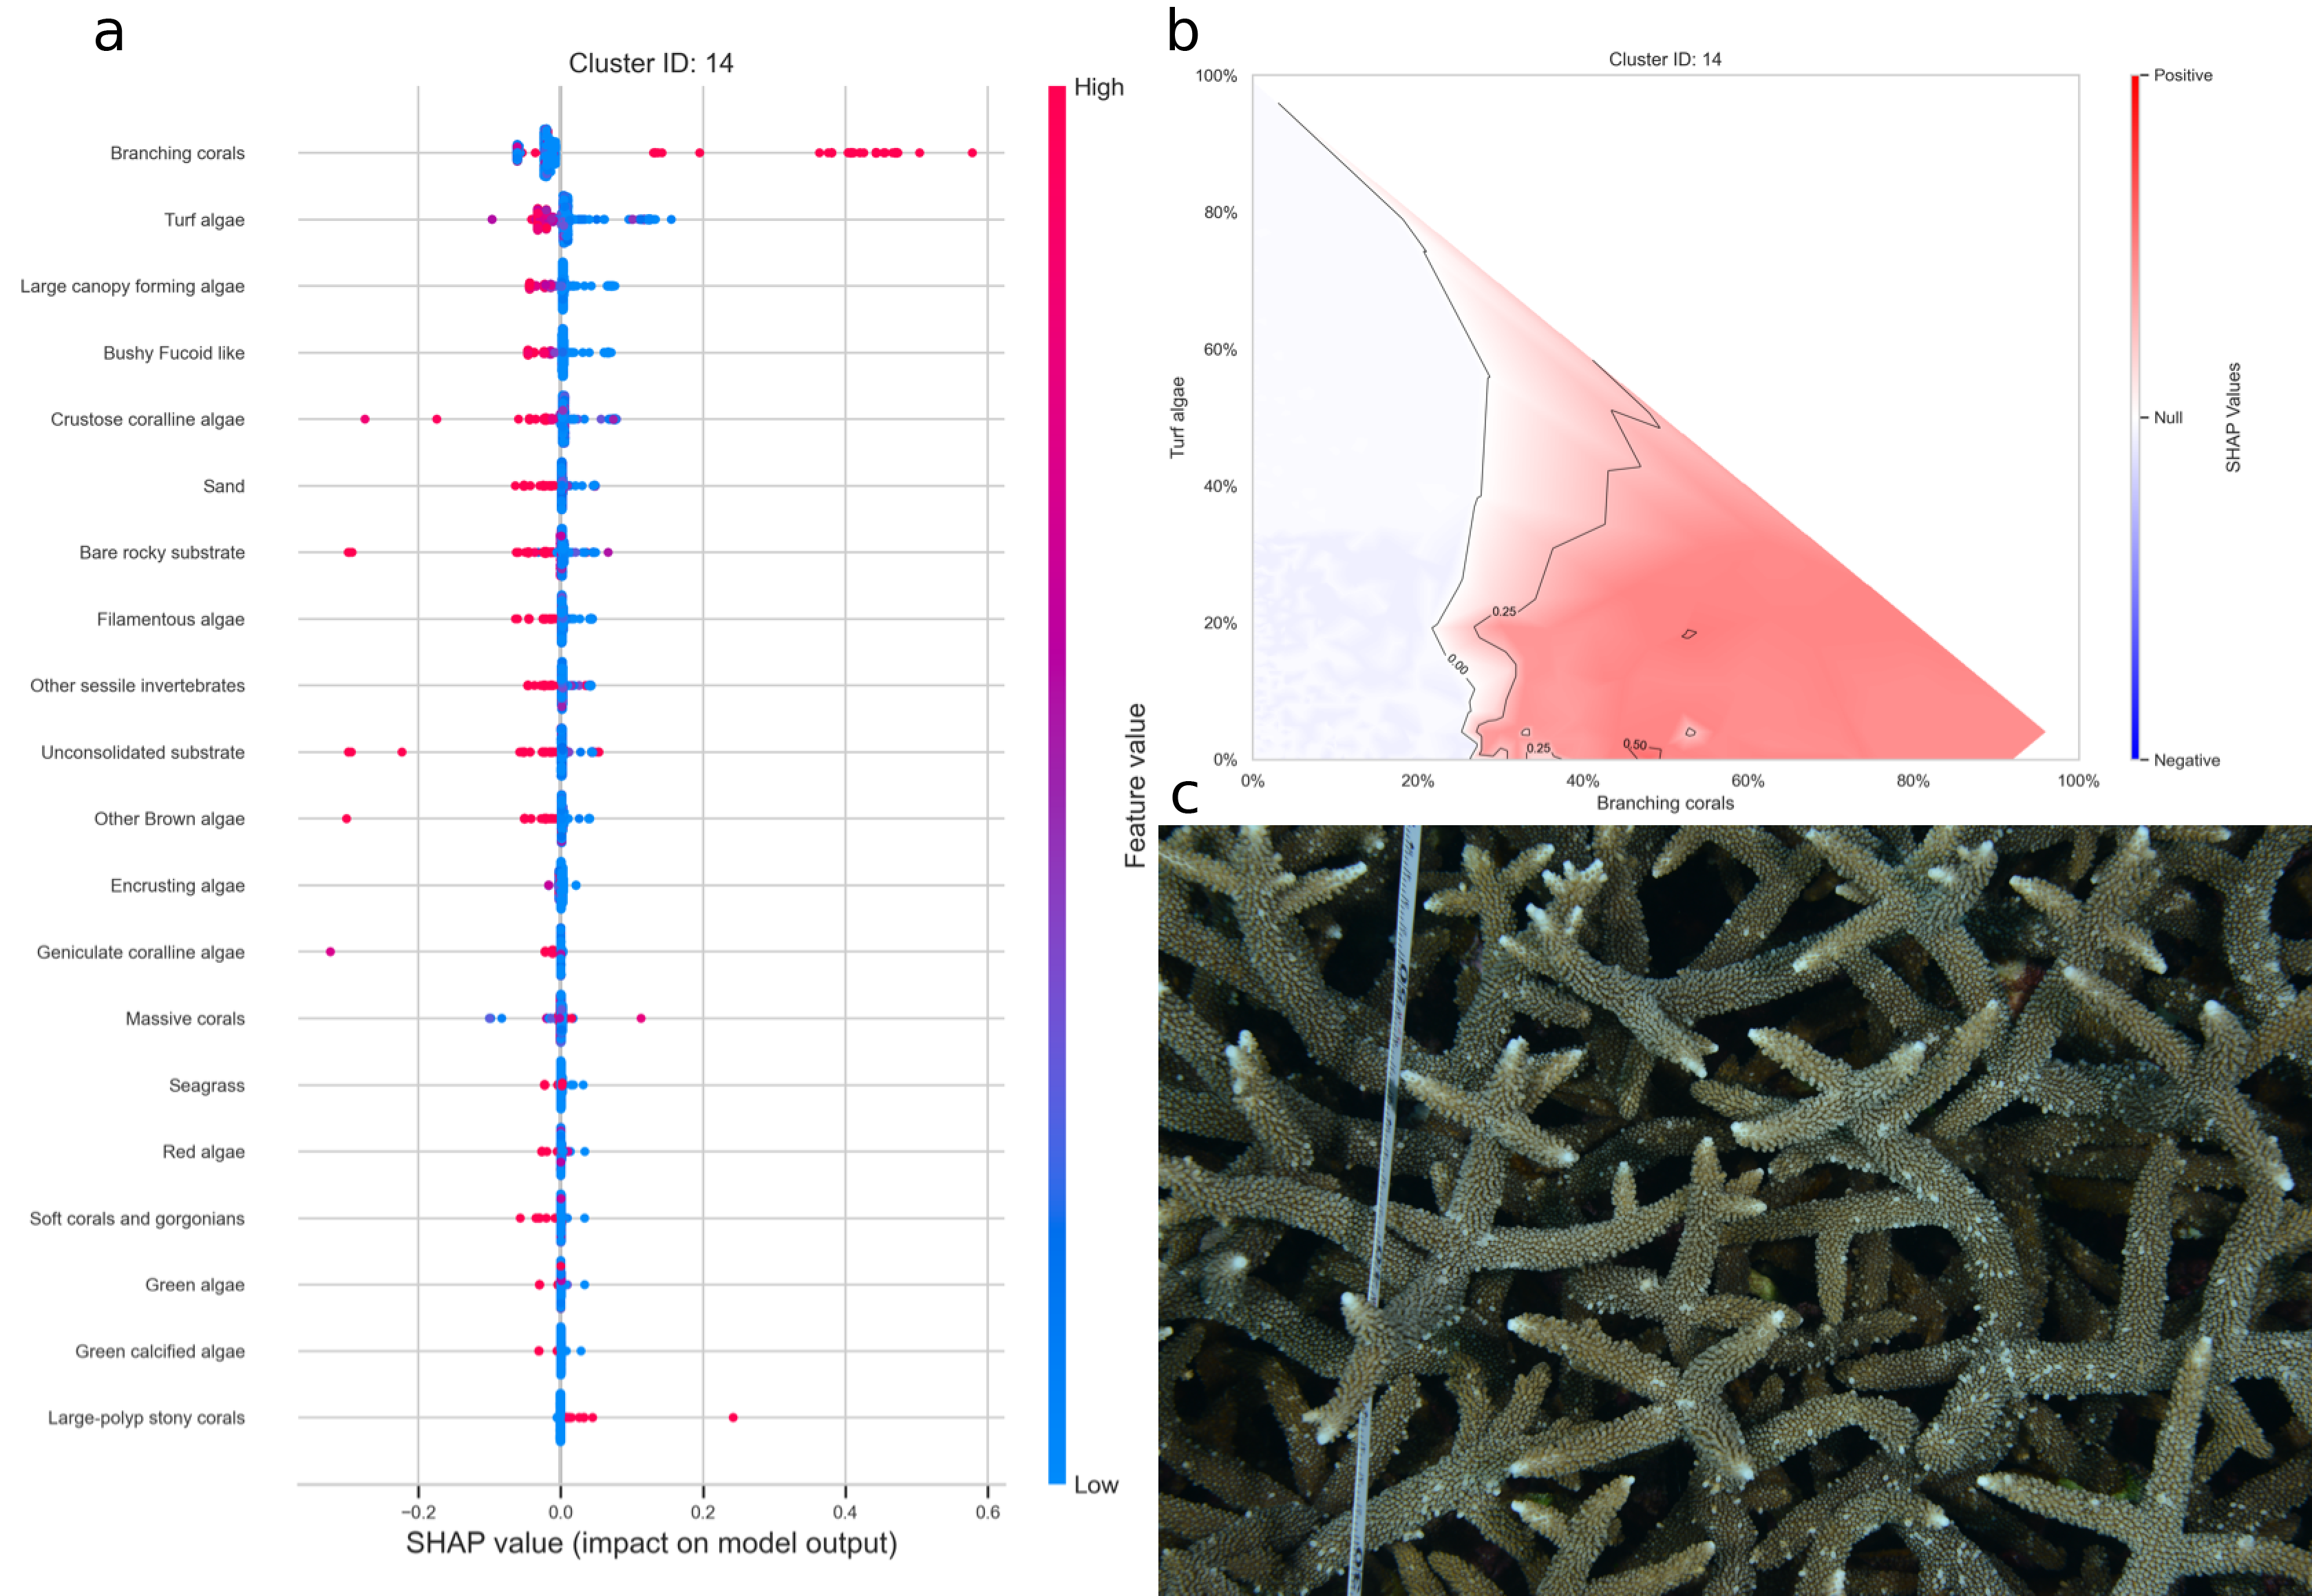
\includegraphics{03-Chapitre2/figures/supplementary/05-explanation_shap_pq_cluster_14.png}
\caption{a. \emph{SHAP} summary plot showing the impact of each habitat
substrate on the classification. The position of each habitat group on
the y-axis indicates its relative importance for the considered cluster.
The position of each point along the x-axis indicates if the observation
is associated with a lower or higher affinity with the cluster and the
colour of the point indicates if the value of the cover of this habitat
is rather high or low. b. Linear interpolation of the \emph{SHAP} values
for the two most influential variables for the cluster \emph{branching
coral}. c.~Example of photoquadrat for one transect of the cluster
\emph{branching coral} categorised by \emph{HDBSCAN} as
exemplary.}\label{fig:chap2figS34}
}
\end{figure}

\begin{figure}
\hypertarget{fig:chap2figS35}{%
\centering
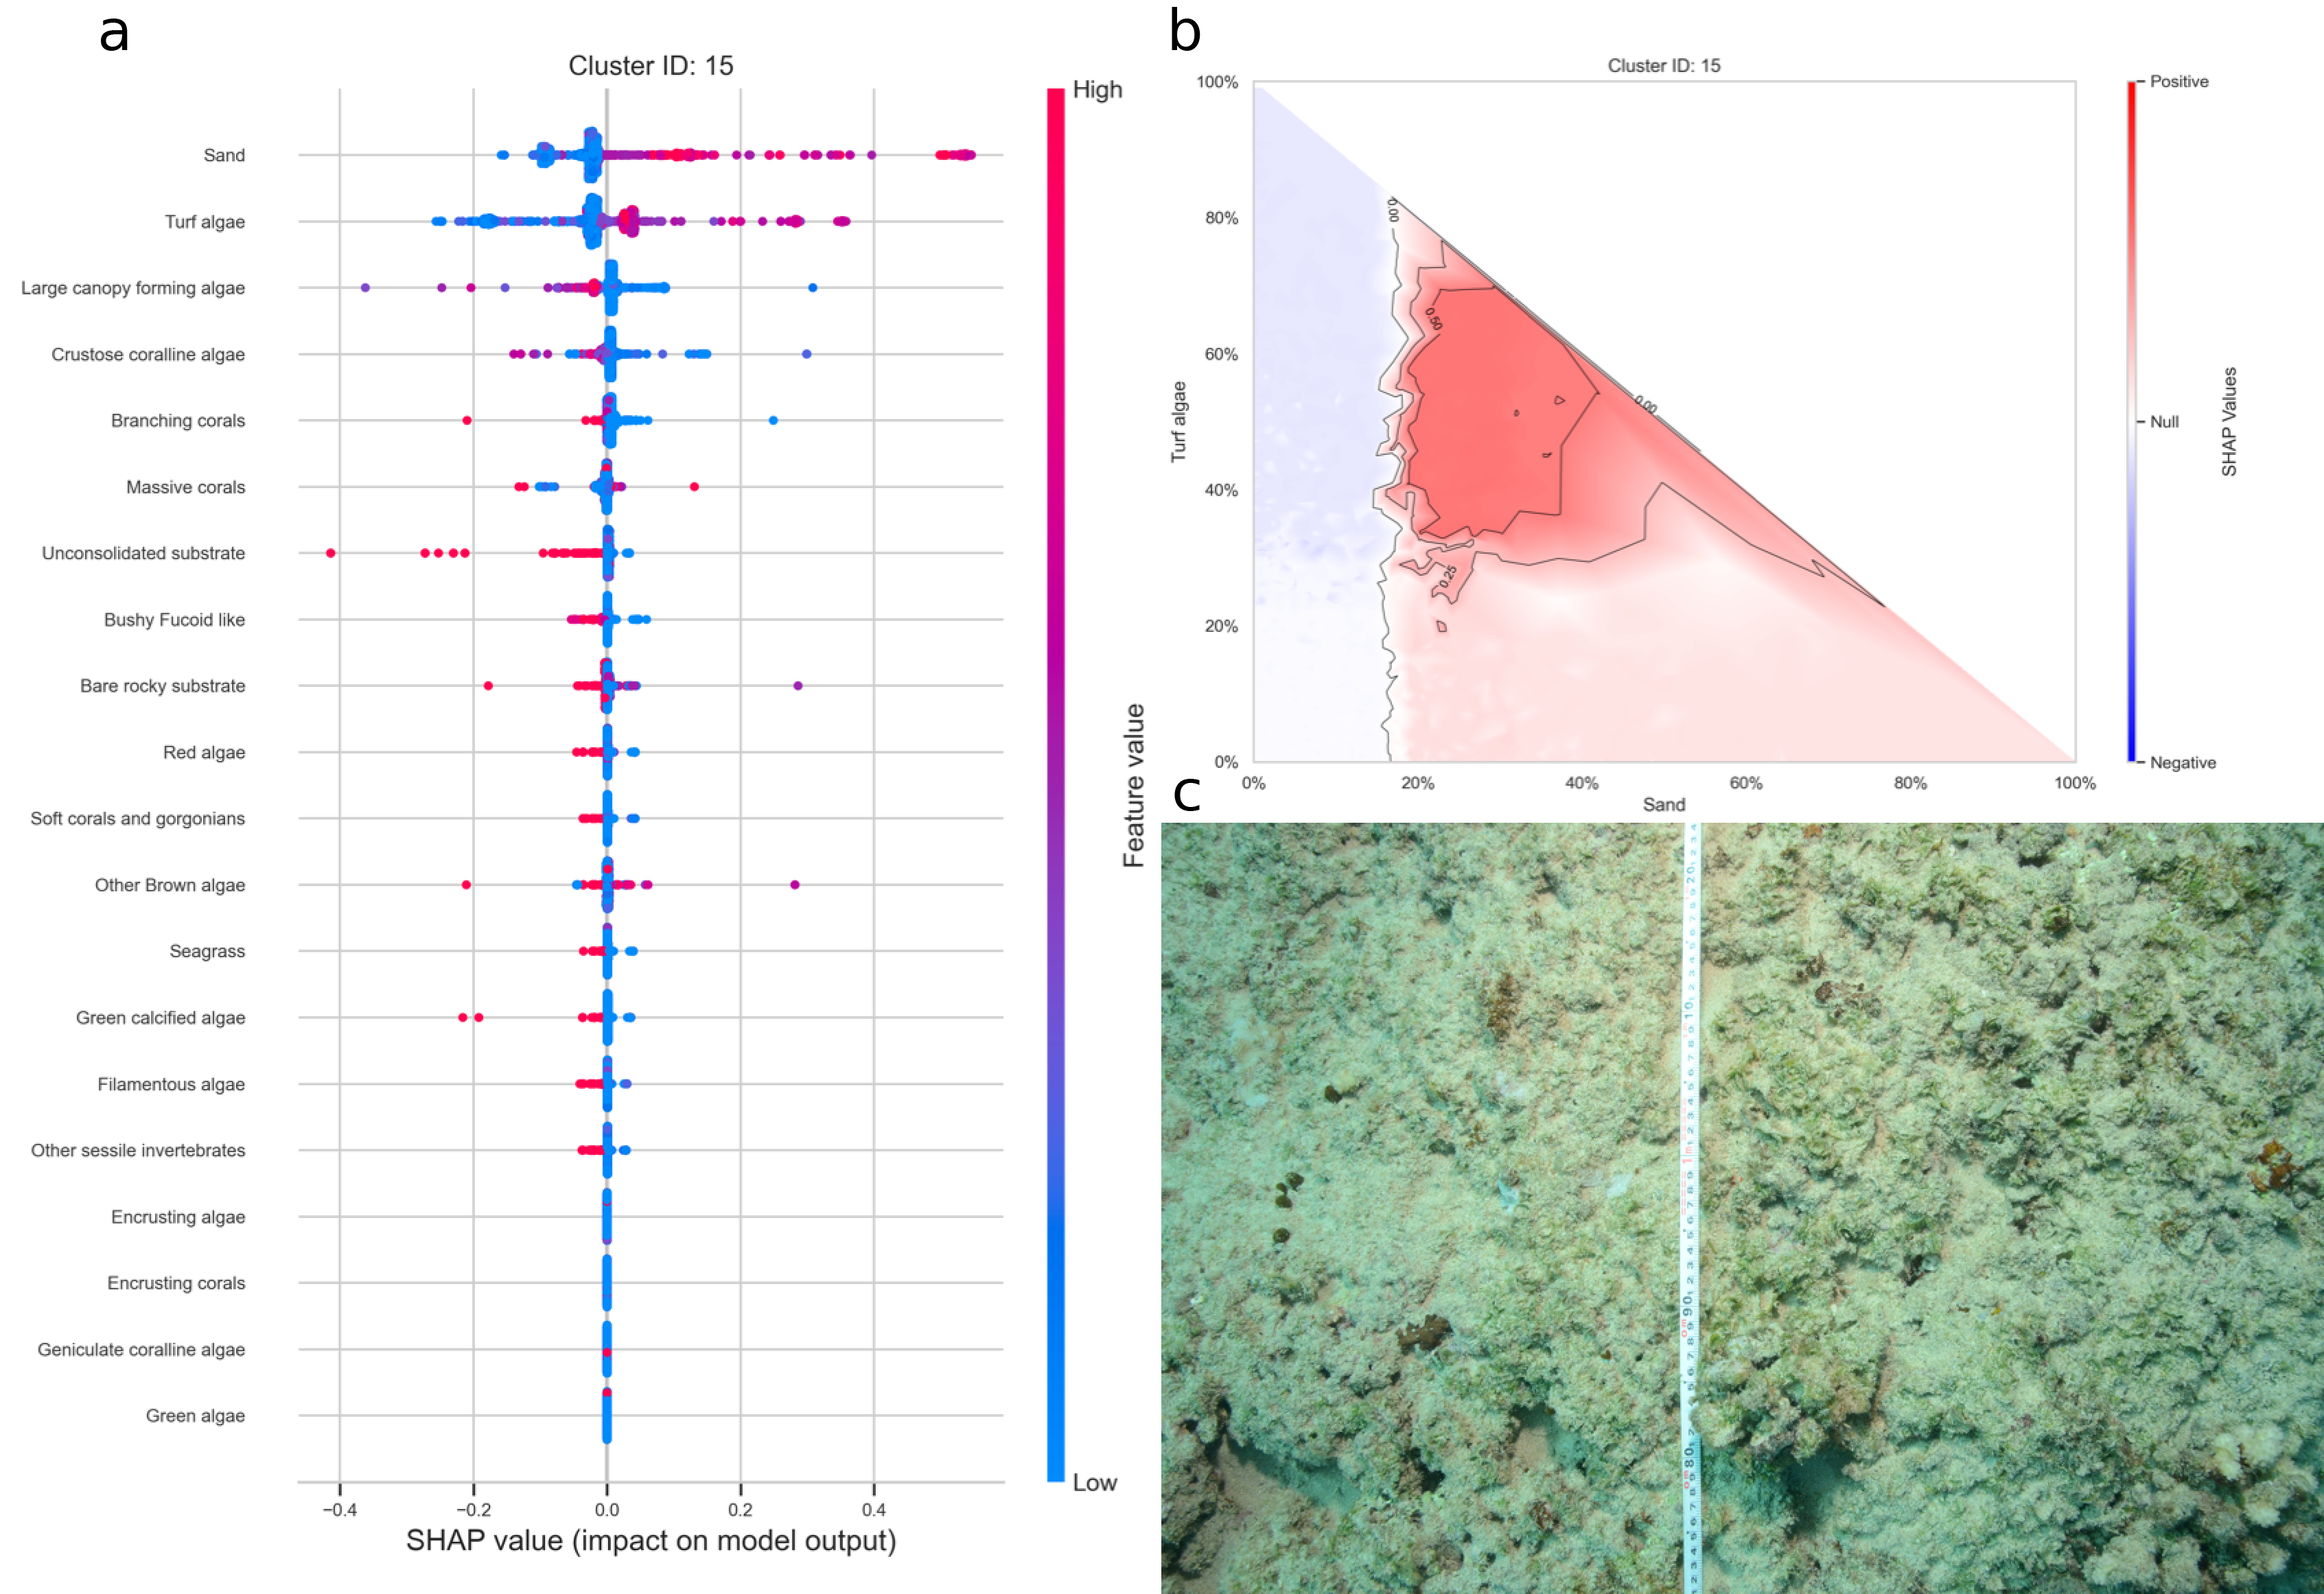
\includegraphics{03-Chapitre2/figures/supplementary/05-explanation_shap_pq_cluster_15.png}
\caption{a. \emph{SHAP} summary plot showing the impact of each habitat
substrate on the classification. The position of each habitat group on
the y-axis indicates its relative importance for the considered cluster.
The position of each point along the x-axis indicates if the observation
is associated with a lower or higher affinity with the cluster and the
colour of the point indicates if the value of the cover of this habitat
is rather high or low. b. Linear interpolation of the \emph{SHAP} values
for the two most influential variables for the cluster \emph{sand and
turf algae}. c.~Example of photoquadrat for one transect of the cluster
\emph{sand and turf algae} categorised by \emph{HDBSCAN} as
exemplary.}\label{fig:chap2figS35}
}
\end{figure}

\begin{figure}
\hypertarget{fig:chap2figS36}{%
\centering
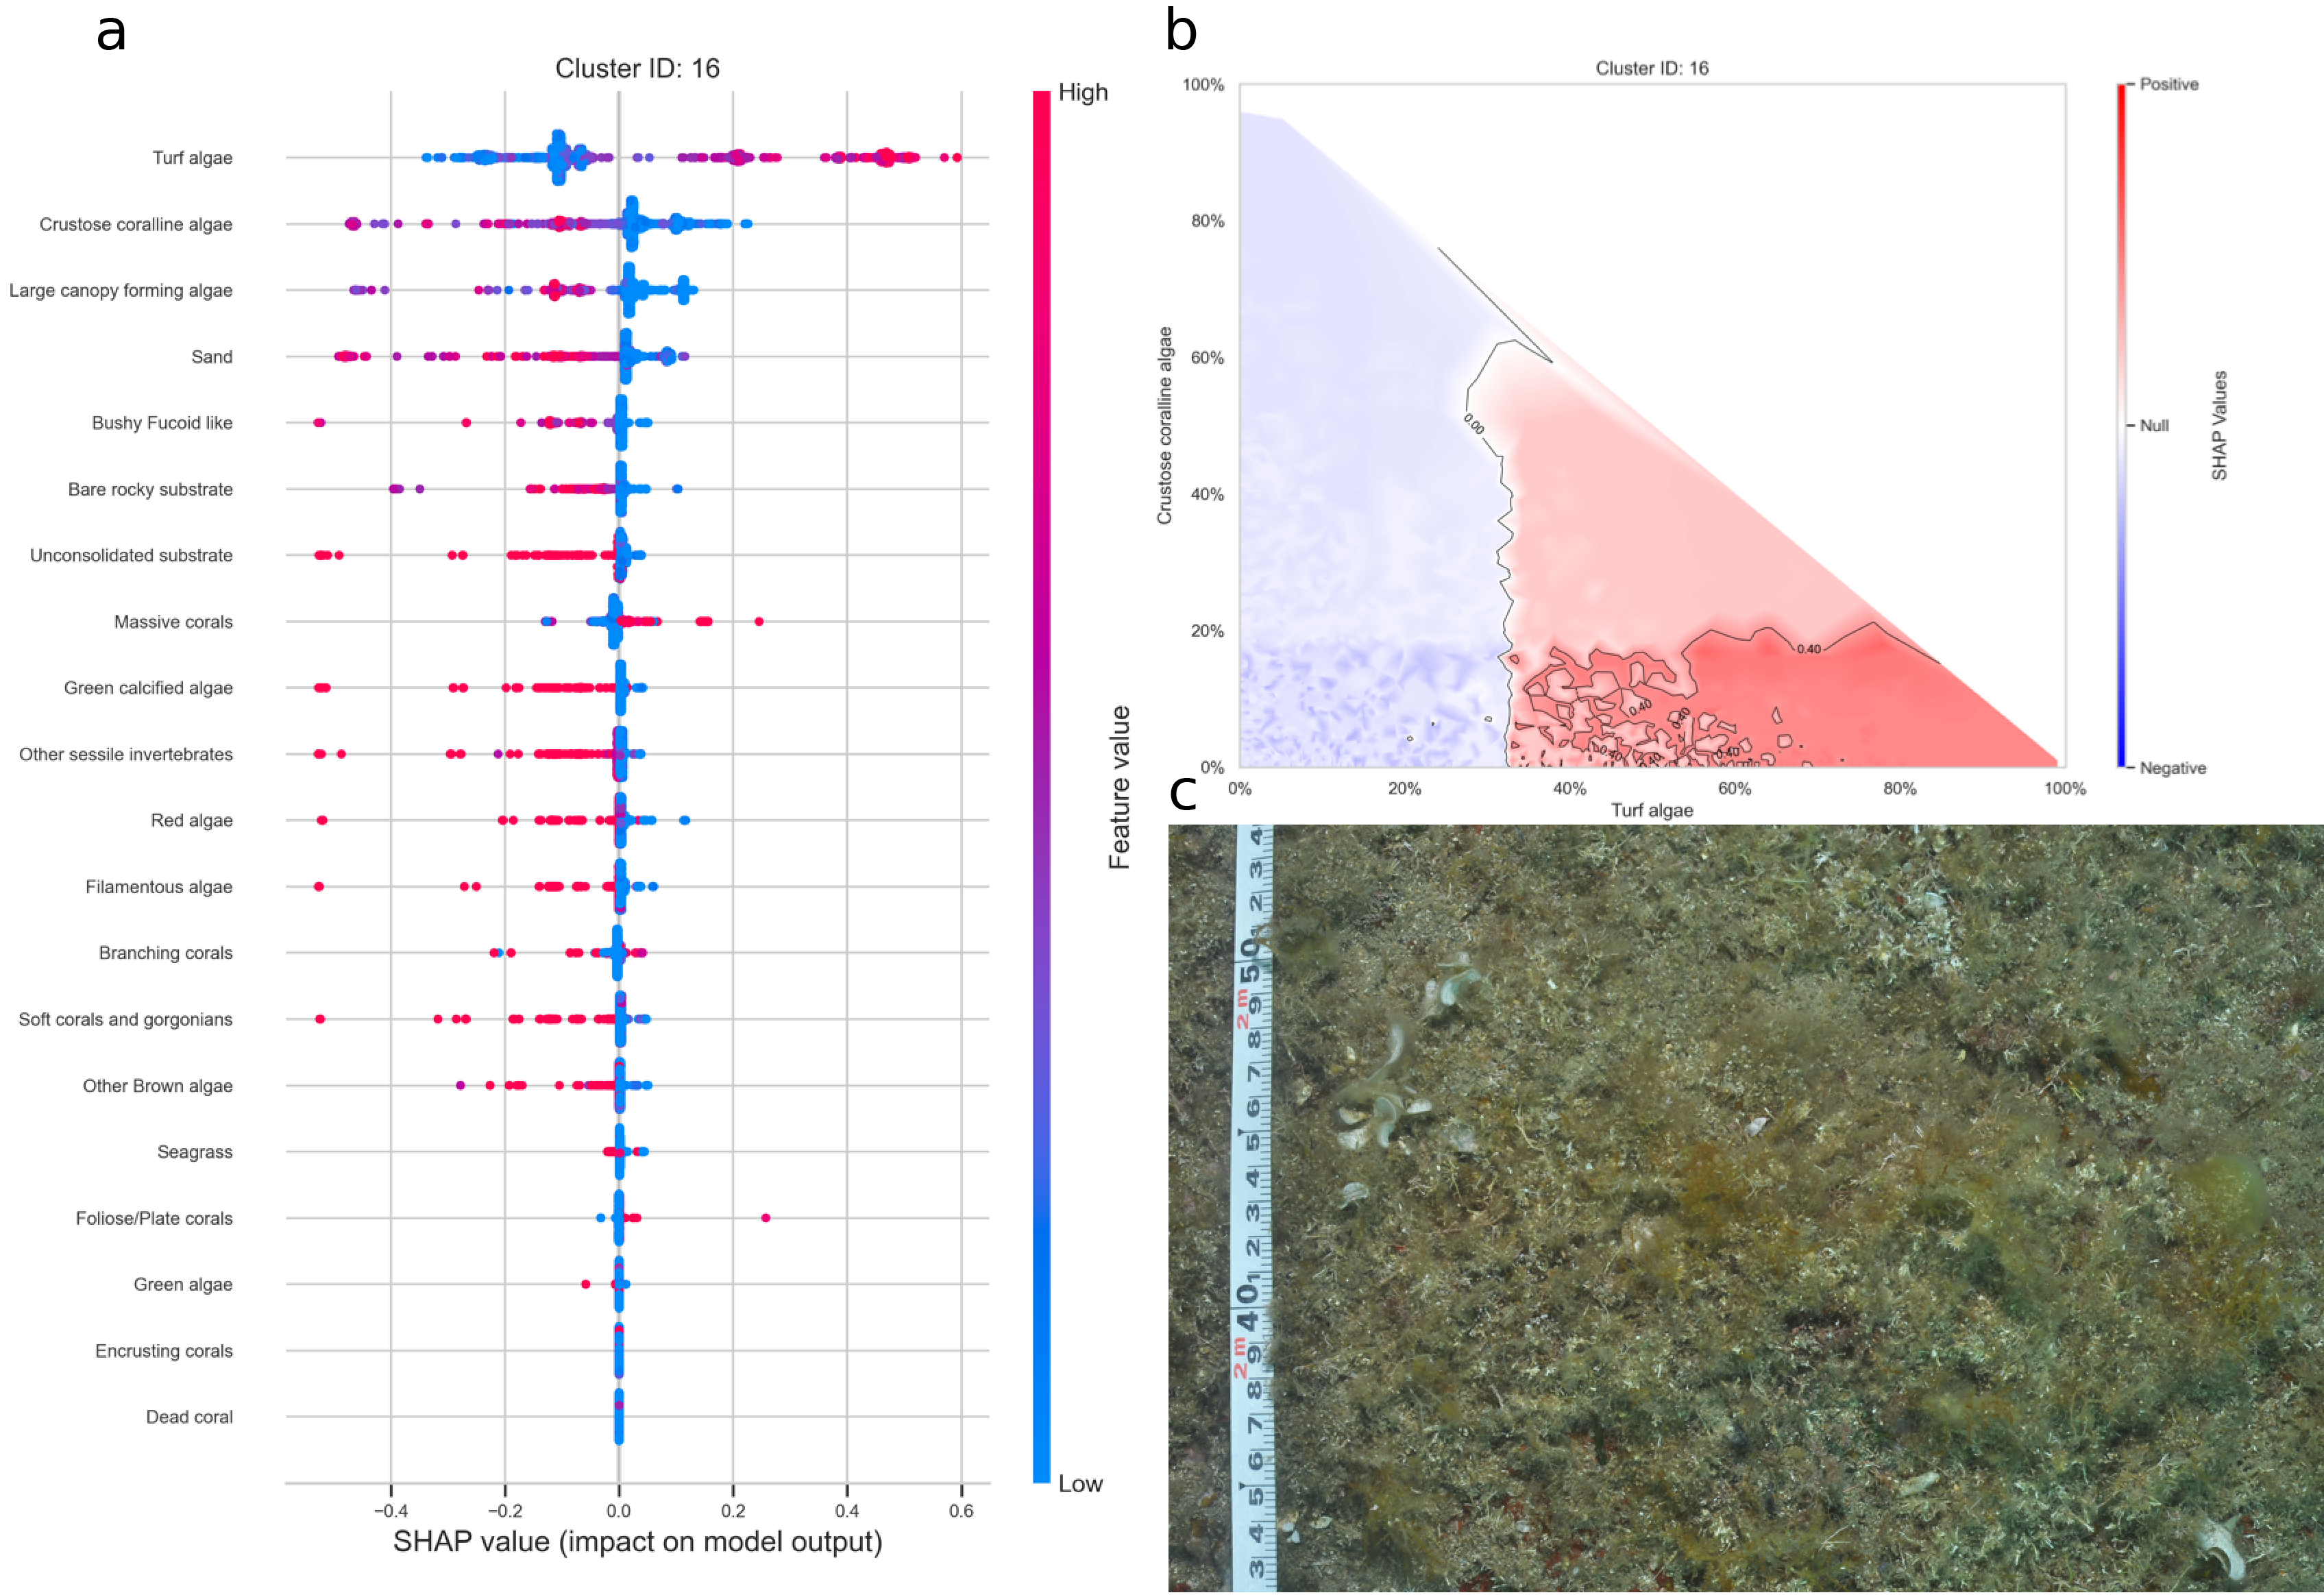
\includegraphics{03-Chapitre2/figures/supplementary/05-explanation_shap_pq_cluster_16.png}
\caption{a. \emph{SHAP} summary plot showing the impact of each habitat
substrate on the classification. The position of each habitat group on
the y-axis indicates its relative importance for the considered cluster.
The position of each point along the x-axis indicates if the observation
is associated with a lower or higher affinity with the cluster and the
colour of the point indicates if the value of the cover of this habitat
is rather high or low. b. Linear interpolation of the \emph{SHAP} values
for the two most influential variables for the cluster \emph{turf
algae}. c.~Example of photoquadrat for one transect of the cluster
\emph{turf algae} categorised by \emph{HDBSCAN} as
exemplary.}\label{fig:chap2figS36}
}
\end{figure}

\clearpage

\hypertarget{appendixD-chapter2}{%
\section*{Appendix D - Complementary results}\label{appendixD-chapter2}}
\addcontentsline{toc}{section}{Appendix D - Complementary results}

\begin{figure}
\hypertarget{fig:chap2figS37}{%
\centering
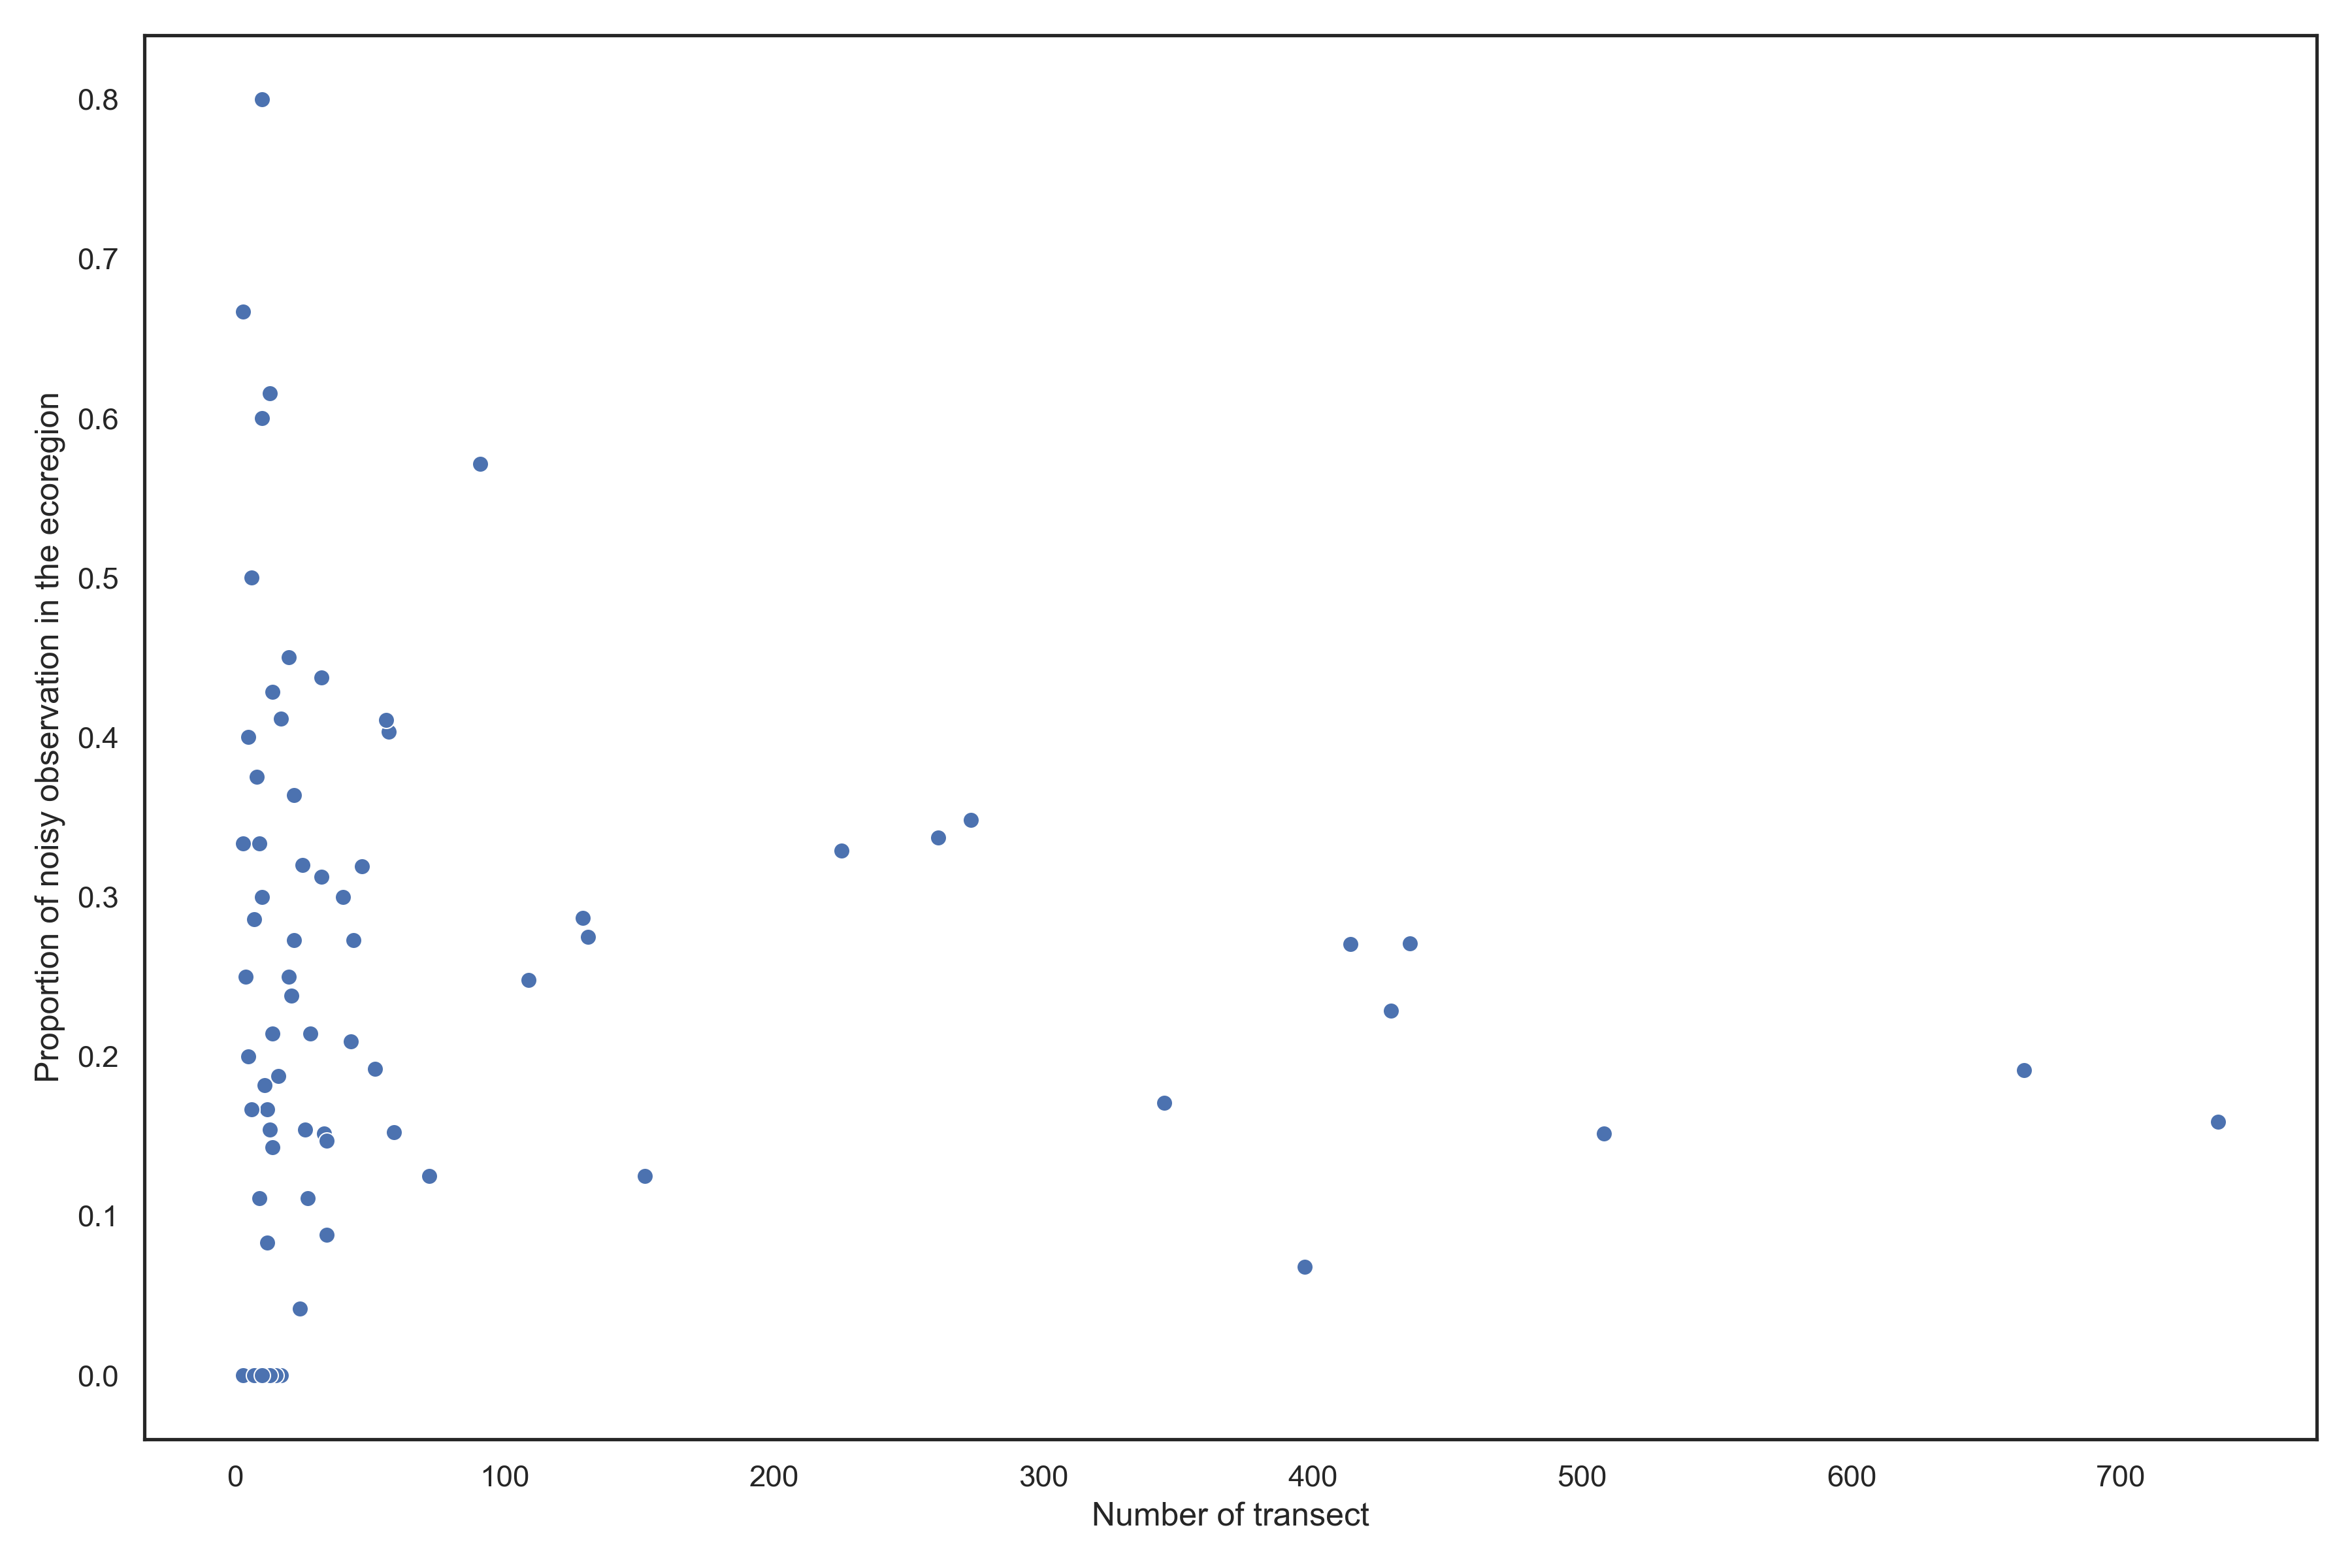
\includegraphics{03-Chapitre2/figures/supplementary/07-prop_noisy_nb_obs.png}
\caption{Plot of the proportion of transect classified as noisy by the
\emph{UMAP-HDBSCAN} pipeline as a function of the log10(number of
transects) sampled within an ecoregion}\label{fig:chap2figS37}
}
\end{figure}

\begin{figure}
\hypertarget{fig:chap2figS38}{%
\centering
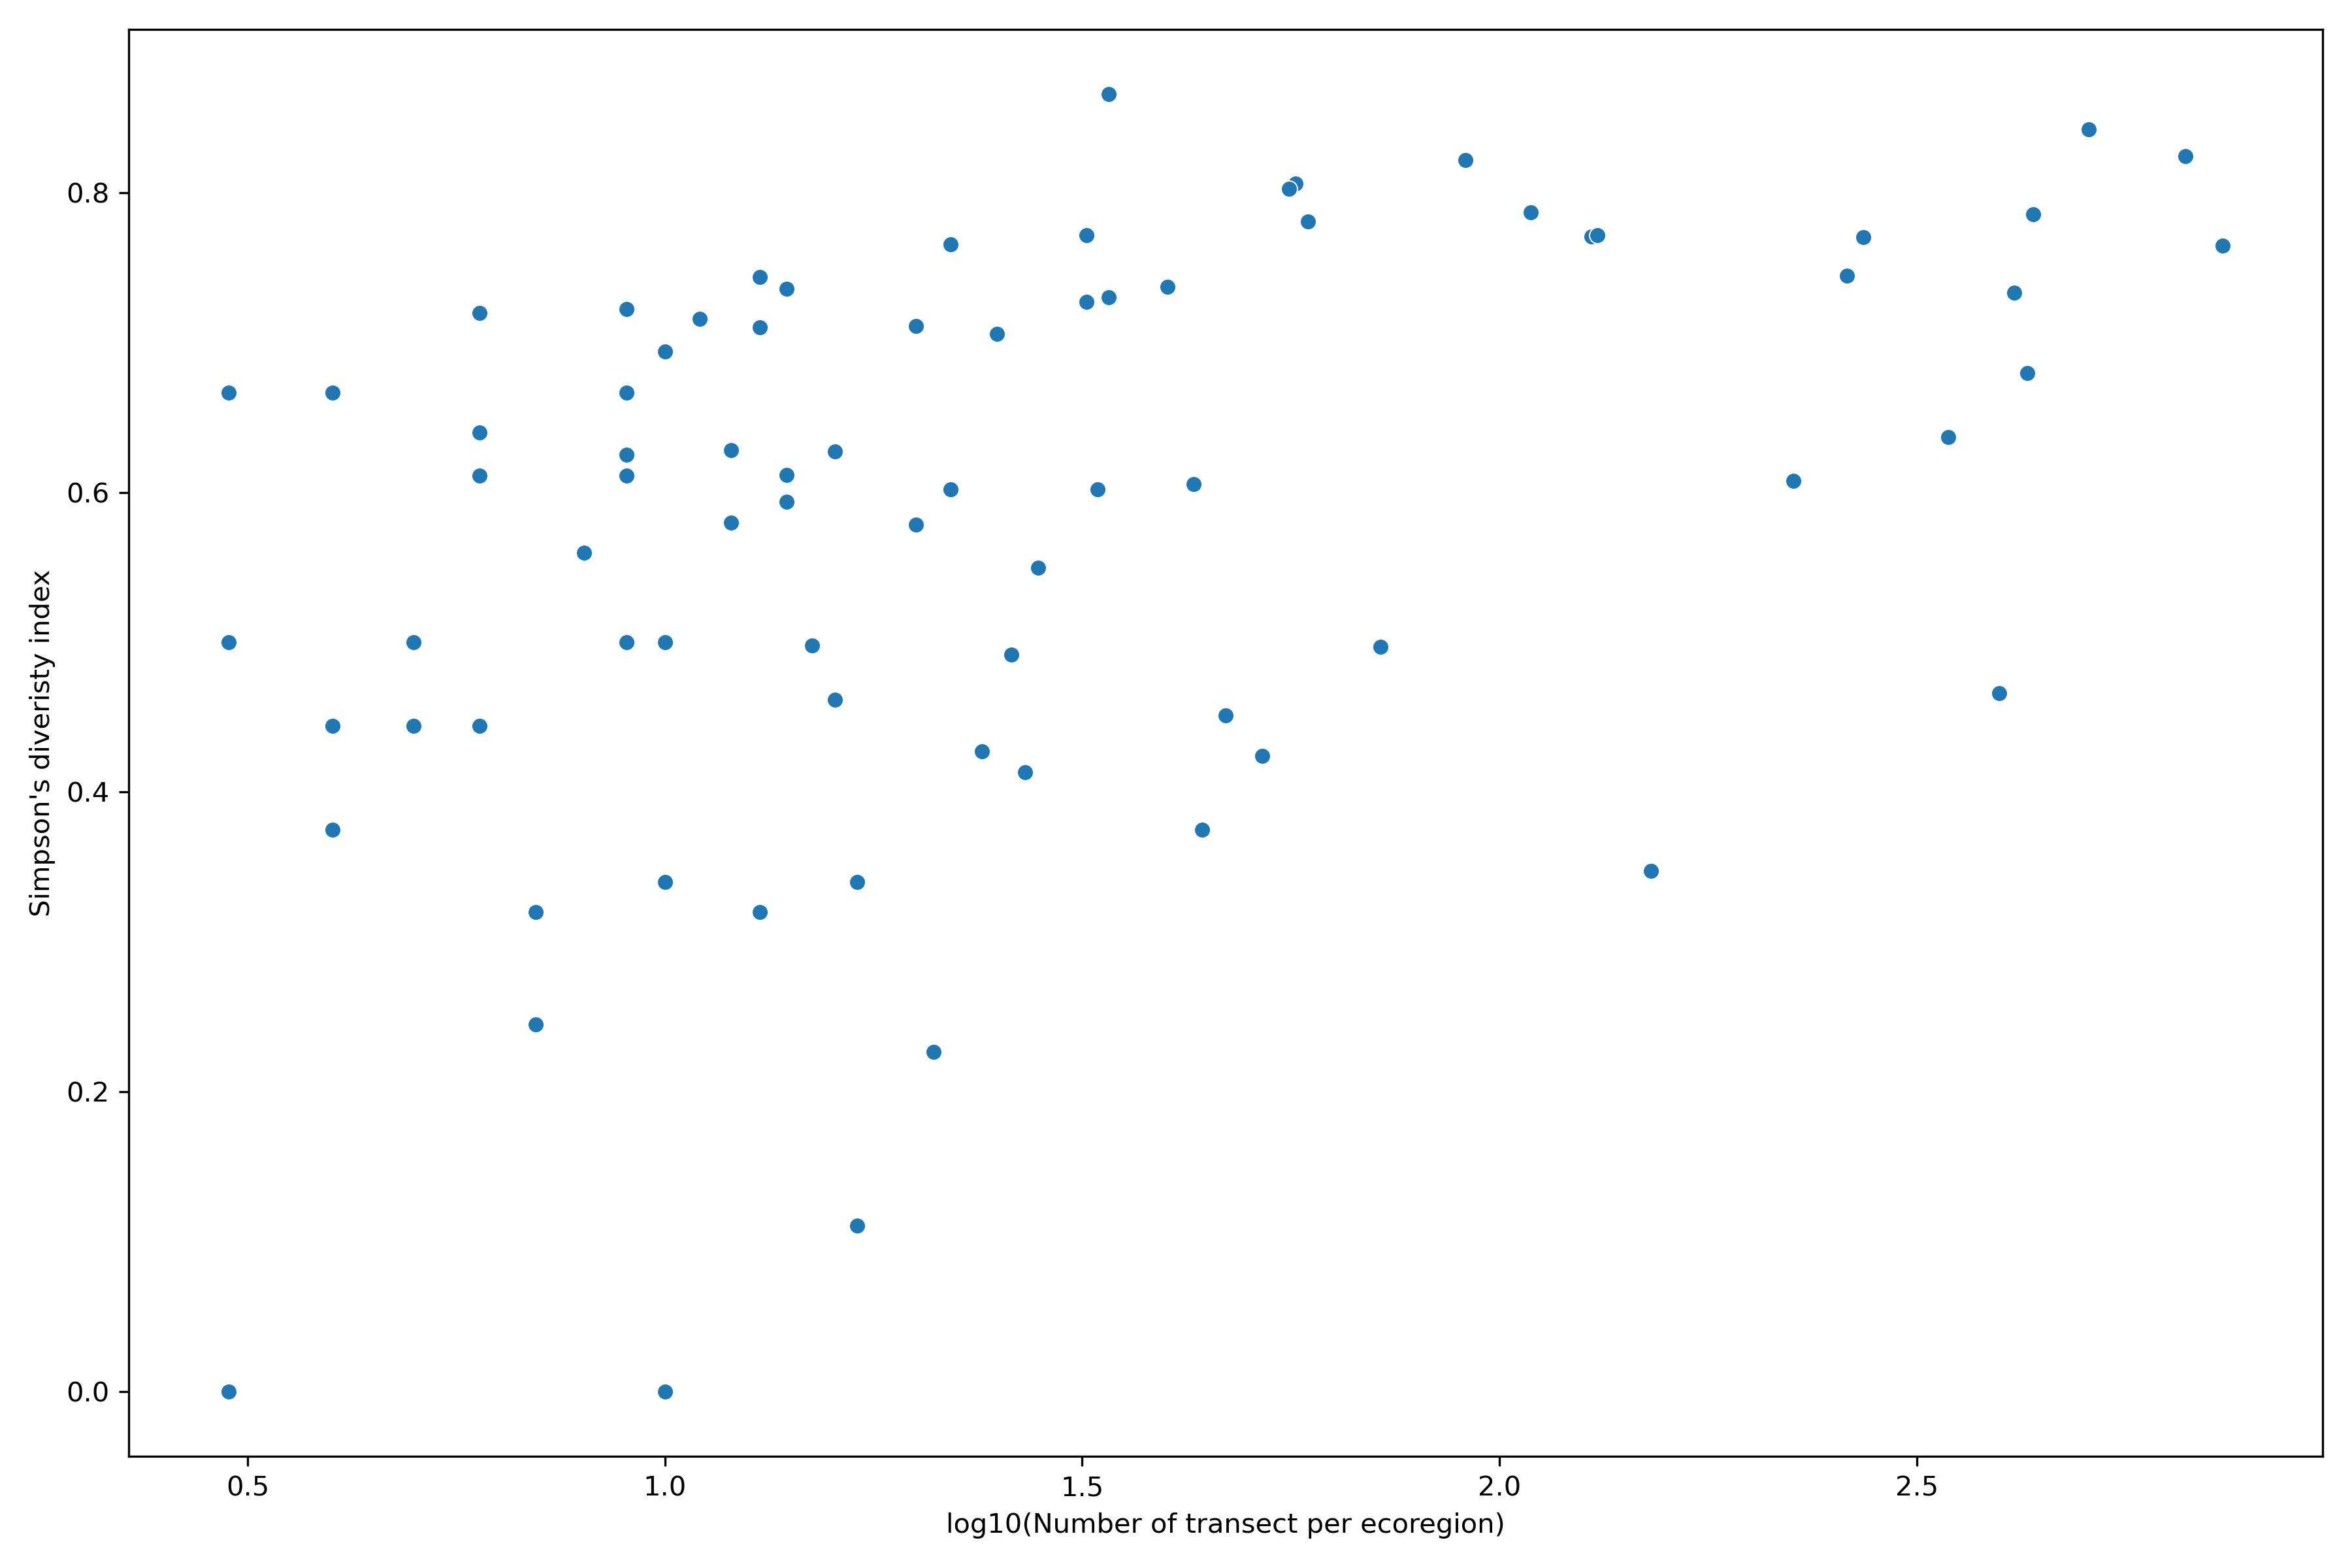
\includegraphics{03-Chapitre2/figures/supplementary/07-simpsons_div_nobs.png}
\caption{Plot of the Gini-Simpson diversity index as a function of the
log10(number of transects) sampled within an
ecoregion}\label{fig:chap2figS38}
}
\end{figure}

\begin{figure}
\hypertarget{fig:chap2figS42}{%
\centering
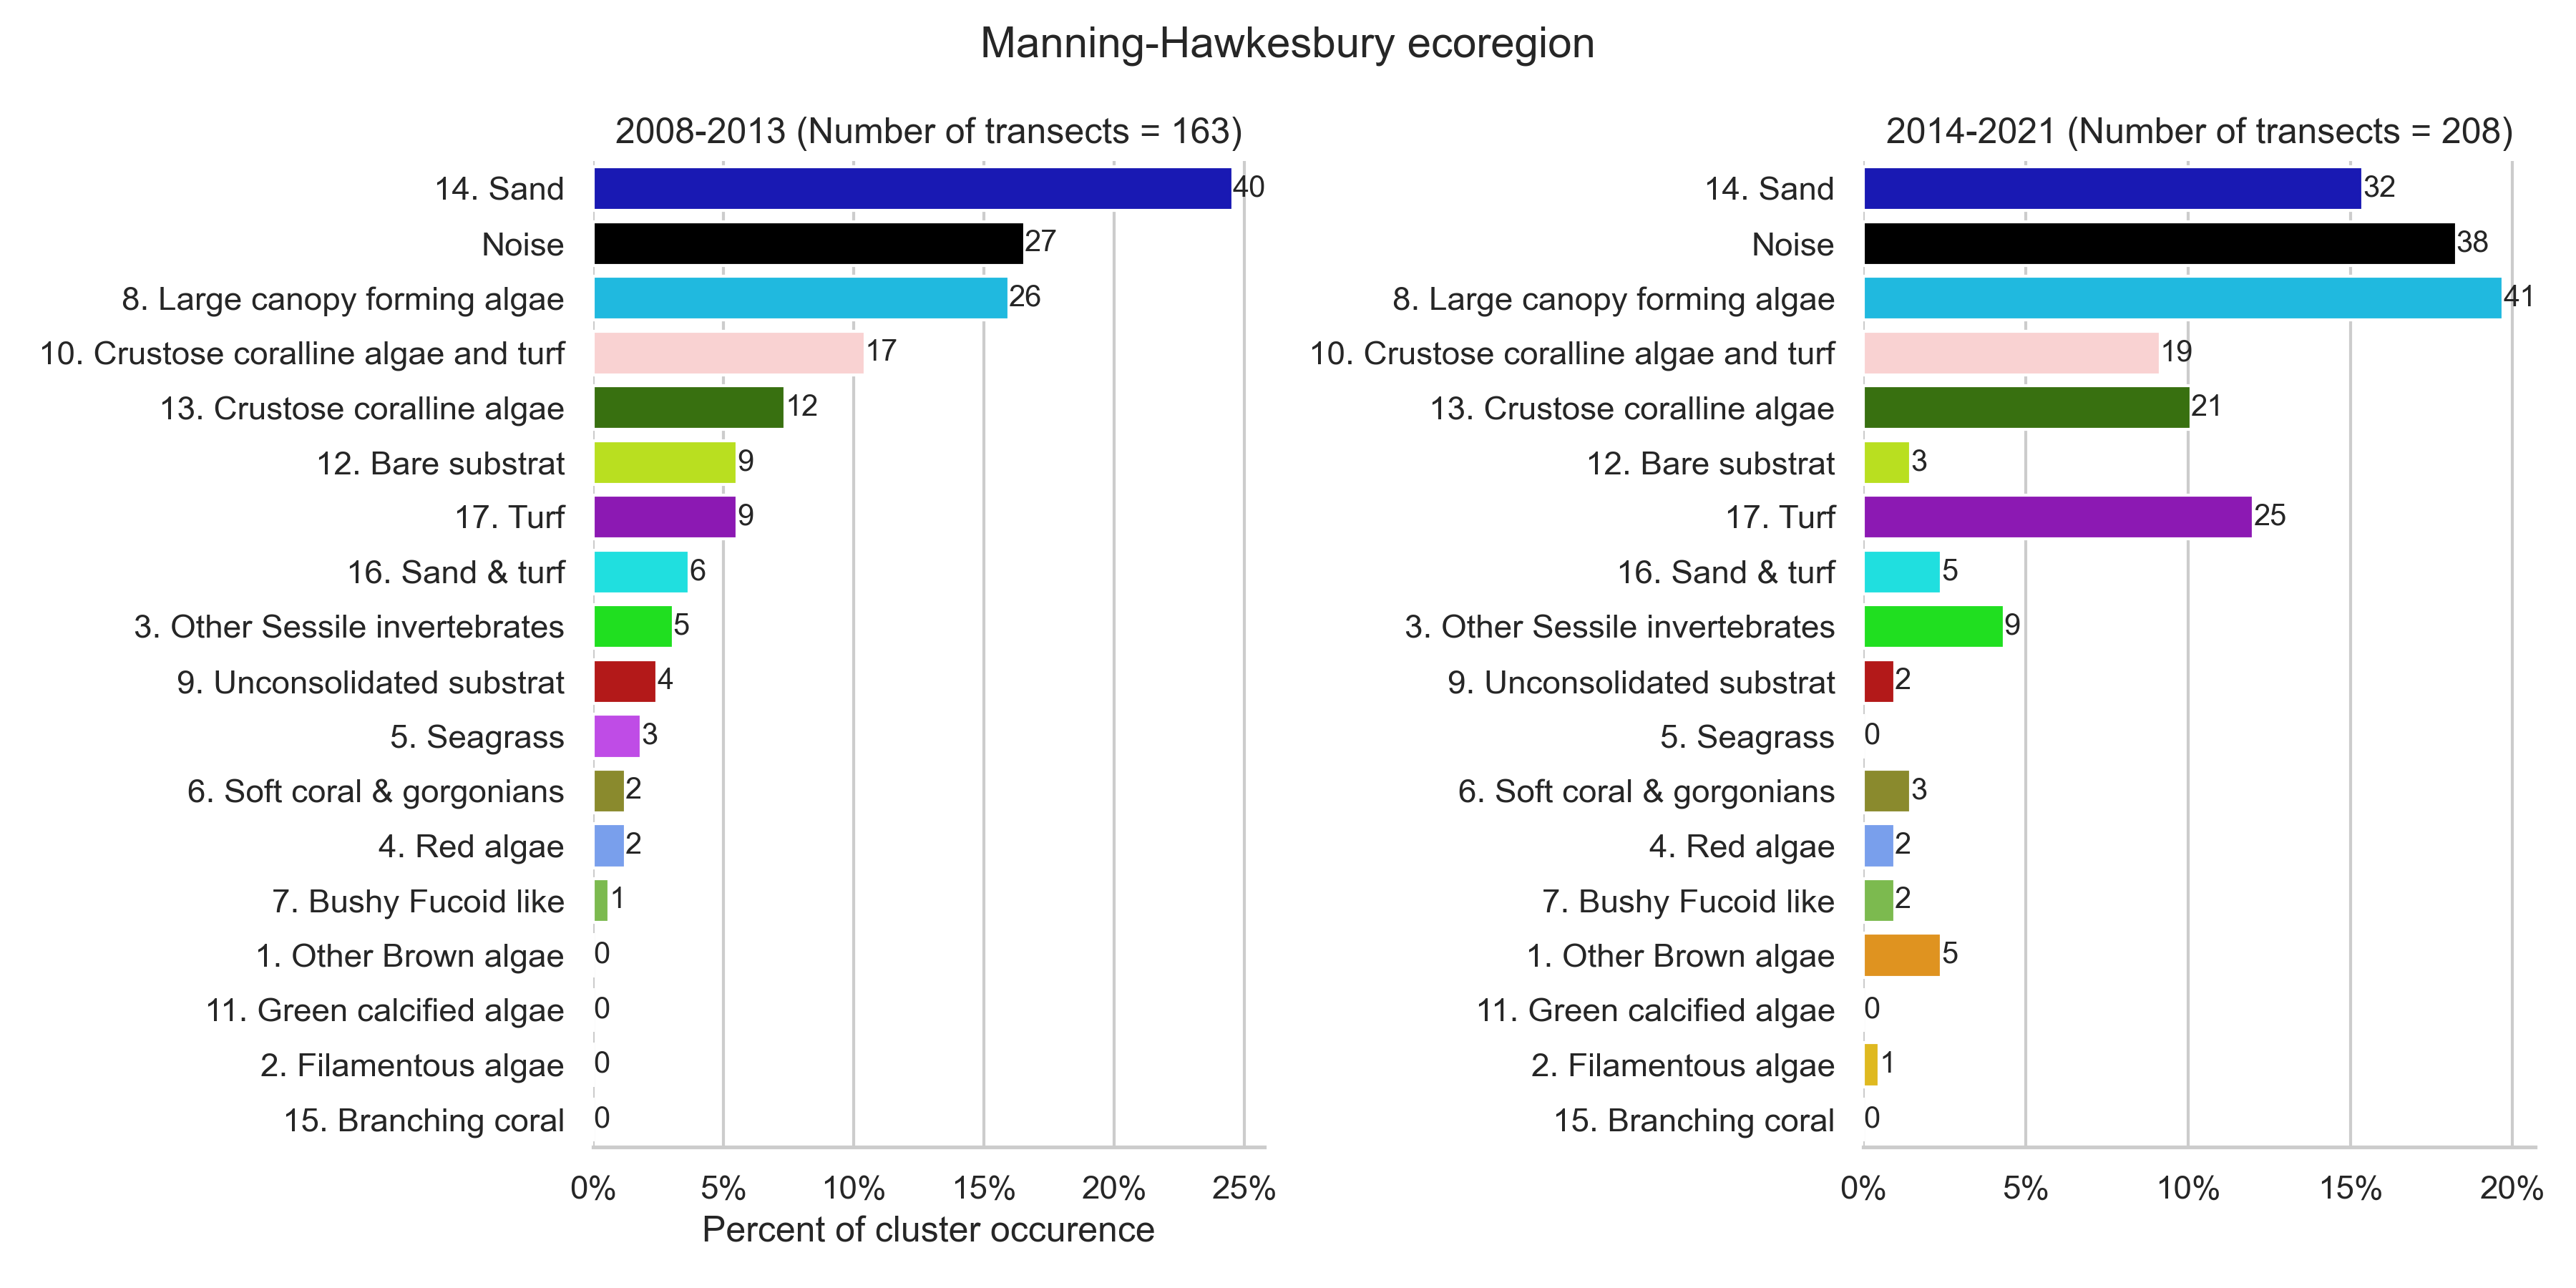
\includegraphics{03-Chapitre2/figures/supplementary/08-temporal_change_ecoregion_Manning-Hawkesbury.png}
\caption{Bar graph of the proportion of different clusters for the
period 2008-2013 and 2015-2021 for sites that were sampled at least once
in each of the two periods for the Manning-Hawkesbury
ecoregion.}\label{fig:chap2figS42}
}
\end{figure}

\begin{figure}
\hypertarget{fig:chap2figS40}{%
\centering
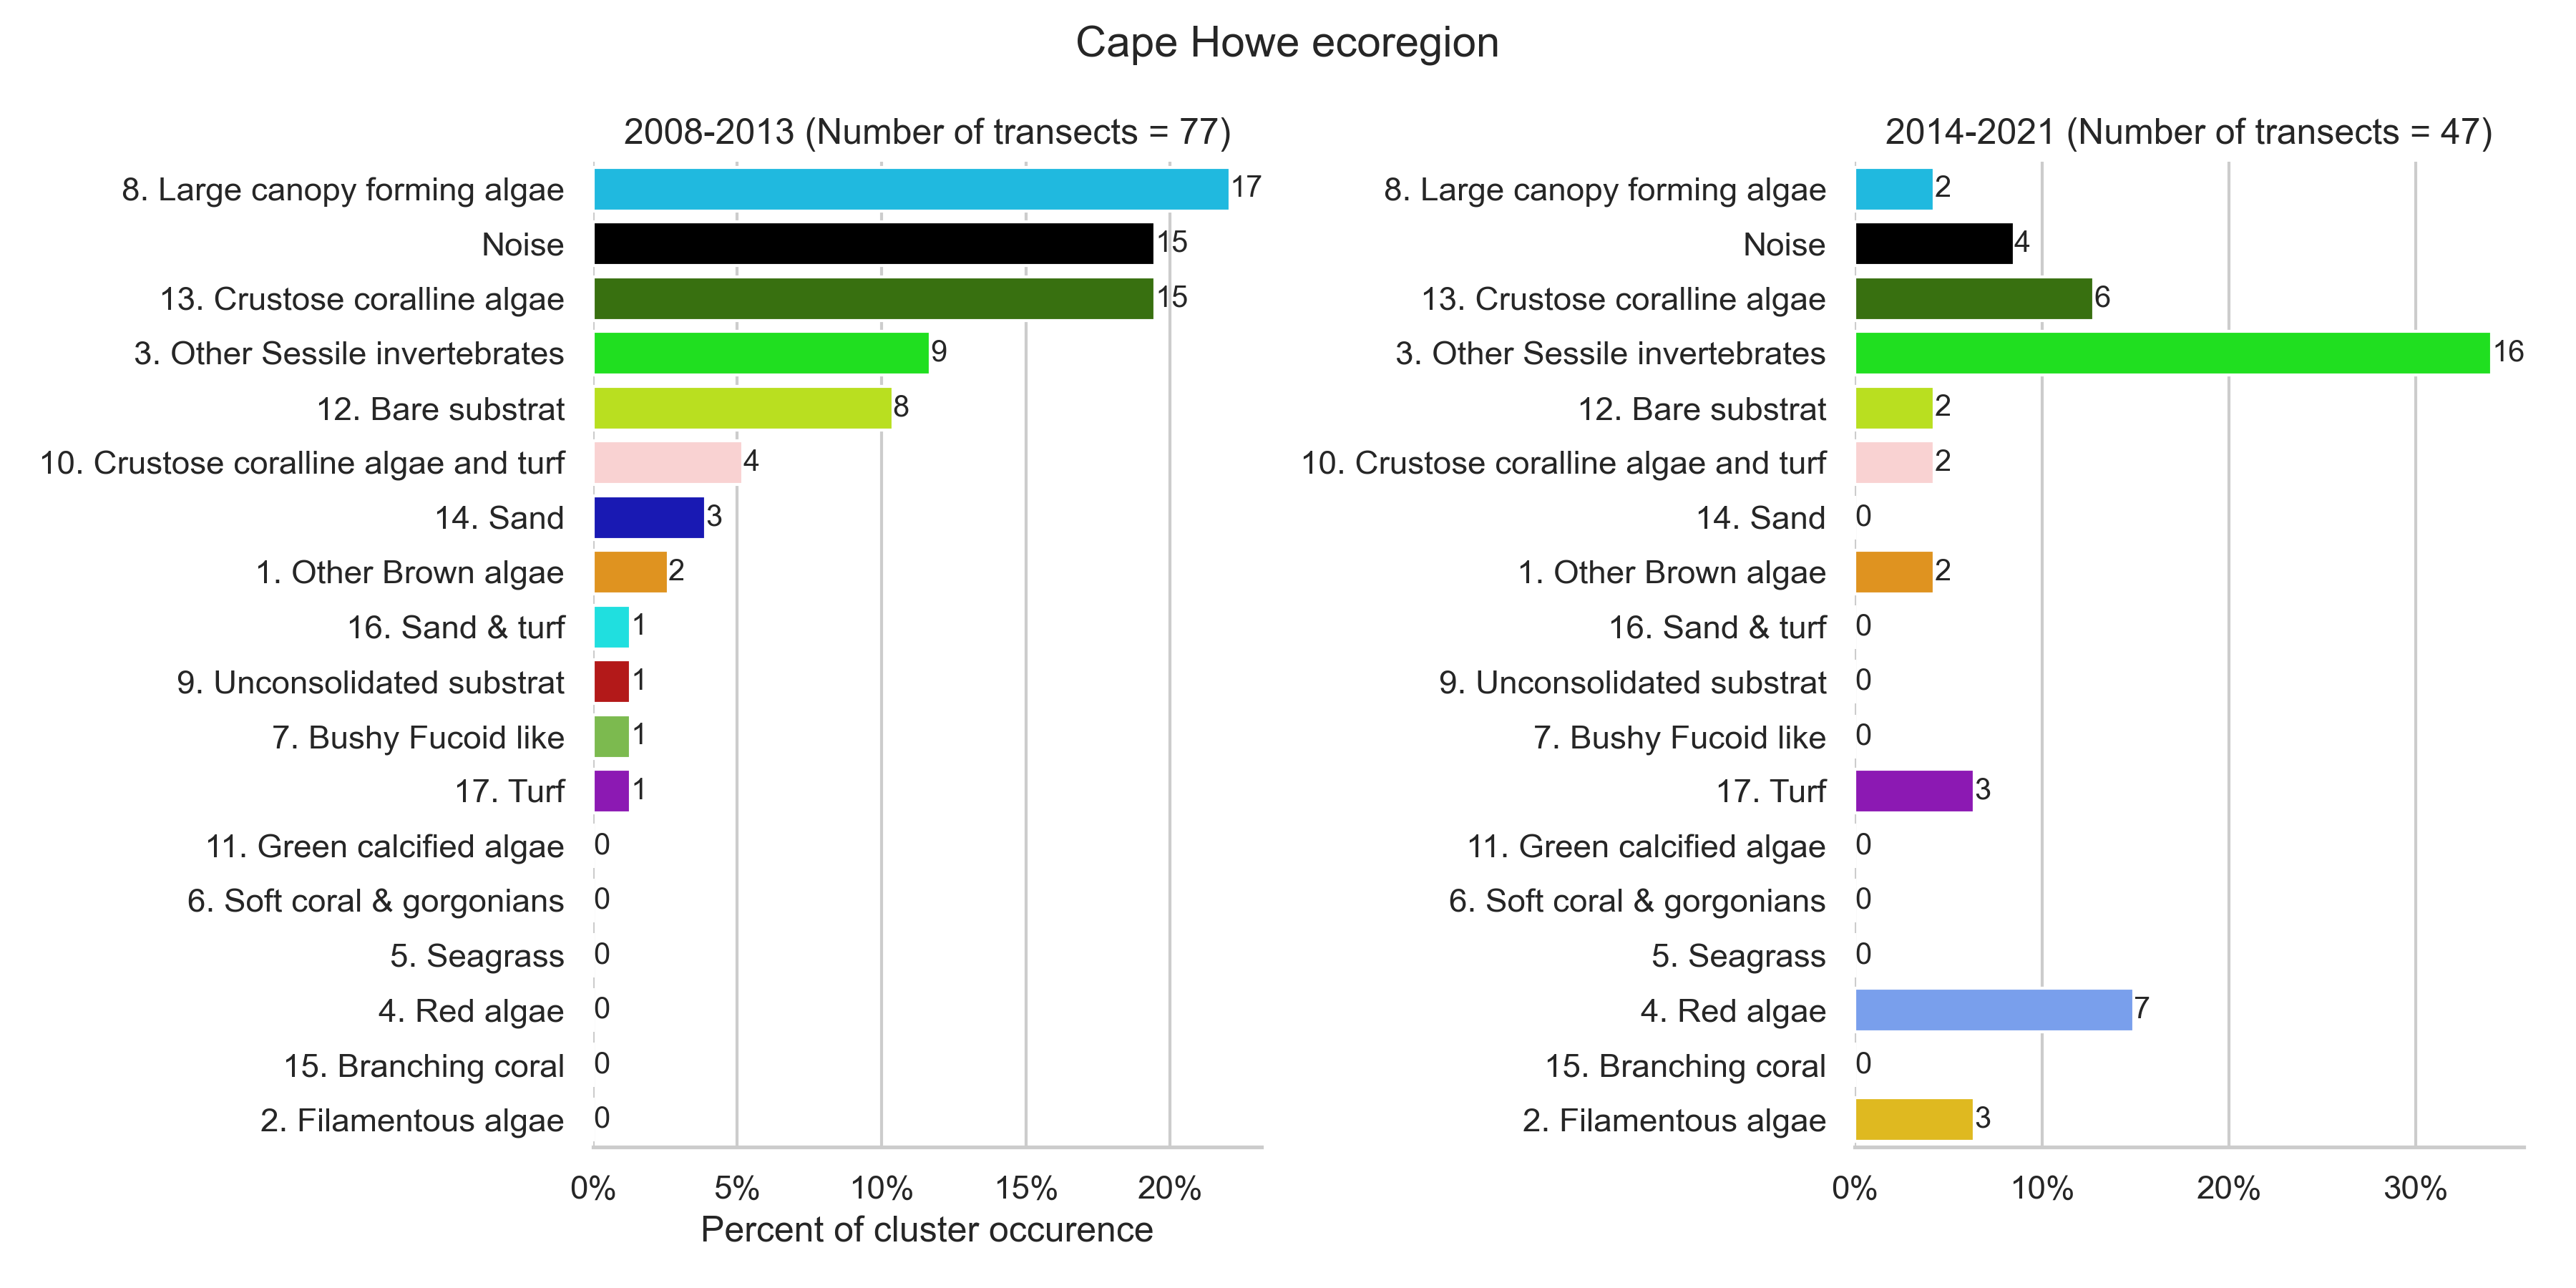
\includegraphics{03-Chapitre2/figures/supplementary/08-temporal_change_ecoregion_CapeHowe.png}
\caption{Bar graph of the proportion of different clusters for the
period 2008-2013 and 2015-2021 for sites that were sampled at least once
in each of the two periods for the Cape Howe
ecoregion.}\label{fig:chap2figS40}
}
\end{figure}

\begin{figure}
\hypertarget{fig:chap2figS39}{%
\centering
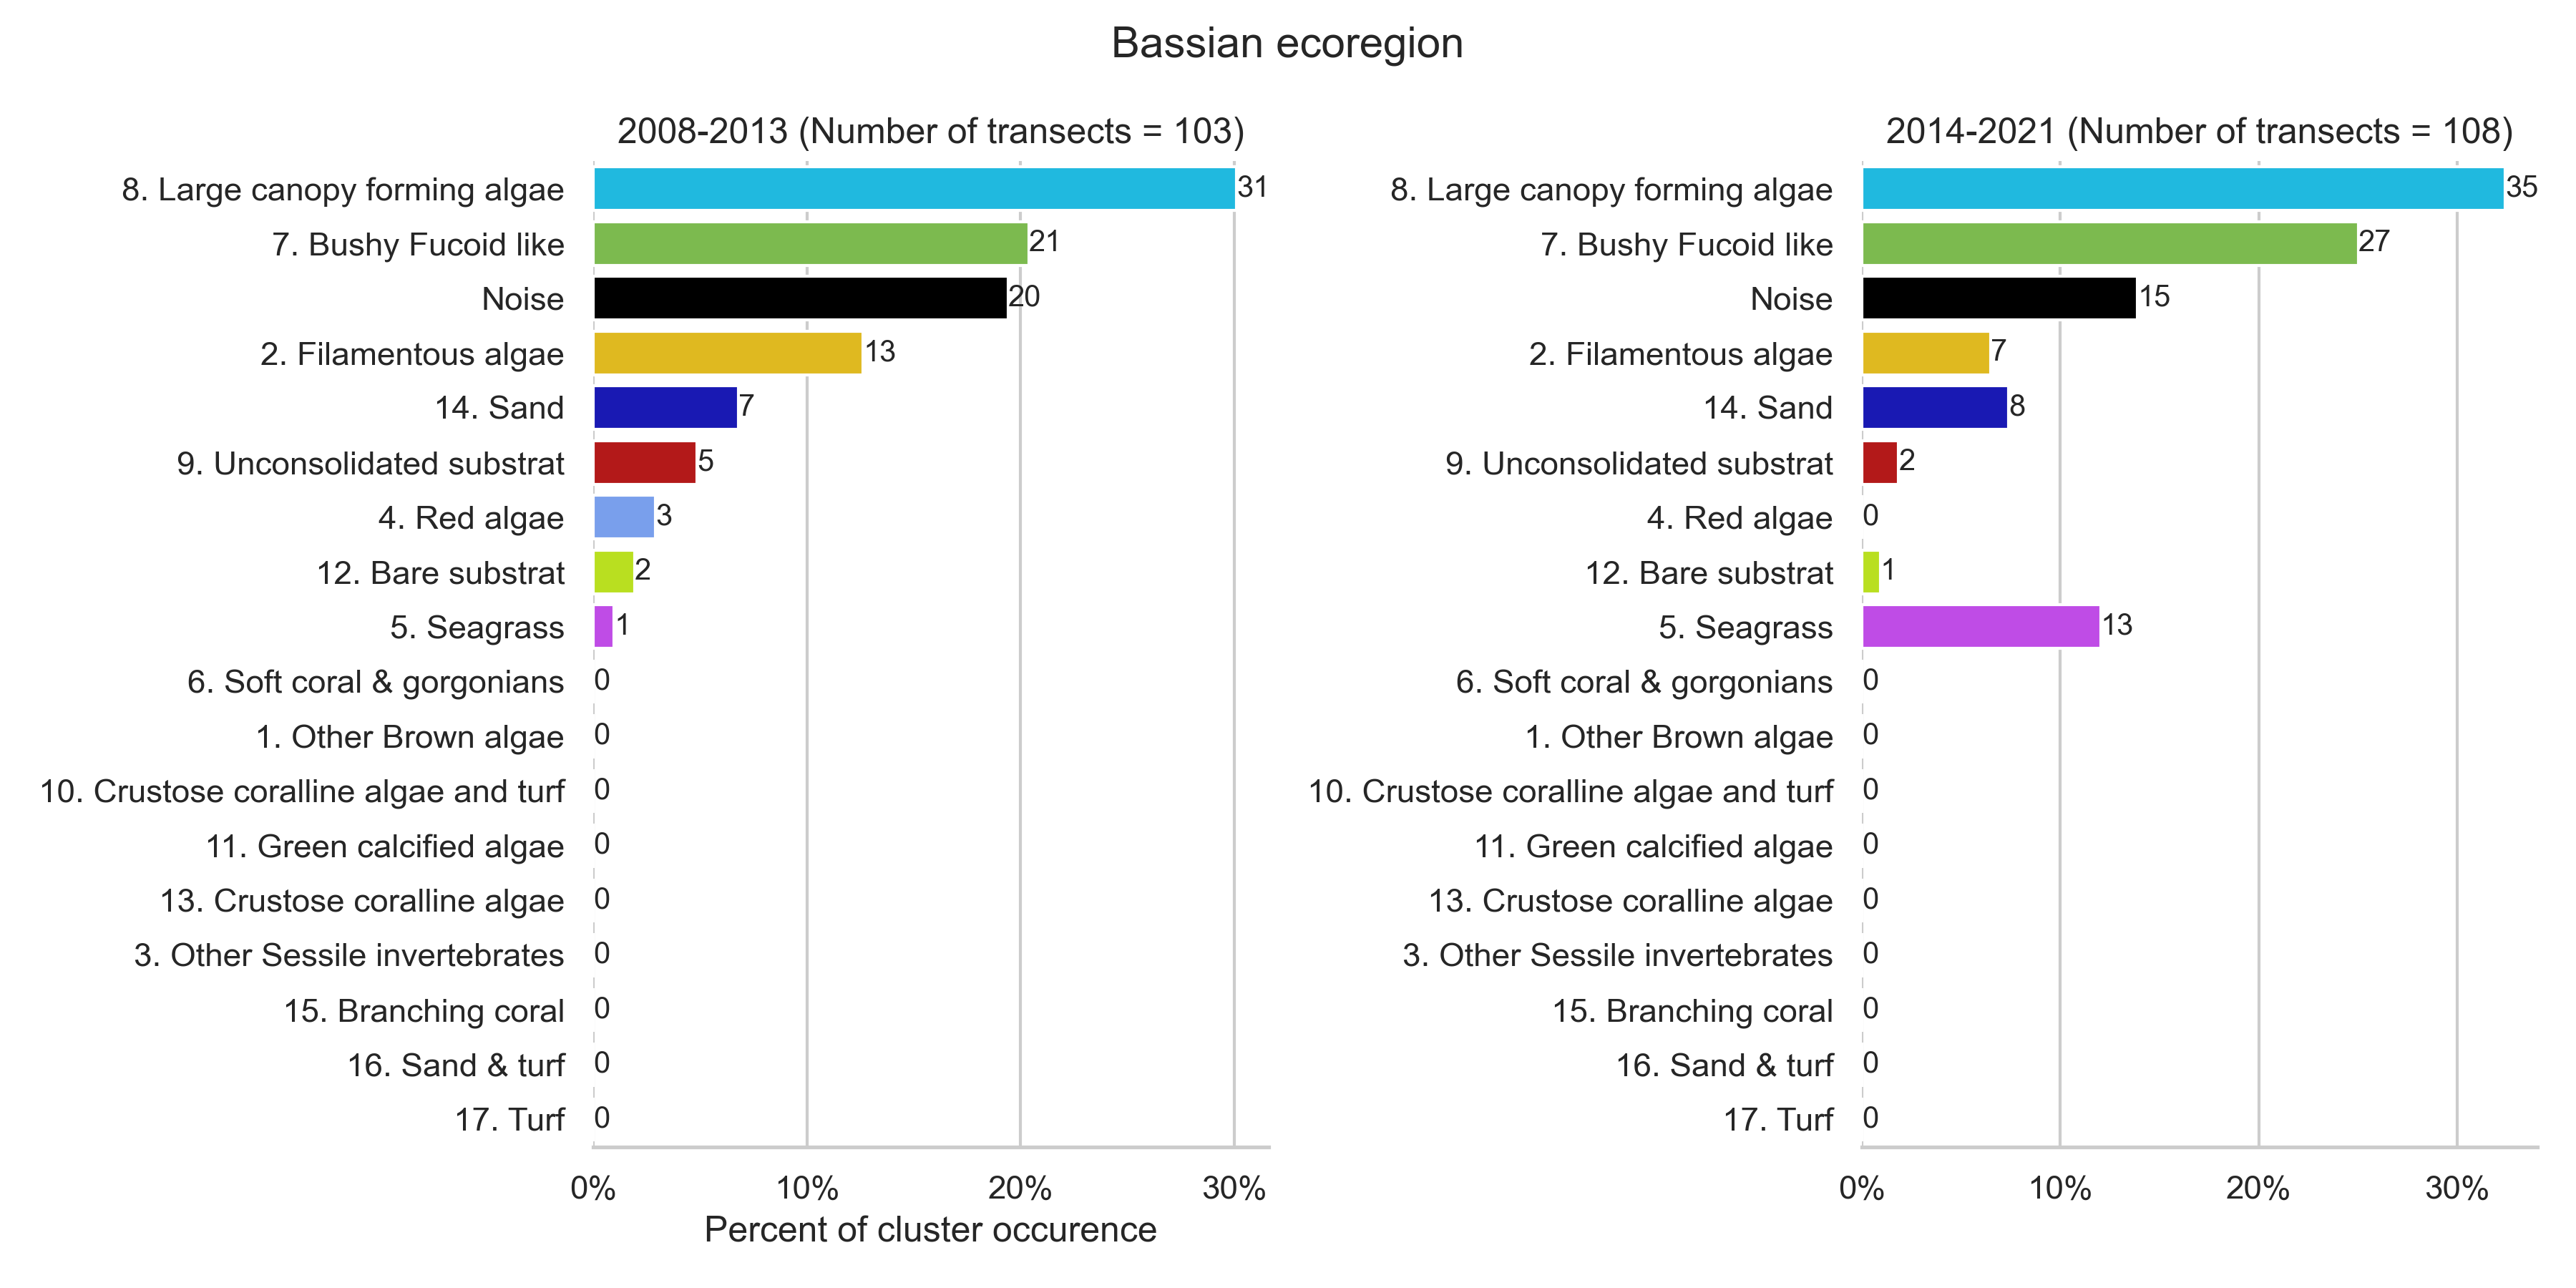
\includegraphics{03-Chapitre2/figures/supplementary/08-temporal_change_ecoregion_Bassian.png}
\caption{Bar graph of the proportion of different clusters for the
period 2008-2013 and 2015-2021 for sites that were sampled at least once
in each of the two periods for the Bassian
ecoregion.}\label{fig:chap2figS39}
}
\end{figure}

\begin{figure}
\hypertarget{fig:chap2figS41}{%
\centering
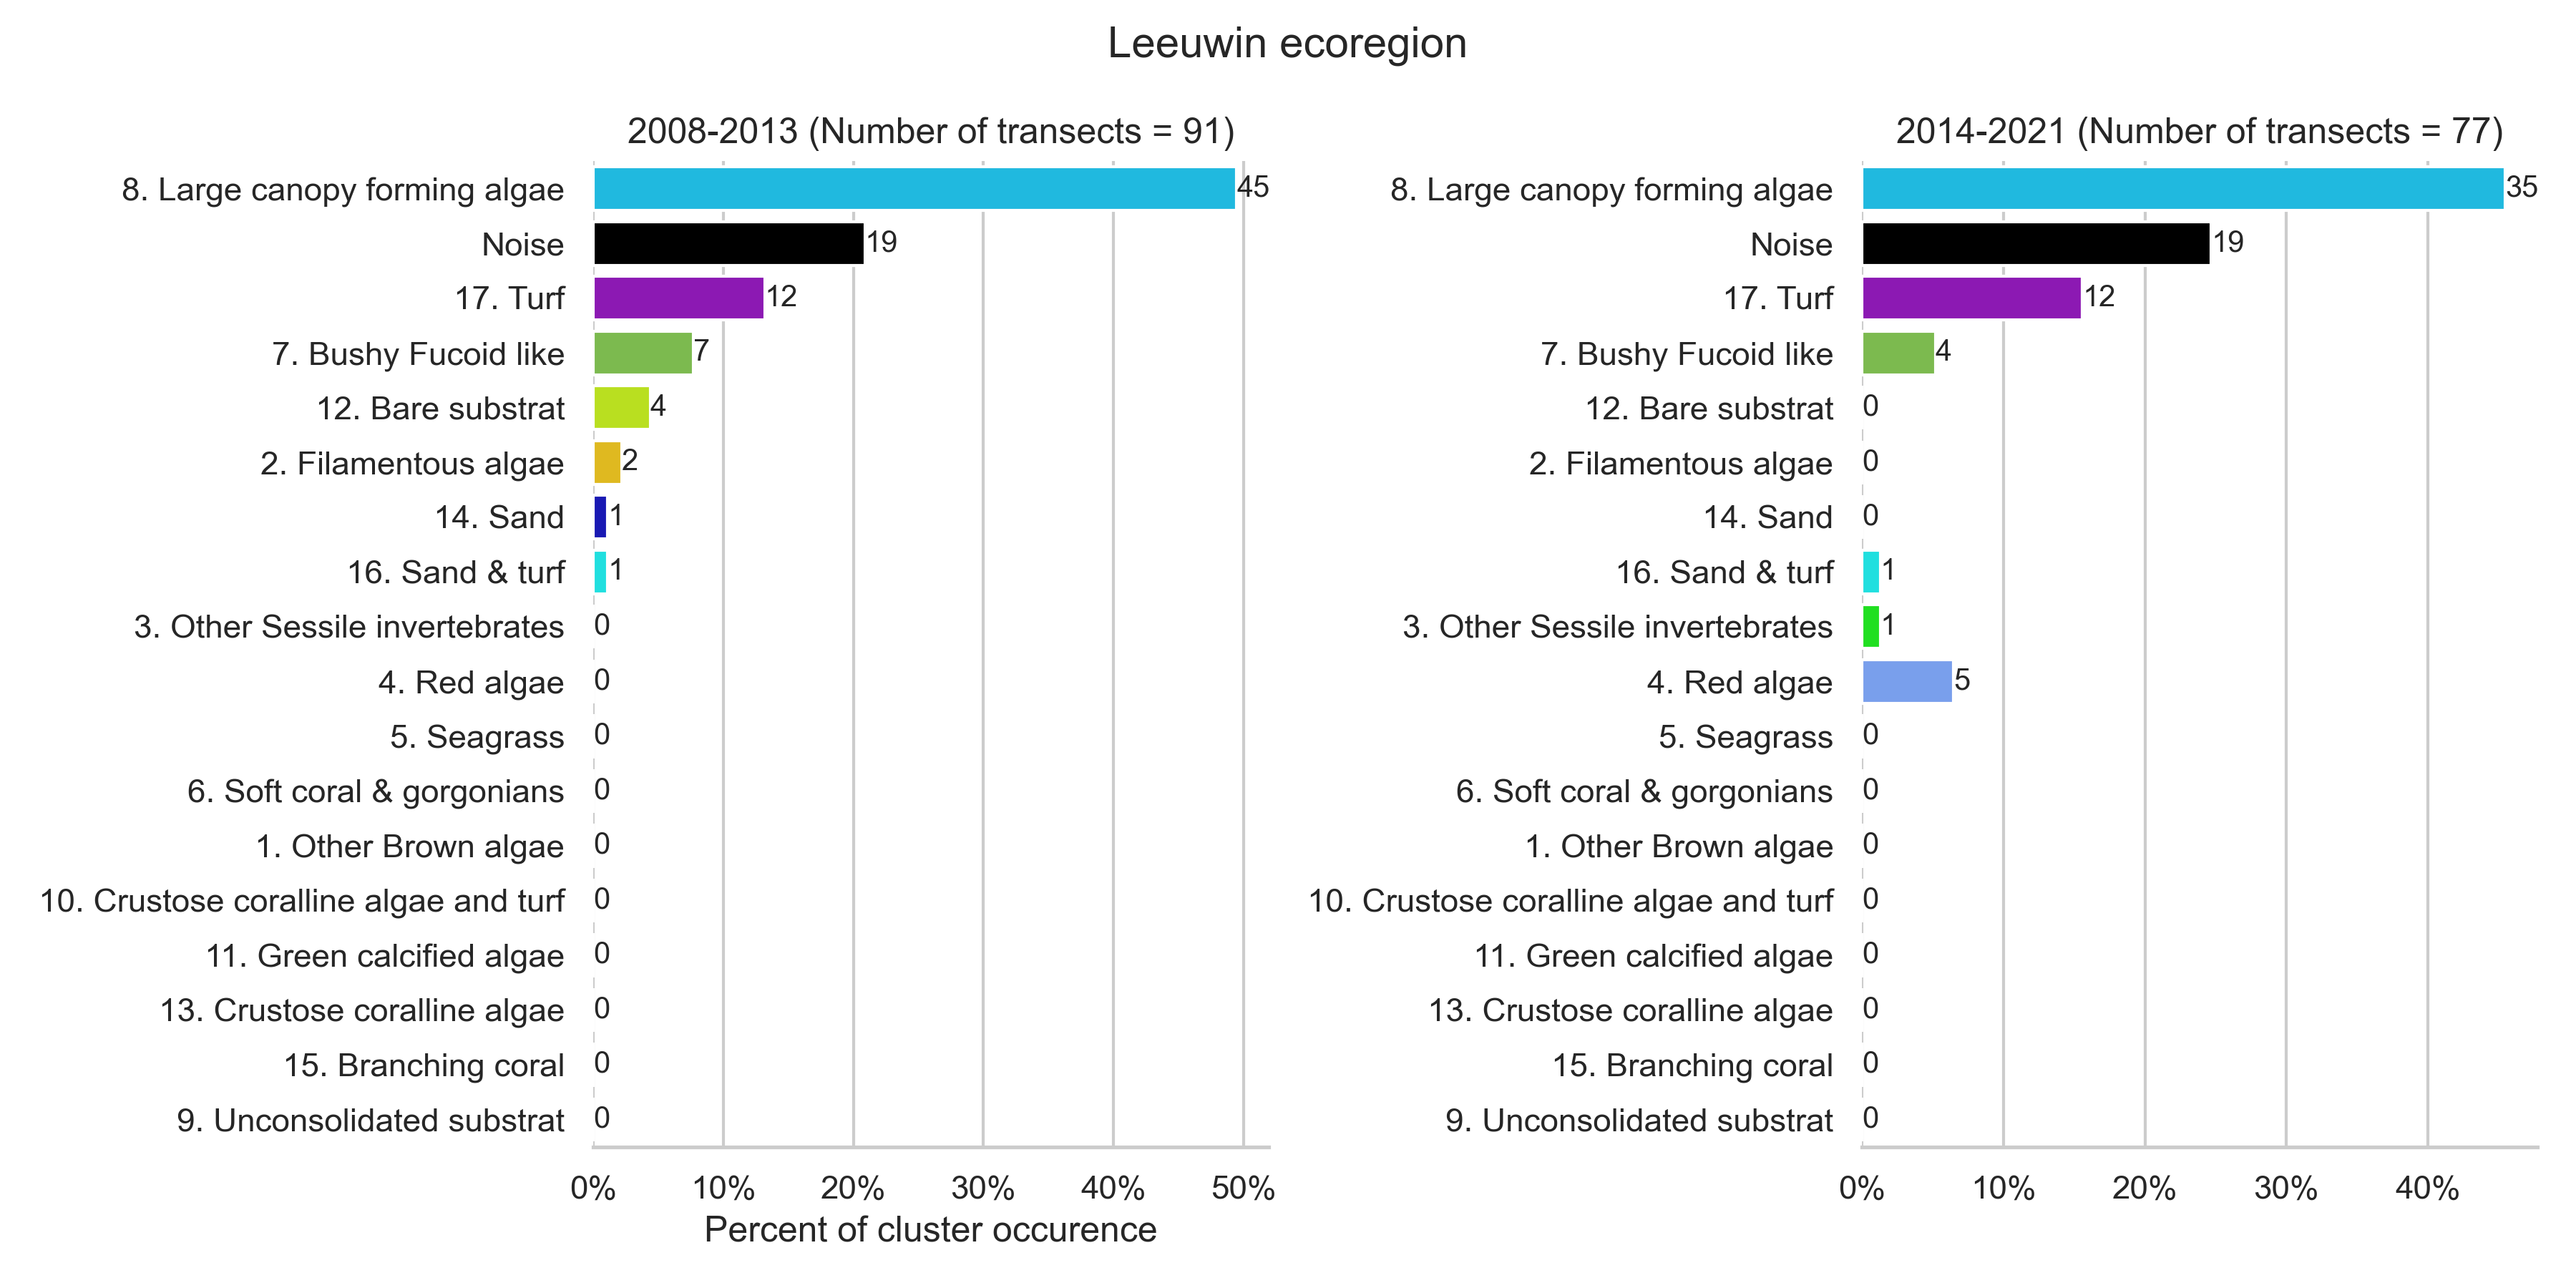
\includegraphics{03-Chapitre2/figures/supplementary/08-temporal_change_ecoregion_Leeuwin.png}
\caption{Bar graph of the proportion of different clusters for the
period 2008-2013 and 2015-2021 for sites that were sampled at least once
in each of the two periods for the Leeuwing
ecoregion.}\label{fig:chap2figS41}
}
\end{figure}

\begin{figure}
\hypertarget{fig:chap2figS43}{%
\centering
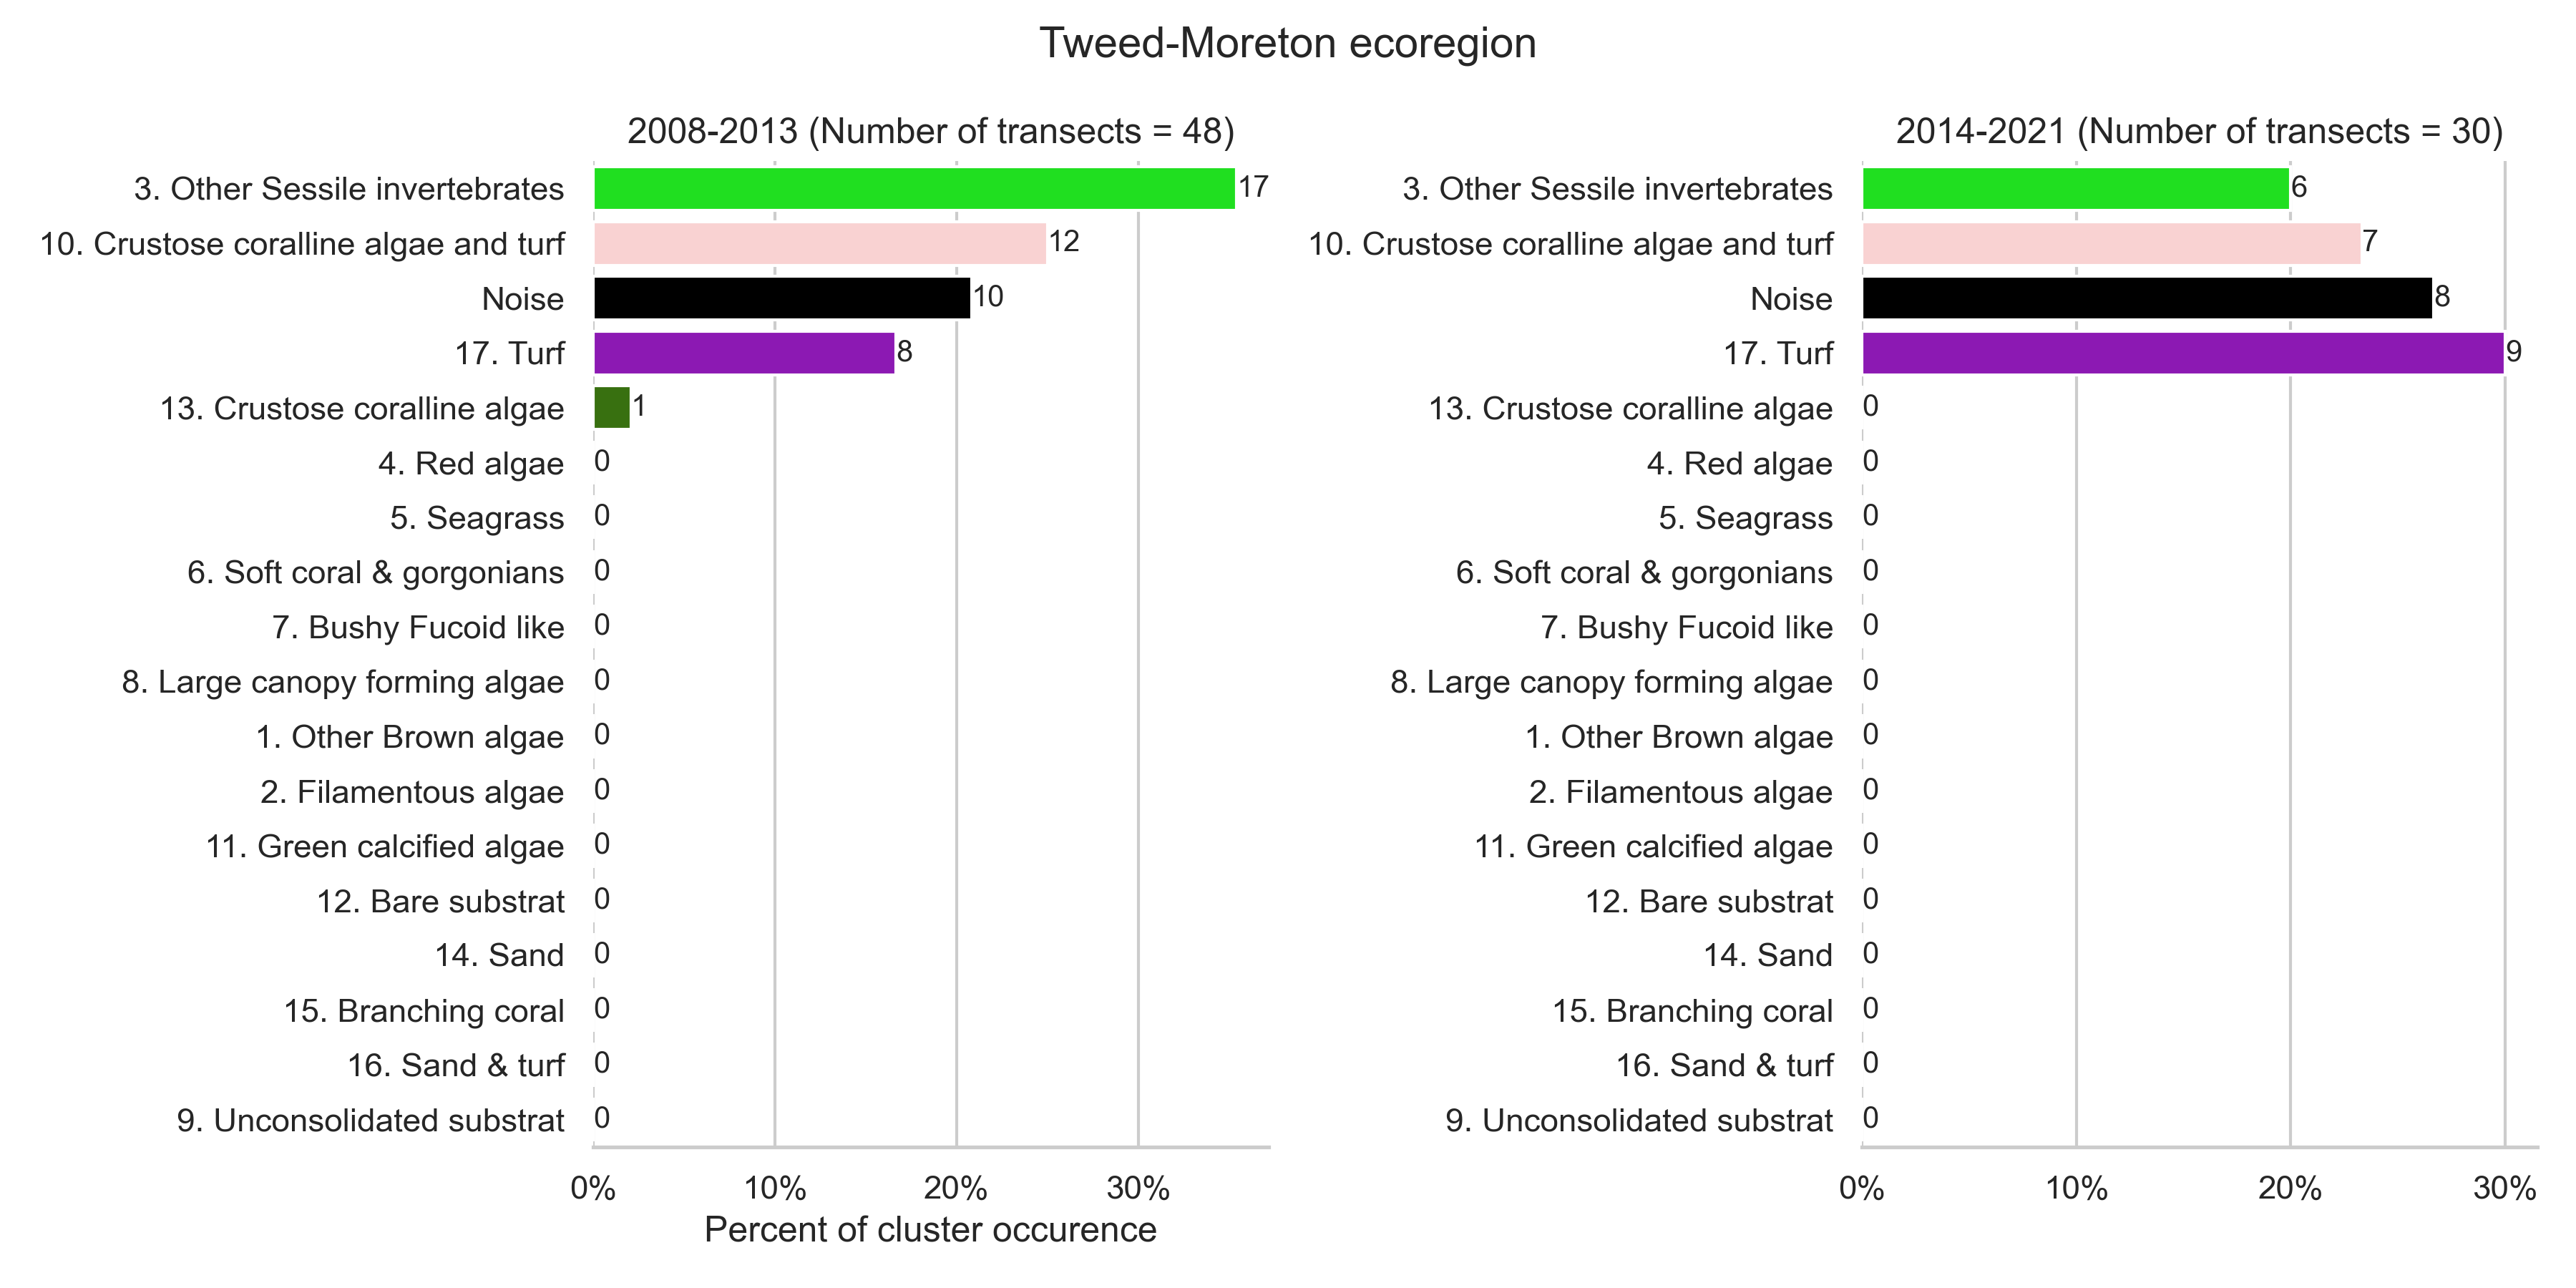
\includegraphics{03-Chapitre2/figures/supplementary/08-temporal_change_ecoregion_Tweed-Moreton.png}
\caption{Bar graph of the proportion of different clusters for the
period 2008-2013 and 2015-2021 for sites that were sampled at least once
in each of the two periods for the Tweed-Moreton
ecoregion.}\label{fig:chap2figS43}
}
\end{figure}

% Restore all parameters as default

\let\sectionmark\oldsectionmark

\captionsetup[figure]{list=yes}
\captionsetup[table]{list=yes}

\renewcommand{\thefigure}{\arabic{figure}}
\renewcommand{\thetable}{\arabic{table}}   

\counterwithin{figure}{chapter}
\counterwithin{table}{chapter}

% End of subappendices environment
\AtEndEnvironment{subappendices}{%
}